% Documento principal da monografia de Thales Gomes Batista
\NeedsTeXFormat{LaTeX2e}
\documentclass[a4paper,12pt]{monografia}

\usepackage[portuguese, colorinlistoftodos, textsize=tiny]{todonotes}
\usepackage{amsmath,amsthm,amsfonts,amssymb}
\usepackage[mathcal]{eucal}
\usepackage{latexsym}
\usepackage[portuguese]{babel}
\usepackage[utf8]{inputenc}
\usepackage[T1]{fontenc}
\usepackage{setspace}
\usepackage{bm}
\usepackage[portuguese,algoruled,longend,linesnumbered]{algorithm2e}
\usepackage{listings}
\usepackage{graphicx}
\usepackage{hyperref}
\usepackage{booktabs}

\graphicspath{{Graphics/}}
\hypersetup{
  colorlinks,
  linkcolor=black,
  citecolor=black,
  urlcolor=black,
  bookmarksopen=true
}
\usepackage[alf,bibjustif]{abntex2cite}

\include{hifenizacao}

\begin{document}
% Informações pré-textuais adaptadas ao modelo UFJF
\titulo{Avaliação de uma Proposta de Adaptação do Algoritmo TCP CUBIC Utilizando Informações de RTT}
\autor{Thales Gomes Batista}
\nome{Thales}
\ultimonome{Batista}

\bacharelado
\curso{Ciência da Computação}
\dia{XX}
\mes{XX}
\ano{2026}
\cidade{Juiz de Fora}

\instituicao{Universidade Federal de Juiz de Fora}
\sigla{UFJF}
\unidadeacademica{Instituto de Ciências Exatas}
\departamento{Departamento de Ciência da Computação}

\orientador{Edelberto Franco Silva}
\ttorientador{Prof. Dr.}

% Dados de banca ainda não informados; manter campos do modelo sem preencher.
% \examinadorum{Nome do examinador}
% \ttexaminadorum{Titulação}
% \examinadordois{Nome do examinador}
% \ttexaminadordois{Titulação}

\maketitle


% Agradecimentos (texto do TCC original)
\agradecimento{Agradecimentos}
\end{center}

\vspace{1cm}
Agradeço primeiramente à minha família pelo apoio incondicional ao longo de toda a minha trajetória acadêmica e pessoal.

Agradeço ao meu orientador, Prof. Dr. Edelberto Franco Silva, pela paciência, disponibilidade e orientação técnica fundamentais para a condução desta pesquisa.

Agradeço aos colegas de curso e à Universidade Federal de Juiz de Fora (UFJF) pelo suporte estrutural e acadêmico durante a graduação.

% Resumo em português (mantido do TCC original)
\resumo{Resumo}
\end{center}
O controle de congestionamento é fundamental para a eficiência e a estabilidade das redes de computadores, pois regula a quantidade de dados em trânsito e a utilização dos enlaces compartilhados. Este trabalho investiga o comportamento dos algoritmos TCP CUBIC e TCP BBR e, a partir dessa comparação, apresenta uma variante do CUBIC denominada TCP CUBIC-RTT. A proposta incorpora informações relacionadas ao tempo de ida e volta (RTT) à estrutura original do CUBIC, utilizando o menor RTT observado em relação a um valor de referência para adaptar o fator de crescimento cúbico $C$ e o fator de redução multiplicativa $\beta$. Os coeficientes $\alpha$ e $\gamma$ controlam a intensidade dessas adaptações. A implementação foi realizada no simulador ns-3 e avaliada em três campanhas: uma comparação inicial entre CUBIC, BBR e CUBIC-RTT; uma campanha de robustez, com diferentes condições de rede e combinações de parâmetros; e uma campanha de coexistência, na qual quatro fluxos de cada variante compartilham o mesmo gargalo. Foram analisadas vazão, perda de pacotes, atraso médio, jitter e justiça entre fluxos. Na comparação inicial, o CUBIC-RTT manteve vazão agregada próxima à do CUBIC e apresentou jitter ligeiramente menor, mas também atraso médio superior e perda maior em parte dos cenários. Na campanha de coexistência, a vantagem de vazão do CUBIC-RTT aumentou com o atraso do gargalo, indicando que a adaptação pode alterar a distribuição de recursos entre algoritmos concorrentes. Os resultados mostram que a informação de RTT pode modificar o comportamento do CUBIC, mas seus efeitos dependem do cenário e envolvem compromissos entre as métricas avaliadas.

\noindent \textbf{Palavras-chave:} redes de computadores; controle de congestionamento; TCP CUBIC; TCP BBR; RTT; coexistência de fluxos; ns-3.

% Abstract (mantido do TCC original)
\resumo{Abstract}
\end{center}
Congestion control is essential to the efficiency and stability of computer networks because it regulates the amount of data in flight and the use of shared links. This work investigates TCP CUBIC and TCP BBR and, based on this comparison, presents a CUBIC variant named TCP CUBIC-RTT. The proposal incorporates round-trip time (RTT) information into the original CUBIC structure, using the minimum observed RTT relative to a reference value to adapt the cubic growth factor $C$ and the multiplicative reduction factor $\beta$. The coefficients $\alpha$ and $\gamma$ control the intensity of these adaptations. The implementation was developed in the ns-3 simulator and evaluated through three campaigns: an initial comparison among CUBIC, BBR, and CUBIC-RTT; a robustness campaign with different network conditions and parameter combinations; and a coexistence campaign in which four flows of each variant share the same bottleneck. Throughput, packet loss, average delay, jitter, and inter-flow fairness were analysed. In the initial comparison, CUBIC-RTT maintained aggregate throughput close to CUBIC and presented slightly lower jitter, but also higher average delay and higher packet loss in some scenarios. In the coexistence campaign, the throughput advantage of CUBIC-RTT increased with bottleneck delay, indicating that the adaptation can change resource allocation between competing algorithms. The results show that RTT information can modify CUBIC's behaviour, but its effects depend on the scenario and involve trade-offs among the evaluated metrics.

\noindent \textbf{Keywords:} computer networks; congestion control; TCP CUBIC; TCP BBR; RTT; flow coexistence; ns-3.

\tableofcontents
\thispagestyle{empty}
\listoffigures
\thispagestyle{empty}
\listoftables
\thispagestyle{empty}

% Abreviações
\chapter*{Lista de Abreviações}
\addcontentsline{toc}{chapter}{Lista de Abreviações}
\begin{tabular}{l l}
TCP & Transmission Control Protocol \\
RTT & Round-Trip Time \\
ns-3 & Network Simulator 3 \\
UFJF & Universidade Federal de Juiz de Fora \\
\end{tabular}

\pagestyle{ruledheader}

% Corpo do trabalho
\chapter{INTRODUÇÃO}
O crescimento contínuo do tráfego de dados e a diversificação das aplicações em tempo real colocam exigências cada vez maiores sobre a infraestrutura das redes de computadores. Nesse cenário, o protocolo de controle de transmissão (\textbf{TCP} --- \textit{Transmission Control Protocol})~\cite{rfc9293} assegura a entrega confiável e ordenada dos dados, mas seu desempenho em enlaces de alta capacidade e com vários fluxos concorrentes depende do \textbf{controle de congestionamento}~\cite{rfc5681}.

Ao longo das décadas, vários algoritmos foram propostos para repartir a largura de banda disponível sem saturar as filas dos roteadores. O \textbf{TCP CUBIC}~\cite{ha2008,rfc9438} tornou-se o algoritmo padrão em sistemas Linux. Em vez de crescer a janela de congestionamento de forma linear, como fazem os algoritmos clássicos da família Reno, o CUBIC usa uma função cúbica do tempo, o que o torna mais escalável em redes de alta velocidade (\textit{high-speed networks}).

O CUBIC, porém, é essencialmente orientado a perdas (\textit{loss-based}): ele só reduz a janela depois que uma perda acontece e, até lá, tende a manter a fila do gargalo cada vez mais cheia. O resultado é o aumento do atraso (\textit{bufferbloat}) e, em alguns casos, prejuízo à justiça (\textit{fairness}) entre fluxos concorrentes. A intensidade desse efeito varia com a topologia, o tamanho dos buffers e o tráfego concorrente, como mostram as comparações experimentais entre CUBIC e BBR~\cite{casas2022,ware2019}.

O \textbf{TCP BBR} (\textit{Bottleneck Bandwidth and Round-trip propagation time}), desenvolvido pelo Google, parte de outra ideia. Em vez de tratar a perda como o principal sinal de congestionamento, ele estima a largura de banda do gargalo e o menor tempo de ida e volta do caminho, e ajusta o envio a partir desse modelo~\cite{cardwell2017}.

Foi dessa diferença de abordagem que nasceu este trabalho, que desenvolve e avalia, no simulador \textbf{ns-3}, uma variante do CUBIC chamada \textbf{TCP CUBIC-RTT}. A proposta usa informações de RTT para ajustar dois parâmetros do algoritmo: o coeficiente $\alpha$, que regula o quanto o crescimento da janela se adapta, e o coeficiente $\gamma$, que regula a redução da janela depois de um congestionamento.

\section{JUSTIFICATIVA}
A proposta surgiu da comparação entre a forma como CUBIC e BBR controlam o envio de dados. O CUBIC guia o crescimento da janela por uma função cúbica e reage ao congestionamento principalmente por meio de perdas; o BBR, por sua vez, trabalha com estimativas da largura de banda do gargalo e do RTT de propagação. Dessa diferença veio a pergunta que orienta todo o trabalho: acrescentar uma informação de RTT à lógica do CUBIC muda seu comportamento de forma relevante?

Vale deixar claro que não se parte da premissa de que a adaptação seja melhor do que os algoritmos existentes. Trata-se de uma hipótese a ser testada. Por isso, a proposta mantém a estrutura geral do CUBIC e altera apenas o cálculo de dois fatores, um ligado ao crescimento e outro à redução da janela, usando uma medida de RTT como referência.

A investigação começa com a comparação entre CUBIC, BBR e CUBIC-RTT sob diferentes atrasos no enlace de gargalo. Em seguida, os experimentos são ampliados para variar a largura de banda, a quantidade de fluxos, o atraso dos enlaces de acesso e os coeficientes de adaptação. Avaliar a proposta em condições variadas, e não em um único cenário, acompanha a orientação do RFC 9743~\cite{rfc9743} para a análise de novos algoritmos de controle de congestionamento. São analisadas vazão, perda de pacotes, atraso médio, jitter e justiça entre fluxos.

\section{OBJETIVOS}
O objetivo geral é comparar os algoritmos TCP CUBIC e TCP BBR e desenvolver e avaliar uma variante do CUBIC, o TCP CUBIC-RTT, que incorpora uma medida de RTT à adaptação de fatores do controle de congestionamento.

Os objetivos específicos são:
\begin{itemize}
    \item \textbf{Fundamentar} os conceitos de controle de congestionamento em redes TCP, com ênfase no CUBIC, no BBR e nas métricas de avaliação;
    \item \textbf{Comparar inicialmente} CUBIC e BBR em cenários controlados, identificando diferenças de comportamento que motivem a proposta;
    \item \textbf{Implementar} a variante TCP CUBIC-RTT no código-fonte do \texttt{ns-3}, preservando a estrutura geral do CUBIC e introduzindo adaptação baseada em RTT;
    \item \textbf{Executar campanhas experimentais} com diferentes atrasos de gargalo, larguras de banda, quantidades de fluxos, atrasos de acesso e combinações dos coeficientes de adaptação;
    \item \textbf{Coletar e analisar} vazão, perda de pacotes, atraso médio, jitter e justiça entre fluxos, além dos rastros das variáveis internas do TCP;
    \item \textbf{Avaliar criticamente} em quais condições a proposta altera o comportamento do CUBIC e quais compromissos aparecem em relação ao algoritmo original e ao BBR;
    \item \textbf{Investigar a coexistência} entre fluxos CUBIC e CUBIC-RTT que compartilham o mesmo gargalo, verificando se a adaptação favorece ou prejudica uma das variantes.
\end{itemize}

\section{ORGANIZAÇÃO DO TRABALHO}
O Capítulo 2 apresenta a fundamentação teórica: o controle de congestionamento no TCP, o CUBIC, o BBR, a simulação por eventos discretos e as métricas de avaliação. O Capítulo 3 descreve a metodologia, com a topologia, as três campanhas experimentais, a matriz de parâmetros e os cuidados estatísticos. O Capítulo 4 detalha a implementação do TCP CUBIC-RTT e as decisões de instrumentação. O Capítulo 5 apresenta e discute os resultados da comparação inicial, da campanha de robustez e do experimento de coexistência. O Capítulo 6 reúne as considerações finais, as contribuições e os trabalhos futuros.

\chapter{FUNDAMENTAÇÃO TEÓRICA}
O controle de congestionamento é um dos mecanismos mais importantes para a estabilidade da Internet, pois evita o colapso por saturação de roteadores e enlaces. Este capítulo reúne os conceitos necessários para acompanhar o restante do trabalho.

\section{Controle de Congestionamento no TCP}
O TCP opera na camada de transporte e oferece um canal confiável e orientado a conexões sobre redes IP que, em geral, só fazem entrega pelo melhor esforço (\textit{best-effort})~\cite{rfc9293,kurose2017}. Para que os emissores não sobrecarreguem roteadores cujos buffers são finitos, o TCP mantém uma janela de congestionamento (\textit{congestion window}, $cwnd$) que limita a quantidade de dados em trânsito (\textit{bytes in flight}) antes da chegada das confirmações (\textit{ACKs}). O limiar de partida lenta (\textit{slow start threshold}, $ssthresh$) define quando a janela deixa de crescer de forma exponencial e passa a crescer de forma mais cautelosa~\cite{rfc5681}.

Algoritmos clássicos como o TCP Reno seguem o esquema AIMD (\textit{Additive Increase, Multiplicative Decrease}): a janela cresce linearmente a cada RTT e é reduzida pela metade diante de uma perda~\cite{rfc5681,kurose2017}. Esse esquema é robusto, mas se mostra ineficiente em redes de alta velocidade e alto produto largura de banda-atraso (\textit{Bandwidth-Delay Product}, BDP), porque a janela leva muito tempo para se recuperar depois de uma perda.

\section{O Algoritmo TCP CUBIC}
O TCP CUBIC foi proposto para corrigir essa limitação em redes de alta velocidade~\cite{ha2008}. Em vez de crescer linearmente, a janela é função cúbica do tempo $t$ decorrido desde a última redução~\cite{rfc9438}:
\begin{equation}
    W_{cubic}(t) = C\,(t-K)^3 + W_{max}, \qquad K = \sqrt[3]{\frac{W_{max}\,(1-\beta)}{C}}
\end{equation}
onde $W_{max}$ é a janela registrada imediatamente antes da última redução, $C$ é o fator de escala do crescimento cúbico, $\beta$ é a fração da janela preservada após uma perda e $K$ é o tempo que a função leva para voltar a $W_{max}$. A especificação atual adota $C=0{,}4$ e $\beta=0{,}7$~\cite{rfc9438}.

O formato da curva explica o comportamento do algoritmo. Logo após uma redução, a janela cresce depressa; ao se aproximar de $W_{max}$, o crescimento desacelera, o que dá estabilidade a esse ponto; ultrapassado $W_{max}$, a curva volta a acelerar para sondar se há capacidade adicional. Como o crescimento depende do tempo e não do RTT, o CUBIC é adequado a caminhos de longa distância.

Por reagir sobretudo a perdas, o CUBIC pode deixar a fila do gargalo crescer antes de perceber o congestionamento, o que eleva a latência e favorece o \textit{bufferbloat}. O tamanho desse efeito depende da topologia, dos buffers, da capacidade dos enlaces e da concorrência entre fluxos.

\section{O Algoritmo TCP BBR}
O TCP BBR~\cite{cardwell2017} segue uma abordagem baseada em modelo. Ele estima continuamente a largura de banda máxima do gargalo ($BtlBw$, \textit{bottleneck bandwidth}) e o tempo mínimo de propagação do RTT ($RTprop$). Com essas estimativas, calcula o BDP e regula a taxa de envio e a quantidade de dados em trânsito para usar a capacidade do gargalo sem manter filas longas.

Esse mecanismo não garante ausência de filas ou perdas. O desempenho e a justiça do BBR variam com a versão do algoritmo, o tamanho dos buffers, a topologia e a presença de outros fluxos, inclusive fluxos CUBIC~\cite{ware2019,casas2022}.

\section{Simulação de Redes por Eventos Discretos no ns-3}
Experimentos em redes físicas costumam ser difíceis de reproduzir e de isolar variável por variável. Por isso, recorre-se a simuladores de eventos discretos, entre os quais o \textbf{ns-3}~\cite{ns3}. O \texttt{ns-3} é um simulador de código aberto escrito em C++ (com \textit{bindings} para Python) que modela a pilha de protocolos IP, canais, enlaces e algoritmos de controle de tráfego. Sua arquitetura modular permite implementar novas variantes de transporte e executar cenários controlados e repetíveis, requisito importante para a pesquisa acadêmica.

\section{Métricas de Avaliação de Desempenho}
O comportamento dos protocolos de transporte é analisado com um conjunto de métricas de qualidade de serviço:
\begin{itemize}
    \item \textbf{Vazão (\textit{throughput}):} taxa de dados úteis entregues ao destino por unidade de tempo, em Mbps.
    \item \textbf{Atraso médio unidirecional:} intervalo entre o envio de um pacote e sua recepção no destino, conforme o FlowMonitor. Não deve ser confundido com o RTT, que é o tempo de ida e volta observado pela conexão.
    \item \textbf{Taxa de perda de pacotes:} percentual de pacotes descartados no caminho por congestionamento e estouro de filas.
    \item \textbf{Jitter:} média das variações absolutas entre os atrasos de pacotes consecutivos, conforme os registros do FlowMonitor. A noção de variação de atraso de pacotes é a mesma formalizada na métrica IPDV do IETF~\cite{rfc3393}; aqui, porém, vale a definição operacional do FlowMonitor.
    \item \textbf{Índice de Justiça de Jain:} medida adimensional da equidade na divisão de recursos entre $n$ fluxos~\cite{jain1984}, dada por
    \begin{equation}
        J = \frac{\left( \sum_{i=1}^{n} x_i \right)^2}{n \sum_{i=1}^{n} x_i^2}
    \end{equation}
    em que $x_i$ é a vazão média do $i$-ésimo fluxo. O índice varia em $[1/n, 1]$, e valores próximos de $1$ indicam distribuição mais equilibrada.
\end{itemize}

\chapter{METODOLOGIA}

A metodologia combina o desenvolvimento da variante TCP CUBIC-RTT com sua avaliação experimental. A abordagem é empírico-quantitativa: simulações no ns-3 comparam o comportamento da proposta com o do CUBIC e do BBR. O processo teve as seguintes etapas: implementação da proposta, definição das topologias e dos parâmetros, execução das campanhas, coleta das métricas e processamento dos dados.

\section{Ambiente de Simulação}

Os experimentos foram realizados no simulador ns-3~\cite{ns3}, que permite controlar as características dos enlaces, os atrasos de propagação, a largura de banda e a quantidade de fluxos concorrentes. Com isso, os algoritmos são comparados em condições experimentais equivalentes.

Os cenários foram implementados em C++ sobre os módulos de rede e transporte do ns-3. Para registrar o comportamento dos fluxos, usaram-se mecanismos de rastreamento de eventos e o módulo FlowMonitor.

\section{Arquitetura da Topologia Experimental}

A topologia tem dois roteadores intermediários, Gateway A e Gateway B, ligados por um enlace compartilhado que é o gargalo da rede. Os nós de origem abrem fluxos TCP que atravessam o Gateway A, passam pelo gargalo e chegam aos nós de destino pelo Gateway B. Dessa forma, vários fluxos disputam a capacidade de um mesmo enlace, o que permite observar como cada algoritmo se comporta sob competição por recursos.

A largura de banda e o atraso de propagação do gargalo são configuráveis. Os enlaces de acesso dos nós finais têm parâmetros próprios, mantidos fixos em cada cenário, de modo que a variação analisada venha principalmente do gargalo e da quantidade de fluxos.

\section{Parâmetros e Variáveis Experimentais}

Os experimentos foram organizados em três campanhas complementares. A primeira compara TCP CUBIC, TCP BBR e TCP CUBIC-RTT em uma topologia controlada. A segunda amplia a avaliação, variando os parâmetros da proposta e as condições de rede. A terceira investiga a coexistência entre fluxos CUBIC e CUBIC-RTT no mesmo gargalo. A ampliação dos cenários segue a orientação de avaliar novos algoritmos sob condições diversas de rede~\cite{rfc9743}.

\subsection{Campanha Comparativa Inicial}

Os parâmetros comuns da campanha inicial são:

\begin{itemize}
    \item Largura de banda do gargalo: 2 Mbps;
    \item Largura de banda dos enlaces de acesso: 10 Mbps;
    \item Atraso dos enlaces de acesso: 45 ms;
    \item Número de fluxos concorrentes: 4;
    \item Duração de cada simulação: 100 segundos;
    \item Número de repetições: 5;
    \item Atrasos do gargalo: 10 ms, 50 ms e 100 ms.
\end{itemize}

Com três algoritmos, três atrasos e cinco repetições, a campanha compreende 45 execuções.

\subsection{Campanha de Robustez e Variação de Parâmetros}
\label{sec:robustez}

A segunda campanha investiga o comportamento dos algoritmos sob outras condições de rede e com diferentes configurações do CUBIC-RTT. Foram definidos três cenários:

\begin{itemize}
    \item \textbf{bw1\_f4:} gargalo de 1 Mbps, quatro fluxos e atraso de acesso de 45 ms;
    \item \textbf{bw2\_f8:} gargalo de 2 Mbps, oito fluxos e atraso de acesso de 45 ms;
    \item \textbf{access100:} gargalo de 2 Mbps, quatro fluxos e atraso de acesso de 100 ms.
\end{itemize}

Em todos os cenários, os enlaces de acesso têm 10 Mbps. Os atrasos do gargalo voltam a ser 10 ms, 50 ms e 100 ms, com cinco repetições por configuração.

A campanha contempla quinze configurações de algoritmo e parâmetros: o CUBIC original, o BBR, o CUBIC-RTT na configuração de referência ($\alpha=0{,}25$ e $\gamma=0{,}05$) e doze configurações adicionais do CUBIC-RTT, obtidas pela variação de $\alpha$ e $\gamma$:

\begin{itemize}
    \item $\alpha=0{,}10$: $\gamma \in \{0{,}00; 0{,}025; 0{,}05; 0{,}10\}$;
    \item $\alpha=0{,}25$: $\gamma \in \{0{,}00; 0{,}025\}$;
    \item $\alpha=0{,}50$: $\gamma \in \{0{,}00; 0{,}025\}$;
    \item $\alpha=0{,}75$: $\gamma \in \{0{,}00; 0{,}025; 0{,}05; 0{,}10\}$.
\end{itemize}

O total de execuções da campanha é

\begin{equation}
N = 3 \times 15 \times 3 \times 5 = 675.
\end{equation}

Separar as campanhas permite avaliar primeiro os algoritmos tradicionais e a proposta e, depois, a influência dos parâmetros internos do CUBIC-RTT em cenários mais diversos.

\subsection{Campanha de Coexistência entre CUBIC e CUBIC-RTT}

A terceira campanha foi concebida para observar diretamente a interação entre as duas variantes quando disputam a mesma capacidade de transmissão. Foram executados oito fluxos TCP simultâneos: os fluxos 0, 2, 4 e 6 utilizaram CUBIC, enquanto os fluxos 1, 3, 5 e 7 utilizaram CUBIC-RTT, com $\alpha=0{,}25$ e $\gamma=0{,}05$. A alternância foi mantida também na atribuição dos enlaces de acesso, de modo que cada algoritmo tivesse um fluxo em cada uma das quatro condições de atraso de acesso.

O gargalo compartilhado foi configurado com largura de banda de 10 Mbps e atrasos de 10 ms, 50 ms e 100 ms. Os enlaces de acesso operaram a 1 Gbps e foram configurados com atrasos de 10 ms, 30 ms, 60 ms e 90 ms, cada condição atribuída a um par de fluxos, um de cada algoritmo. O experimento utilizou aquecimento de 20 segundos, seguido por 300 segundos de medição, cinco repetições por atraso e início dos fluxos com deslocamento aleatório de até dois segundos. A configuração de fila utilizou um tamanho equivalente a um BDP.

Assim, a campanha compreendeu:
\begin{equation}
N_{\text{coexistência}} = 3 \times 5 = 15
\end{equation}
execuções, totalizando 120 registros de fluxos de dados no FlowMonitor. A vazão foi comparada pela média dos quatro fluxos de cada algoritmo em cada repetição. A perda foi consolidada a partir dos pacotes transmitidos e perdidos, enquanto atraso e jitter foram calculados a partir dos valores dos quatro fluxos de cada grupo.

A atribuição dos algoritmos foi conferida pelos endereços de origem: os endereços \texttt{10.0.1.1}, \texttt{10.0.3.1}, \texttt{10.0.5.1} e \texttt{10.0.7.1} identificam os fluxos CUBIC; os endereços \texttt{10.0.2.1}, \texttt{10.0.4.1}, \texttt{10.0.6.1} e \texttt{10.0.8.1} identificam os fluxos CUBIC-RTT. Essa separação permite observar se a vantagem de uma variante ocorre sem confundir os resultados com a diferença de atraso dos enlaces de acesso.

\subsection{Execução e consolidação das campanhas}

As três campanhas totalizam 735 simulações: 45 na comparação inicial, 675 na campanha de robustez e 15 na campanha de coexistência. Nas duas primeiras campanhas, cada simulação contém quatro fluxos nos cenários \texttt{bw1\_f4} e \texttt{access100}, e oito fluxos no cenário \texttt{bw2\_f8}. A campanha de coexistência utiliza oito fluxos em todas as execuções.

Como o FlowMonitor registra fluxos nos dois sentidos da comunicação, os registros foram processados para separar os fluxos de dados das conexões reversas utilizadas para os reconhecimentos (ACKs). Essa filtragem evita contabilizar o tráfego de retorno como se fosse tráfego útil independente. Nas duas primeiras campanhas, foram consolidados 3.780 registros de fluxos de dados. A campanha de coexistência acrescentou 120 registros, correspondentes a oito fluxos em cada uma das quinze execuções.

Os rastros internos também foram auditados. Os 3.780 arquivos de CWND e os 3.780 de SSThresh (7.560 no total) estavam completos, sem pares ausentes, erros ou avisos. Nos dados do FlowMonitor, os totais de bytes e pacotes transmitidos e recebidos foram confirmados, e a taxa de perda e o atraso médio foram reproduzidos exatamente a partir dos valores brutos. O recálculo do jitter apresentou erro médio de cerca de $5{,}57\times10^{-6}$ ms (máximo de $2{,}03\times10^{-4}$ ms), e o índice de Jain, diferença média de aproximadamente 0,00028 (máxima de 0,00349), atribuídas à precisão numérica e à forma de agregação por fluxo. Por serem muito pequenas, essas diferenças não alteram a interpretação dos resultados.

A aleatoriedade das simulações foi controlada pelas sementes do ns-3: todas as execuções usam $Seed = 1$, e o identificador de repetição \texttt{RngRun} assume valores de 1 a 5. Assim, as condições de cada repetição podem ser reproduzidas, desde que se mantenham as versões do código, os parâmetros e a configuração dos geradores.

Há, porém, uma ressalva importante. Identificadores diferentes não garantem independência estatística, pois alguns algoritmos se comportam de forma determinística em condições idênticas. Foi o que se observou na campanha inicial: CUBIC e CUBIC-RTT produziram valores idênticos entre repetições em algumas métricas, enquanto o BBR variou. Por isso, médias e desvios são tratados como estatísticas descritivas das execuções, e não como base para afirmar significância estatística onde não há variabilidade efetiva.

\section{Coleta das Métricas de Desempenho}

Os dados foram coletados por dois mecanismos complementares: o FlowMonitor e o rastreamento de variáveis internas do TCP.

\subsection{Métricas obtidas pelo FlowMonitor}

O FlowMonitor forneceu, para cada fluxo:

\begin{itemize}
    \item \textbf{Vazão:} dados recebidos com sucesso por unidade de tempo, em Mbps;
    \item \textbf{Perda de pacotes:} relação entre os pacotes transmitidos e os que não chegaram ao destino;
    \item \textbf{Atraso médio:} média dos atrasos dos pacotes recebidos;
    \item \textbf{Jitter:} variação dos atrasos entre pacotes consecutivos.
\end{itemize}

As métricas foram analisadas por fluxo e de forma agregada por simulação, considerando os totais e os intervalos de tempo do conjunto de fluxos. O RTT, por sua vez, é analisado à parte, a partir do rastreamento da variável interna do TCP.

\subsection{Métricas internas do TCP}

Foram rastreadas quatro variáveis internas, o que permite observar a evolução do controle de congestionamento ao longo do tempo:

\begin{itemize}
    \item \textbf{CWND:} janela de congestionamento do emissor, em bytes;
    \item \textbf{SSThresh:} limiar de transição entre as fases de crescimento da janela;
    \item \textbf{RTT:} tempo de ida e volta observado pela conexão;
    \item \textbf{InFlight:} quantidade de dados enviados e ainda não reconhecidos.
\end{itemize}

\section{Processamento e Consolidação dos Dados}

Os arquivos gerados são organizados por algoritmo, cenário, atraso e repetição. Scripts em Python leem os arquivos, identificam os fluxos relevantes, calculam estatísticas e consolidam os resultados em arquivos CSV. O processamento associa as métricas de cada fluxo ao respectivo cenário e verifica a consistência dos dados: registros ausentes, duplicações e divergências entre totais agregados e valores individuais.

A justiça na distribuição da banda foi avaliada com o Índice de Jain~\cite{jain1984}, calculado a partir da vazão ou da quantidade de dados recebida pelos fluxos, conforme a análise.

\section{Tratamento Estatístico e Limitações das Repetições}

Os resultados são organizados por configuração e repetição. Quando há variabilidade entre as execuções, usam-se medidas descritivas (média, mínimo e máximo). Algumas configurações, no entanto, podem produzir execuções idênticas, sobretudo quando algoritmo e cenário não introduzem variação aleatória efetiva entre as repetições, e a interpretação dos resultados considera essa possibilidade.

\chapter{IMPLEMENTAÇÃO DO TCP CUBIC-RTT}

O TCP CUBIC-RTT foi implementado diretamente no código-fonte do ns-3, a partir do TCP CUBIC que o simulador já oferece. A implementação está nos arquivos \texttt{tcp-cubic-rtt.cc} e \texttt{tcp-cubic-rtt.h}.

A ideia central é incorporar informações de RTT ao crescimento e à redução da janela do CUBIC. Para isso, foram introduzidos dois coeficientes de sensibilidade, $\alpha$ e $\gamma$, que controlam a intensidade da adaptação do fator de crescimento cúbico $C$ e do fator de redução multiplicativa $\beta$ após o congestionamento.

\section{Estrutura Geral da Modificação}

O CUBIC original usa uma função cúbica para determinar o crescimento da janela, com parâmetros que definem a velocidade e a forma desse crescimento. No CUBIC-RTT, o fator de escala cúbico deixa de ser fixo e passa a ser ajustado conforme o RTT observado pela conexão. De forma análoga, o fator de redução multiplicativa usado após a detecção de perdas também passa a considerar a condição de atraso. A estrutura geral do CUBIC é mantida: a adaptação entra apenas nos pontos que calculam o crescimento e o limiar de congestionamento.

\section{Adaptação Baseada no RTT}

O mecanismo se apoia em duas grandezas: o menor RTT observado pela conexão, \texttt{m\_delayMin}, e um RTT de referência, \texttt{m\_rttReference}, fixado em 200 ms na configuração de referência dos experimentos. Note que a variável usada é o mínimo observado, e não a amostra instantânea de RTT. A referência serve de ponto de comparação: ela indica se o atraso mínimo da conexão está acima ou abaixo do nível considerado adequado.

A razão entre os dois valores é
\begin{equation}
rttRatio = \frac{m\_delayMin}{m\_rttReference}
\end{equation}
e sua diferença em relação à referência é normalizada e limitada ao intervalo $[-1, 1]$:
\begin{equation}
x = clamp(rttRatio - 1.0, -1.0, 1.0)
\end{equation}

Esse limite evita que RTTs extremos provoquem alterações desproporcionais nos parâmetros adaptativos. Se o menor RTT observado fica abaixo da referência, $x$ é negativo; se a ultrapassa, $x$ é positivo. Como a formulação parte do valor mínimo, ela mede a relação entre o atraso mínimo da conexão e a referência configurada e, por isso, não detecta aumentos transitórios de RTT causados pelo enfileiramento.

\section{Adaptação do Fator de Crescimento Cúbico}

O primeiro mecanismo atua sobre o fator $C$, que controla a agressividade do crescimento da janela. O fator adaptativo é
\begin{equation}
C_{adaptive} =
m\_c \times (1.0 + m\_alpha \times x)
\end{equation}
onde $m\_c$ é o fator cúbico original, $m\_alpha$ é o coeficiente $\alpha$ de sensibilidade ao RTT e $x$ é a variação normalizada do RTT em relação à referência. Quanto maior o valor de $\alpha$, maior a influência de $x$ sobre $C$; valores menores produzem uma adaptação mais moderada. Variar $\alpha$ permite, desse modo, investigar diferentes níveis de sensibilidade do crescimento da janela ao atraso da rede.

\section{Adaptação do Fator de Redução Multiplicativa}

O segundo mecanismo atua sobre o fator $\beta$, que define a proporção da janela mantida após um evento de perda:
\begin{equation}
\beta_{calc} =
m\_beta + m\_gamma \times x
\end{equation}
Para que o resultado respeite os limites da implementação, aplica-se uma função de limitação:
\begin{equation}
\beta_{adaptive} =
clamp(\beta_{calc}, m\_betaMin, m\_betaMax)
\end{equation}

O coeficiente $\gamma$ determina, assim, a influência de $x$ sobre o fator multiplicativo. Como $\beta$ é a fração da janela preservada, valores maiores correspondem a uma redução menos acentuada e valores menores, a uma redução mais forte.

As duas equações devem ser lidas em conjunto. Quando $x$ é positivo, tanto $C_{adaptive}$ quanto $\beta_{adaptive}$ tendem a aumentar: o crescimento cúbico fica mais intenso e uma fração maior da janela é preservada após a perda. Quando $x$ é negativo, ocorre o contrário. Não se pode afirmar, portanto, que todo aumento de RTT leva a uma redução mais conservadora da janela: o efeito depende do sinal de $x$ e do RTT de referência escolhido.

\section{Parâmetros Utilizados na Implementação}

Os parâmetros $\alpha$ e $\gamma$ são configuráveis a cada simulação. A configuração de referência da comparação experimental é:

\begin{itemize}
    \item Fator cúbico original: $C=0{,}4$~\cite{rfc9438};
    \item Fator de redução original: $\beta=0{,}7$~\cite{rfc9438};
    \item RTT de referência: 200 ms;
    \item $\alpha=0{,}25$;
    \item $\gamma=0{,}05$;
    \item Limite mínimo de $\beta$: 0,65;
    \item Limite máximo de $\beta$: 0,85.
\end{itemize}

Na campanha de robustez, $\alpha$ e $\gamma$ são variados para avaliar a influência de diferentes níveis de sensibilidade ao RTT.

\section{Organização do Código e Fluxo de Execução}

A implementação foi distribuída entre o modelo do protocolo e o programa responsável por montar e executar os cenários. Os arquivos da variante ficam no diretório \texttt{src/internet/model}. O arquivo \url{tcp-cubic-rtt.cc} contém a lógica executável do algoritmo, enquanto \url{tcp-cubic-rtt.h} declara a classe, seus atributos e as interfaces utilizadas pelo ns-3.

A adaptação do fator cúbico é concentrada no cálculo de $C$ adaptativo, implementado pela rotina \texttt{CalculateAdaptiveC()}. Esse valor é utilizado pelo mecanismo de crescimento da janela, integrado às rotinas \texttt{IncreaseWindow()} e \texttt{Update()}, que preservam a lógica temporal do CUBIC: início de uma época, cálculo do ponto de origem da curva, determinação de $K$ e atualização da janela em direção ao alvo cúbico. A adaptação não substitui a função cúbica por um modelo de taxa de envio diferente; ela altera o fator que controla sua escala.

A redução após congestionamento é tratada em \texttt{GetSsThresh()}. Nesse ponto, a implementação calcula o valor adaptativo de $\beta$, aplica os limites mínimo e máximo configurados e utiliza o resultado para determinar o novo limiar de congestionamento. A rotina \texttt{HystartUpdate()} permanece relacionada ao mecanismo de partida lenta, enquanto as informações de RTT são mantidas para alimentar o cálculo adaptativo. Com isso, as mudanças ficam concentradas nos pontos de crescimento e de reação à perda, sem eliminar os demais mecanismos do CUBIC.

Os principais atributos expostos pela implementação são o fator cúbico base, o RTT de referência, os coeficientes $\alpha$ e $\gamma$ e os limites de $\beta$. Na configuração de referência, foram utilizados $C=0{,}4$, $\beta=0{,}7$, RTT de referência de 200 ms, $\alpha=0{,}25$, $\gamma=0{,}05$, $\beta_{\min}=0{,}65$ e $\beta_{\max}=0{,}85$. Os coeficientes são configuráveis na execução, o que permite automatizar a matriz experimental sem editar o código entre combinações.

O programa de experimentos está em \texttt{examples/tcp/cubic-experiment.cc} e gera o executável \texttt{cubic-experiment}. Ele configura os nós, os enlaces de acesso e o gargalo, instala a pilha TCP, cria os emissores e receptores, define o algoritmo de transporte e os parâmetros da simulação e, ao final, executa o monitoramento e grava os resultados. Entre os parâmetros de execução estão o protocolo, o número de fluxos, a largura de banda e o atraso dos enlaces, a duração, a ativação do rastreamento e do FlowMonitor e o diretório de saída. Um exemplo de execução da campanha inicial é:

\begin{verbatim}
./ns3 run "cubic-experiment --transport_prot=TcpCubic \
  --num_flows=4 --bandwidth=2Mbps --delay=10ms \
  --access_bandwidth=10Mbps --access_delay=45ms \
  --duration=100 --tracing=true --flow_monitor=true \
  --results_dir=../../results/cubic/cenario01"
\end{verbatim}

\section{Instrumentação e Rastreamento das Variáveis}

O programa experimental conecta callbacks aos rastros disponibilizados pela pilha TCP do ns-3. Foram utilizados registros de \texttt{CongestionWindow}, \texttt{SlowStartThreshold}, RTT, RTO, \texttt{BytesInFlight} e variáveis de sequência utilizadas para diagnóstico, como \texttt{NextTx} e \texttt{RxBuffer/NextRxSequence}. Os dados são gravados em arquivos temporais por fluxo, permitindo relacionar o instante de cada alteração com o comportamento observado no FlowMonitor.

Os rastros de CWND e SSThresh foram produzidos para as 3.780 conexões de dados das duas primeiras campanhas. Também foram gerados rastros de RTT e de quantidade de dados em trânsito para examinar a evolução temporal das conexões. A instrumentação complementa as métricas agregadas: a vazão, a perda, o atraso e o jitter mostram o resultado de cada execução, enquanto os rastros permitem observar como a janela de congestionamento e o estado da conexão evoluem ao longo do tempo.

\section{Dificuldades de Implementação e Decisões Técnicas}

A primeira dificuldade foi a própria topologia. A configuração inicial tinha enlaces independentes entre os gateways e os destinos, o que não representava a disputa de vários emissores por um único recurso compartilhado. A solução foi reorganizar a arquitetura com dois roteadores intermediários, Gateway A e Gateway B, ligados por um enlace comum configurado como gargalo, de modo que a competição entre os fluxos passasse a ocorrer de fato no enlace de interesse.

Outro obstáculo surgiu na conexão dos \textit{callbacks} de rastreamento. O caminho \texttt{RxBuffer/NextRxSequence}, acessado por \texttt{SocketList/1}, não correspondia ao \textit{socket} usado pelo fluxo; a troca para \texttt{SocketList/0} resolveu a associação. O episódio serviu de lembrete de que é preciso validar o caminho de rastreamento de cada \textit{socket}, em vez de presumir que todos os nós e conexões usam o mesmo índice.

O processamento dos resultados trouxe mais dois cuidados. O primeiro foi separar os fluxos de dados dos fluxos reversos de ACK criados pelo FlowMonitor; sem isso, o tráfego de reconhecimento seria contado como uma segunda transmissão de dados e distorceria a vazão e as demais métricas. O segundo veio da observação de execuções idênticas em CUBIC e CUBIC-RTT: variar o \texttt{RngRun} não gera, necessariamente, variação em todos os algoritmos. Esse ponto foi tratado de forma explícita na análise estatística, para não considerar repetições determinísticas como amostras independentes.

\chapter{RESULTADOS E DISCUSSÃO}
\label{cap:resultados}

Este capítulo reúne os resultados das três campanhas experimentais. A primeira estabelece a comparação entre CUBIC, BBR e CUBIC-RTT em condições controladas. A segunda verifica como a proposta se comporta quando a capacidade do gargalo, o número de fluxos e os coeficientes de adaptação são modificados. A terceira coloca CUBIC e CUBIC-RTT em competição direta, permitindo observar se a adaptação altera a divisão da capacidade disponível entre fluxos de algoritmos diferentes.

As médias apresentadas são descritivas. Como algumas configurações produziram resultados idênticos entre repetições, não se atribui significância estatística às diferenças sem uma fonte efetiva de variabilidade. As barras de erro dos gráficos representam a dispersão observada entre as execuções consideradas.

\section{Comparação Inicial entre CUBIC, BBR e CUBIC-RTT}

A campanha inicial utilizou quatro fluxos TCP concorrentes, gargalo de 2 Mbps, enlaces de acesso de 10 Mbps com atraso de 45 ms e duração de 100 segundos por execução. Foram avaliados atrasos de gargalo de 10 ms, 50 ms e 100 ms, com cinco repetições por algoritmo e cenário, totalizando 45 simulações.

A Tabela~\ref{tab:resultados-iniciais} apresenta as médias das cinco execuções. A vazão corresponde à taxa agregada de dados úteis recebidos, e o atraso é o unidirecional, obtido pelo FlowMonitor.

\begin{table}[htbp]
\centering
\caption{Médias da campanha comparativa inicial}
\label{tab:resultados-iniciais}
\small
\begin{tabular}{c l r r r r}
\toprule
\textbf{Atraso} & \textbf{Algoritmo} & \textbf{Vazão (Mbps)} & \textbf{Perda (\%)} & \textbf{Atraso (ms)} & \textbf{Jitter (ms)} \\
\midrule
10 ms & CUBIC & 1,980 & 1,43 & 311,71 & 1,632 \\
10 ms & CUBIC-RTT & 1,980 & 1,42 & 319,91 & 1,610 \\
10 ms & BBR & 1,942 & 17,58 & 337,51 & 1,060 \\
\midrule
50 ms & CUBIC & 1,968 & 1,90 & 409,79 & 1,650 \\
50 ms & CUBIC-RTT & 1,966 & 2,00 & 419,28 & 1,595 \\
50 ms & BBR & 1,926 & 18,35 & 449,15 & 1,100 \\
\midrule
100 ms & CUBIC & 1,968 & 2,26 & 532,50 & 1,718 \\
100 ms & CUBIC-RTT & 1,968 & 2,46 & 545,39 & 1,659 \\
100 ms & BBR & 1,917 & 19,32 & 583,06 & 1,190 \\
\bottomrule
\end{tabular}
\end{table}

\subsection{Vazão e perda de pacotes}

CUBIC e CUBIC-RTT atingiram vazões agregadas praticamente iguais nos três atrasos. A diferença máxima foi de 0,002 Mbps no cenário de 50 ms. Isso indica que, nessa configuração, a introdução da adaptação baseada em RTT não comprometeu a utilização agregada do gargalo.

A perda de pacotes, por outro lado, não apresentou uma vantagem uniforme. Em 10 ms, CUBIC-RTT registrou 1,42\%, ligeiramente abaixo dos 1,43\% do CUBIC. Em 50 ms, a perda foi de 2,00\% para a proposta e 1,90\% para o algoritmo original. Em 100 ms, os valores foram 2,46\% e 2,26\%, respectivamente. A diferença é pequena em termos absolutos, mas mostra que a adaptação não reduziu as perdas em todas as condições.

O BBR apresentou perda consideravelmente maior nos três cenários, entre 17,58\% e 19,32\%. Esse comportamento deve ser interpretado no contexto da topologia, dos buffers e da configuração utilizada. Ele não permite concluir que o BBR apresente necessariamente esse nível de perda em outras versões ou ambientes.

\begin{figure}[htbp]
\centering
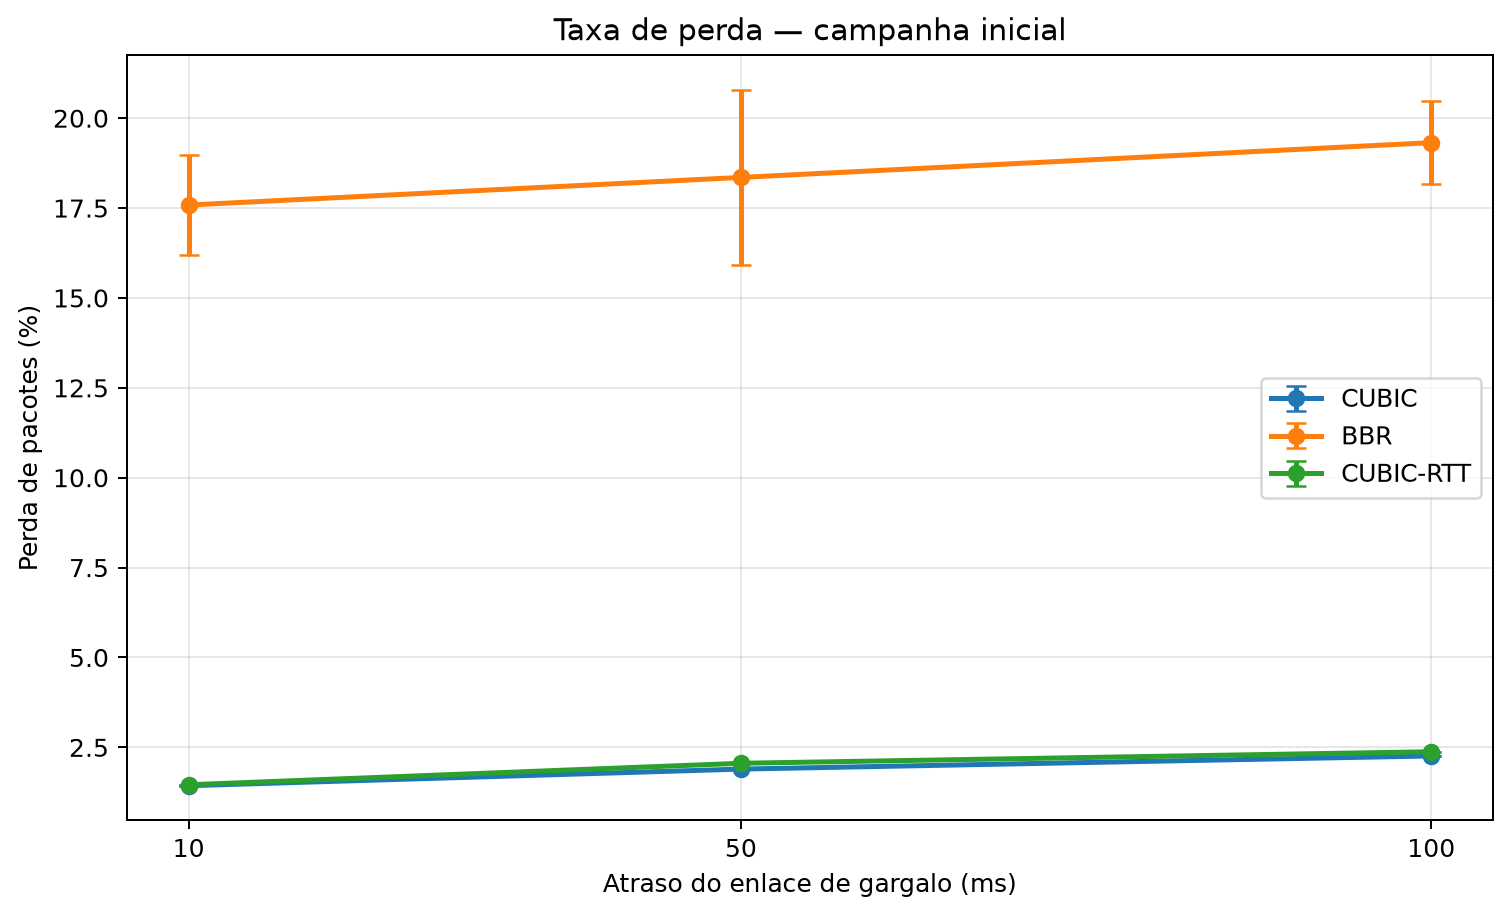
\includegraphics[width=0.88\textwidth]{inicial_packet_loss.png}
\caption{Taxa de perda de pacotes na campanha inicial.}
\label{fig:inicial-perda}
\end{figure}

\subsection{Atraso médio e RTT}

O atraso médio unidirecional aumentou à medida que o atraso configurado no gargalo passou de 10 ms para 100 ms. Para o CUBIC, as médias foram 311,71 ms, 409,79 ms e 532,50 ms. Para o CUBIC-RTT, foram 319,91 ms, 419,28 ms e 545,39 ms. Em todos os cenários, portanto, a proposta apresentou atraso médio superior, com diferenças de 8,20 ms, 9,49 ms e 12,89 ms.

Esse resultado é importante porque delimita o alcance da hipótese inicial. A utilização de RTT na adaptação não produziu, nessa campanha, uma redução do atraso médio de entrega. O mecanismo considera o menor RTT observado em relação a uma referência, e não atua diretamente sobre cada aumento instantâneo de atraso provocado pelo enfileiramento.

\begin{figure}[htbp]
\centering
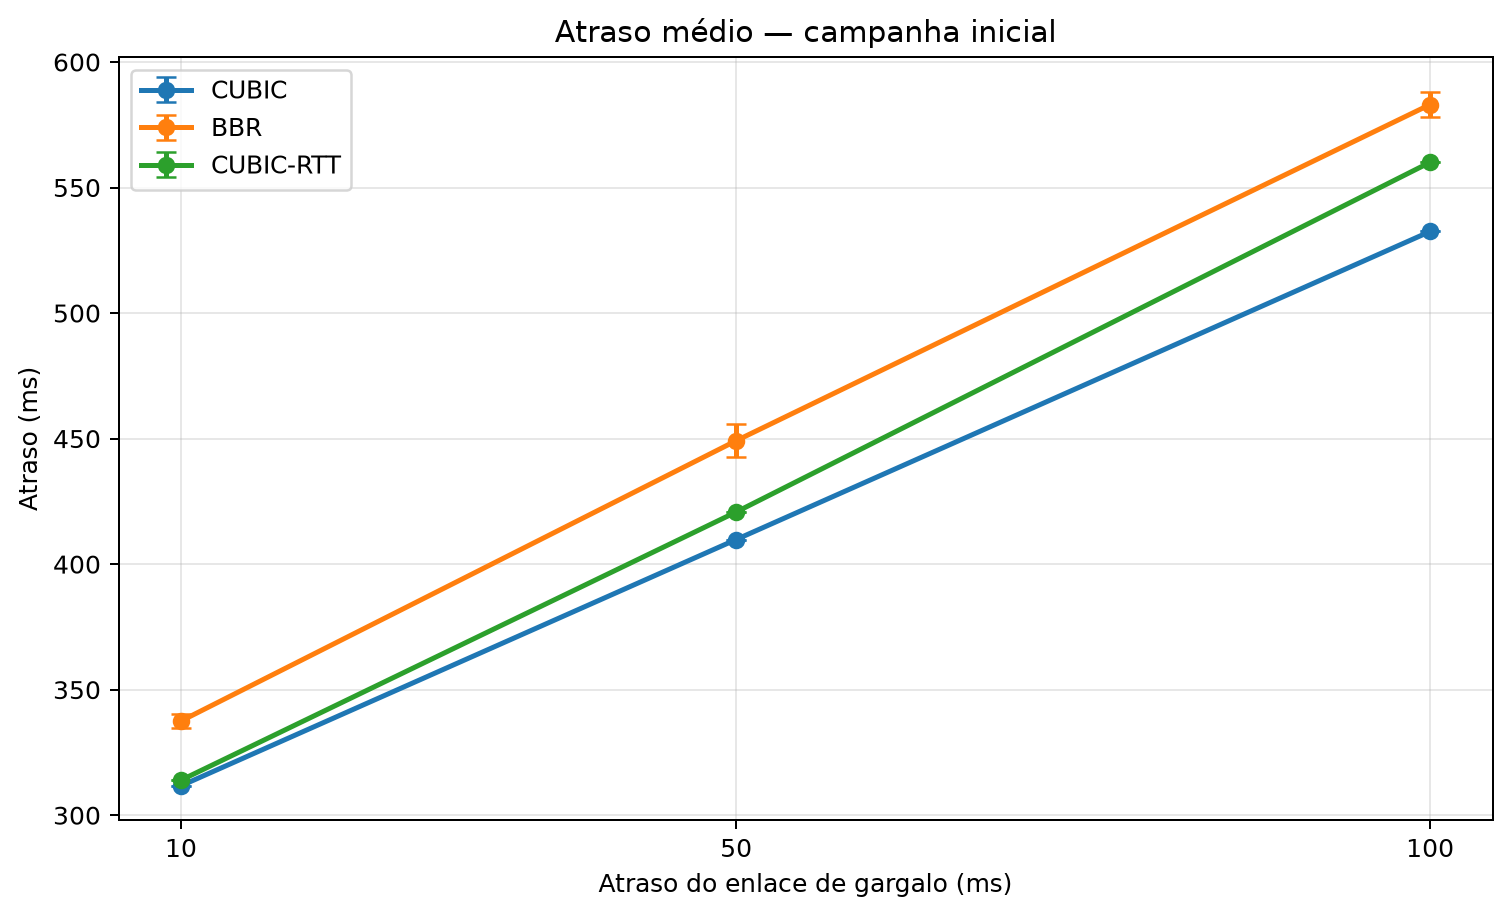
\includegraphics[width=0.88\textwidth]{inicial_delay.png}
\caption{Atraso médio unidirecional na campanha inicial.}
\label{fig:inicial-atraso}
\end{figure}

O gráfico de RTT médio complementa essa leitura, pois apresenta a medida de ida e volta observada pela conexão, distinta do atraso unidirecional do FlowMonitor. As duas métricas não são intercambiáveis: a primeira alimenta a lógica adaptativa do CUBIC-RTT, enquanto a segunda descreve o tempo de entrega dos pacotes em um sentido.

\begin{figure}[htbp]
\centering
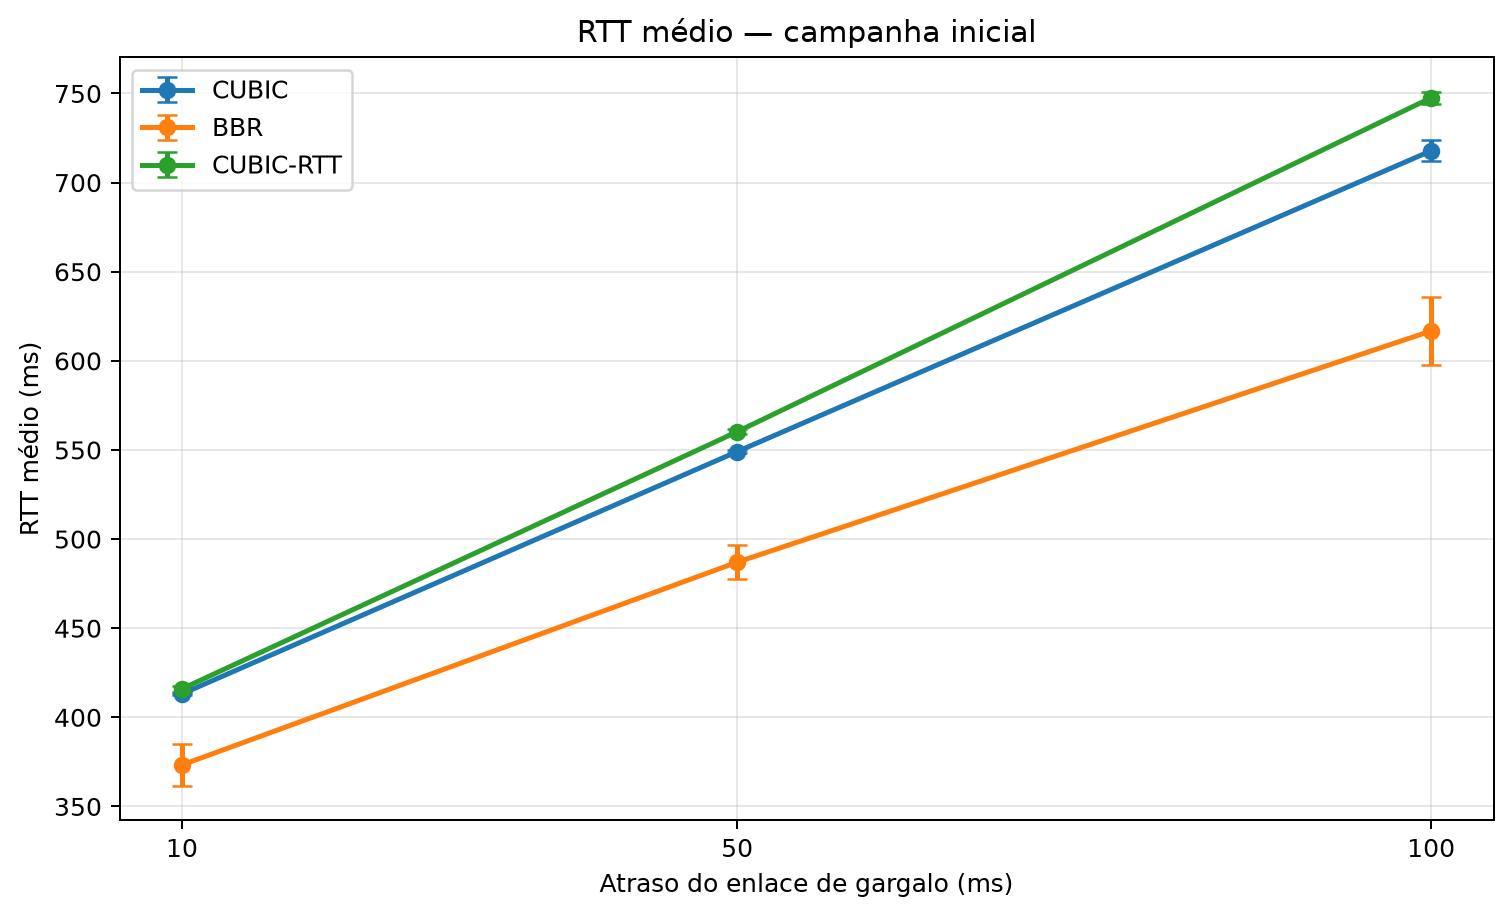
\includegraphics[width=0.88\textwidth]{inicial_rtt.png}
\caption{RTT médio observado na campanha inicial.}
\label{fig:inicial-rtt}
\end{figure}

\subsection{Jitter}

O resultado mais favorável ao CUBIC-RTT na comparação inicial foi o jitter. A proposta registrou 1,610 ms, 1,595 ms e 1,659 ms, enquanto o CUBIC apresentou 1,632 ms, 1,650 ms e 1,718 ms. As reduções foram de aproximadamente 1,3\%, 3,3\% e 3,4\%.

As diferenças absolutas são moderadas, mas mantêm o mesmo sentido nos três atrasos avaliados. O BBR apresentou jitter ainda menor, entre 1,060 ms e 1,190 ms, mas esse resultado ocorreu junto de perdas de pacotes muito superiores às observadas nos dois algoritmos CUBIC.

\begin{figure}[htbp]
\centering
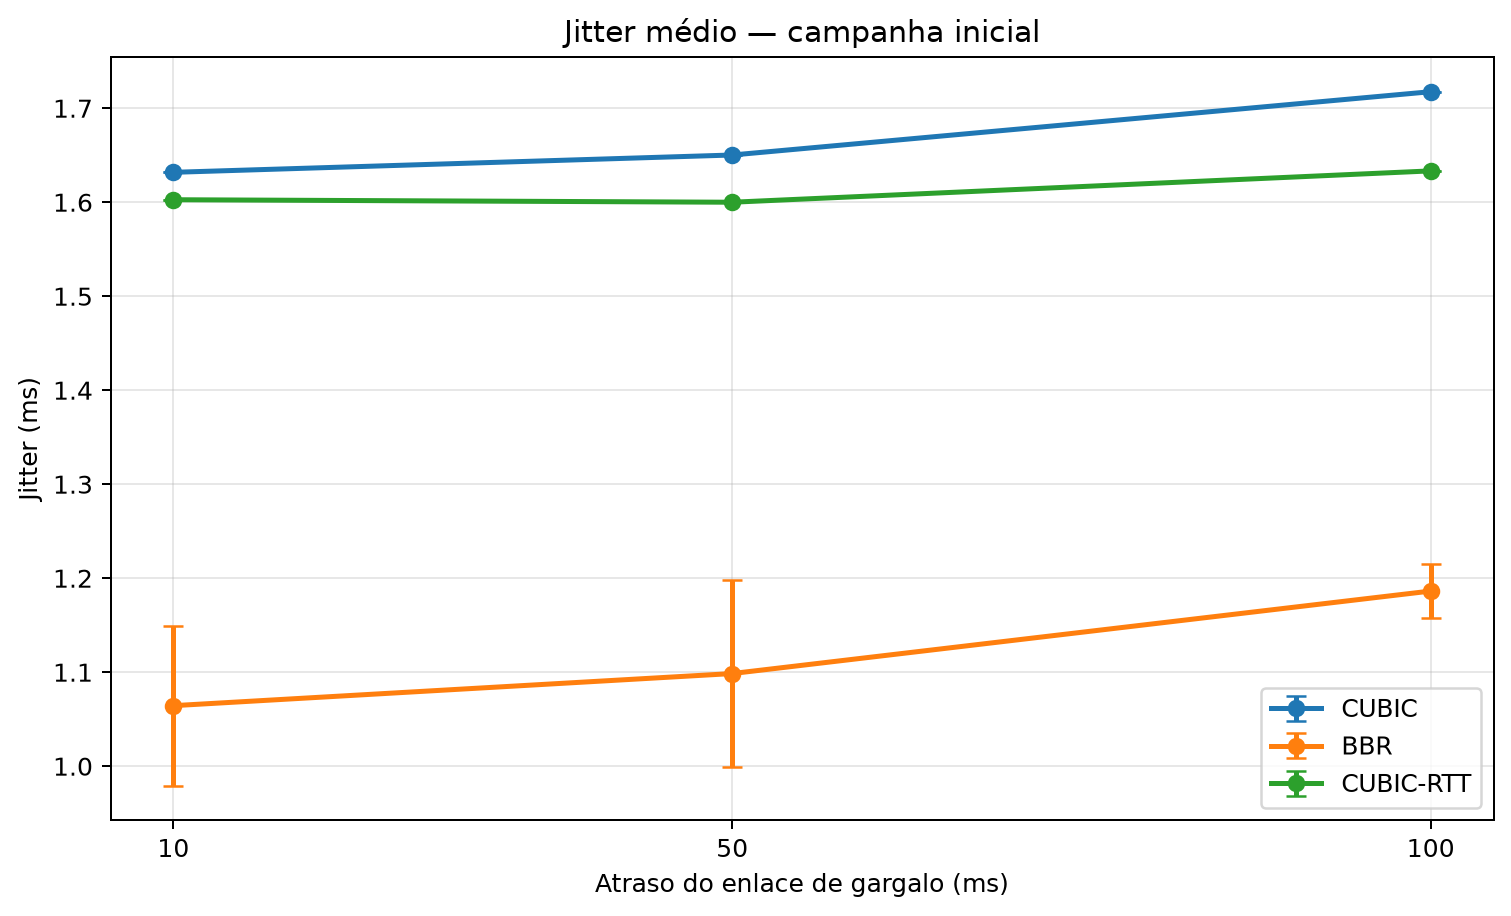
\includegraphics[width=0.88\textwidth]{inicial_jitter.png}
\caption{Jitter médio na campanha inicial.}
\label{fig:inicial-jitter}
\end{figure}

Em resumo, os resultados iniciais indicam que a adaptação pode alterar a regularidade temporal da entrega sem reduzir a vazão agregada. Essa mudança, porém, não veio acompanhada de menor atraso ou menor perda de forma consistente. A primeira campanha sustenta a hipótese de que informações de RTT influenciam o comportamento do CUBIC, mas não demonstra melhoria global em todas as métricas.

\section{Campanha de Robustez e Variação de Parâmetros}

A campanha de robustez reuniu 675 simulações, distribuídas em três cenários de rede, quinze configurações de algoritmo e parâmetros, três atrasos de gargalo e cinco repetições. Foram avaliados o CUBIC original, o BBR e treze configurações do CUBIC-RTT, incluindo a configuração de referência ($\alpha=0{,}25$ e $\gamma=0{,}05$).

Os mapas de calor preservados no projeto permitem examinar em detalhe os cenários \texttt{bw1\_f4} e \texttt{bw2\_f8}. O cenário \texttt{access100} também integrou a matriz de execução e a auditoria estrutural, mas não possui, no conjunto de figuras desta versão, mapas equivalentes que permitam uma discussão numérica com o mesmo nível de detalhe. Por isso, a comparação quantitativa a seguir concentra-se nos dois cenários com resultados gráficos disponíveis.

\subsection{Cenário bw1\_f4: gargalo de 1 Mbps e quatro fluxos}

Nesse cenário, a vazão permaneceu próxima de 0,99 Mbps para o CUBIC e para todas as configurações CUBIC-RTT, independentemente do atraso do gargalo. Isso indica que a capacidade disponível foi praticamente toda utilizada e que a variação de $\alpha$ e $\gamma$ não produziu diferenças relevantes na vazão agregada.

As diferenças aparecem com maior clareza nas demais métricas. Com 100 ms de atraso, o CUBIC apresentou perda de 3,52\%, atraso médio de 652,12 ms, jitter de 3,57 ms e índice de Jain de 0,97. A configuração de referência do CUBIC-RTT apresentou, no mesmo cenário, perda de 4,11\%, atraso de 661,68 ms, jitter de 3,53 ms e índice de Jain de 0,99. Houve, então, pequena redução de jitter e melhor distribuição entre os fluxos, mas com aumento da perda e do atraso médio.

A variação dos coeficientes mostra que não existe uma combinação que minimize simultaneamente todas as métricas. Por exemplo, com 100 ms, a configuração $\alpha=0{,}50$ e $\gamma=0{,}025$ apresentou atraso médio de 633,86 ms, abaixo dos 652,12 ms do CUBIC. Entretanto, sua perda foi de 4,75\%, superior aos 3,52\% do algoritmo original, e o jitter chegou a 3,69 ms. Já a configuração $\alpha=0{,}10$ e $\gamma=0$ obteve atraso de 641,33 ms e perda de 3,83\%, combinando menor atraso que o CUBIC com perda um pouco maior.

O BBR manteve vazão próxima de 0,97 Mbps, mas apresentou perdas de 4,30\%, 17,70\% e 18,57\% nos três atrasos. Seu índice de Jain caiu para 0,65 em 50 ms e 0,82 em 100 ms. Novamente, esses números caracterizam o cenário simulado, não uma propriedade universal do BBR.

\subsection{Cenário bw2\_f8: gargalo de 2 Mbps e oito fluxos}

Com oito fluxos concorrentes e gargalo de 2 Mbps, a vazão também permaneceu próxima da capacidade disponível. CUBIC e CUBIC-RTT registraram aproximadamente 1,98 Mbps em 10 ms e 1,97 Mbps em 50 ms e 100 ms. A mudança dos coeficientes teve pouco efeito sobre essa métrica agregada.

A diferença entre as configurações voltou a aparecer no atraso, no jitter, na perda e na justiça. Com 100 ms, o CUBIC apresentou atraso médio de 548,06 ms, jitter de 2,19 ms, perda de 2,76\% e índice de Jain de 0,96. A configuração de referência do CUBIC-RTT apresentou atraso de 556,43 ms, jitter de 2,18 ms, perda de 3,21\% e índice de Jain de 0,94. Nesse caso, a pequena redução de jitter veio acompanhada de aumento do atraso e da perda e de uma distribuição um pouco menos equilibrada.

Algumas combinações produziram compromissos diferentes. A configuração $\alpha=0{,}10$ e $\gamma=0{,}10$, por exemplo, reduziu o jitter para 1,90 ms, 1,87 ms e 1,93 ms nos três atrasos, abaixo dos valores do CUBIC. Em contrapartida, com 100 ms, seu atraso médio foi de 578,82 ms e a perda foi de 3,11\%, ambos superiores aos do algoritmo original. Por outro lado, configurações com $\gamma=0$ chegaram a apresentar atraso médio menor em 100 ms, mas sem manter a mesma vantagem em jitter e perda.

O BBR apresentou perdas entre 20,15\% e 21,48\% e índices de Jain entre 0,46 e 0,74. Embora sua vazão tenha permanecido próxima de 1,93--1,95 Mbps, a distribuição entre os oito fluxos foi consideravelmente menos equilibrada nesse cenário específico.

\subsection{Influência dos coeficientes \texorpdfstring{$\alpha$ e $\gamma$}{alpha e gamma}}

Os mapas de calor mostram que a influência dos coeficientes depende do cenário e da métrica observada. O coeficiente $\alpha$ altera a intensidade da adaptação do fator cúbico $C$, afetando o crescimento da janela. O coeficiente $\gamma$ modula a alteração de $\beta$ após a perda. Como os dois mecanismos atuam em momentos diferentes do controle de congestionamento, seus efeitos não precisam aparecer simultaneamente nem na mesma direção em todas as métricas.

De forma geral, a vazão agregada permaneceu próxima ao limite do gargalo em quase todas as configurações. Isso significa que a comparação entre parâmetros é mais informativa quando se observam atraso, jitter, perda e justiça. Em algumas condições, determinadas combinações reduziram o atraso ou o jitter, mas aumentaram a perda de pacotes; em outras, melhoraram o índice de Jain sem oferecer vantagem de vazão. A configuração de referência, portanto, deve ser entendida como um ponto de partida para a avaliação, e não como uma escolha ótima para todos os cenários.

A campanha de robustez reforça a conclusão da comparação inicial: a adaptação baseada em RTT modifica o comportamento do CUBIC e pode favorecer uma métrica em determinadas condições, mas o efeito não é uniforme. Não foi identificada uma combinação de $\alpha$ e $\gamma$ que dominasse o CUBIC original em vazão, atraso, jitter, perda e justiça ao mesmo tempo.

\section{Coexistência entre Fluxos CUBIC e CUBIC-RTT}

A campanha de coexistência avalia uma questão diferente das comparações anteriores: não apenas como cada algoritmo se comporta isoladamente, mas como os dois disputam a mesma capacidade de transmissão. Foram utilizados oito fluxos simultâneos, quatro CUBIC e quatro CUBIC-RTT, com a mesma configuração de referência da proposta ($\alpha=0{,}25$ e $\gamma=0{,}05$). Os enlaces de acesso foram distribuídos em pares com atrasos de 10 ms, 30 ms, 60 ms e 90 ms, enquanto o gargalo de 10 Mbps foi avaliado com atrasos de 10 ms, 50 ms e 100 ms.

A Tabela~\ref{tab:coexistencia} apresenta a vazão média por fluxo, o atraso médio, o jitter e a perda de cada grupo. Para cada repetição, foram calculadas as médias dos quatro fluxos pertencentes ao mesmo algoritmo; em seguida, foram calculadas as médias das cinco repetições. A perda foi consolidada pela razão entre pacotes perdidos e pacotes transmitidos.

\begin{table}[htbp]
\centering
\caption{Resultados médios da campanha de coexistência}
\label{tab:coexistencia}
\small
\resizebox{\textwidth}{!}{
\begin{tabular}{c l r r r r}
\toprule
\textbf{Atraso do gargalo} & \textbf{Algoritmo} & \textbf{Vazão por fluxo (Mbps)} & \textbf{Perda (\%)} & \textbf{Atraso médio (ms)} & \textbf{Jitter (ms)} \\
\midrule
10 ms & CUBIC & 1,2492 & 0,2465 & 450,008 & 0,6100 \\
10 ms & CUBIC-RTT & 1,2345 & 0,2416 & 449,700 & 0,6131 \\
\midrule
50 ms & CUBIC & 1,2068 & 0,3229 & 552,776 & 0,6487 \\
50 ms & CUBIC-RTT & 1,2757 & 0,3177 & 552,603 & 0,6380 \\
\midrule
100 ms & CUBIC & 1,1070 & 0,5070 & 678,778 & 0,7060 \\
100 ms & CUBIC-RTT & 1,3746 & 0,4590 & 678,291 & 0,6556 \\
\bottomrule
\end{tabular}}
\end{table}

\subsection{Vazão: redistribuição da capacidade entre os algoritmos}

Com atraso de gargalo de 10 ms, a vazão média por fluxo CUBIC foi de 1,2492 Mbps, ligeiramente superior aos 1,2345 Mbps do CUBIC-RTT. A diferença representa aproximadamente 1,2\%. Em 50 ms, a relação se inverteu: o CUBIC-RTT alcançou 1,2757 Mbps por fluxo, contra 1,2068 Mbps do CUBIC, uma vantagem de aproximadamente 5,7\%.

A diferença ficou mais evidente em 100 ms. O CUBIC-RTT atingiu 1,3746 Mbps por fluxo, enquanto o CUBIC caiu para 1,1070 Mbps, o que representa uma vantagem de aproximadamente 24,2\% para a variante adaptativa. Como cada algoritmo possui quatro fluxos, a vazão total da rede permaneceu próxima de 9,93 Mbps nos três cenários. Na prática, o aumento da vazão do CUBIC-RTT não representa um crescimento equivalente da capacidade total utilizada: representa principalmente uma redistribuição da banda em favor dos fluxos que executam a proposta.

A participação do CUBIC-RTT na vazão total passou de aproximadamente 49,7\% em 10 ms para 51,4\% em 50 ms e 55,4\% em 100 ms. Esse resultado é central para a avaliação da hipótese: a adaptação pode manter a utilização do gargalo e, ao mesmo tempo, tornar o CUBIC-RTT mais competitivo que o CUBIC original quando os atrasos aumentam. Isso também significa que a proposta não é neutra em relação a fluxos CUBIC concorrentes.

\begin{figure}[htbp]
\centering
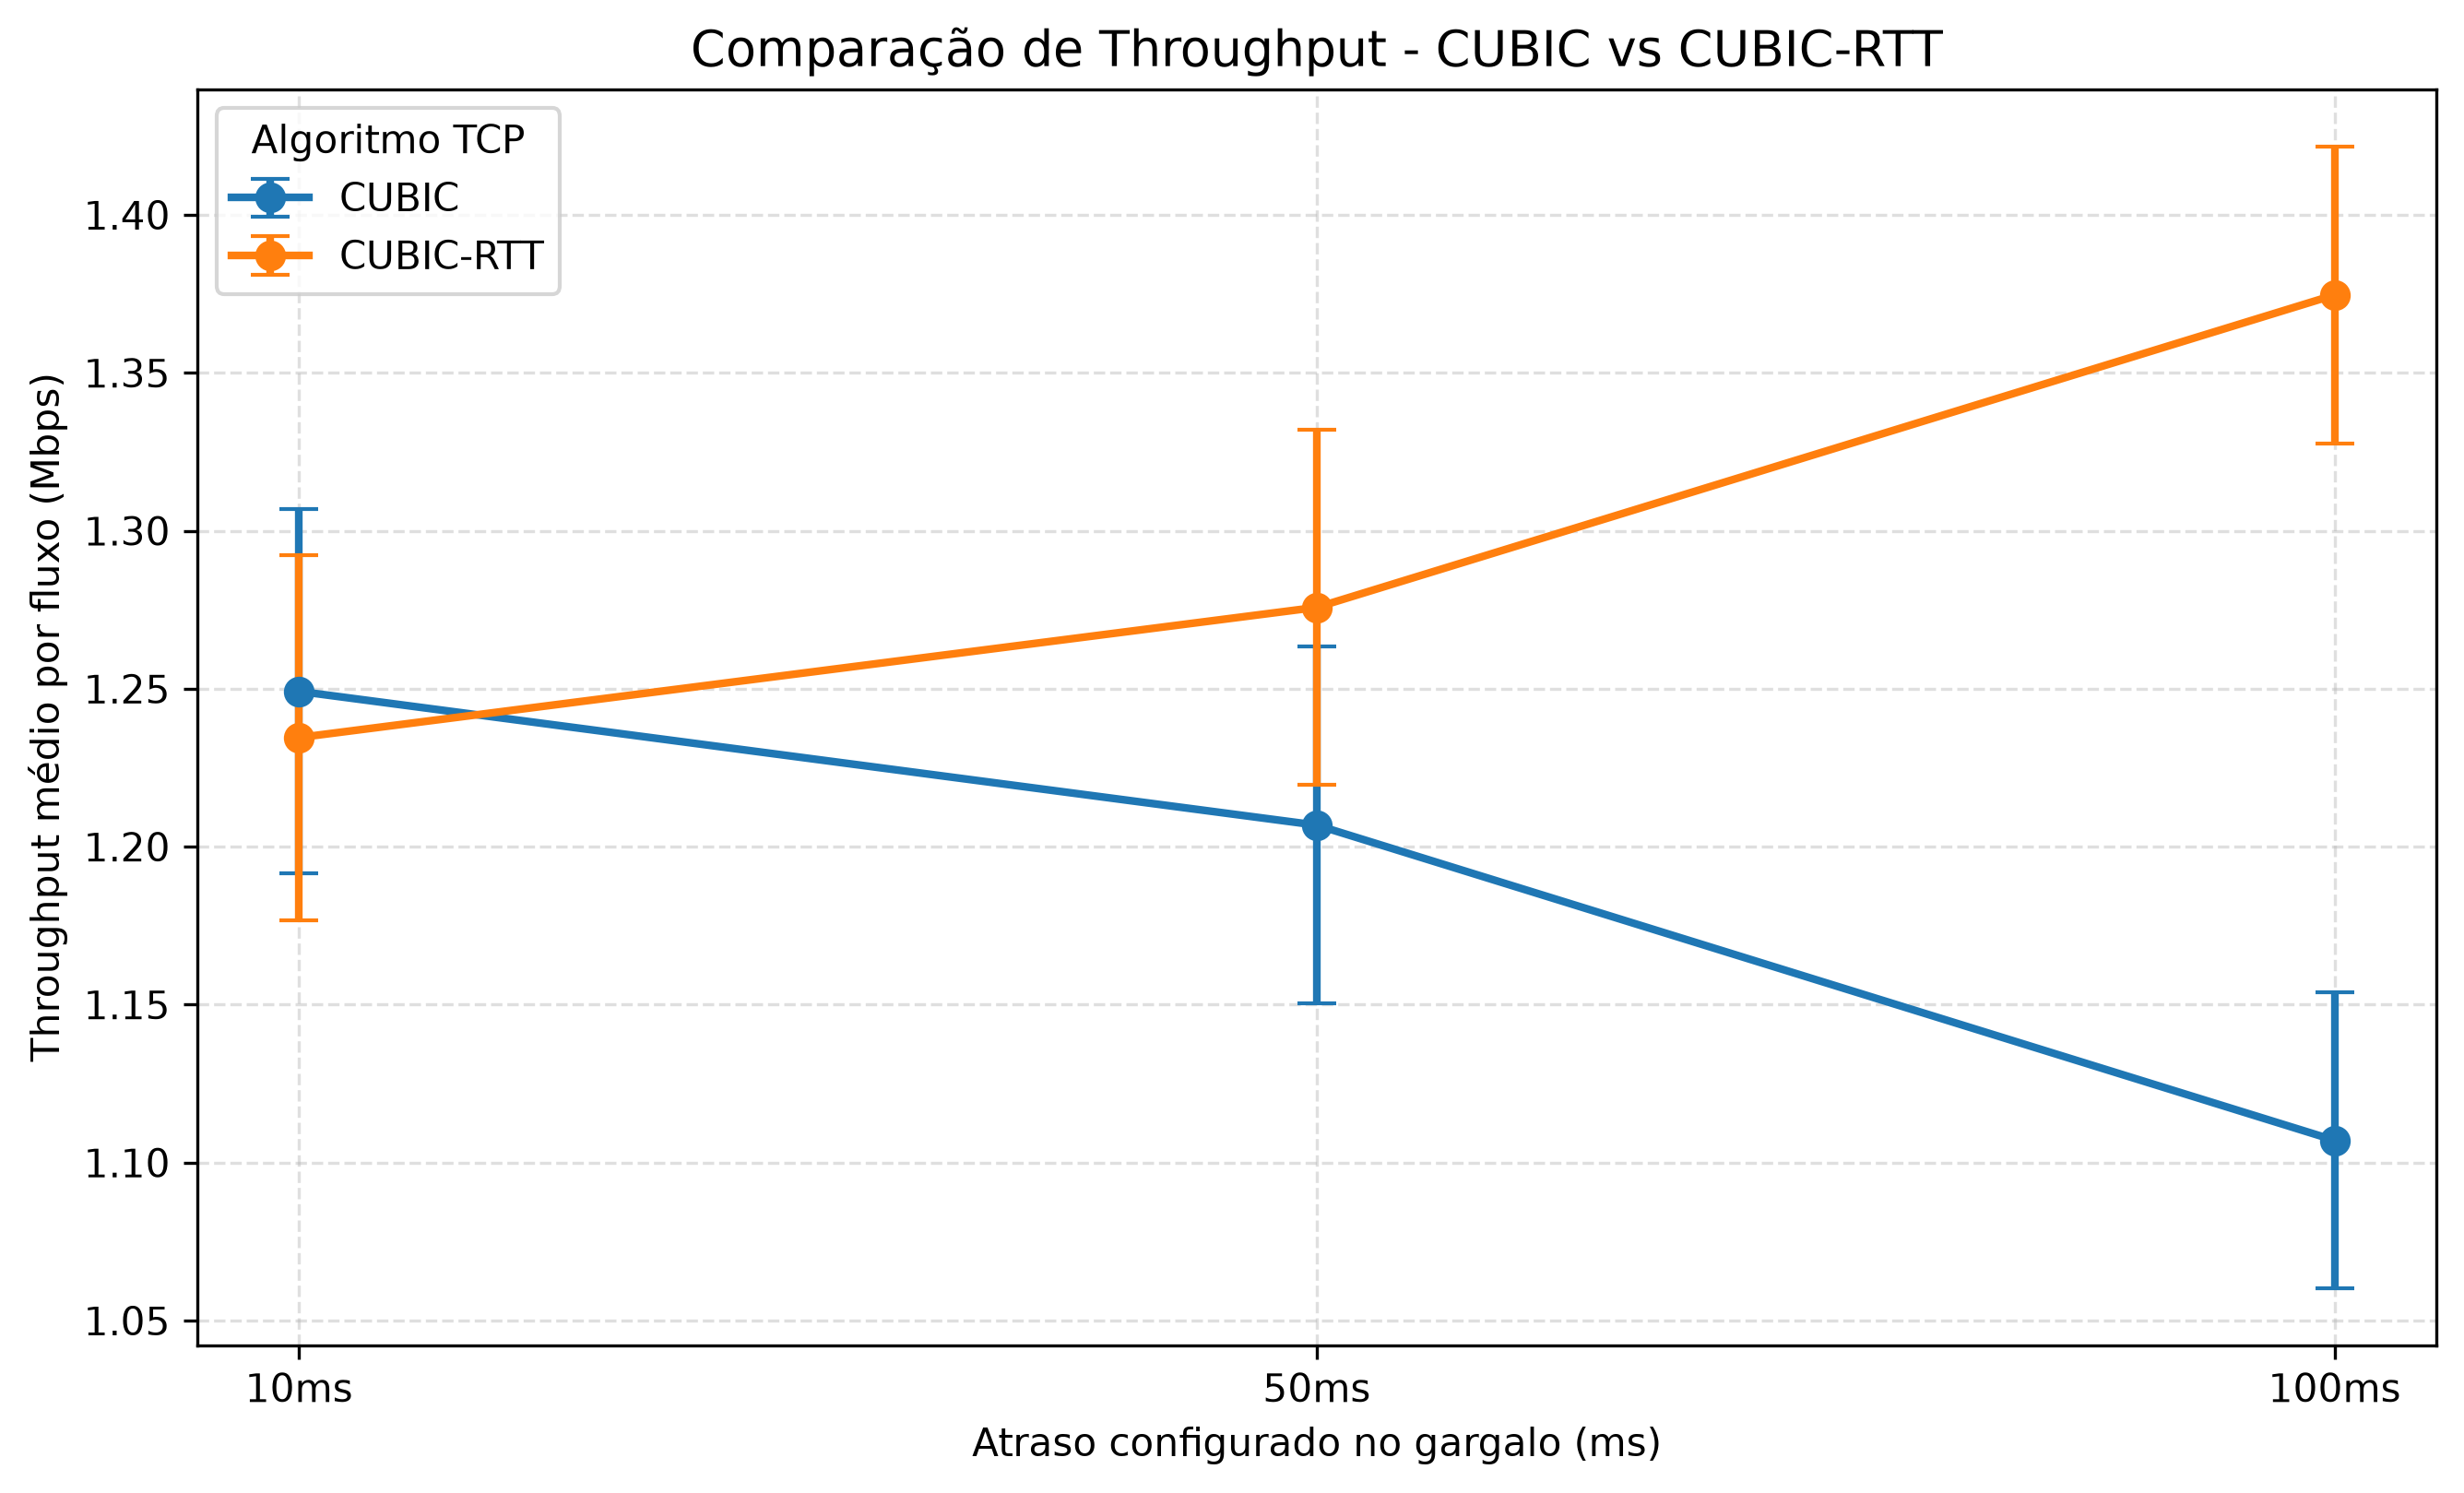
\includegraphics[width=0.90\textwidth]{01_throughput.png}
\caption{Vazão média por fluxo na campanha de coexistência.}
\label{fig:coex-throughput}
\end{figure}

\subsection{Atraso médio}

O atraso médio dos dois grupos permaneceu praticamente igual em todos os cenários. Em 10 ms, a diferença foi de aproximadamente 0,31 ms; em 50 ms, 0,17 ms; e em 100 ms, 0,49 ms. Essas diferenças são muito pequenas quando comparadas aos valores absolutos, que cresceram de aproximadamente 450 ms para 678 ms à medida que o atraso do gargalo aumentou.

Na prática, o ganho de vazão do CUBIC-RTT em 50 ms e 100 ms não foi acompanhado por uma redução expressiva do atraso médio. Os dois algoritmos experimentaram condições de atraso muito próximas, embora tenham obtido parcelas diferentes da vazão disponível.

\begin{figure}[htbp]
\centering
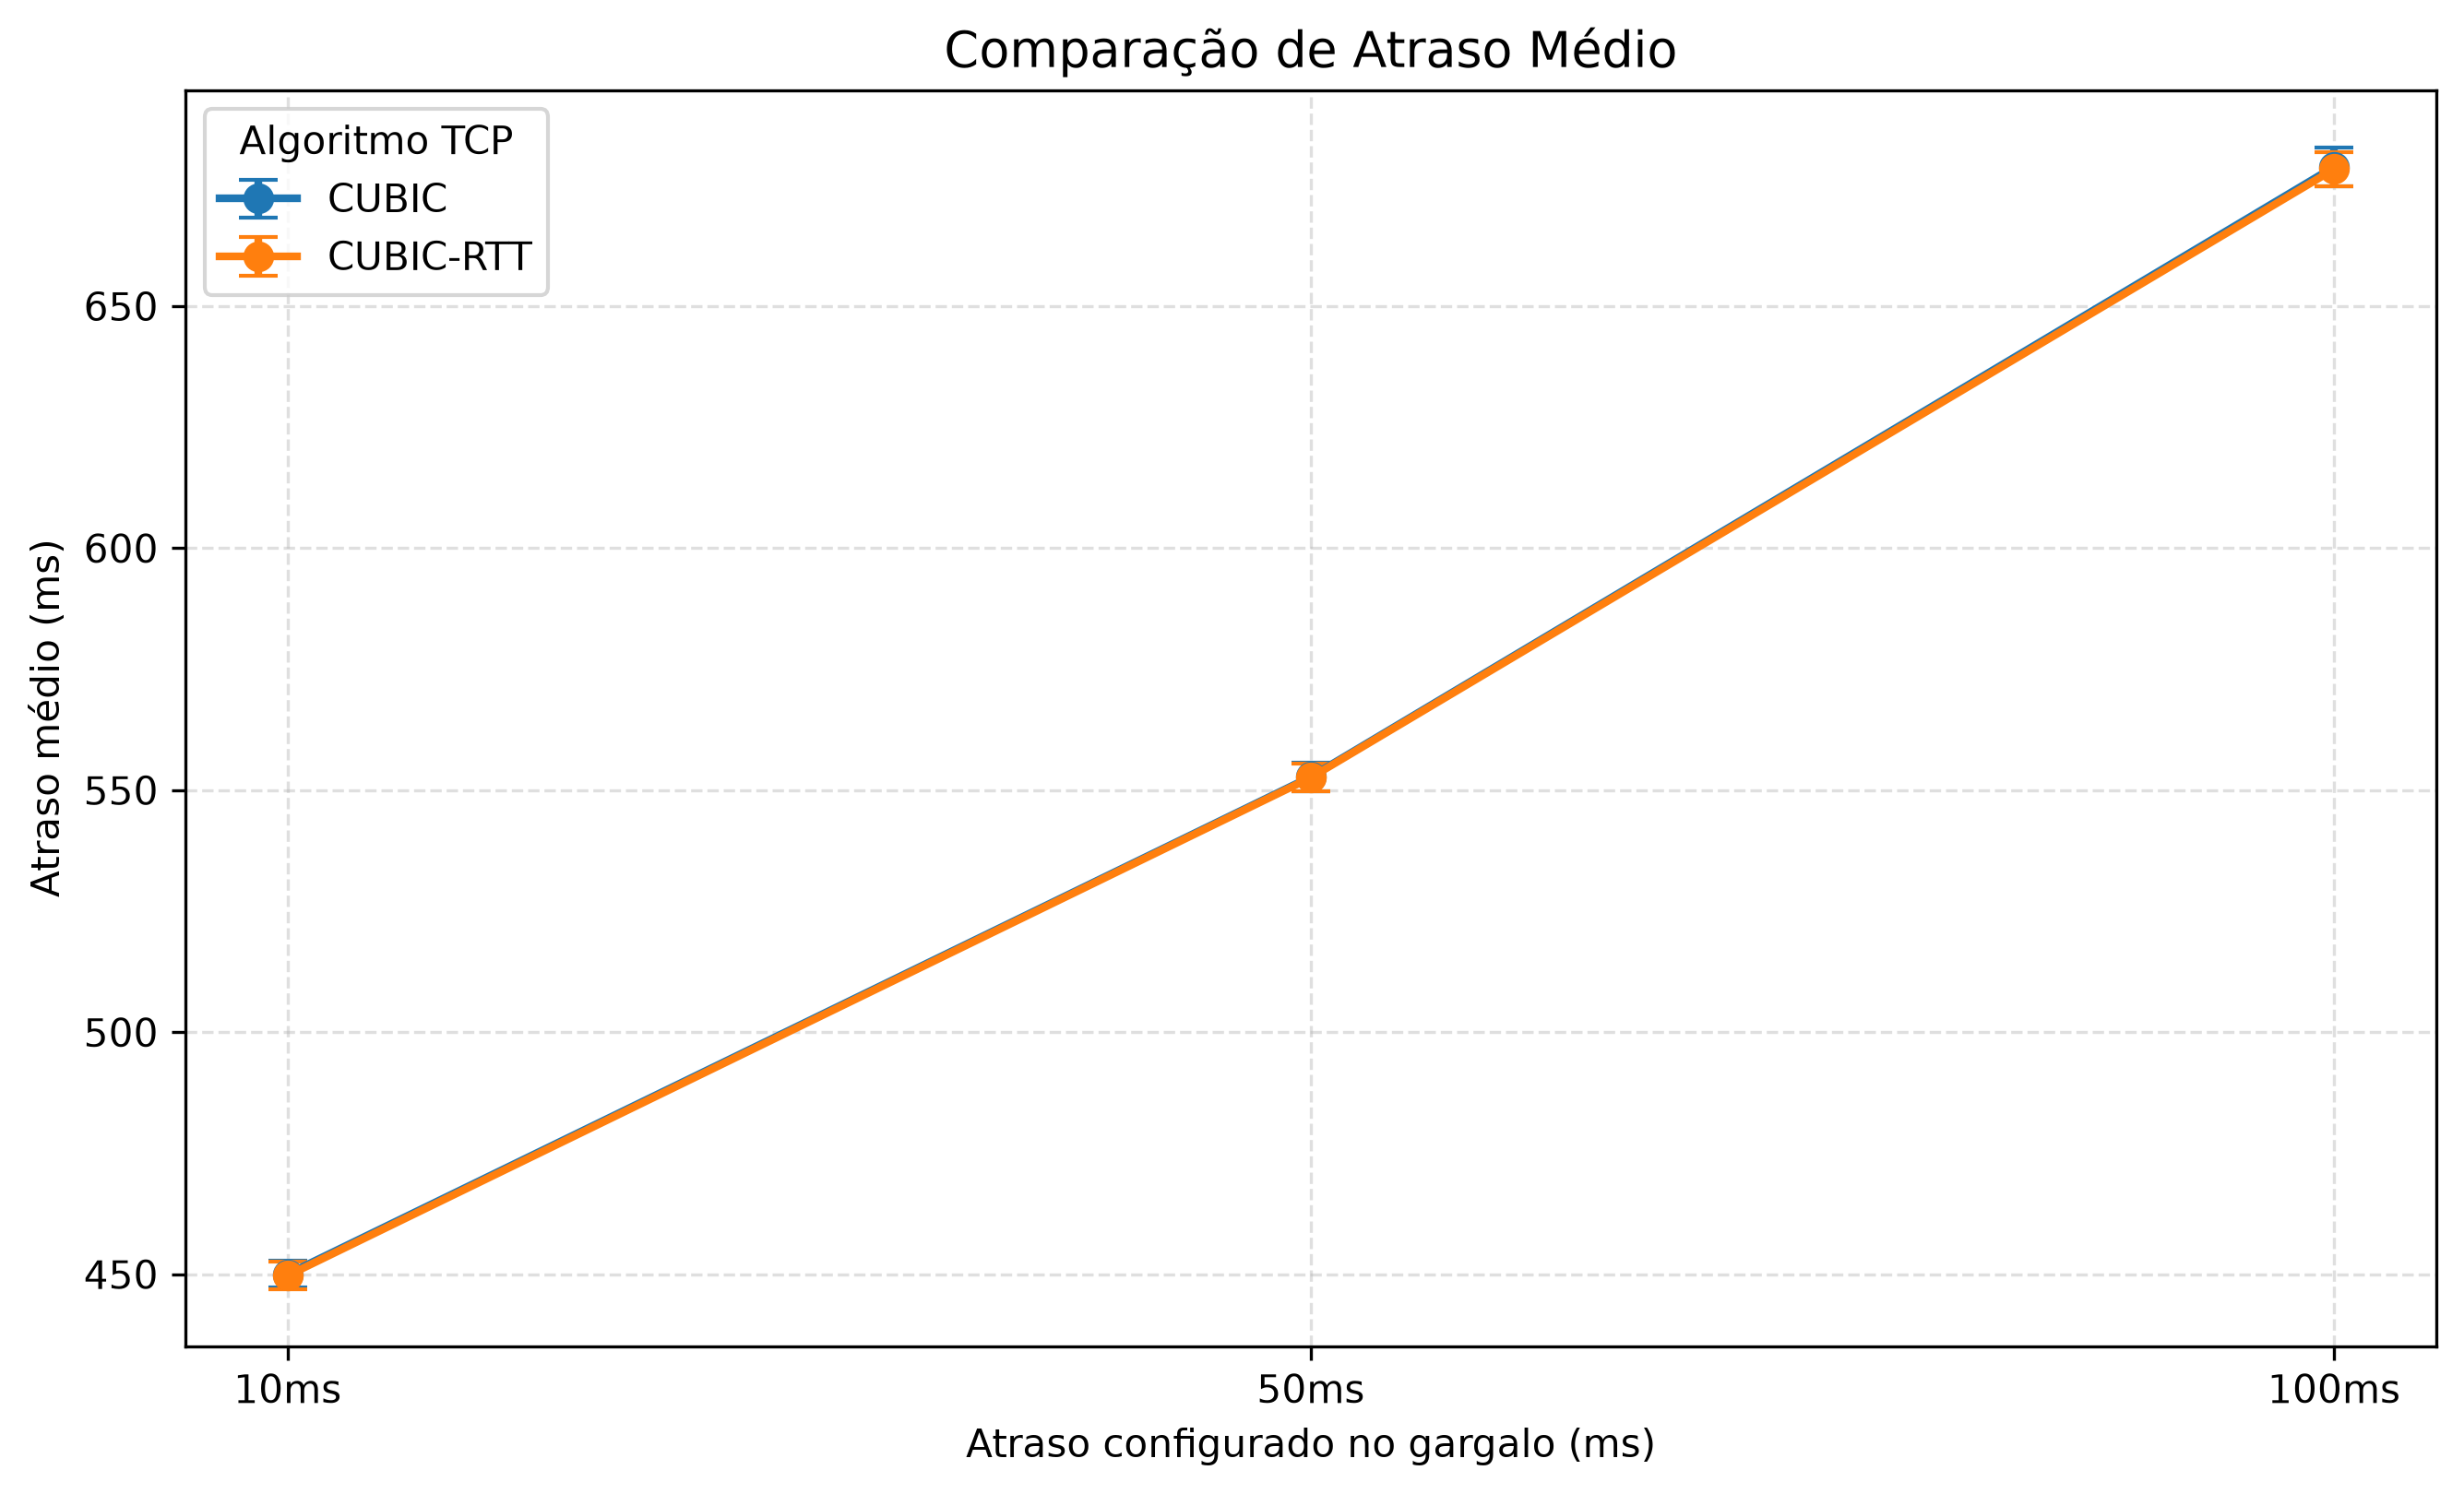
\includegraphics[width=0.90\textwidth]{02_atraso_medio.png}
\caption{Atraso médio dos fluxos na campanha de coexistência.}
\label{fig:coex-atraso}
\end{figure}

\subsection{Jitter e perda de pacotes}

No cenário de 10 ms, o jitter dos dois algoritmos foi praticamente igual: 0,6100 ms para CUBIC e 0,6131 ms para CUBIC-RTT. Em 50 ms, o jitter do CUBIC-RTT foi menor, 0,6380 ms contra 0,6487 ms. Em 100 ms, a diferença aumentou: 0,6556 ms para a proposta e 0,7060 ms para o CUBIC, uma redução aproximada de 7,1\%.

A perda de pacotes também foi ligeiramente menor para o CUBIC-RTT nos três atrasos. Em 10 ms, os valores foram 0,2416\% e 0,2465\%; em 50 ms, 0,3177\% e 0,3229\%; e em 100 ms, 0,4590\% e 0,5070\%. A diferença mais perceptível ocorreu no maior atraso, em que a perda do CUBIC-RTT ficou aproximadamente 9,5\% abaixo da observada no CUBIC.

\begin{figure}[htbp]
\centering
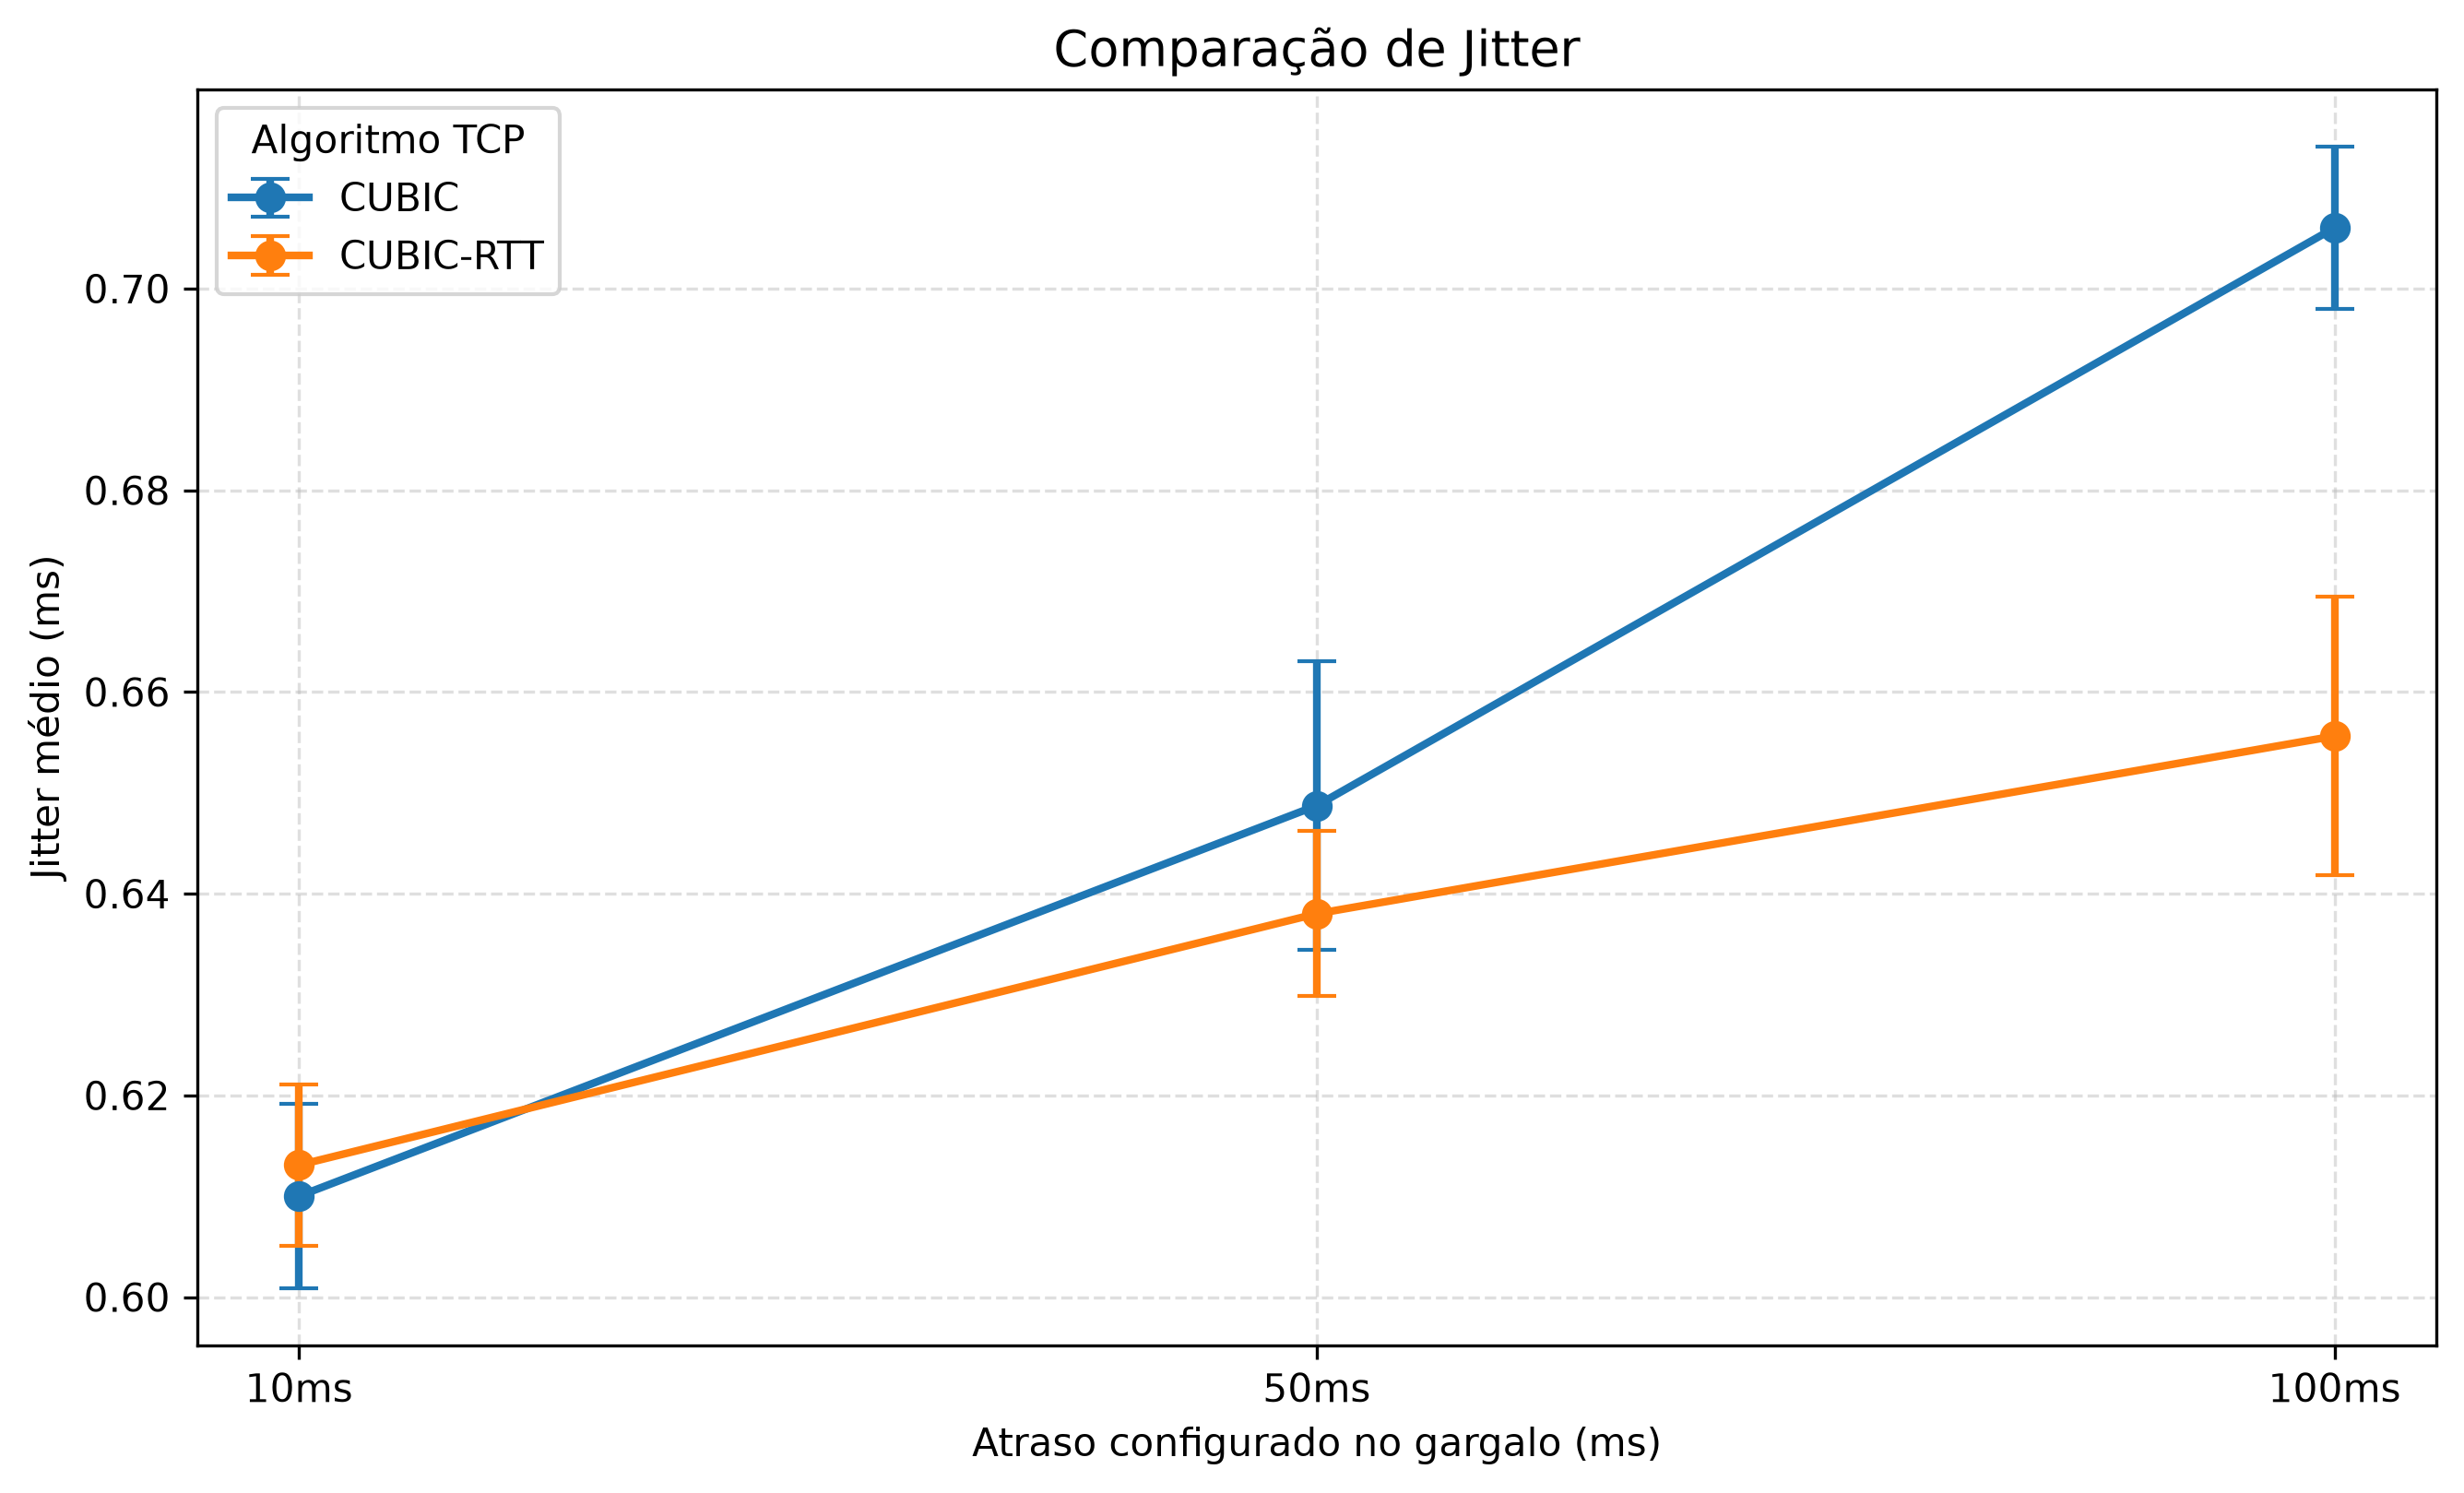
\includegraphics[width=0.90\textwidth]{03_jitter.png}
\caption{Jitter médio na campanha de coexistência.}
\label{fig:coex-jitter}
\end{figure}

\begin{figure}[htbp]
\centering
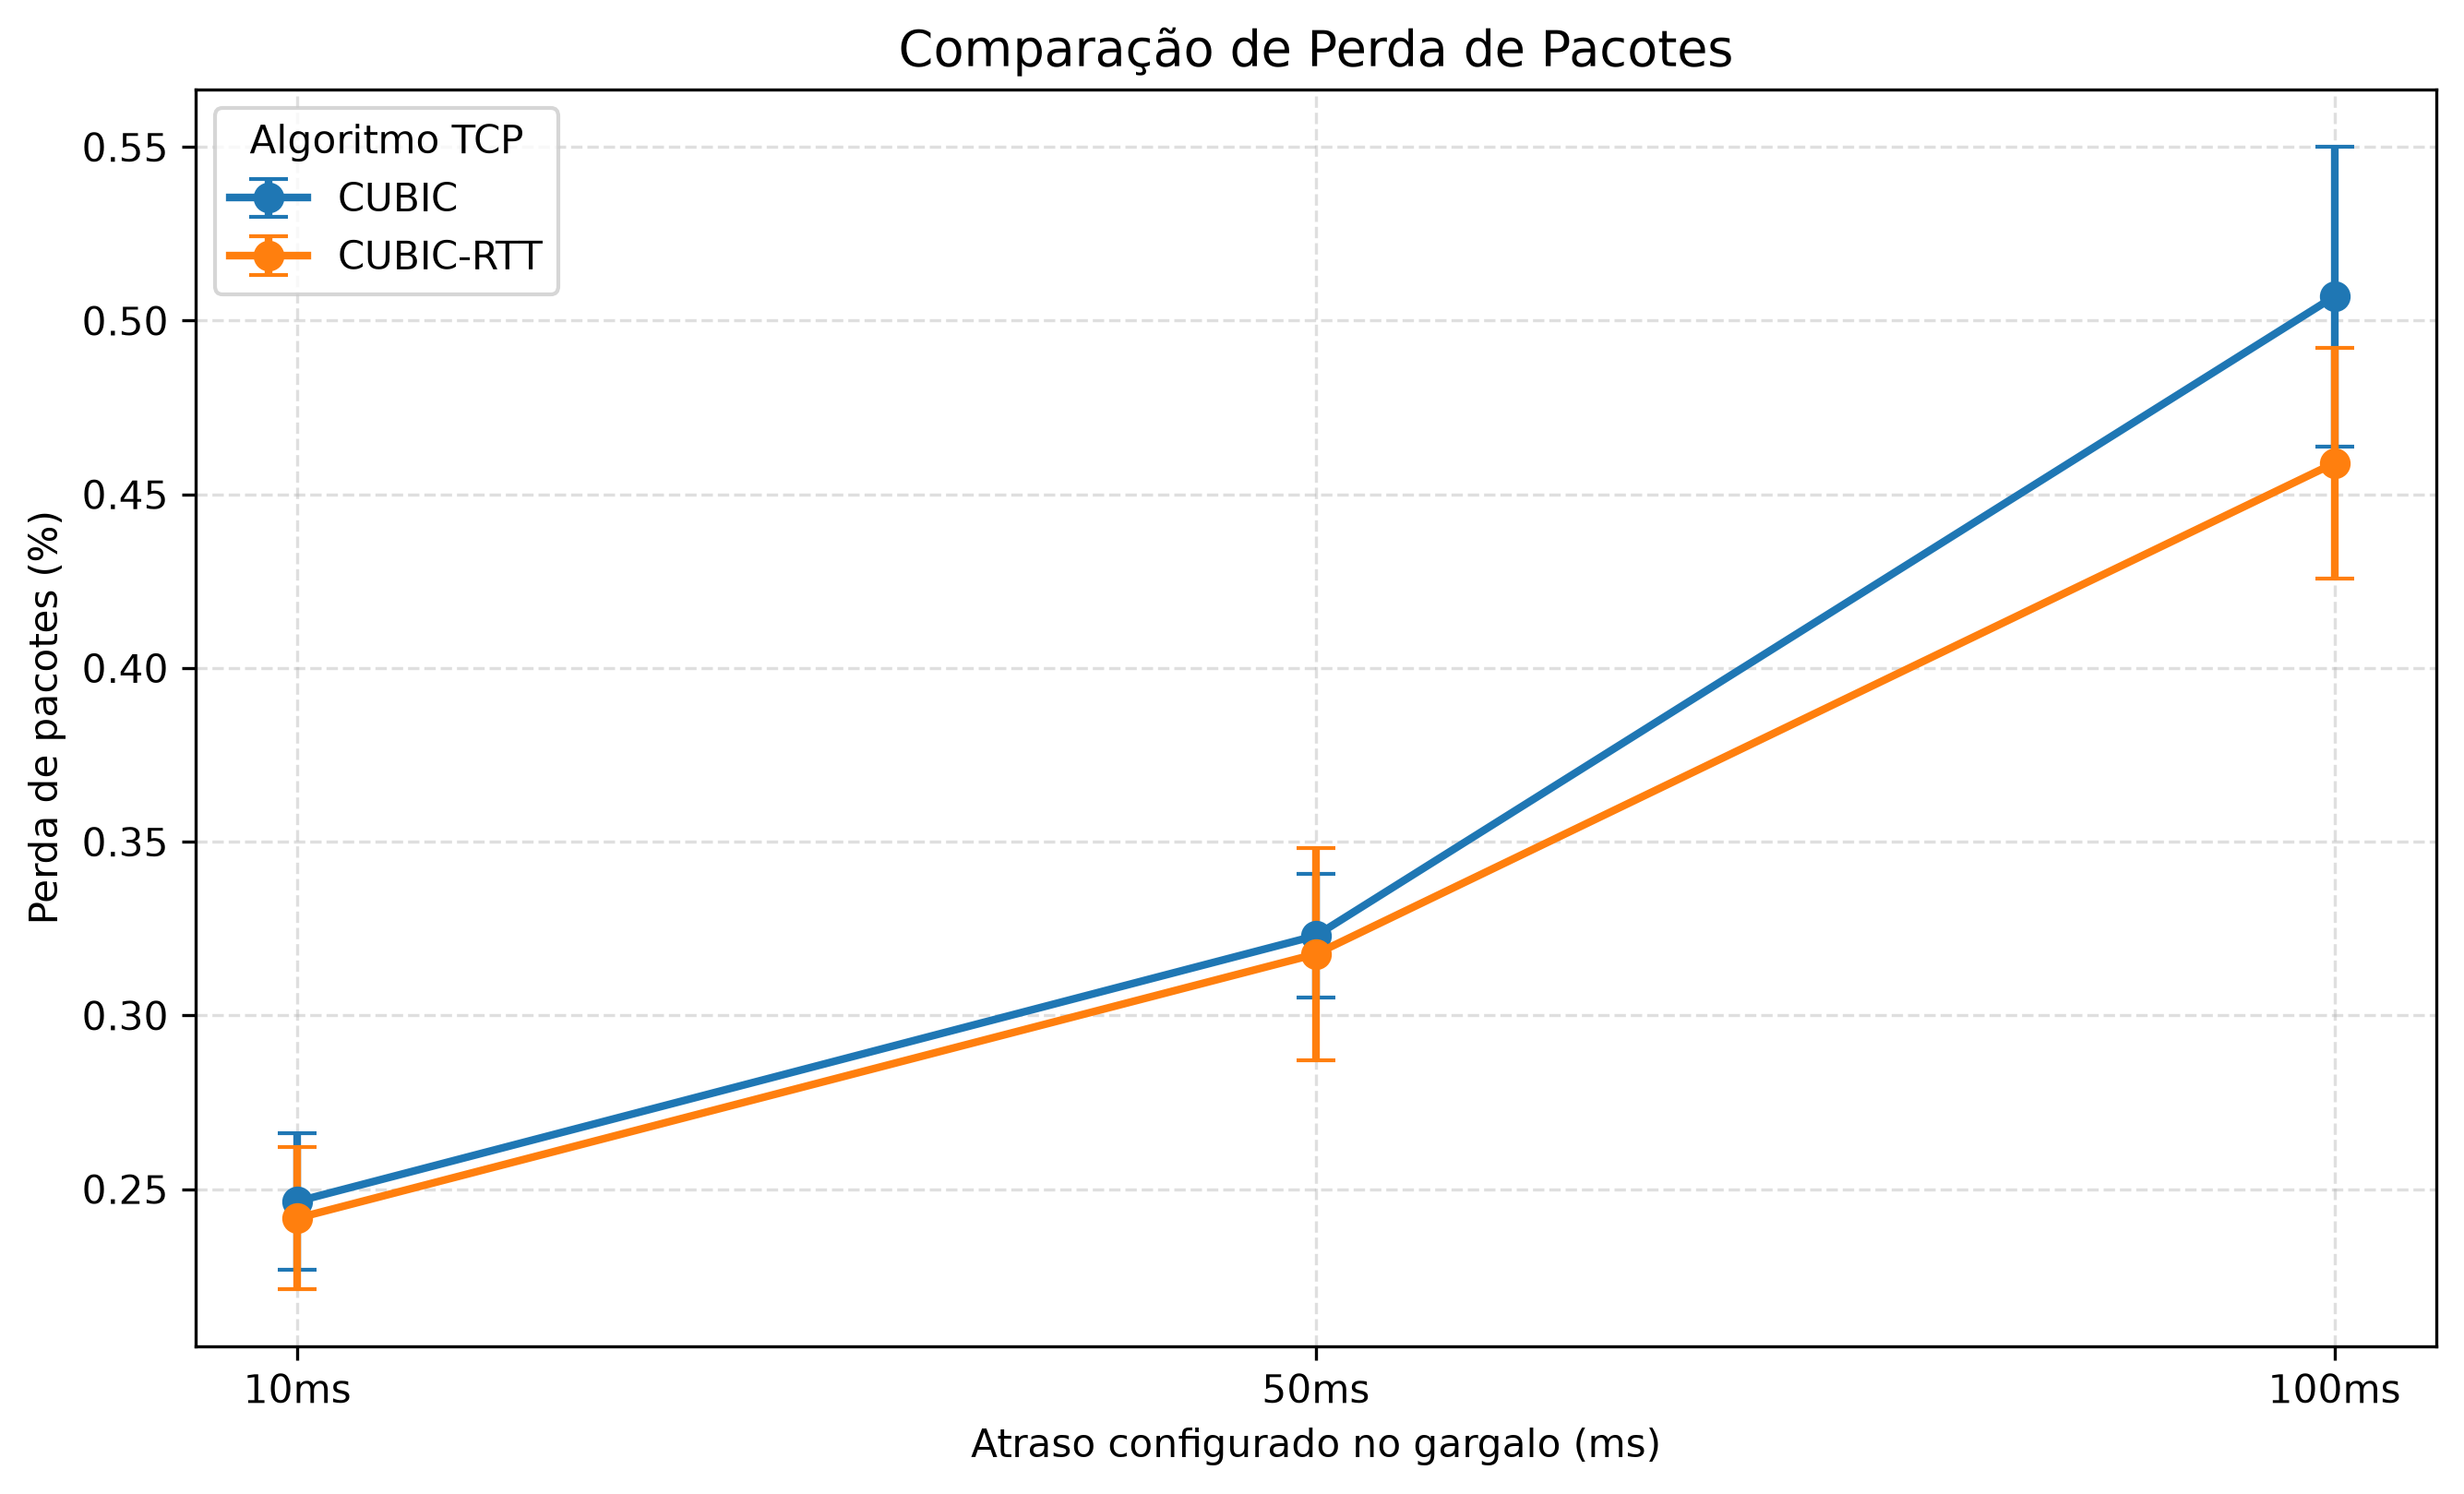
\includegraphics[width=0.90\textwidth]{04_packet_loss.png}
\caption{Taxa de perda de pacotes na campanha de coexistência.}
\label{fig:coex-perda}
\end{figure}

\subsection{Interpretação da coexistência}

A campanha mostra que o CUBIC-RTT consegue coexistir com o CUBIC sem derrubar a vazão total da rede e sem diferença expressiva no atraso médio. Coexistir, no entanto, não significa dividir os recursos igualmente: à medida que o atraso do gargalo aumentou, os fluxos CUBIC-RTT ficaram com uma fatia cada vez maior da capacidade, enquanto a vazão média dos fluxos CUBIC diminuiu.

Esse resultado sugere que a adaptação baseada em RTT dá à variante uma vantagem competitiva em cenários de maior atraso. A vantagem veio acompanhada de jitter e perda ligeiramente menores, mas não de uma redução significativa do atraso médio. Por isso, a proposta não deve ser descrita como uma simples melhoria de desempenho: ela muda a relação competitiva entre os algoritmos e pode favorecer quem a utiliza.

O ponto é relevante para a hipótese do trabalho. A informação de RTT mostrou-se útil para modificar a dinâmica do CUBIC, mas o experimento também deixa claro que uma adaptação vantajosa para os fluxos modificados pode reduzir a parcela de banda dos fluxos que continuam usando o algoritmo original. A avaliação da justiça entre algoritmos precisa, portanto, caminhar junto com a avaliação do desempenho individual.

\section{Análise das Variáveis Internas do TCP}

Os rastros de CWND, SSThresh, RTT, RTO e quantidade de dados em trânsito foram utilizados para observar a dinâmica das conexões ao longo das simulações. A auditoria estrutural confirmou 3.780 arquivos de CWND e 3.780 de SSThresh nas duas primeiras campanhas, sem pares ausentes, erros ou avisos.

Os gráficos temporais preservados para a campanha de coexistência mostram a evolução da janela de congestionamento e do RTT dos oito fluxos nos três atrasos de gargalo. As curvas apresentam fases iniciais de crescimento, seguidas de oscilações associadas à operação do controle de congestionamento. Com o aumento do atraso, a escala temporal do RTT se desloca para valores maiores, enquanto a janela continua apresentando variações ao longo da execução.

Esses rastros ajudam a interpretar as métricas agregadas, mas não devem ser usados isoladamente para afirmar que um algoritmo é melhor. Sua principal utilidade é permitir relacionar a evolução da janela e do RTT com as diferenças de vazão, jitter e perda observadas no FlowMonitor. Os gráficos representativos são reunidos no Apêndice~\ref{ap:traces}.

\section{Discussão Geral}

As três campanhas mostram aspectos complementares da proposta. Na comparação inicial, o CUBIC-RTT manteve a vazão agregada próxima à do CUBIC e reduziu moderadamente o jitter, mas apresentou atraso médio maior e perda ligeiramente superior nos cenários de maior atraso. Na campanha de robustez, a vazão permaneceu próxima da capacidade do gargalo, enquanto as demais métricas variaram de acordo com o cenário e com os valores de $\alpha$ e $\gamma$. Não houve uma configuração que apresentasse o melhor resultado em todas as métricas.

A campanha de coexistência acrescentou um resultado importante: quando CUBIC e CUBIC-RTT compartilham o mesmo gargalo, a variante adaptativa pode obter uma parcela maior da vazão, especialmente quando o atraso do gargalo aumenta. Esse ganho não elevou a vazão total da rede, que permaneceu próxima de 10 Mbps; ele alterou a distribuição da capacidade entre os grupos de fluxos.

Em relação à hipótese de partida, os experimentos sustentam que informações de RTT podem ser incorporadas à estrutura do CUBIC e modificar seu comportamento. Já a expectativa de que essa alteração produza, em qualquer cenário, menor atraso, maior justiça e manutenção integral do desempenho dos fluxos concorrentes não foi confirmada. O resultado mais adequado é considerar o CUBIC-RTT uma variante experimental com efeitos dependentes do cenário e com um compromisso claro entre regularidade, perda e competitividade.

\chapter{CONSIDERAÇÕES FINAIS}

Este trabalho investigou o comportamento dos algoritmos TCP CUBIC e TCP BBR e desenvolveu uma variante do CUBIC denominada TCP CUBIC-RTT. A proposta foi implementada no simulador \texttt{ns-3} e preservou a estrutura geral do algoritmo original, incorporando informações do menor RTT observado para adaptar o fator de crescimento cúbico $C$ e o fator de redução multiplicativa $\beta$. Os coeficientes $\alpha$ e $\gamma$ controlam a intensidade dessas alterações.

A implementação foi organizada entre o modelo do protocolo e o programa experimental. Foram instrumentados rastros de janela de congestionamento, limiar de congestionamento, RTT, RTO e dados em trânsito, além da coleta das métricas de fluxo pelo FlowMonitor. Durante o desenvolvimento, foi necessário corrigir a topologia para utilizar um gargalo realmente compartilhado, ajustar o caminho de conexão de um callback de rastreamento e filtrar os fluxos reversos de ACK no processamento dos resultados. Essas decisões foram importantes para que a avaliação representasse a disputa pelo enlace e para evitar distorções na consolidação das métricas.

A avaliação reuniu três campanhas, totalizando 735 simulações: a comparação inicial entre CUBIC, BBR e CUBIC-RTT em três atrasos de gargalo, a campanha de robustez, que ampliou os cenários e variou os coeficientes $\alpha$ e $\gamma$, e a campanha de coexistência, que colocou quatro fluxos de cada variante em competição direta pelo mesmo gargalo.

Na comparação inicial, CUBIC e CUBIC-RTT mantiveram vazão agregada praticamente equivalente, e a proposta teve jitter menor nos três atrasos, ao custo de atraso médio maior e, nos cenários de 50 ms e 100 ms, perda também maior. A campanha de robustez confirmou que o efeito da adaptação depende da condição de rede e da combinação dos coeficientes: nenhuma combinação de $\alpha$ e $\gamma$ dominou o CUBIC original em todos os critérios.

A campanha de coexistência revelou um efeito que não apareceria em execuções separadas de cada algoritmo. Com o aumento do atraso do gargalo, a vazão média por fluxo do CUBIC-RTT passou de 1,2345 Mbps em 10 ms para 1,3746 Mbps em 100 ms, enquanto a do CUBIC caiu de 1,2492 Mbps para 1,1070 Mbps, com a vazão total da rede estável em torno de 9,93 Mbps. A vantagem da variante adaptativa foi, portanto, uma redistribuição da capacidade em seu favor, e não um aumento da capacidade utilizada.

Voltando à pergunta que motivou o trabalho, a resposta tem duas partes. Primeiro, foi possível incorporar informações de RTT à estrutura do CUBIC sem trocar sua função cúbica por outro modelo de controle, e essa incorporação mudou o comportamento observado nas simulações. Segundo, não se confirmou que a mudança melhore ao mesmo tempo vazão, atraso, perda e justiça em todas as condições. A campanha de coexistência foi a mais reveladora nesse ponto: uma variante pode ganhar vantagem competitiva sobre fluxos do algoritmo original mesmo quando a utilização total do gargalo praticamente não muda.

A principal contribuição do trabalho é, portanto, a implementação e a avaliação experimental de uma adaptação do CUBIC baseada em RTT, acompanhada da identificação de seus benefícios e de seus limites. Os resultados não sustentam afirmar que o CUBIC-RTT seja universalmente superior ao CUBIC ou ao BBR. Sustentam, porém, que a informação de RTT é um sinal relevante para modificar a dinâmica do algoritmo e que sua utilização precisa ser avaliada também sob competição com fluxos não modificados.

Como trabalhos futuros, recomenda-se aprofundar a análise do cenário \texttt{access100}, ampliar a avaliação de justiça na coexistência e testar a proposta em outras combinações de capacidade, atraso, quantidade de fluxos e disciplinas de fila. Também é relevante investigar mecanismos que utilizem variações recentes do RTT, em vez de depender apenas do menor valor observado. Durante o desenvolvimento foi considerada uma alternativa baseada na variação relativa do RTT suavizada por uma média móvel exponencial (EWMA), aplicada ao fator $C$. Essa alternativa não integra os resultados apresentados e deve ser tratada como uma hipótese para experimentos posteriores. Por fim, a execução em ambiente real e a avaliação de interações com outros algoritmos de controle de congestionamento poderão ampliar a validade externa dos resultados obtidos no simulador.

\appendix


% Apêndices de gráficos/rastros que estavam ao final do documento original
\appendix
\chapter{Mapas de Calor da Campanha de Robustez}
\label{ap:robustez}

Os mapas a seguir apresentam, para cada configuração de algoritmo e parâmetros, os valores consolidados nos atrasos de gargalo de 10 ms, 50 ms e 100 ms. As linhas identificam o algoritmo e, no caso do CUBIC-RTT, os valores de $\alpha$ e $\gamma$.

\section{Cenário bw1\_f4}

\begin{figure}[p]
\centering
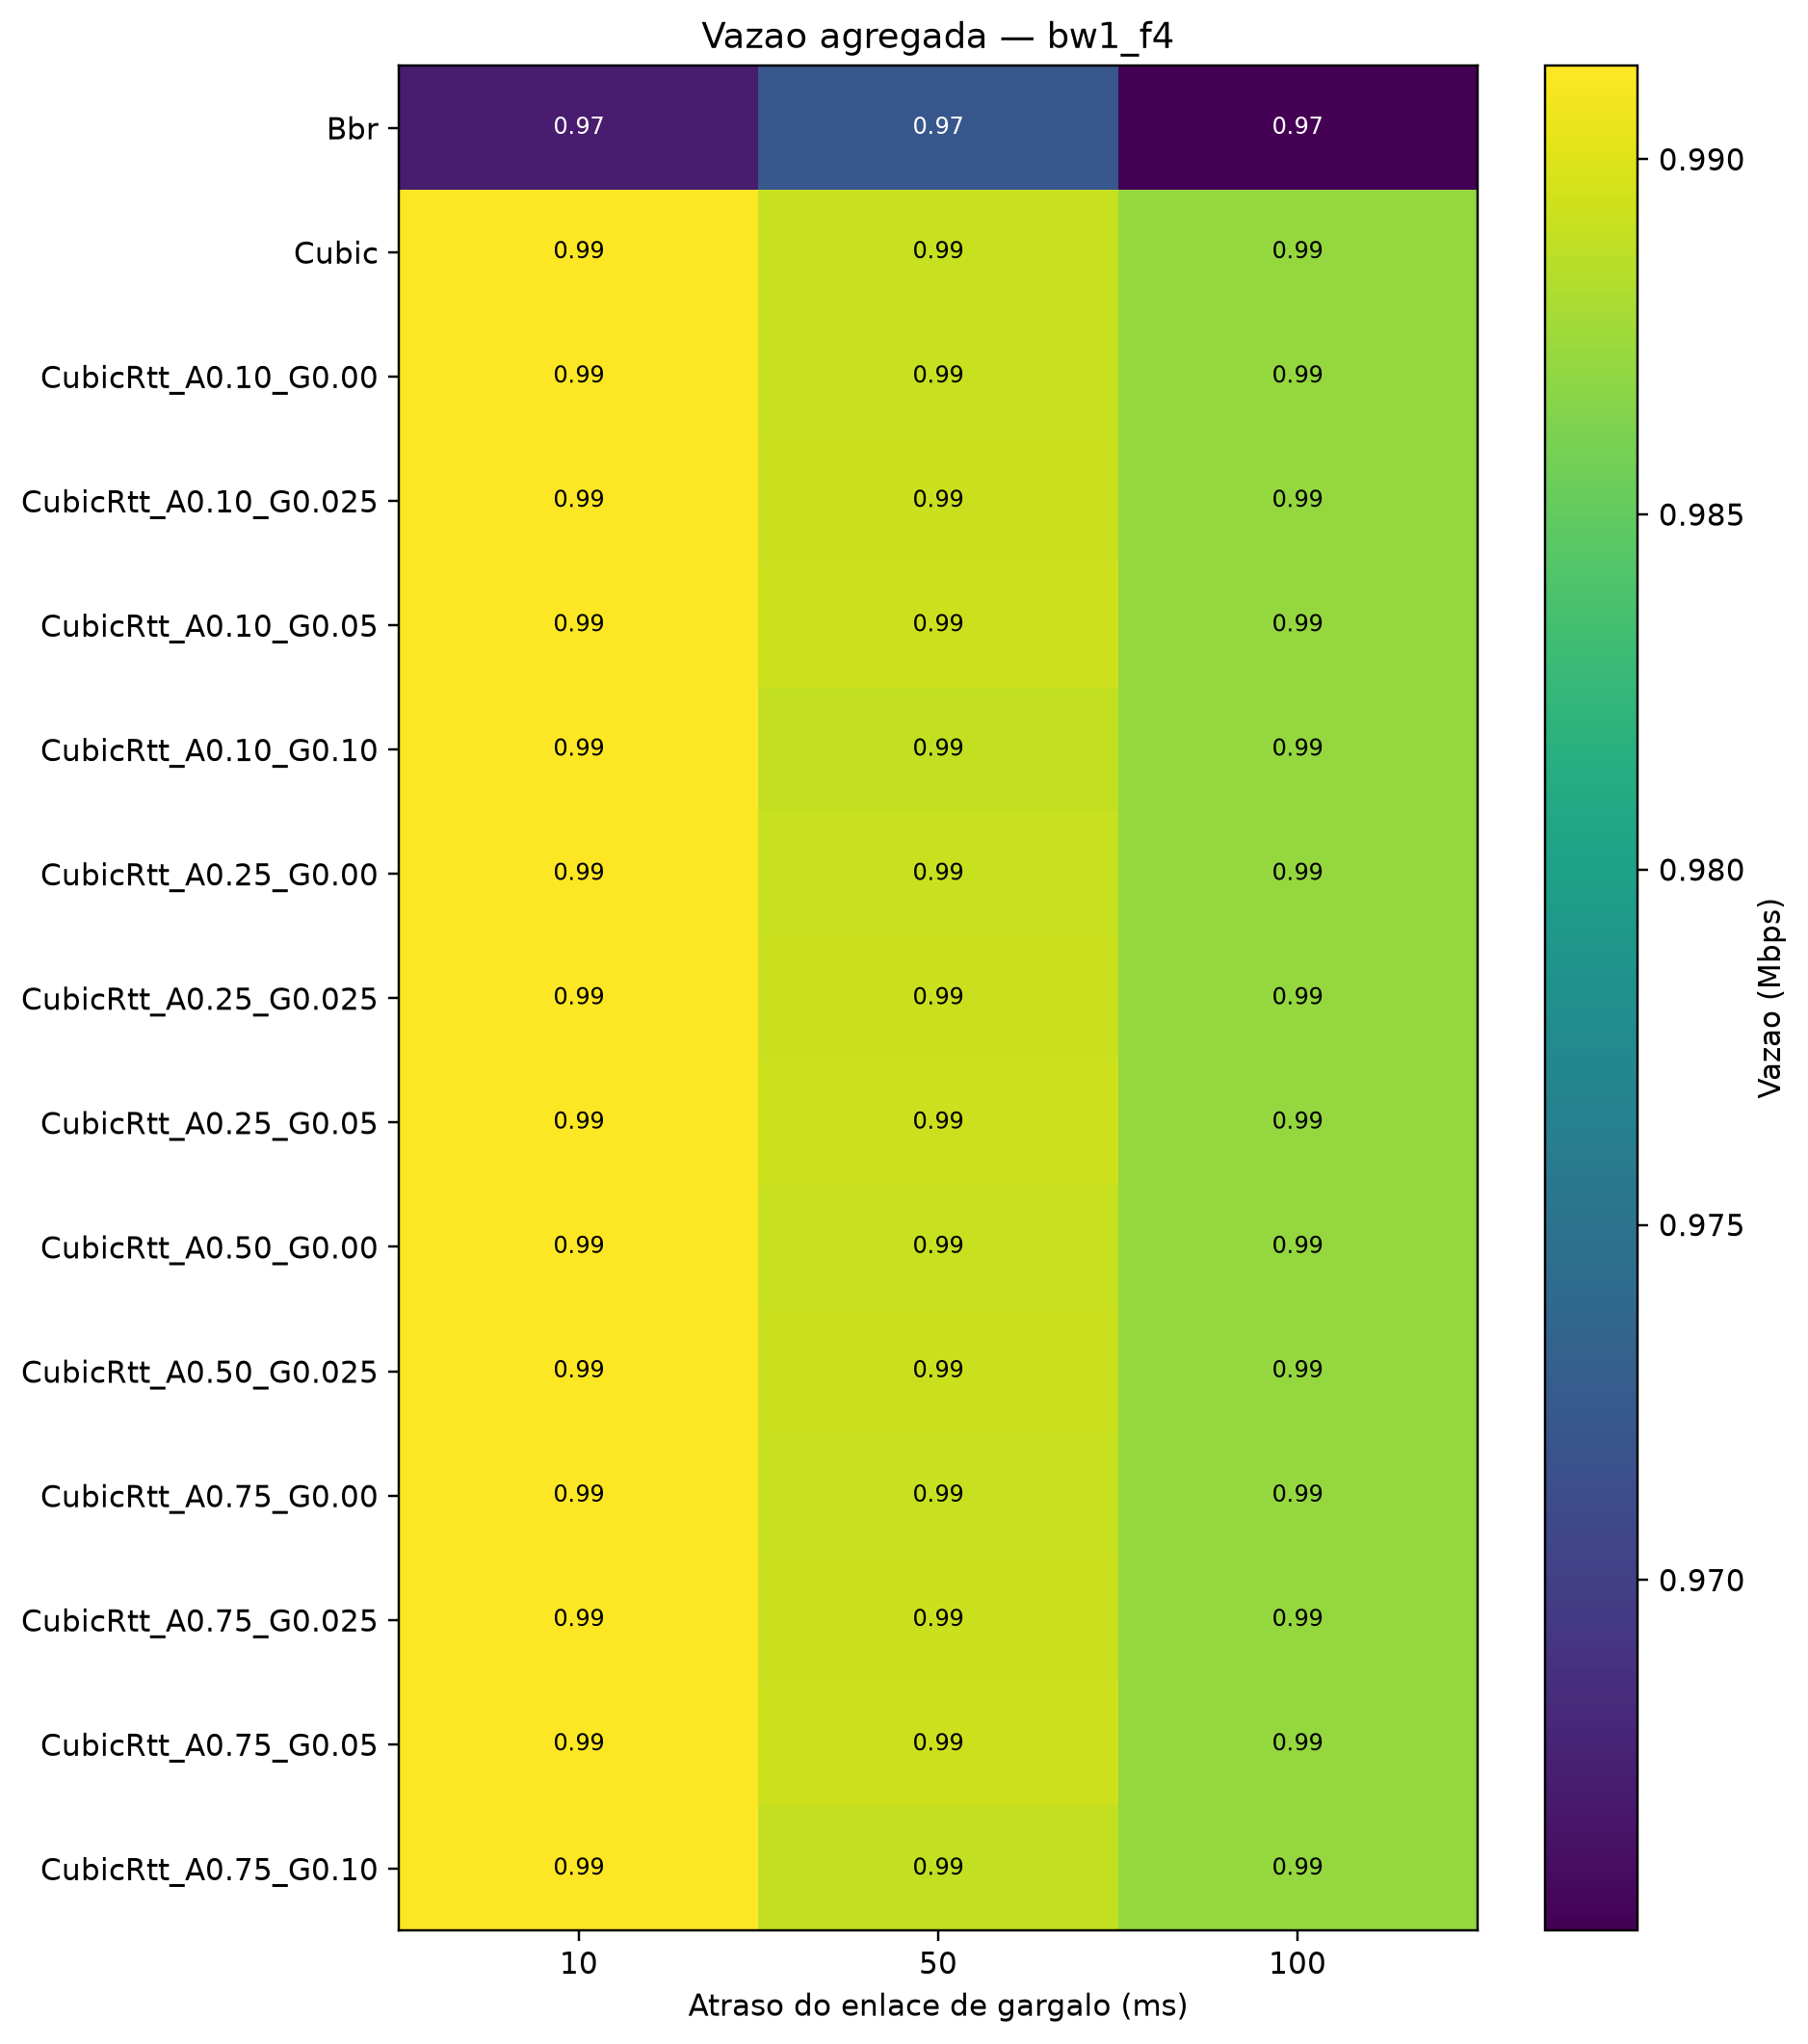
\includegraphics[width=0.88\textwidth]{bw1_f4_throughput_mbps.png}
\caption{Vazão agregada no cenário \texttt{bw1\_f4}.}
\label{fig:bw1-throughput}
\end{figure}

\begin{figure}[p]
\centering
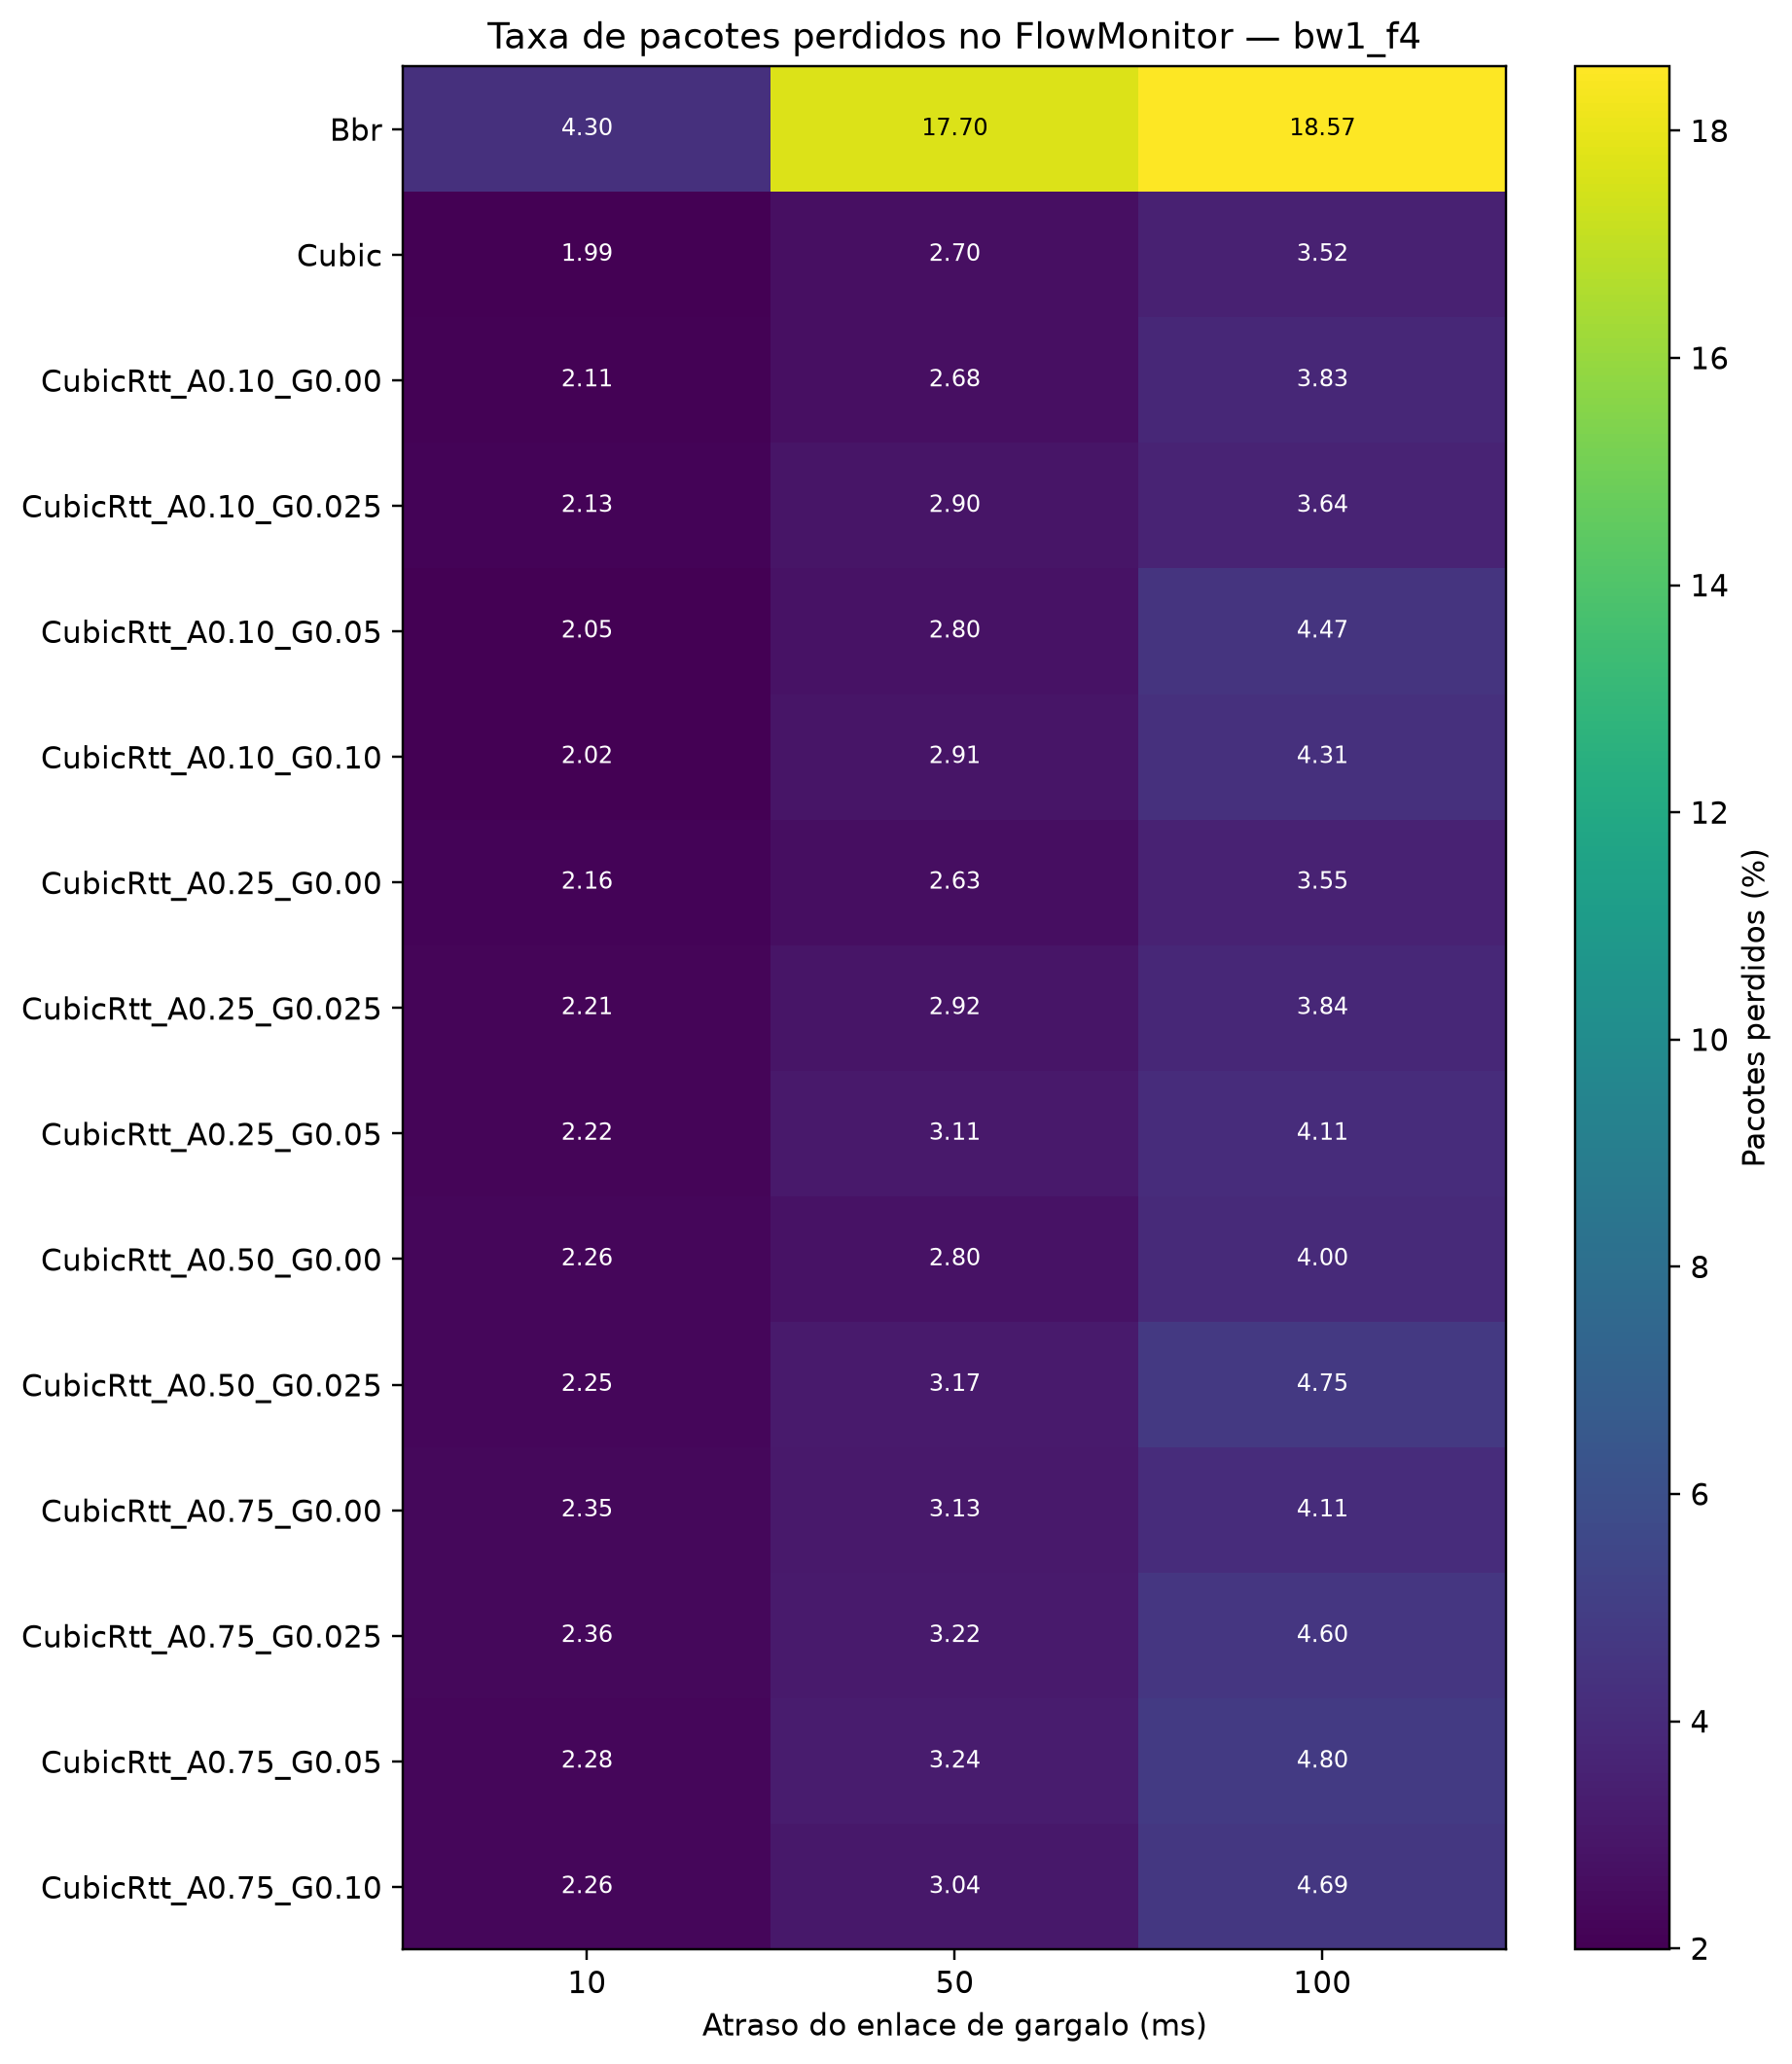
\includegraphics[width=0.88\textwidth]{bw1_f4_loss_rate_pct.png}
\caption{Taxa de perda de pacotes no cenário \texttt{bw1\_f4}.}
\label{fig:bw1-loss}
\end{figure}

\begin{figure}[p]
\centering
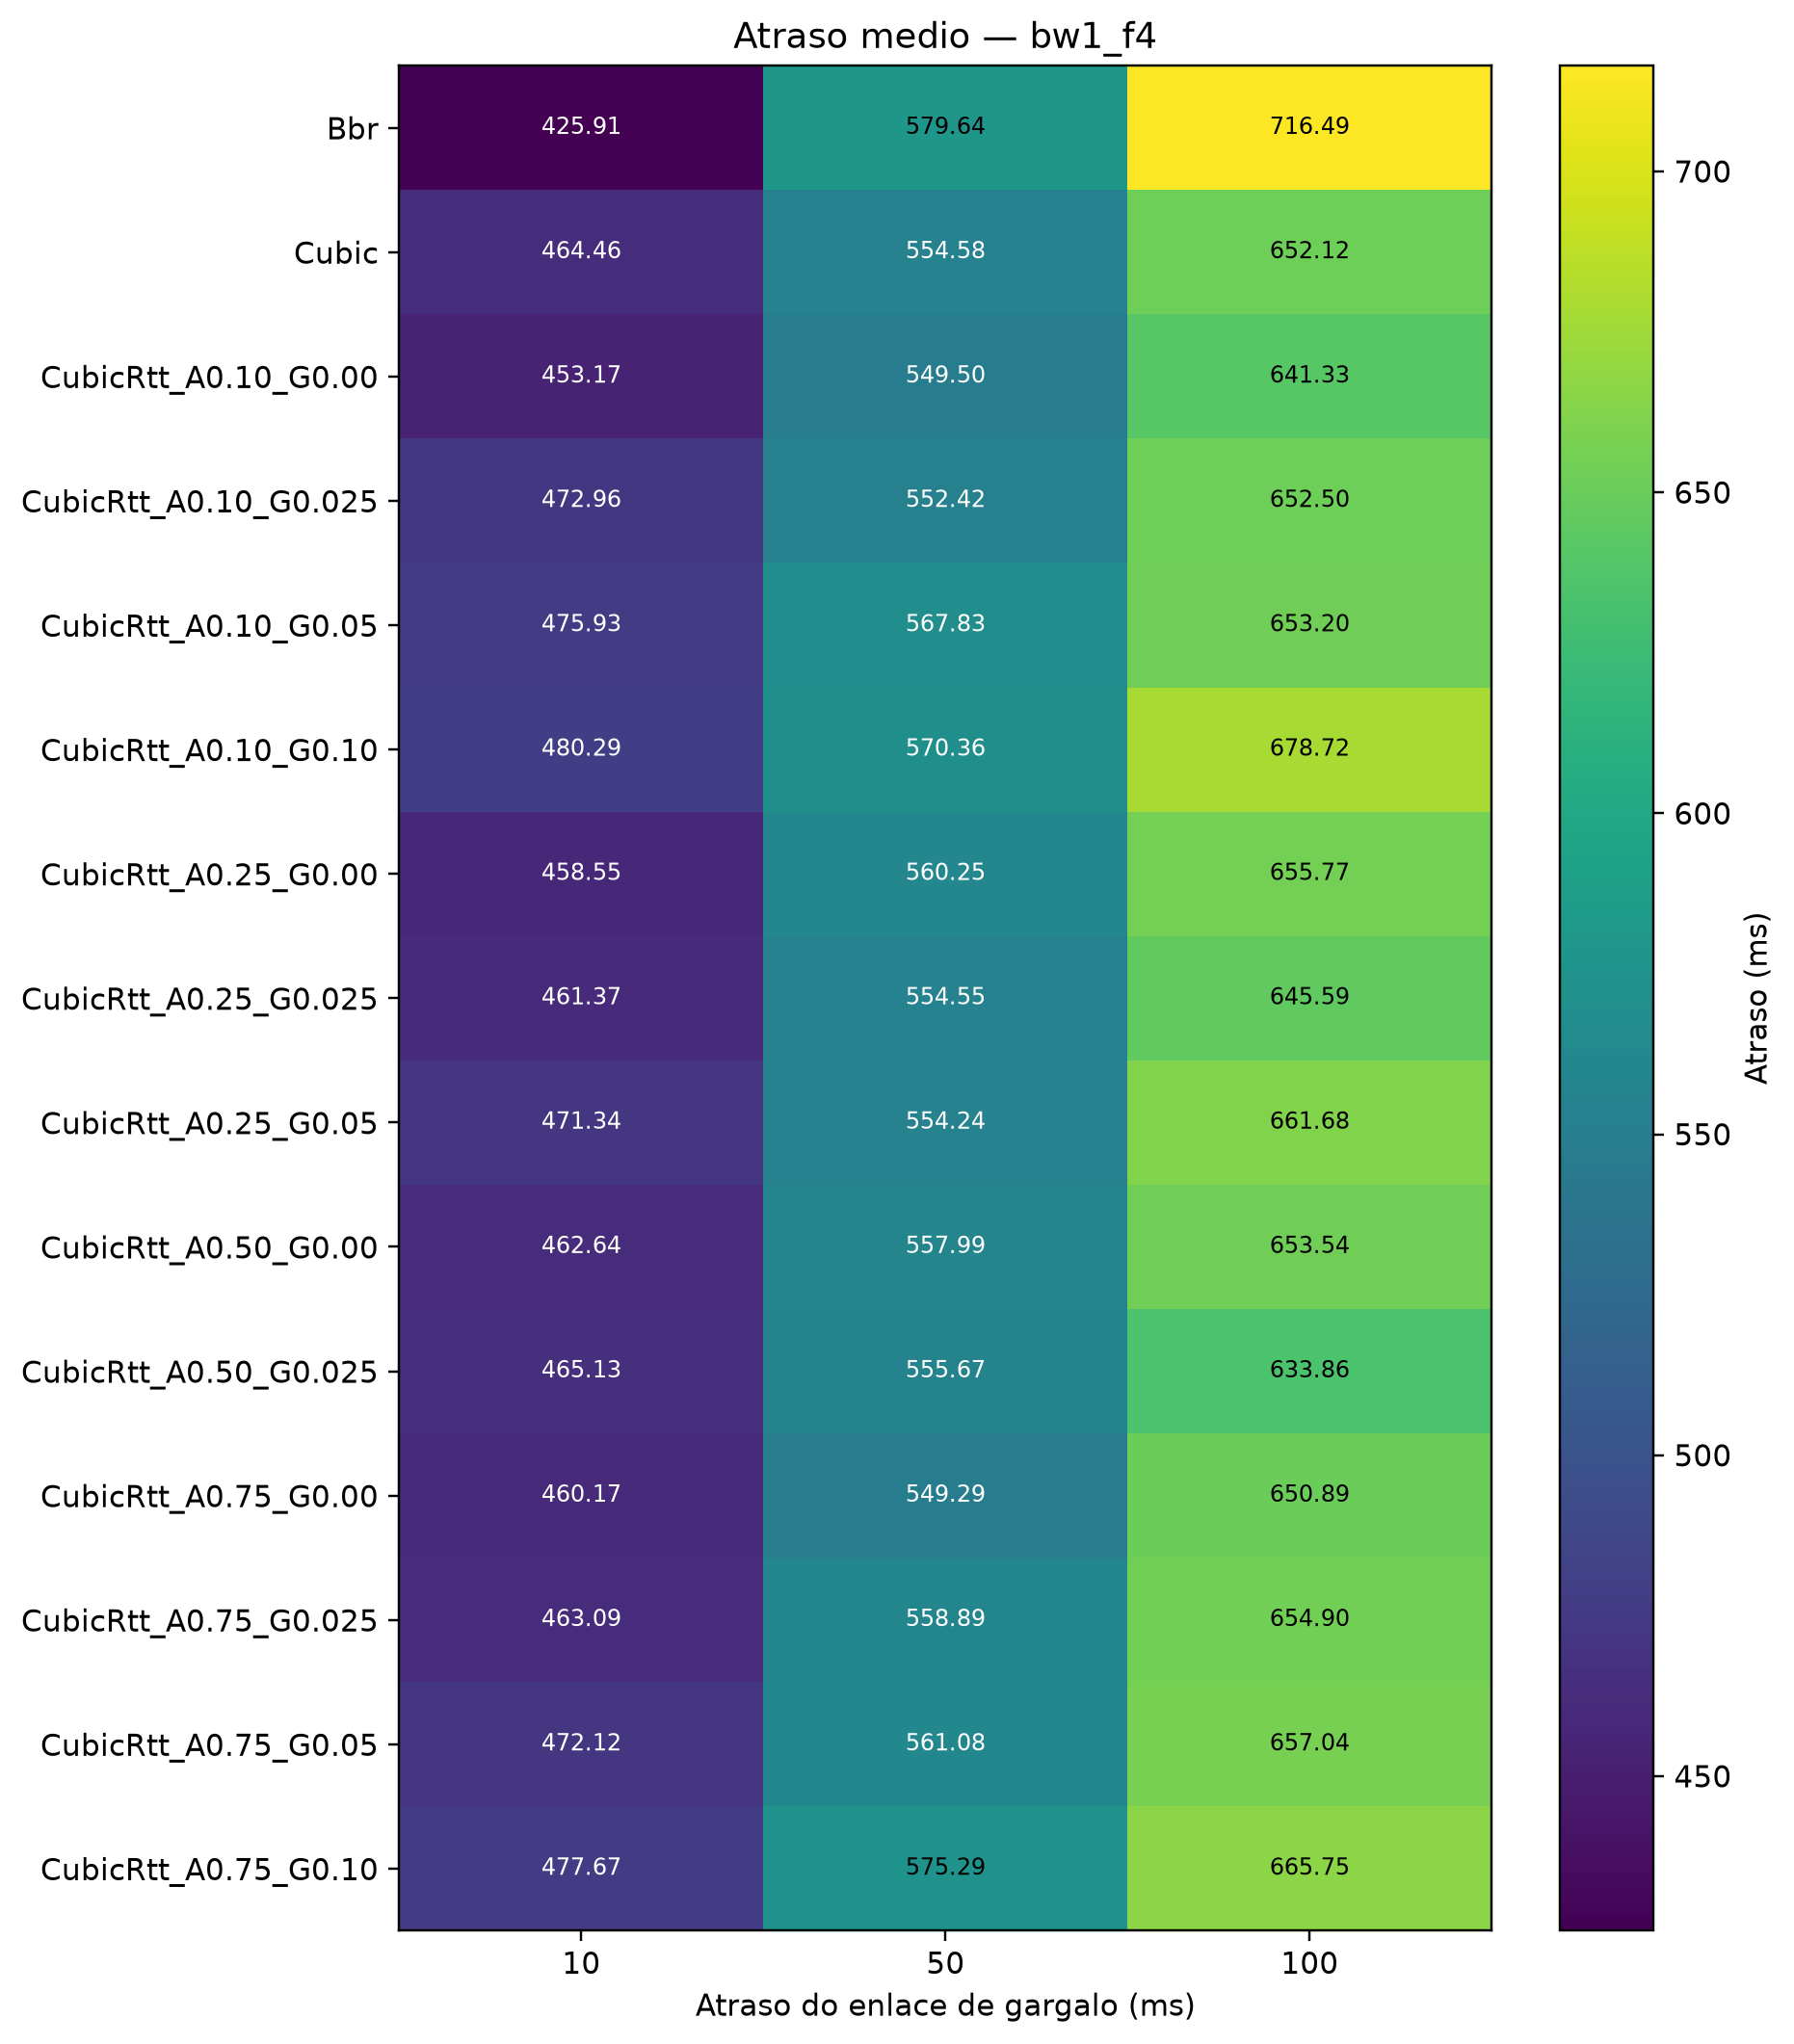
\includegraphics[width=0.88\textwidth]{bw1_f4_avg_delay_ms.png}
\caption{Atraso médio no cenário \texttt{bw1\_f4}.}
\label{fig:bw1-delay}
\end{figure}

\begin{figure}[p]
\centering
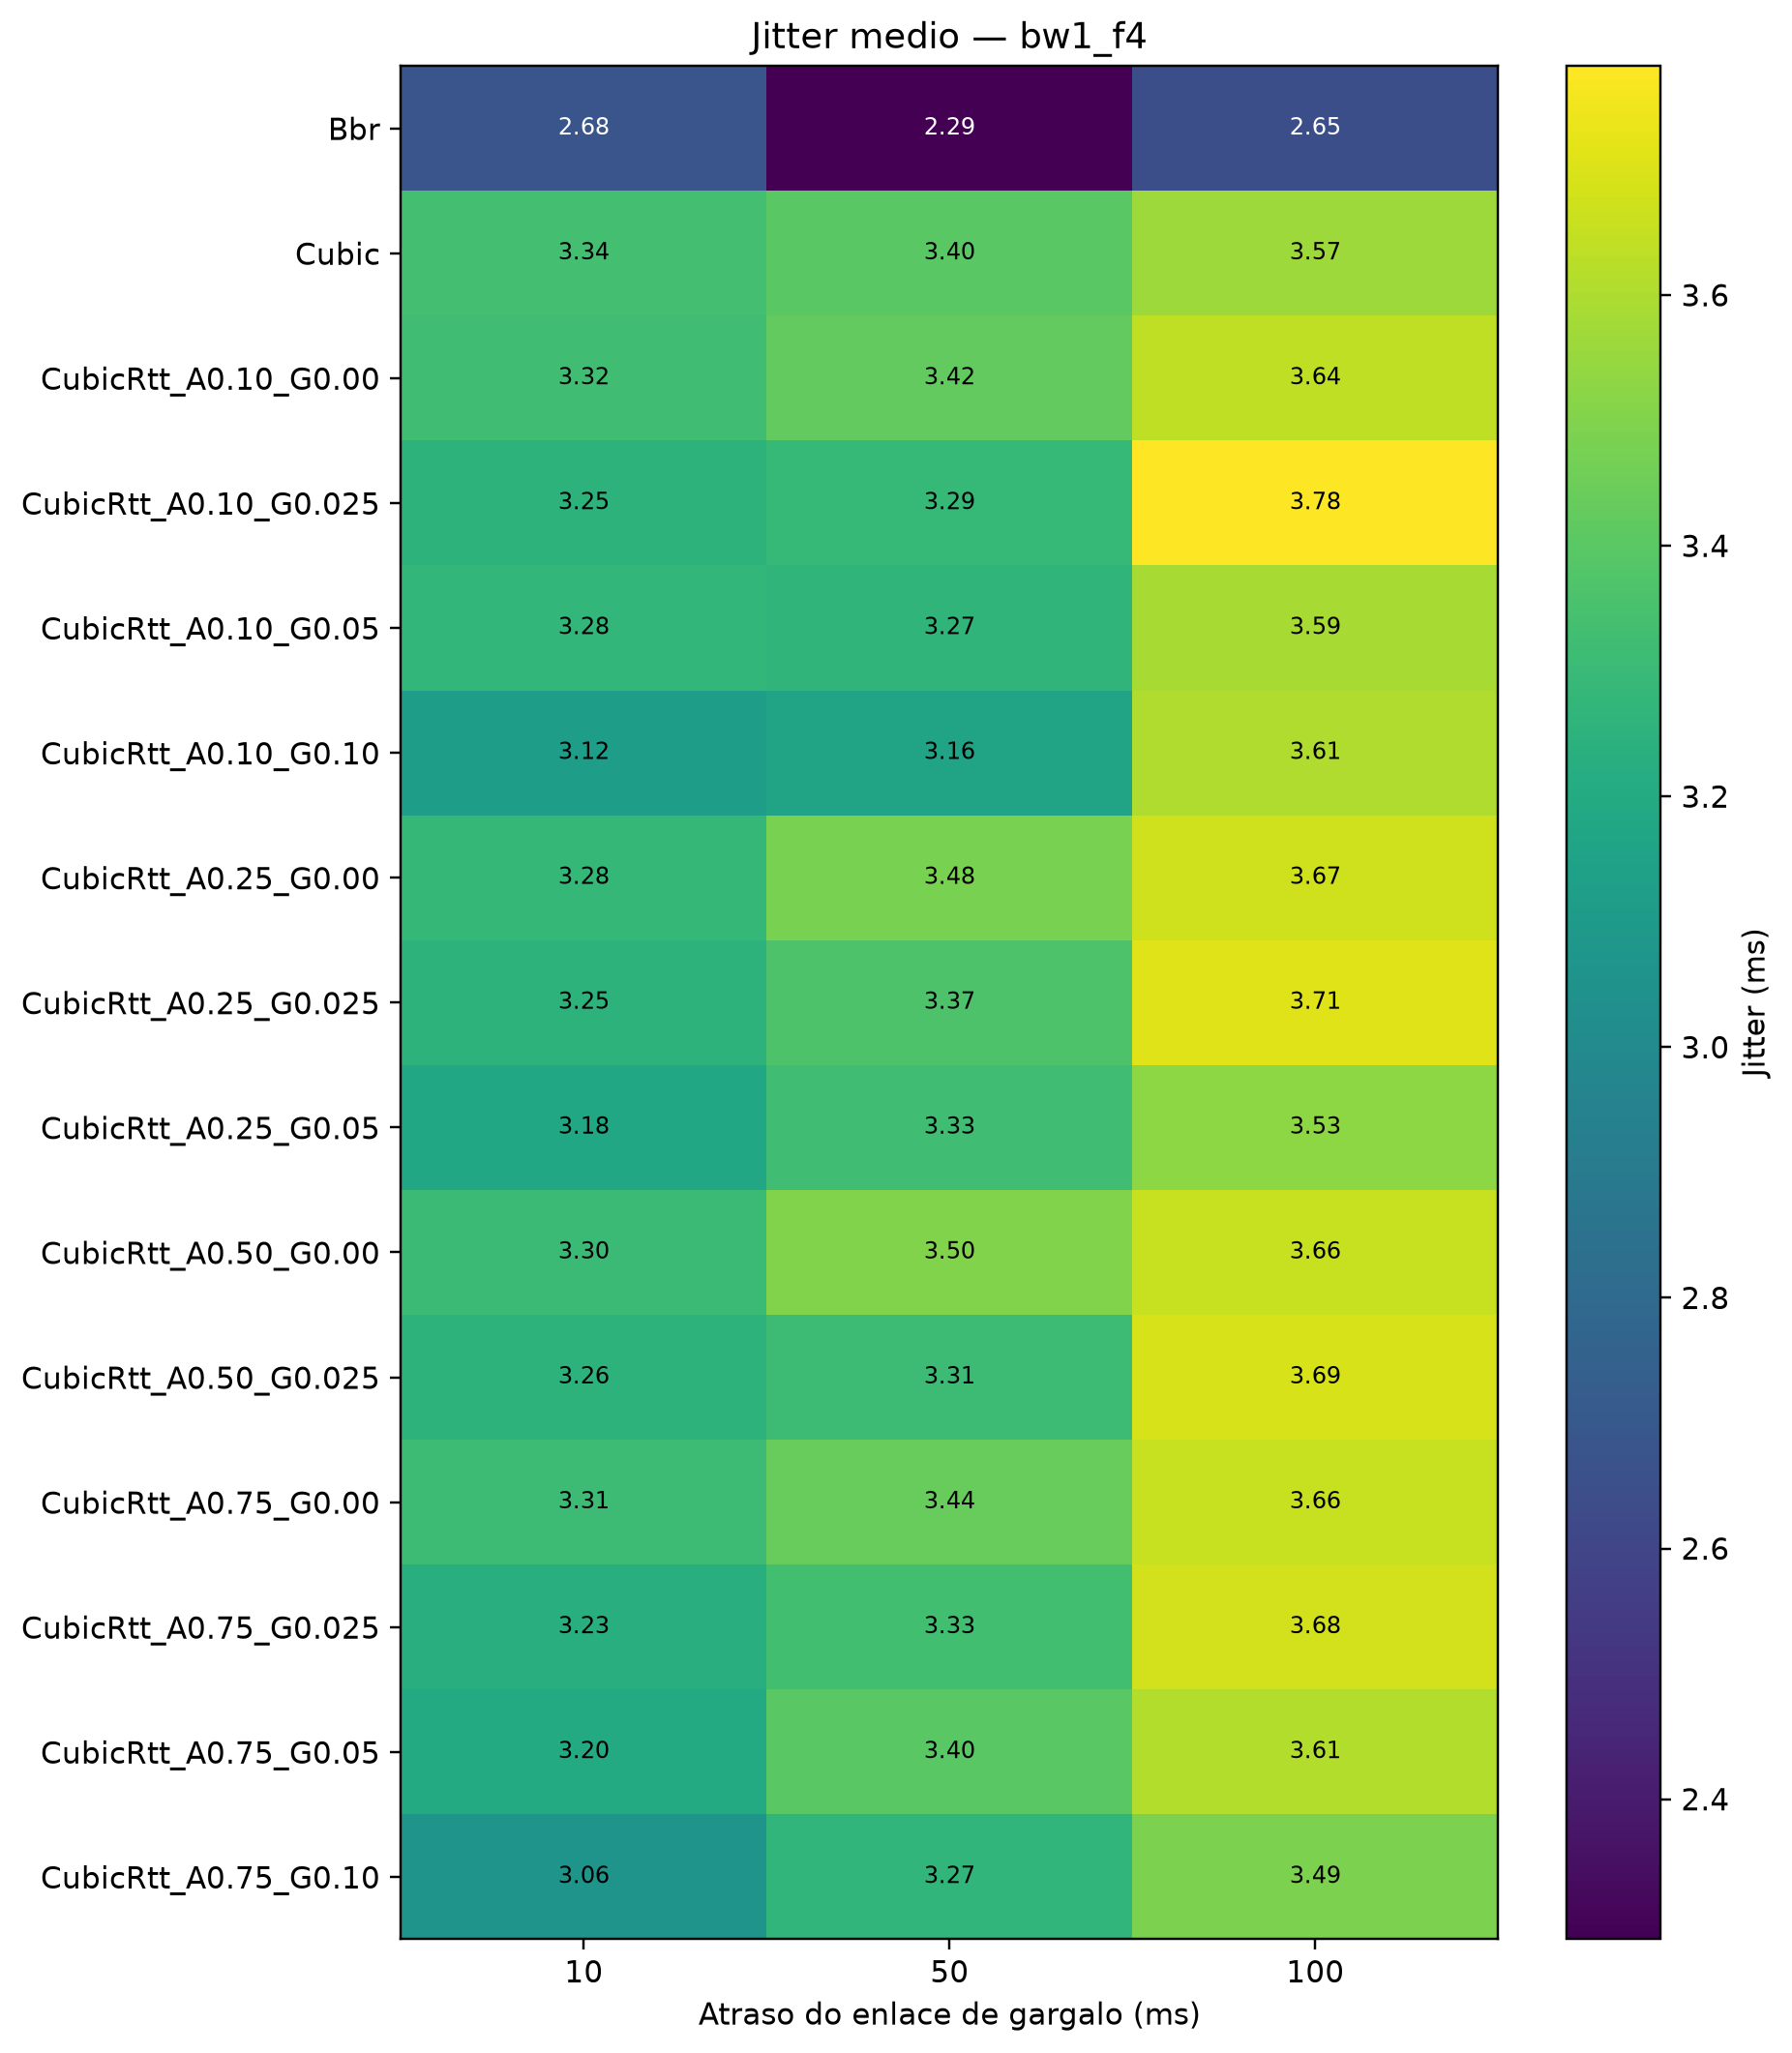
\includegraphics[width=0.88\textwidth]{bw1_f4_avg_jitter_ms.png}
\caption{Jitter médio no cenário \texttt{bw1\_f4}.}
\label{fig:bw1-jitter}
\end{figure}

\begin{figure}[p]
\centering
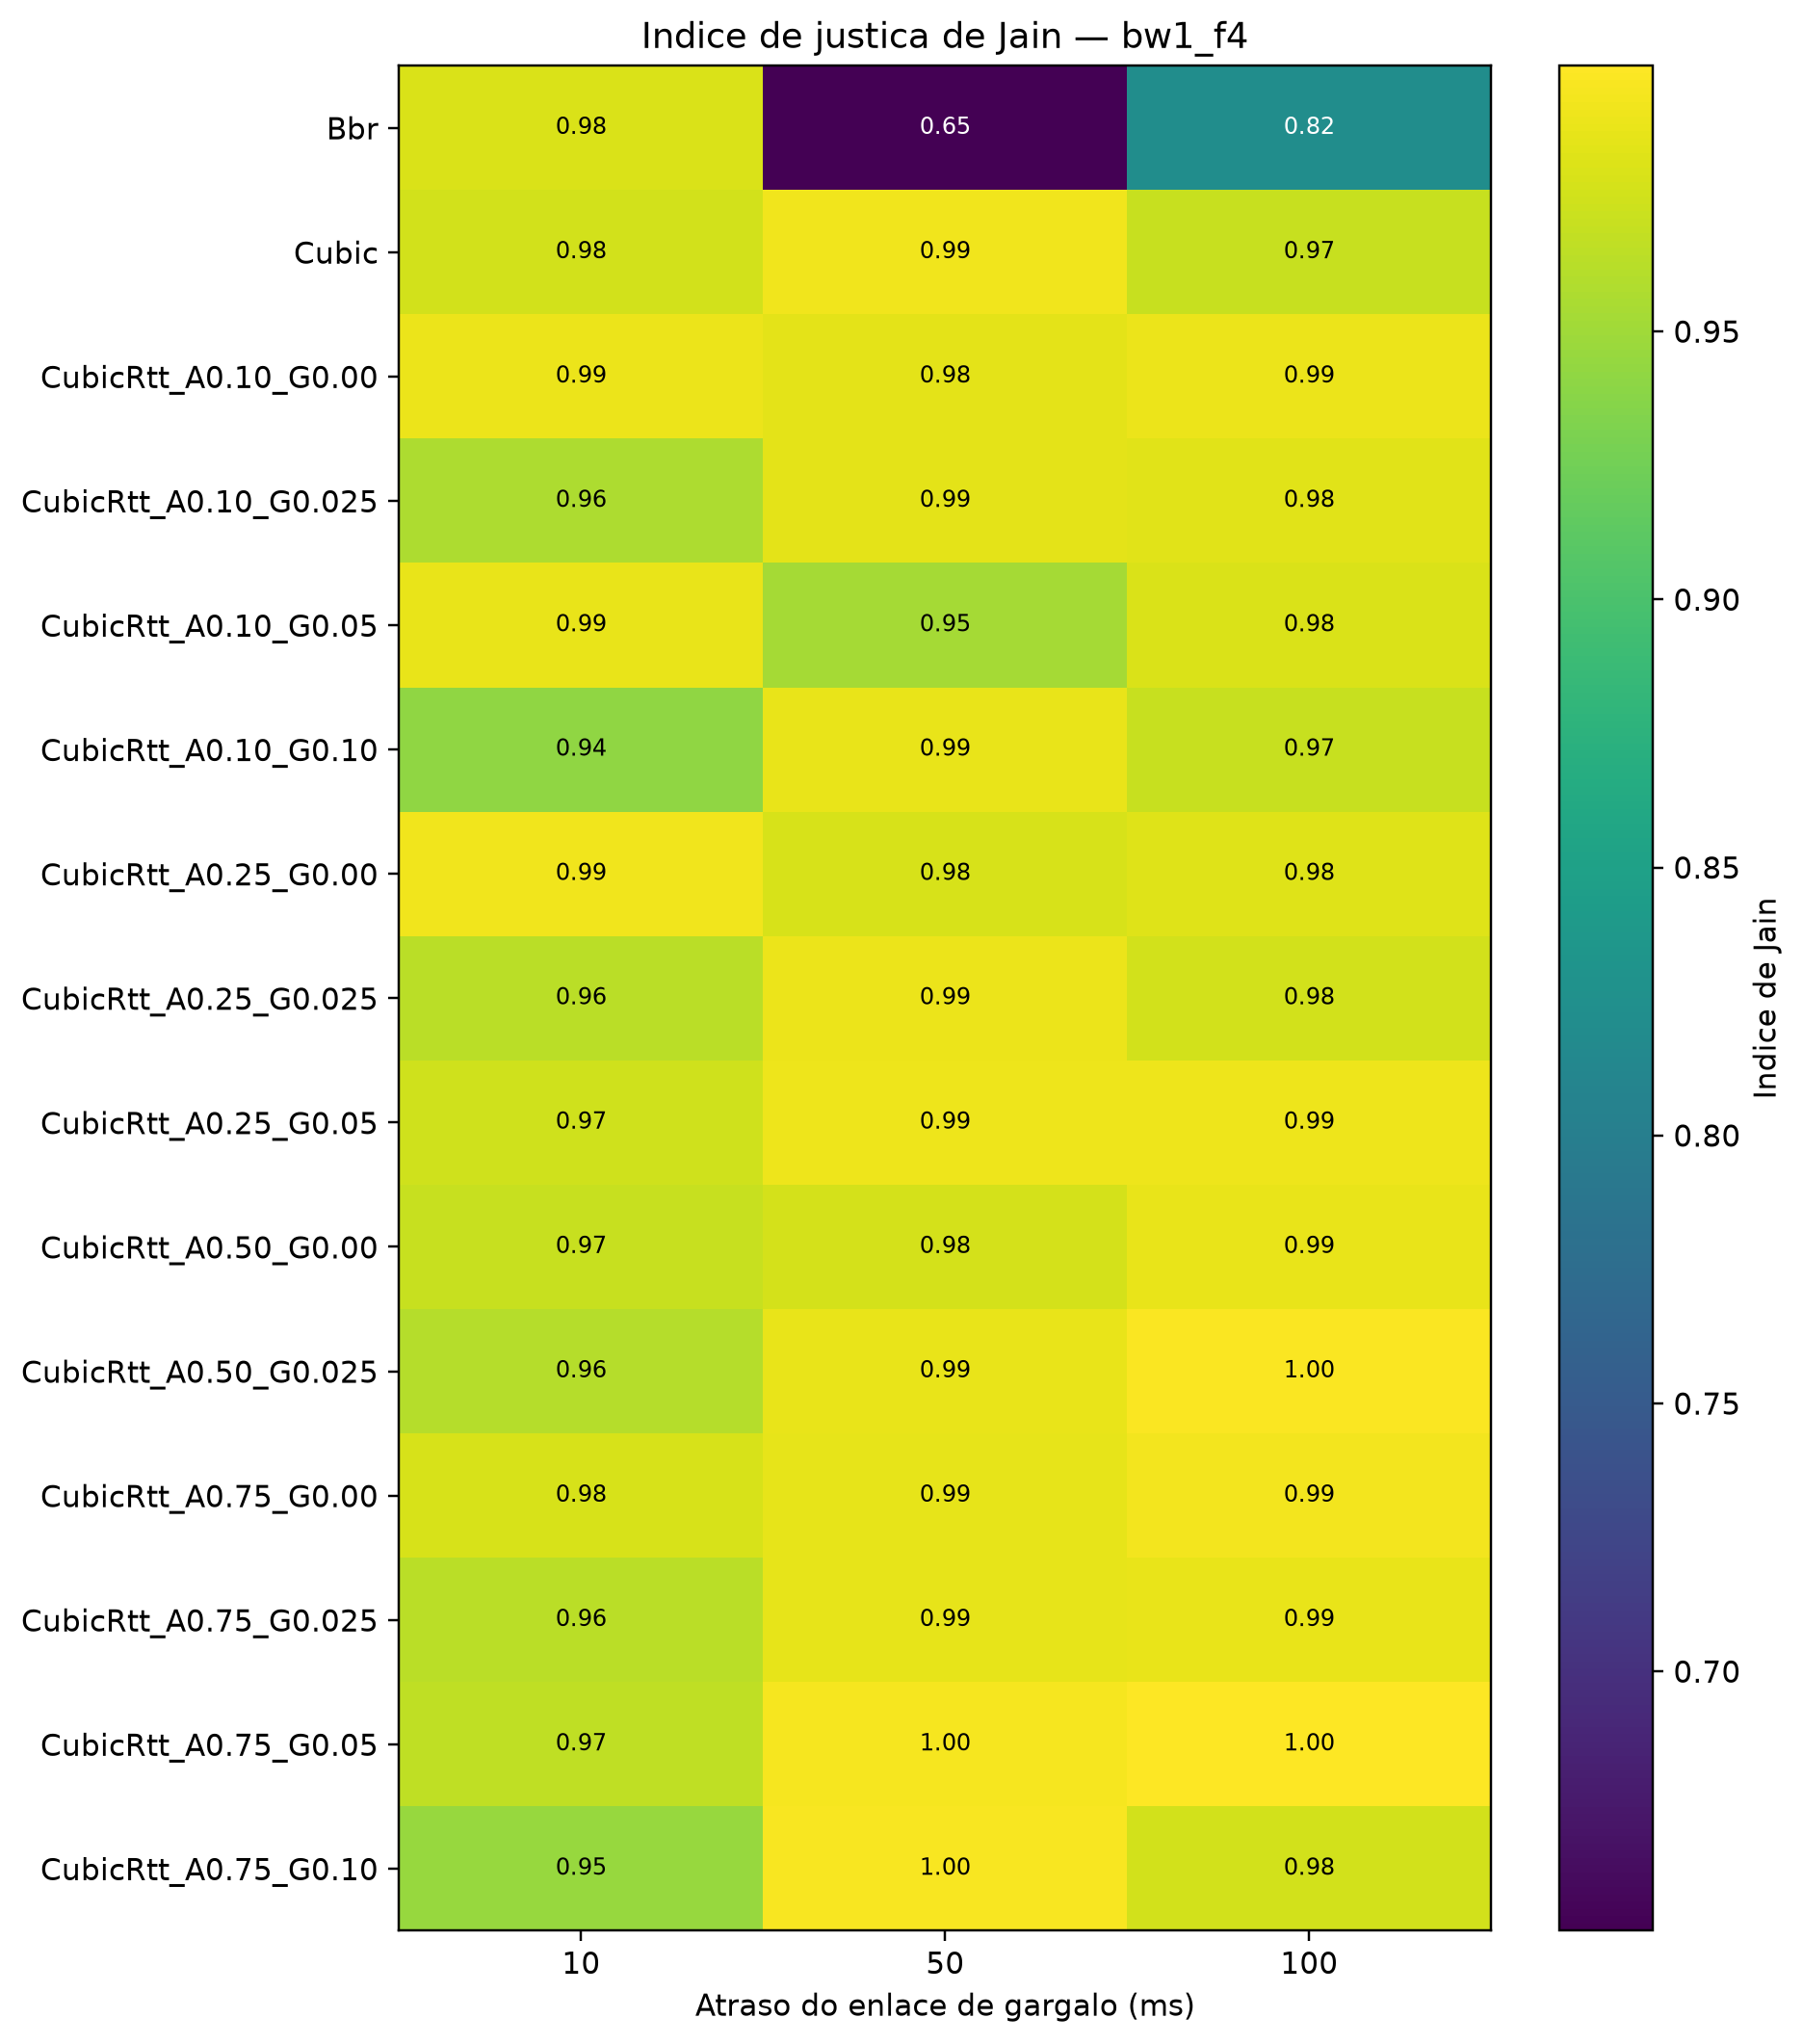
\includegraphics[width=0.88\textwidth]{bw1_f4_jain_fairness.png}
\caption{Índice de Justiça de Jain no cenário \texttt{bw1\_f4}.}
\label{fig:bw1-jain}
\end{figure}

\section{Cenário bw2\_f8}

\begin{figure}[p]
\centering
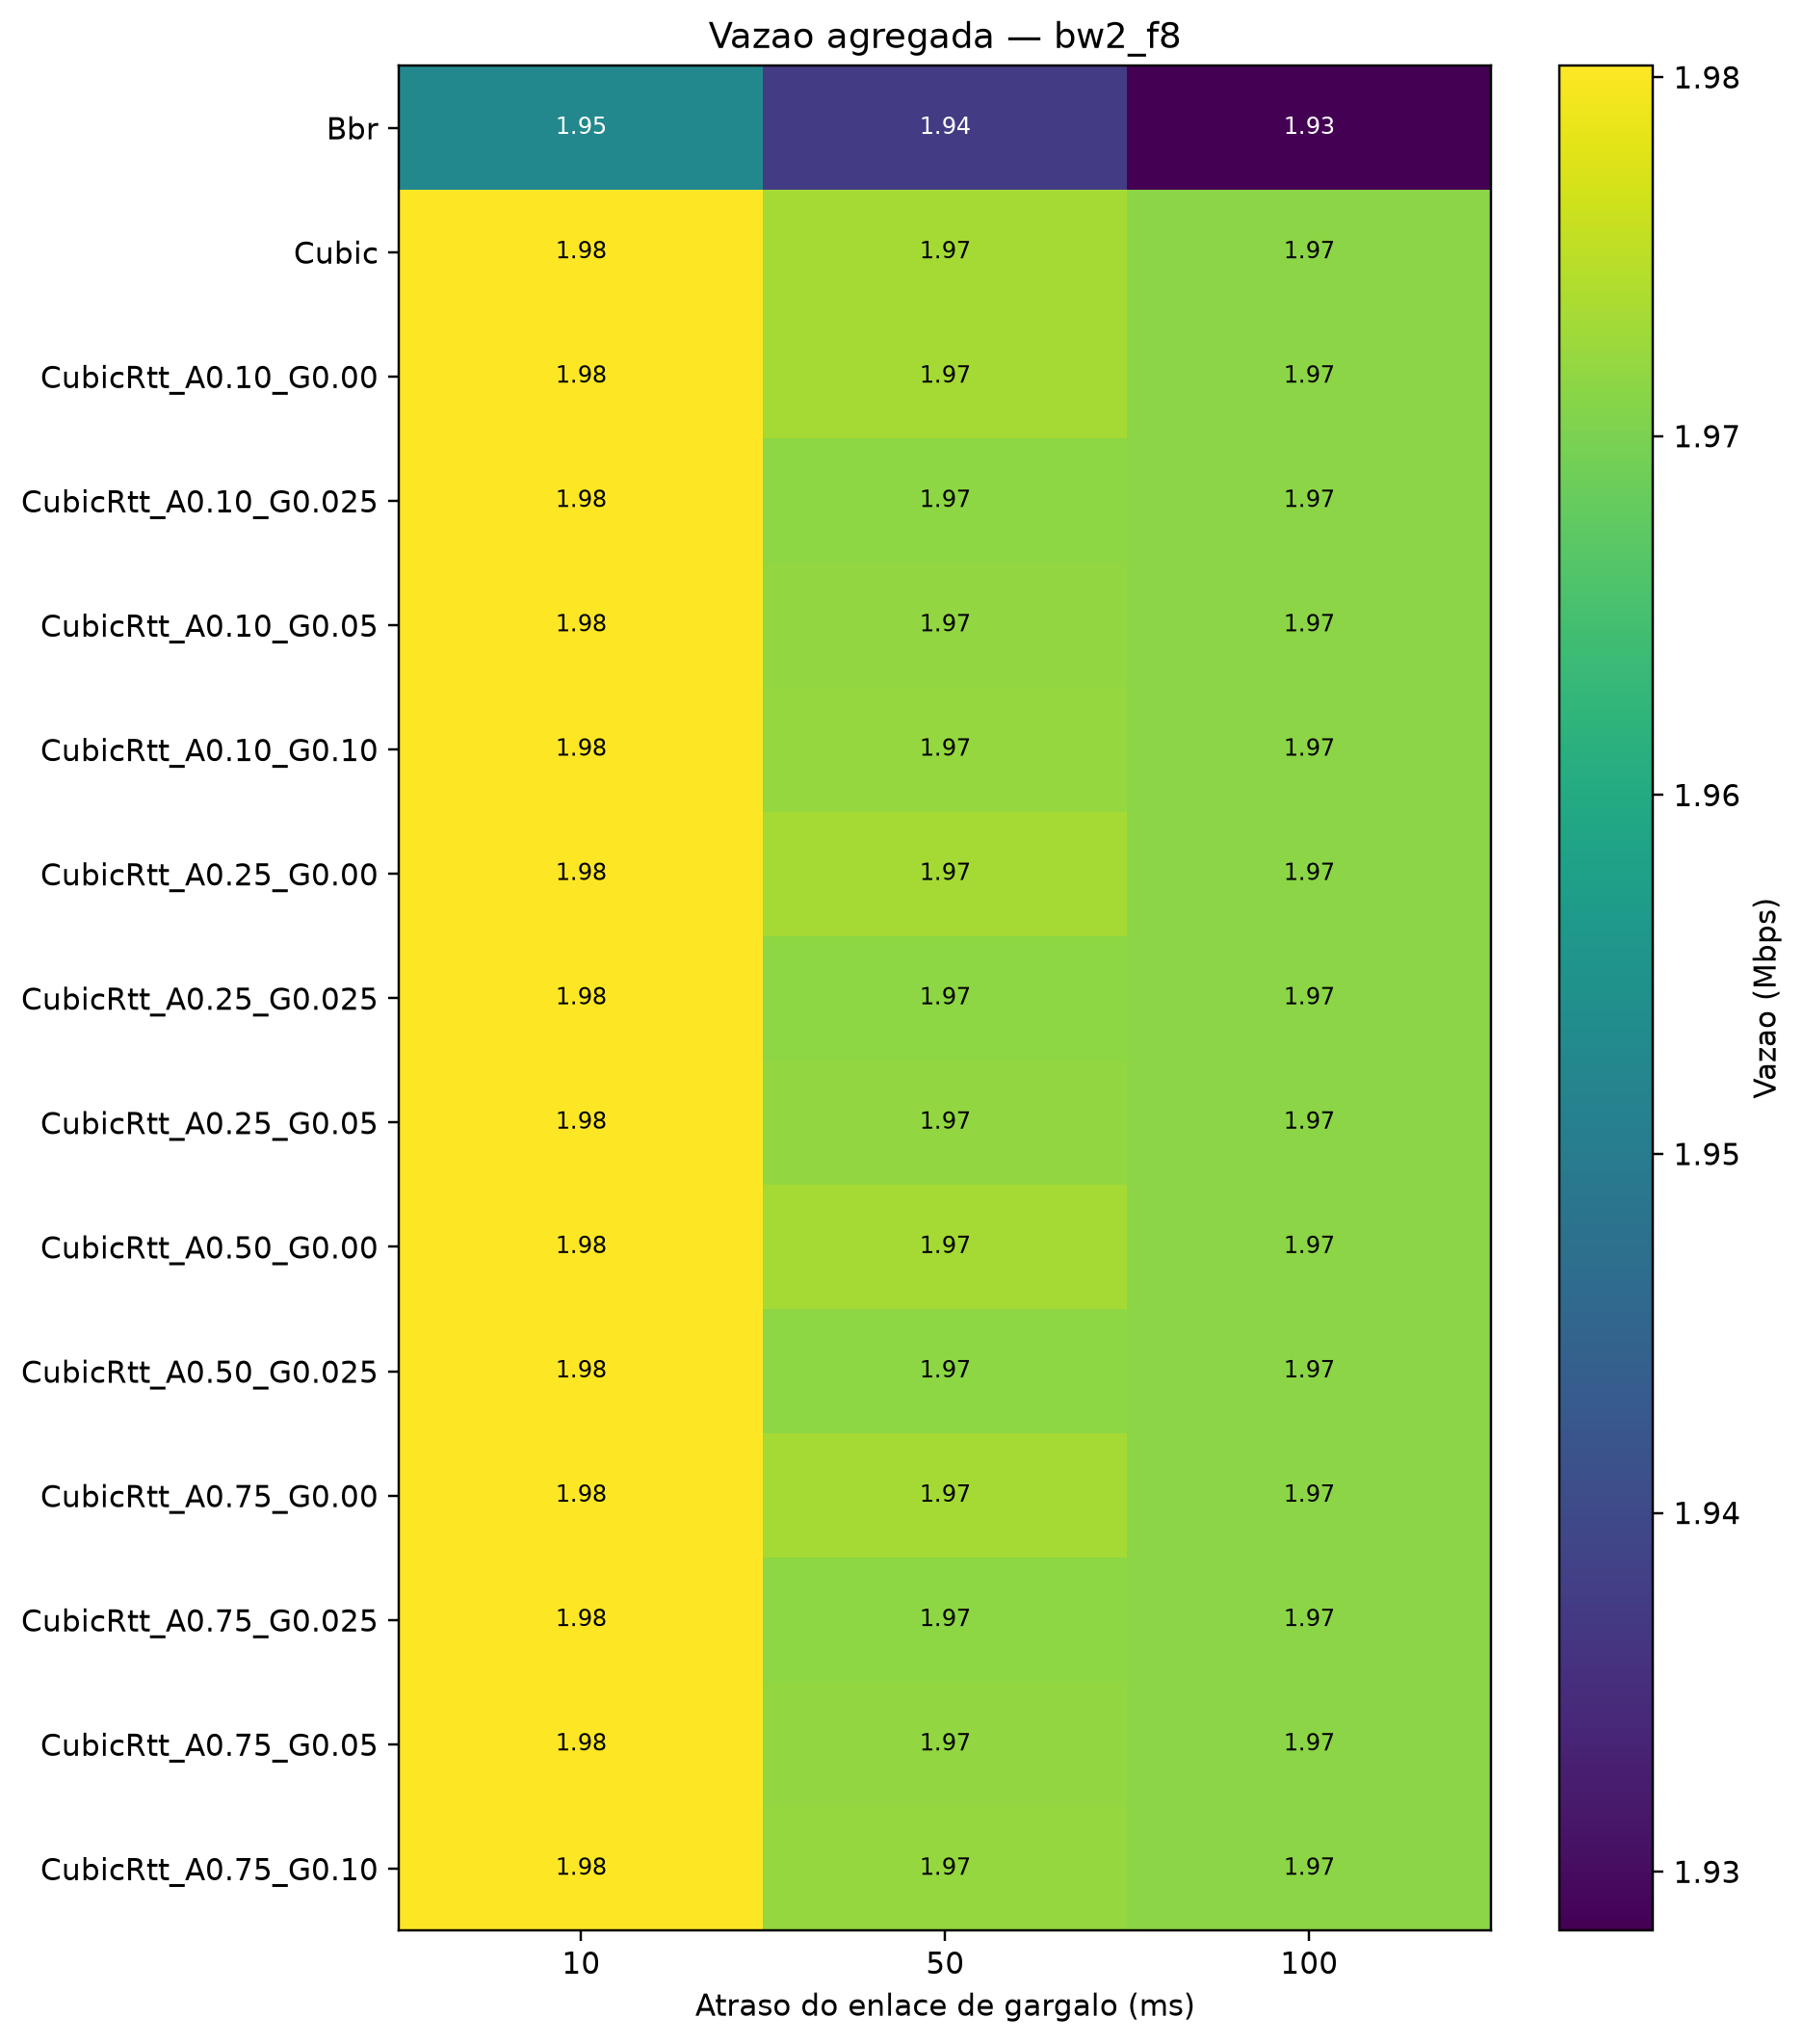
\includegraphics[width=0.88\textwidth]{bw2_f8_throughput_mbps.png}
\caption{Vazão agregada no cenário \texttt{bw2\_f8}.}
\label{fig:bw2-throughput}
\end{figure}

\begin{figure}[p]
\centering
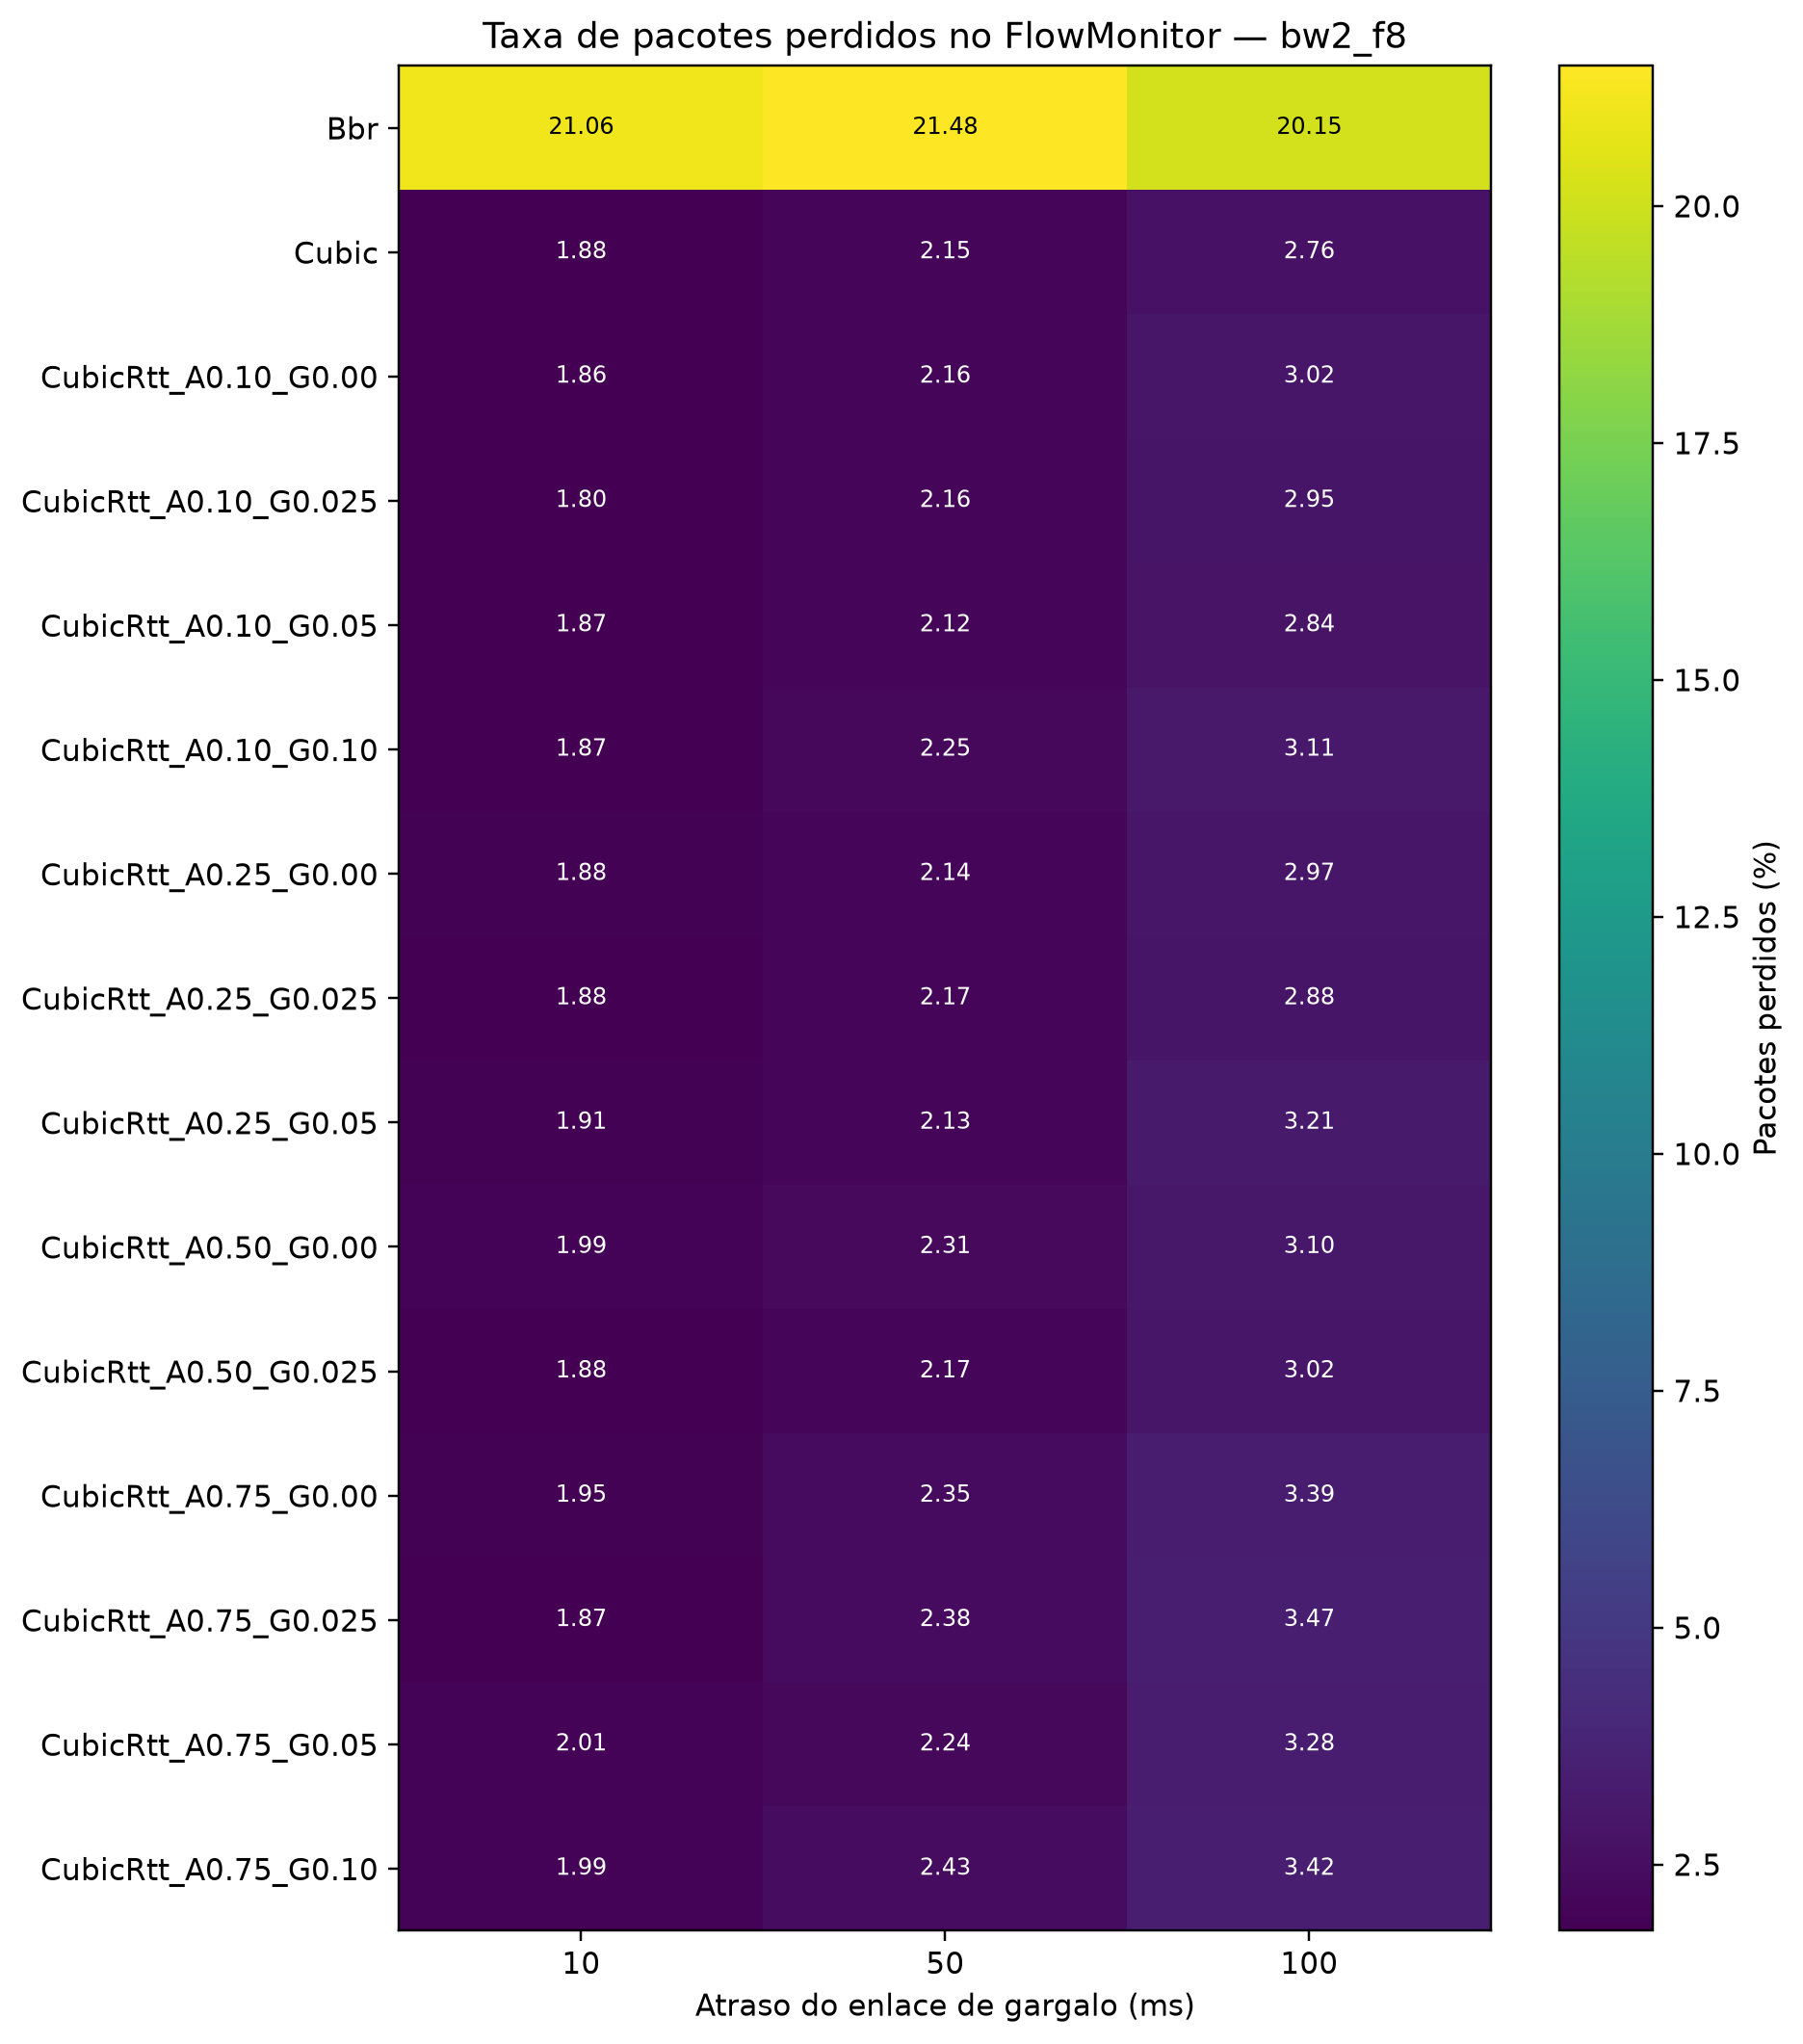
\includegraphics[width=0.88\textwidth]{bw2_f8_loss_rate_pct.png}
\caption{Taxa de perda de pacotes no cenário \texttt{bw2\_f8}.}
\label{fig:bw2-loss}
\end{figure}

\begin{figure}[p]
\centering
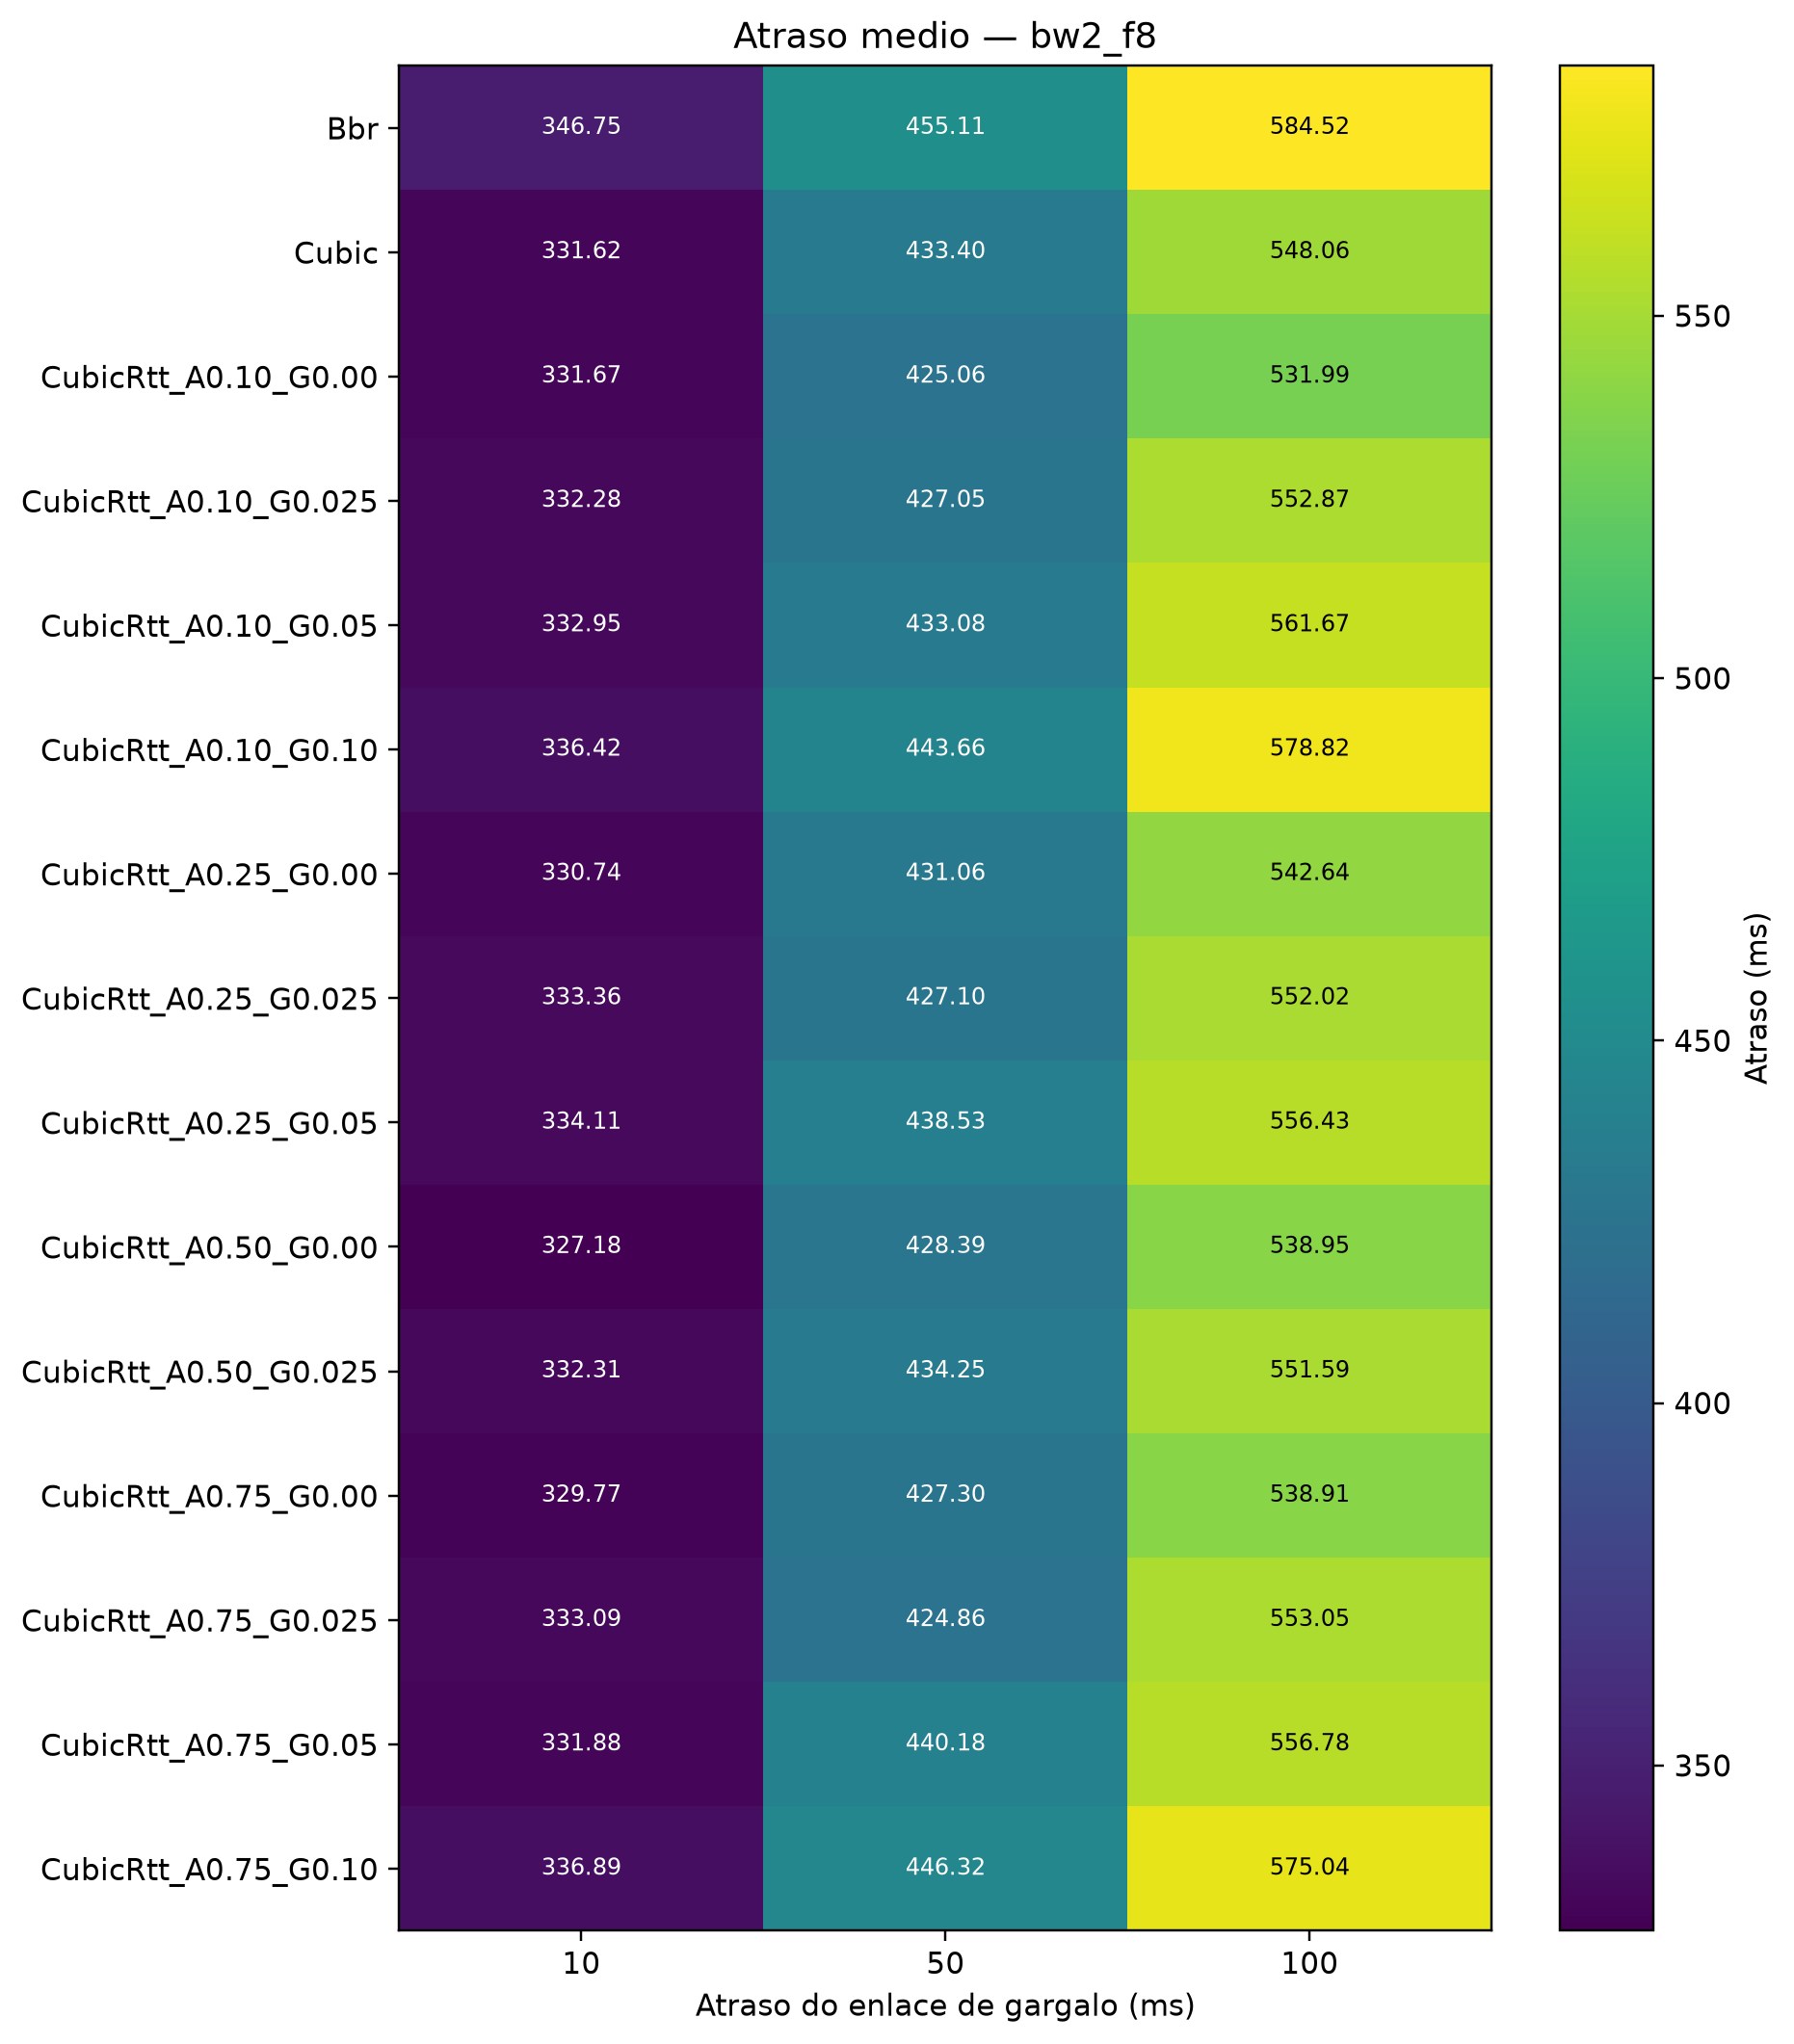
\includegraphics[width=0.88\textwidth]{bw2_f8_avg_delay_ms.png}
\caption{Atraso médio no cenário \texttt{bw2\_f8}.}
\label{fig:bw2-delay}
\end{figure}

\begin{figure}[p]
\centering
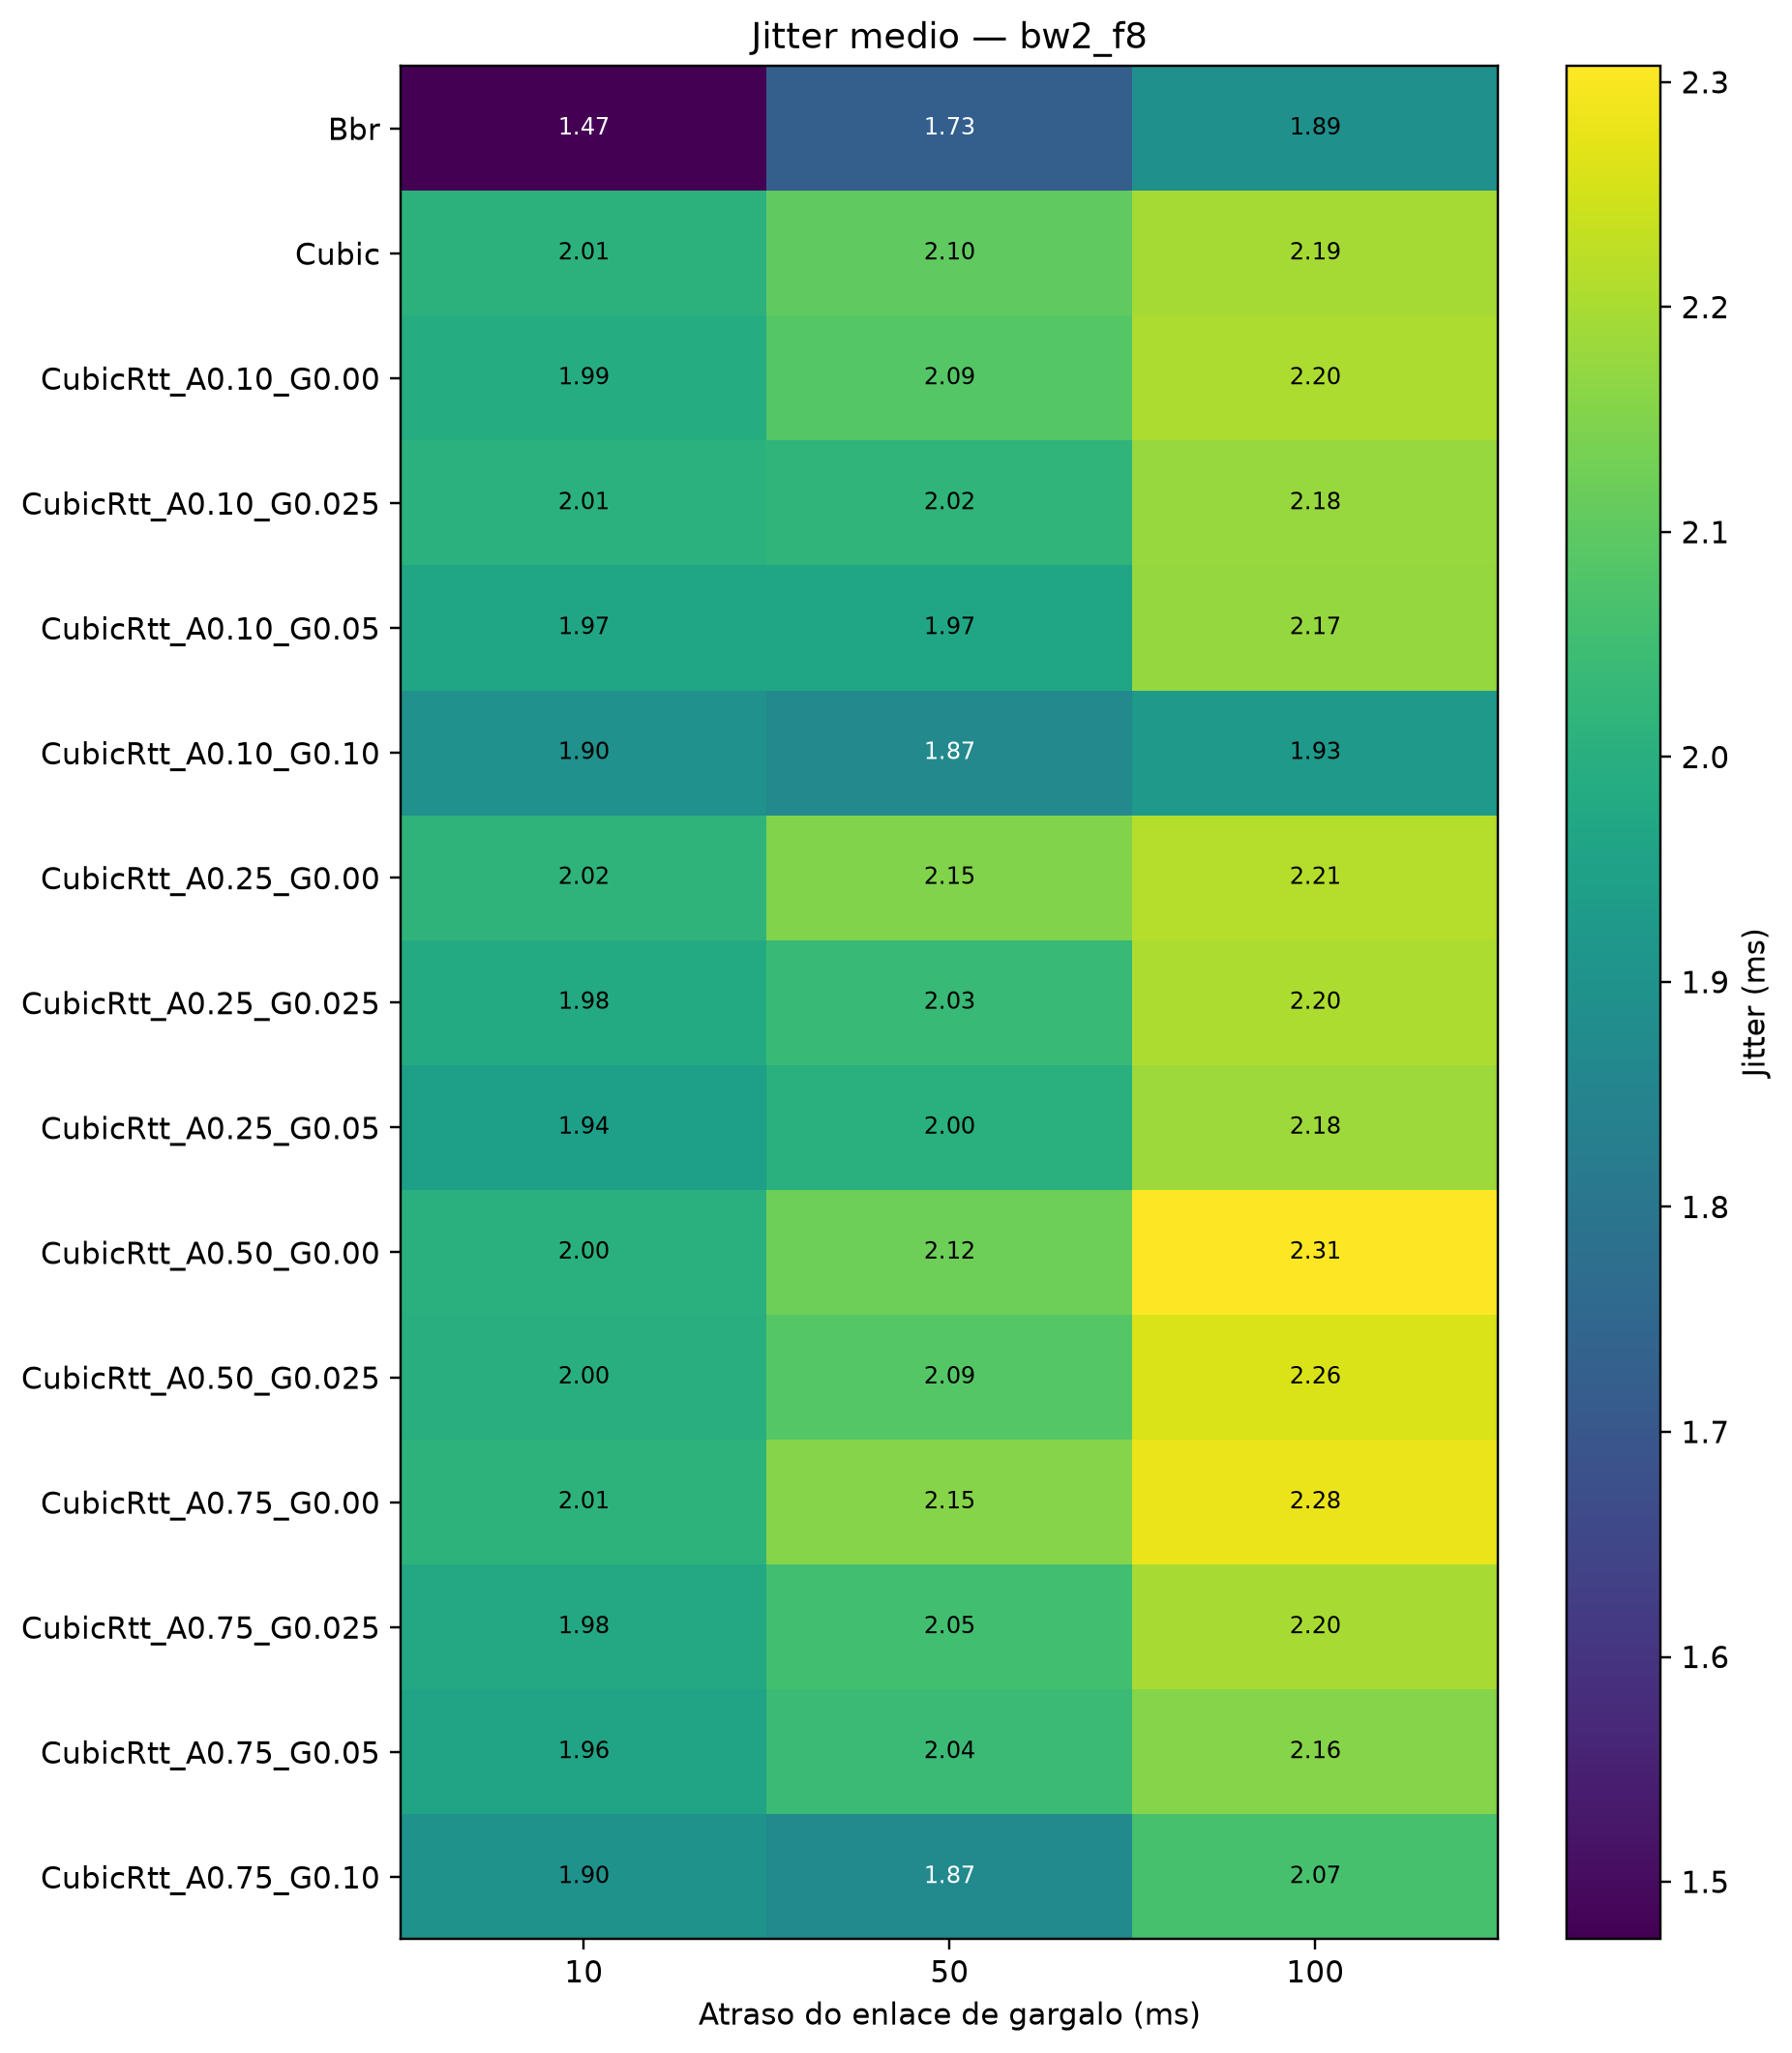
\includegraphics[width=0.88\textwidth]{bw2_f8_avg_jitter_ms.png}
\caption{Jitter médio no cenário \texttt{bw2\_f8}.}
\label{fig:bw2-jitter}
\end{figure}

\begin{figure}[p]
\centering
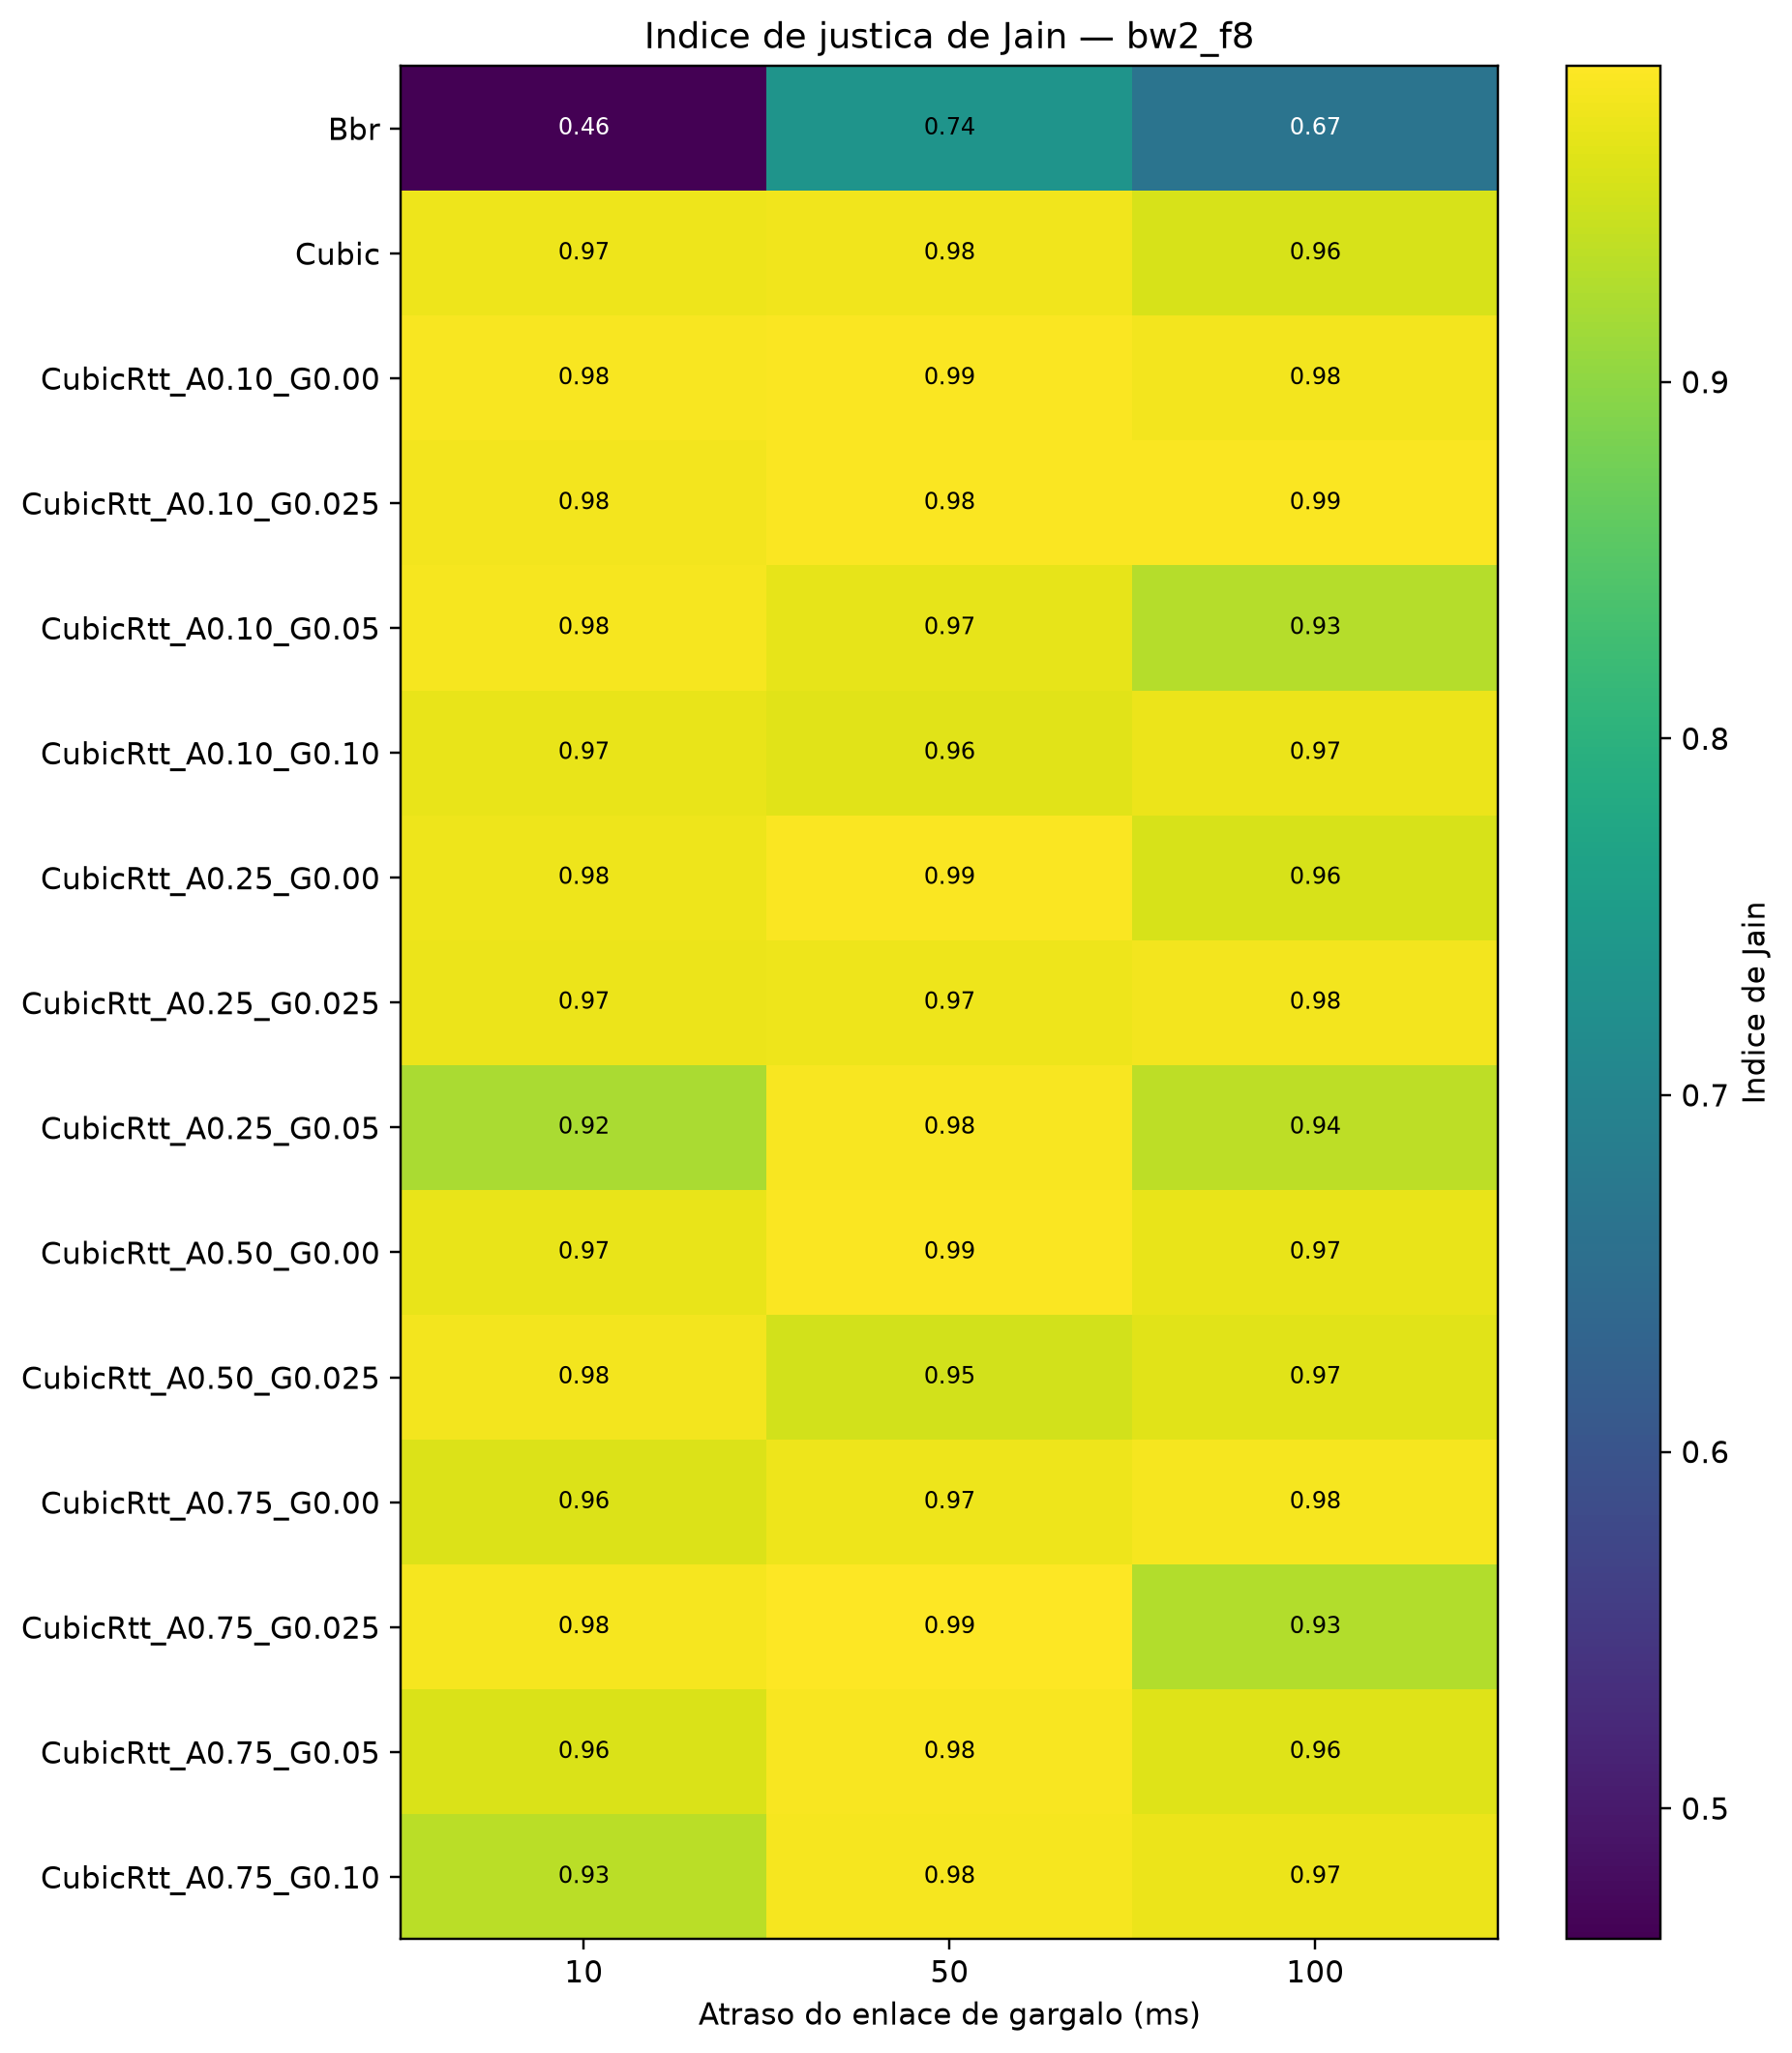
\includegraphics[width=0.88\textwidth]{bw2_f8_jain_fairness.png}
\caption{Índice de Justiça de Jain no cenário \texttt{bw2\_f8}.}
\label{fig:bw2-jain}
\end{figure}

\chapter{Rastros Temporais da Campanha de Coexistência}
\label{ap:traces}

Os gráficos apresentam exemplos da evolução temporal da janela de congestionamento e do RTT dos oito fluxos simultâneos. Eles complementam a análise agregada do Capítulo~\ref{cap:resultados}, permitindo observar a dinâmica das conexões durante as execuções.

\section{Atraso de gargalo de 10 ms}

\begin{figure}[p]
\centering
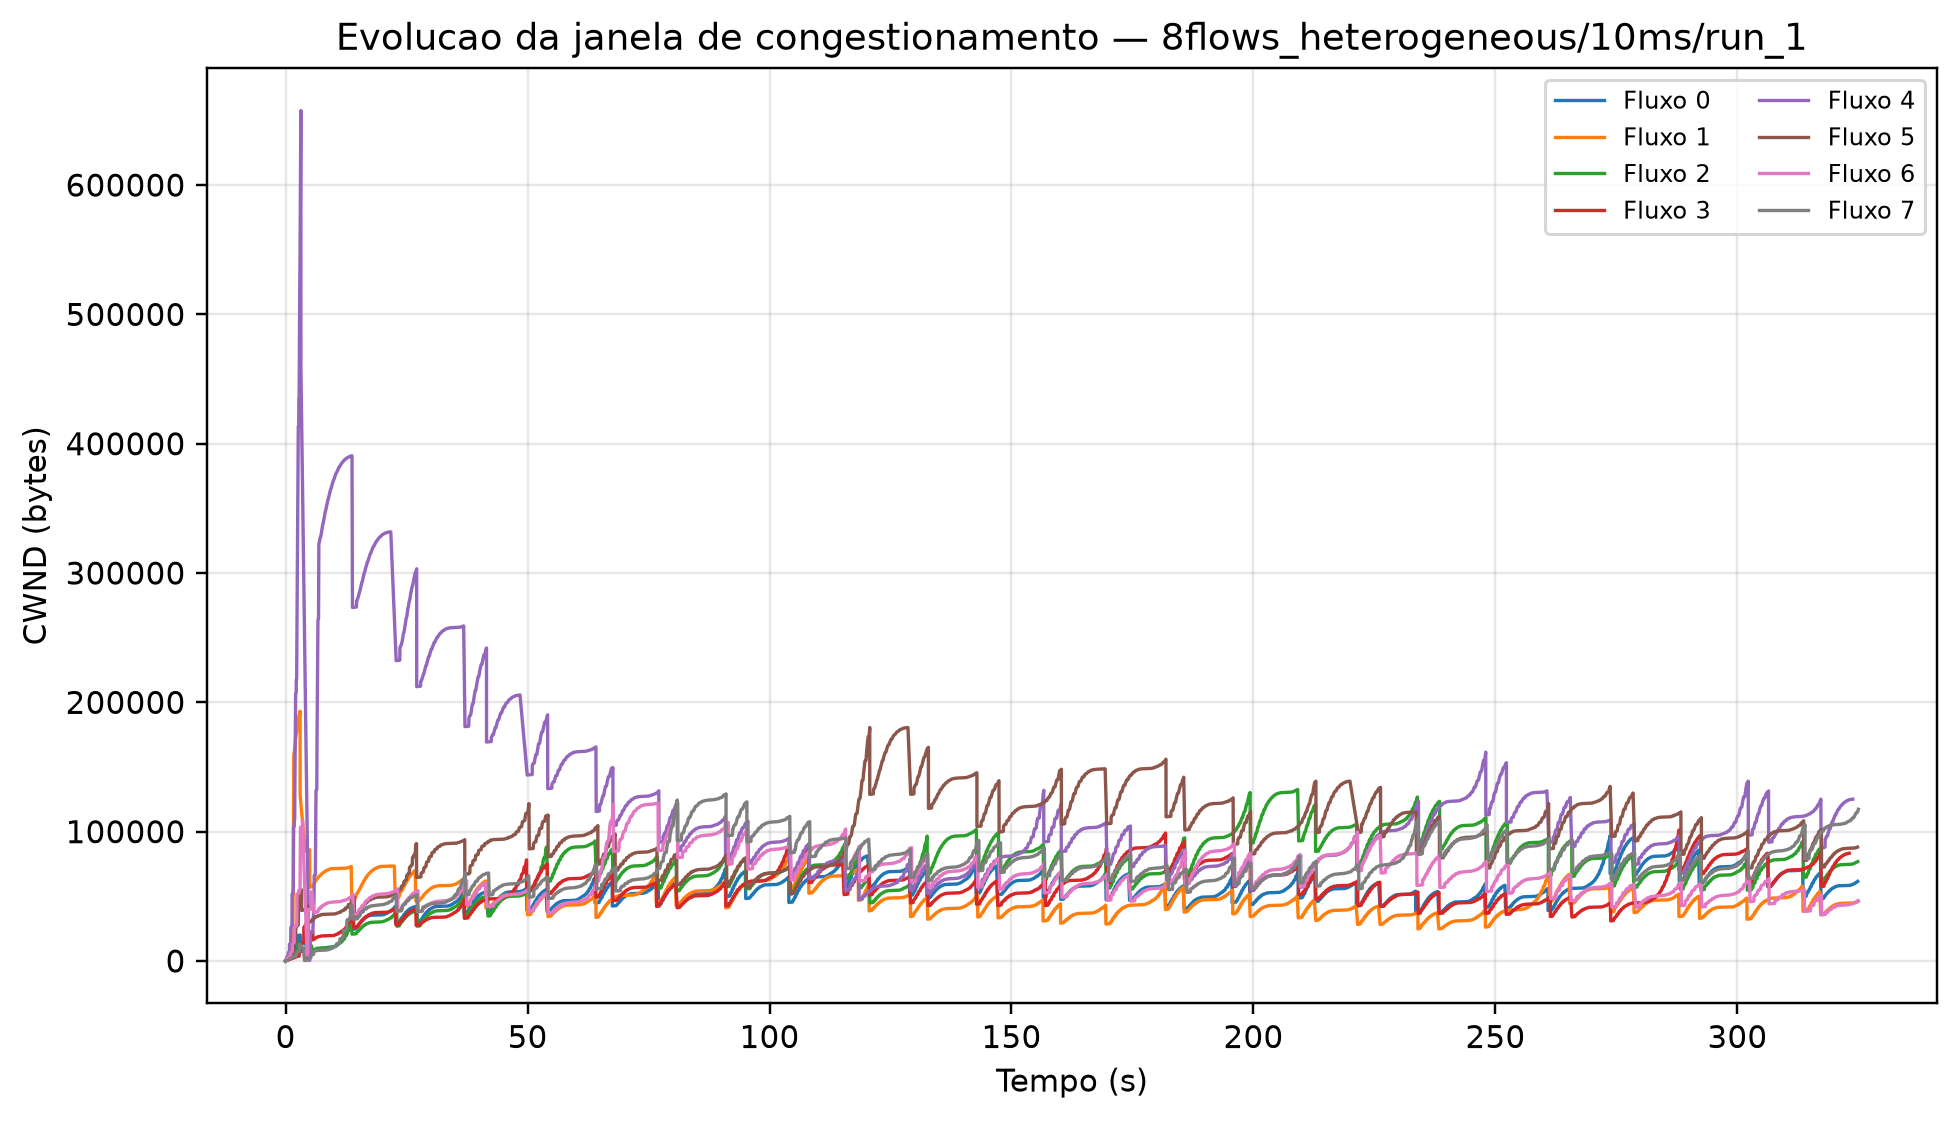
\includegraphics[width=\textwidth]{8flows_heterogeneous_10ms_run_1_cwnd.png}
\caption{Evolução da janela de congestionamento dos oito fluxos, com gargalo de 10 ms.}
\label{fig:trace-cwnd-10}
\end{figure}

\begin{figure}[p]
\centering
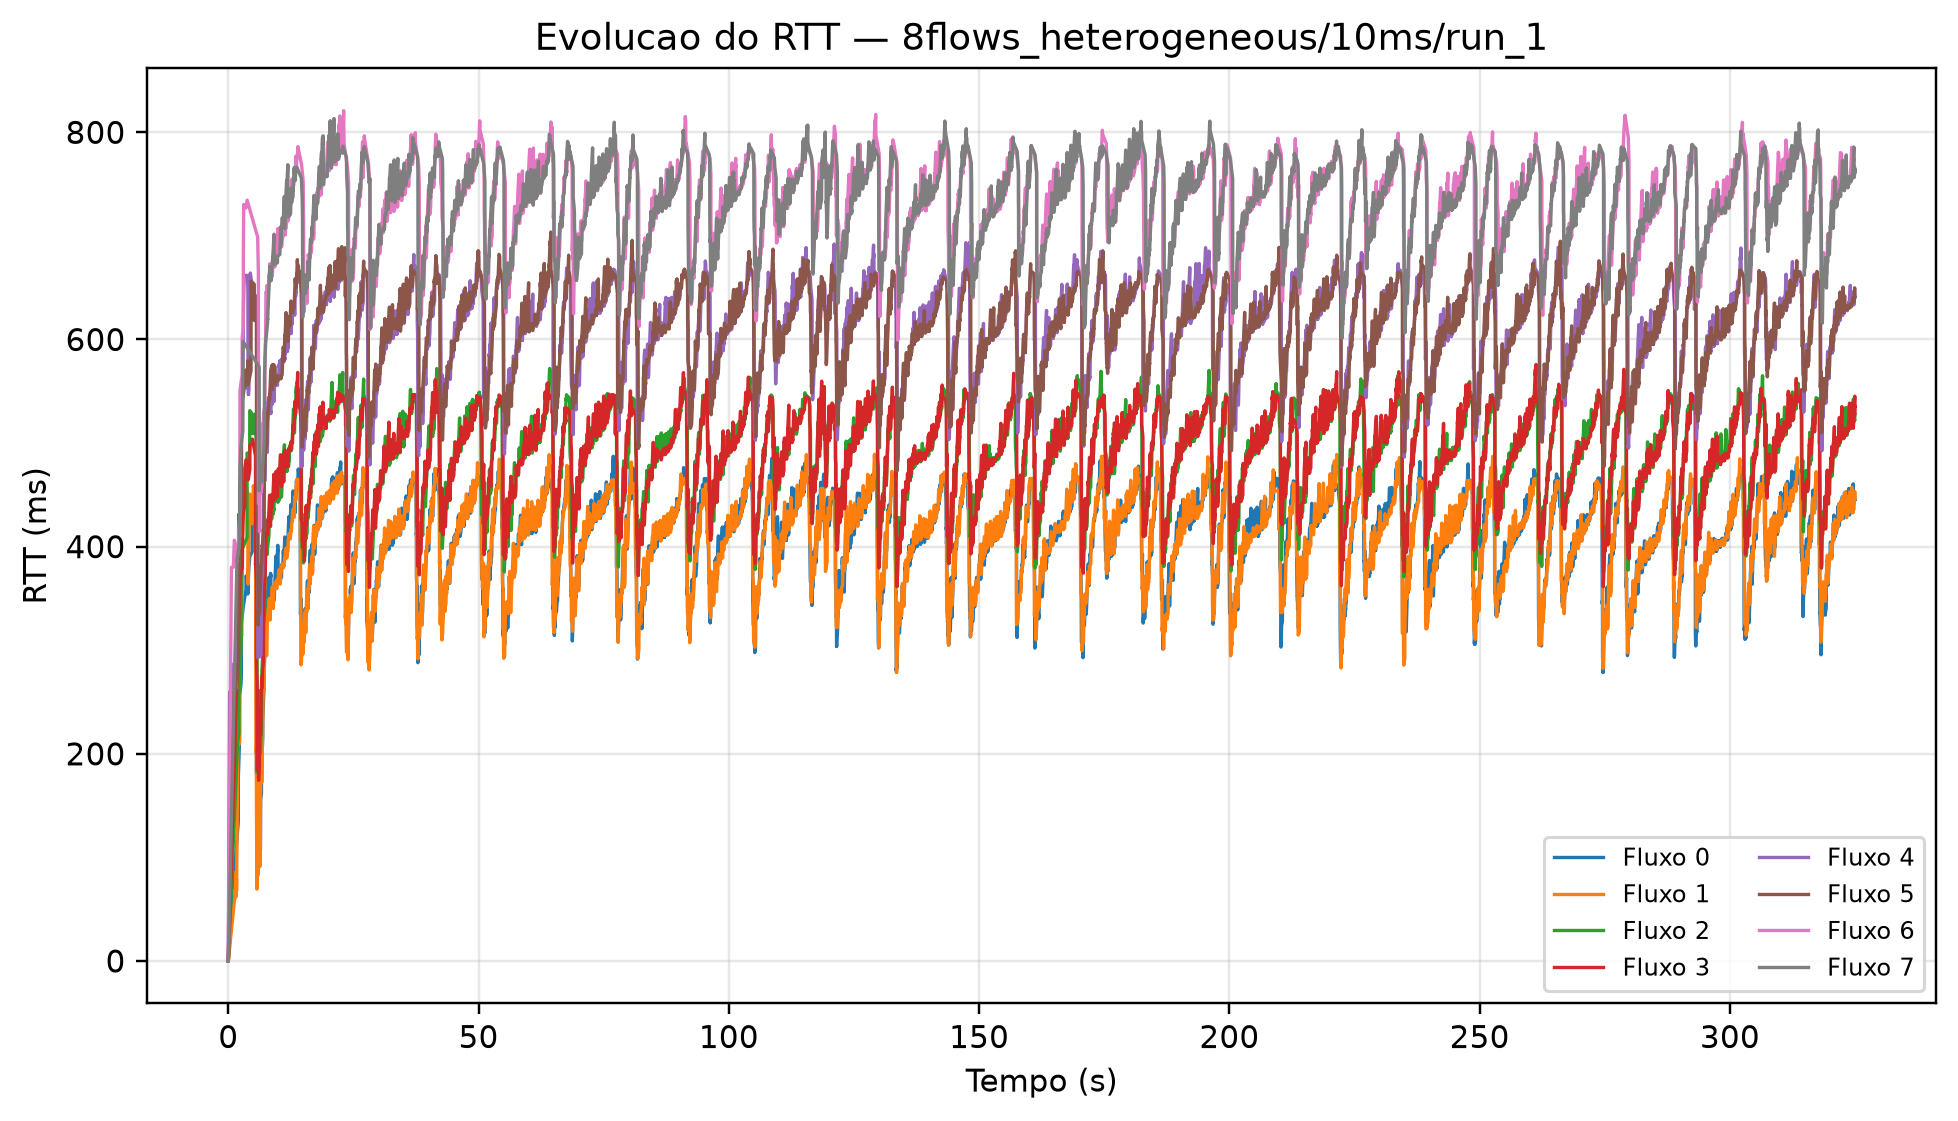
\includegraphics[width=\textwidth]{8flows_heterogeneous_10ms_run_1_rtt.png}
\caption{Evolução do RTT dos oito fluxos, com gargalo de 10 ms.}
\label{fig:trace-rtt-10}
\end{figure}

\section{Atraso de gargalo de 50 ms}

\begin{figure}[p]
\centering
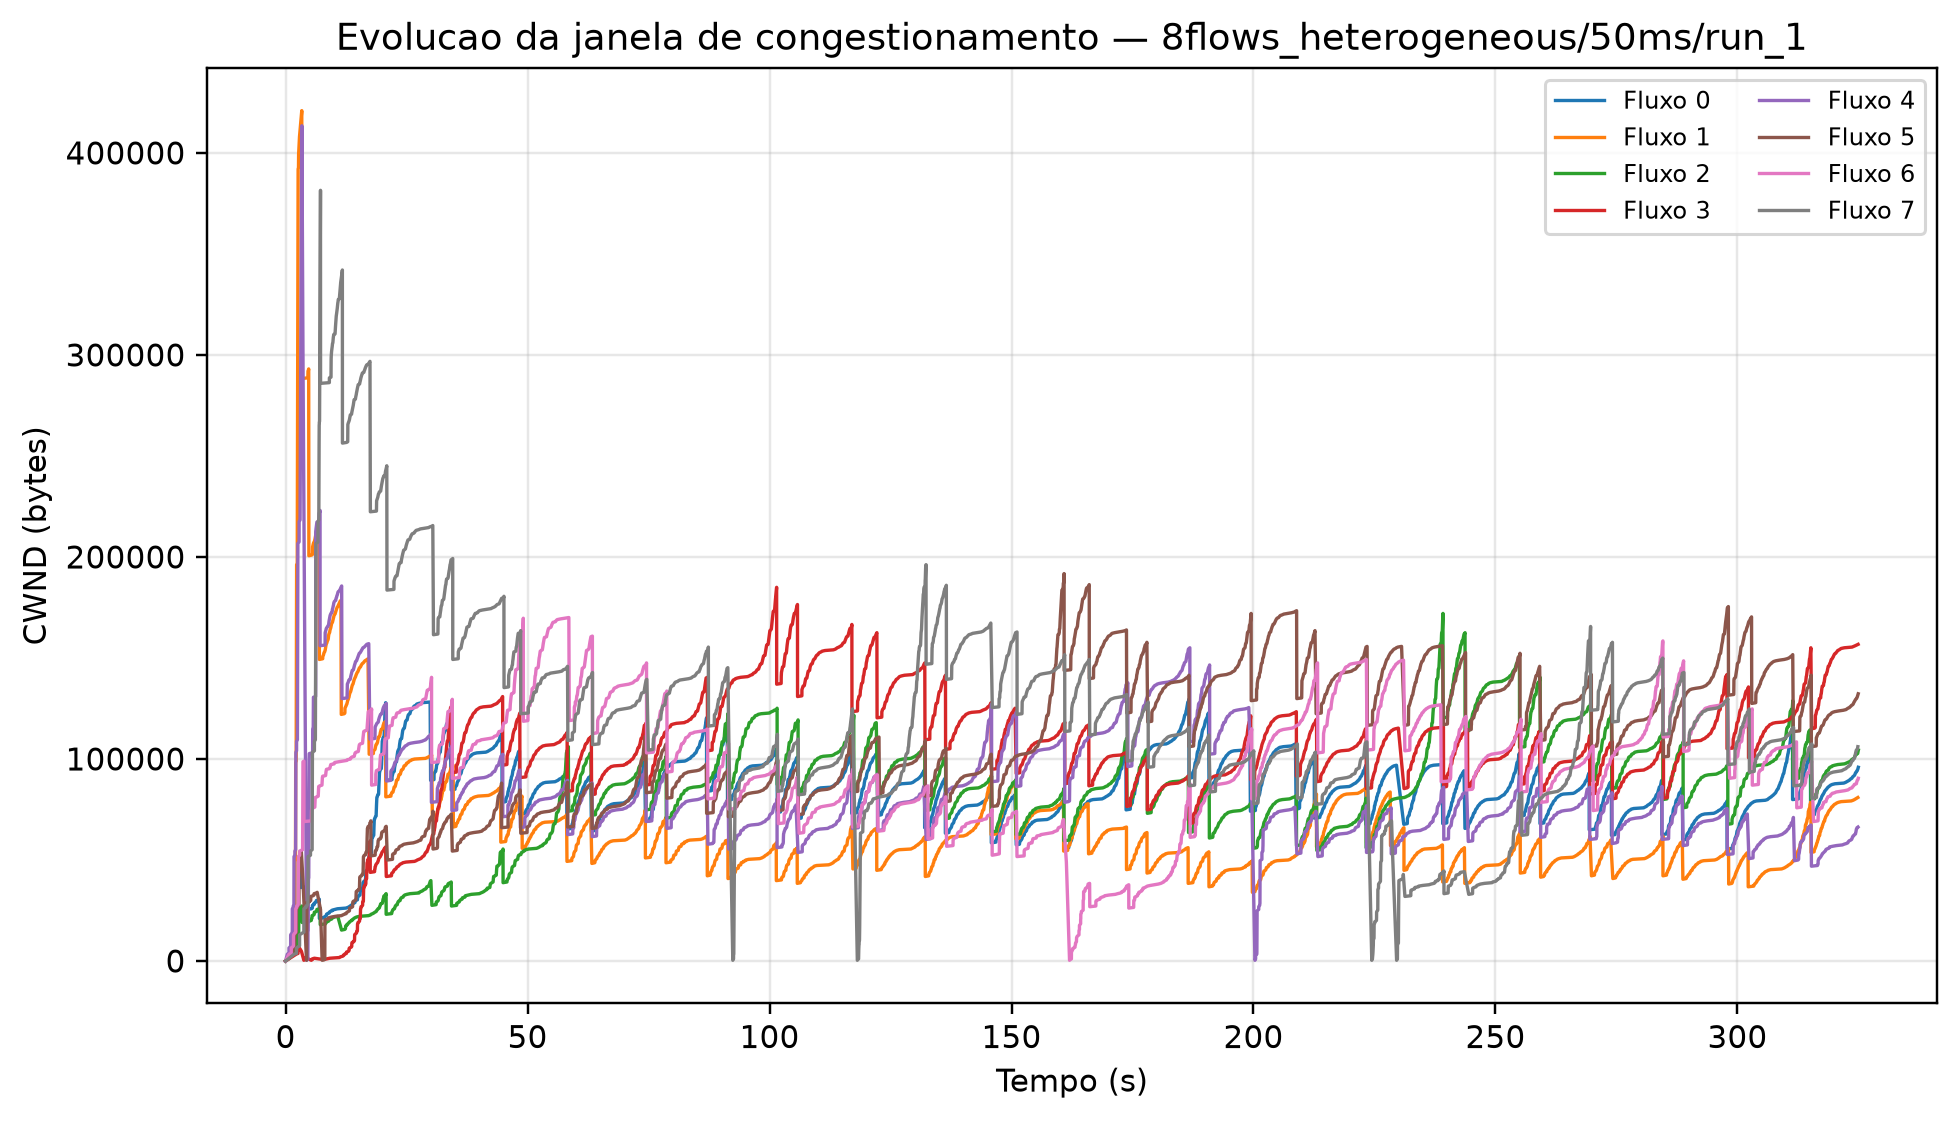
\includegraphics[width=\textwidth]{8flows_heterogeneous_50ms_run_1_cwnd.png}
\caption{Evolução da janela de congestionamento dos oito fluxos, com gargalo de 50 ms.}
\label{fig:trace-cwnd-50}
\end{figure}

\begin{figure}[p]
\centering
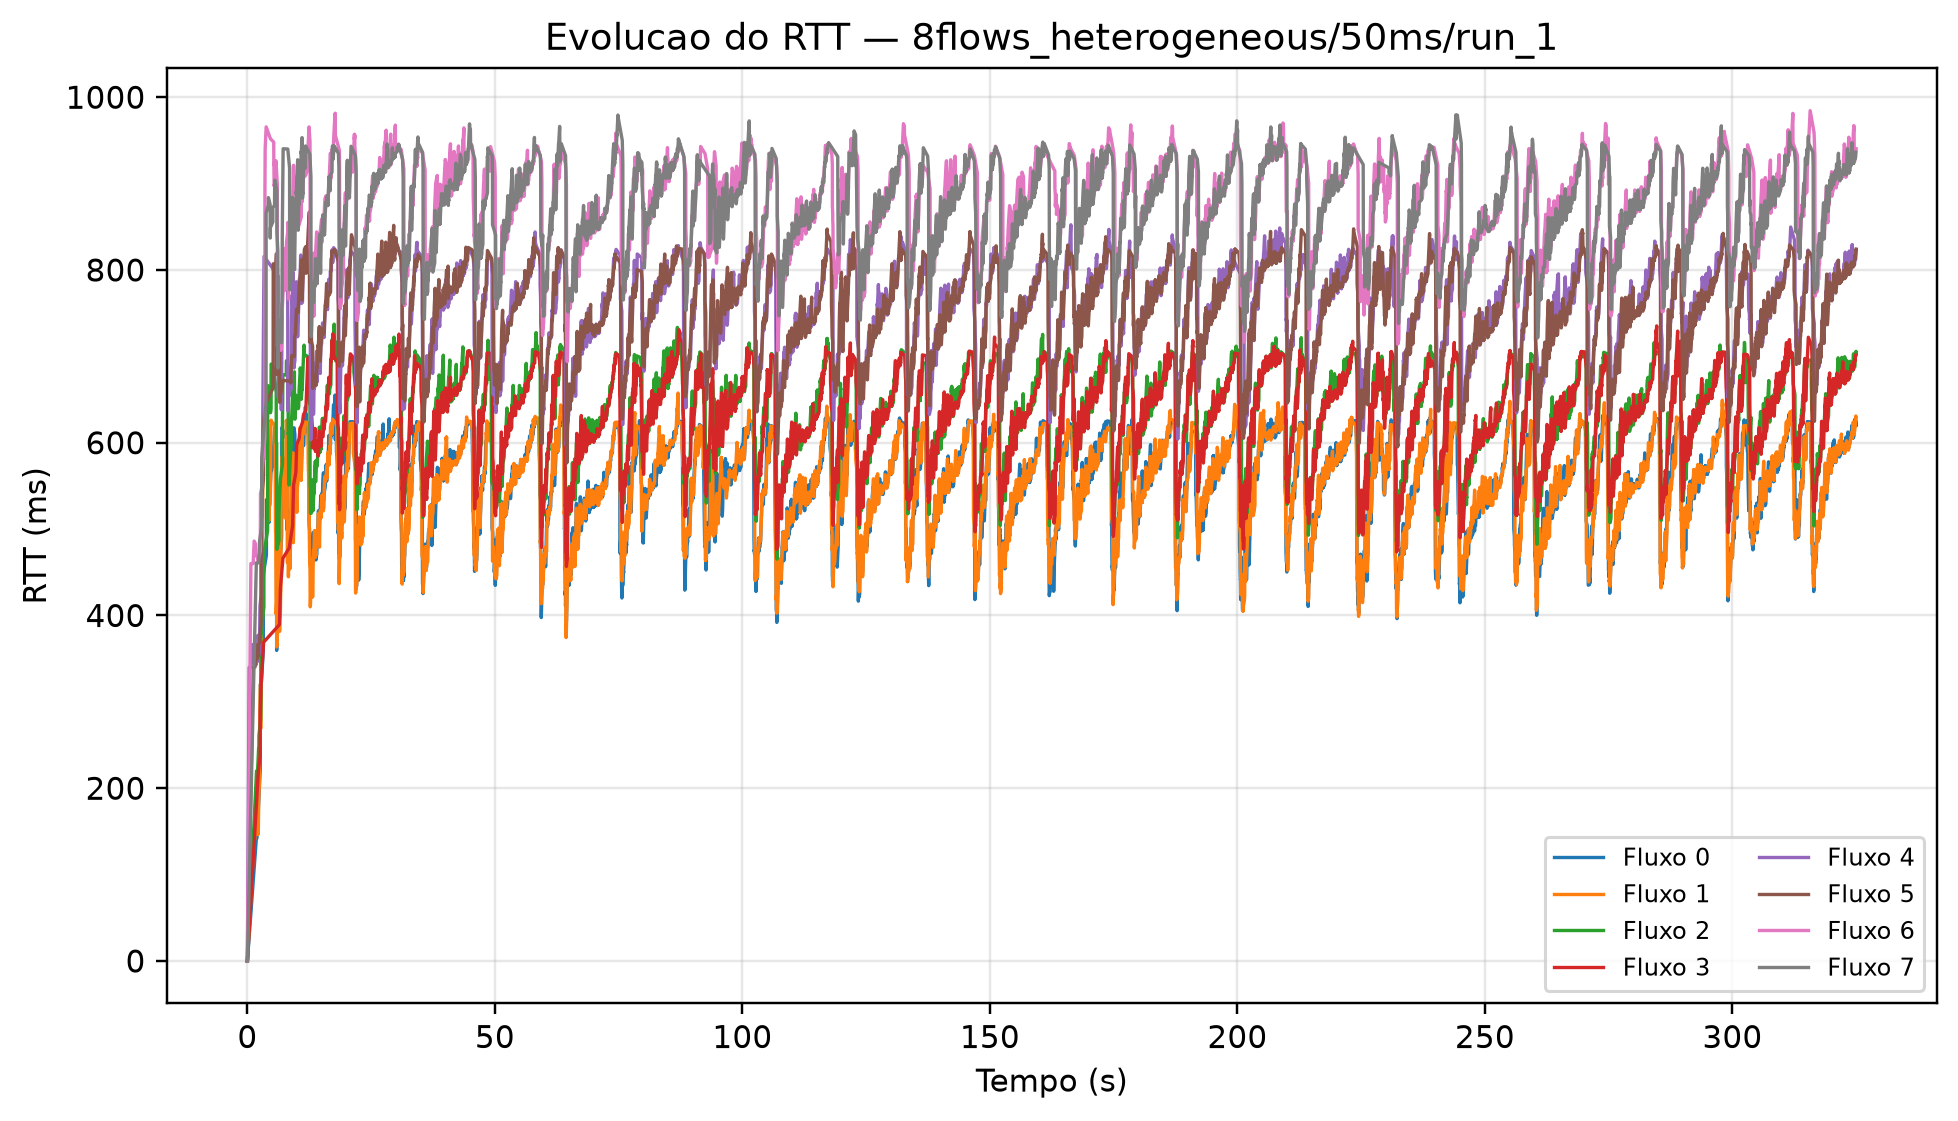
\includegraphics[width=\textwidth]{8flows_heterogeneous_50ms_run_1_rtt.png}
\caption{Evolução do RTT dos oito fluxos, com gargalo de 50 ms.}
\label{fig:trace-rtt-50}
\end{figure}

\section{Atraso de gargalo de 100 ms}

\begin{figure}[p]
\centering
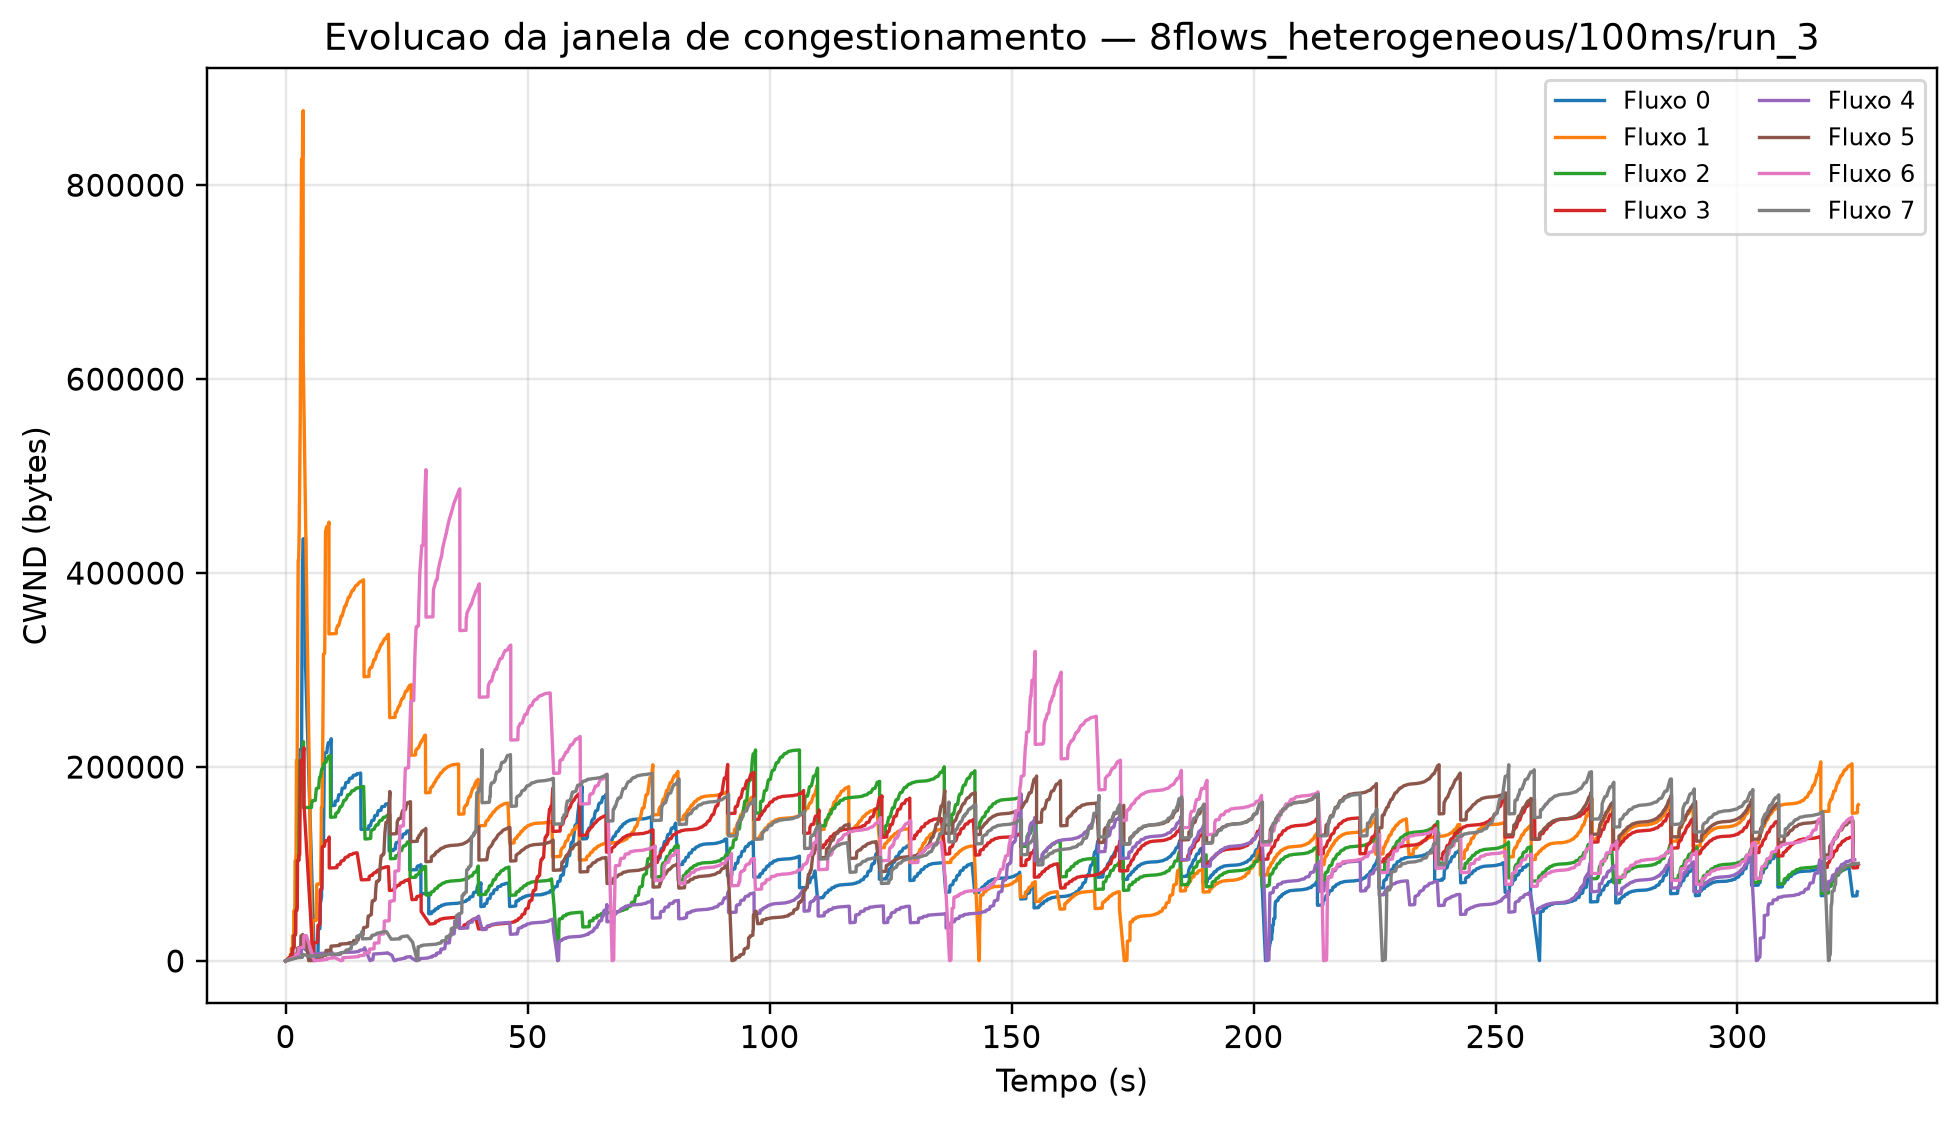
\includegraphics[width=\textwidth]{8flows_heterogeneous_100ms_run_3_cwnd.png}
\caption{Evolução da janela de congestionamento dos oito fluxos, com gargalo de 100 ms.}
\label{fig:trace-cwnd-100}
\end{figure}

\begin{figure}[p]
\centering
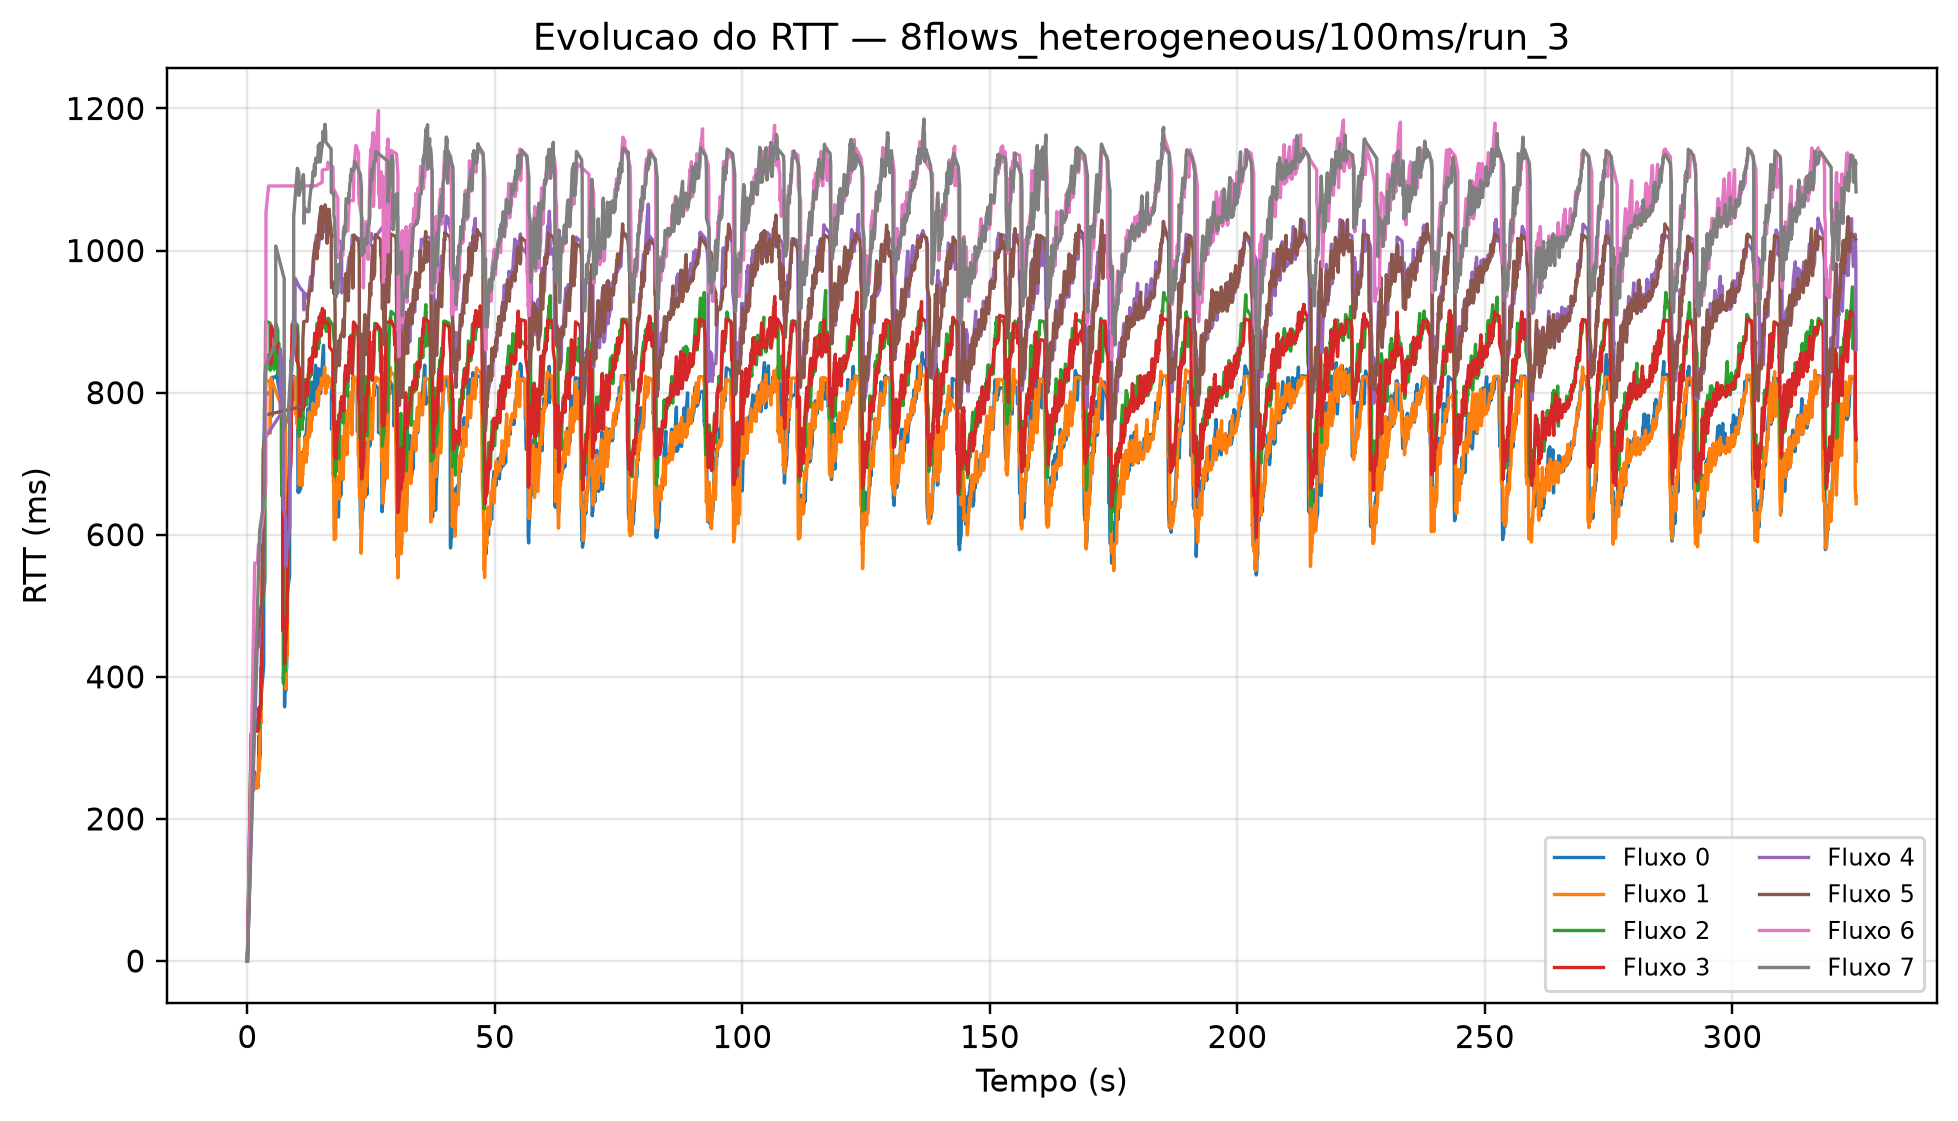
\includegraphics[width=\textwidth]{8flows_heterogeneous_100ms_run_3_rtt.png}
\caption{Evolução do RTT dos oito fluxos, com gargalo de 100 ms.}
\label{fig:trace-rtt-100}
\end{figure}

% --- Referências (ordem alfabética, estilo ABNT) ---


% Referências originais preservadas
e}
    \begin{center}
        {\large \textbf{UNIVERSIDADE FEDERAL DE JUIZ DE FORA}} \\
        {\large \textbf{INSTITUTO DE CIÊNCIAS EXATAS}} \\
        {\large \textbf{BACHARELADO EM CIÊNCIA DA COMPUTAÇÃO}} \\
        
        \vspace{4cm}
        {\large Thales Gomes Batista}
        
        \vspace{2cm}
        {\Large \textbf{Avaliação de uma Proposta de Adaptação do Algoritmo TCP CUBIC Utilizando Informações de RTT}}
        
        \vspace*{\fill}
        {\large Juiz de Fora}\\
        {\large 2026}
    \end{center}
\end{titlepage}

\newpage

% --- 2. Folha de Rosto ---
\begin{titlepage}
    \begin{center}
        {\large Thales Gomes Batista}
        
        \vspace{4cm}
        {\Large \textbf{Avaliação de uma Proposta de Adaptação do Algoritmo TCP CUBIC Utilizando Informações de RTT}}
        
        \vspace{3cm}
        \hspace{.45\textwidth}
        \begin{minipage}{.5\textwidth}
            Trabalho de Conclusão de Curso apresentado ao Instituto de Ciências Exatas da Universidade Federal de Juiz de Fora como requisito parcial à obtenção do grau de bacharel em Ciência da Computação.
            
            \vspace{0.5cm}
            \textbf{Orientador:} Prof. Dr. Edelberto Franco Silva
        \end{minipage}
        
        \vspace*{\fill}
        {\large Juiz de Fora}\\
        {\large 2026}
    \end{center}
\end{titlepage}

\newpage

% --- 3. Agradecimentos ---
\begin{center}
    {\large \textbf{AGRADECIMENTOS}}
\end{center}

\vspace{1cm}
\noindent Agradeço primeiramente à minha família pelo apoio incondicional ao longo de toda a minha trajetória acadêmica e pessoal.

\noindent Agradeço ao meu orientador, Prof. Dr. Edelberto Franco Silva, pela paciência, disponibilidade e orientação técnica fundamentais para a condução desta pesquisa.

\noindent Agradeço aos colegas de curso e à Universidade Federal de Juiz de Fora (UFJF) pelo suporte estrutural e acadêmico durante a graduação.

\newpage

% --- 4. Resumo ---
\begin{center}
    {\large \textbf{RESUMO}}
\end{center}
O controle de congestionamento é fundamental para a eficiência e a estabilidade das redes de computadores, pois regula a quantidade de dados em trânsito e a utilização dos enlaces compartilhados. Este trabalho investiga o comportamento dos algoritmos TCP CUBIC e TCP BBR e, a partir dessa comparação, apresenta uma variante do CUBIC denominada TCP CUBIC-RTT. A proposta incorpora informações relacionadas ao tempo de ida e volta (RTT) à estrutura original do CUBIC, utilizando o menor RTT observado em relação a um valor de referência para adaptar o fator de crescimento cúbico $C$ e o fator de redução multiplicativa $\beta$. Os coeficientes $\alpha$ e $\gamma$ controlam a intensidade dessas adaptações. A implementação foi realizada no simulador ns-3 e avaliada em três campanhas: uma comparação inicial entre CUBIC, BBR e CUBIC-RTT; uma campanha de robustez, com diferentes condições de rede e combinações de parâmetros; e uma campanha de coexistência, na qual quatro fluxos de cada variante compartilham o mesmo gargalo. Foram analisadas vazão, perda de pacotes, atraso médio, jitter e justiça entre fluxos. Na comparação inicial, o CUBIC-RTT manteve vazão agregada próxima à do CUBIC e apresentou jitter ligeiramente menor, mas também atraso médio superior e perda maior em parte dos cenários. Na campanha de coexistência, a vantagem de vazão do CUBIC-RTT aumentou com o atraso do gargalo, indicando que a adaptação pode alterar a distribuição de recursos entre algoritmos concorrentes. Os resultados mostram que a informação de RTT pode modificar o comportamento do CUBIC, mas seus efeitos dependem do cenário e envolvem compromissos entre as métricas avaliadas.

\vspace{1cm}
\noindent \textbf{Palavras-chave:} redes de computadores; controle de congestionamento; TCP CUBIC; TCP BBR; RTT; coexistência de fluxos; ns-3.

\newpage

% --- 5. Abstract ---
\begin{center}
    {\large \textbf{ABSTRACT}}
\end{center}
Congestion control is essential to the efficiency and stability of computer networks because it regulates the amount of data in flight and the use of shared links. This work investigates TCP CUBIC and TCP BBR and, based on this comparison, presents a CUBIC variant named TCP CUBIC-RTT. The proposal incorporates round-trip time (RTT) information into the original CUBIC structure, using the minimum observed RTT relative to a reference value to adapt the cubic growth factor $C$ and the multiplicative reduction factor $\beta$. The coefficients $\alpha$ and $\gamma$ control the intensity of these adaptations. The implementation was developed in the ns-3 simulator and evaluated through three campaigns: an initial comparison among CUBIC, BBR, and CUBIC-RTT; a robustness campaign with different network conditions and parameter combinations; and a coexistence campaign in which four flows of each variant share the same bottleneck. Throughput, packet loss, average delay, jitter, and inter-flow fairness were analysed. In the initial comparison, CUBIC-RTT maintained aggregate throughput close to CUBIC and presented slightly lower jitter, but also higher average delay and higher packet loss in some scenarios. In the coexistence campaign, the throughput advantage of CUBIC-RTT increased with bottleneck delay, indicating that the adaptation can change resource allocation between competing algorithms. The results show that RTT information can modify CUBIC's behaviour, but its effects depend on the scenario and involve trade-offs among the evaluated metrics.

\vspace{1cm}
\noindent \textbf{Keywords:} computer networks; congestion control; TCP CUBIC; TCP BBR; RTT; flow coexistence; ns-3.

\newpage

% --- 6. Listas Automáticas ---
\listoffigures
\newpage

\listoftables
\newpage

% --- 7. Sumário ---
\tableofcontents
\newpage

% ==========================================================
% TEXTO PRINCIPAL
% ==========================================================
\pagenumbering{arabic}

\section{INTRODUÇÃO}
O crescimento contínuo do tráfego de dados e a diversificação das aplicações em tempo real colocam exigências cada vez maiores sobre a infraestrutura das redes de computadores. Nesse cenário, o protocolo de controle de transmissão (\textbf{TCP} --- \textit{Transmission Control Protocol})~\cite{rfc9293} assegura a entrega confiável e ordenada dos dados, mas seu desempenho em enlaces de alta capacidade e com vários fluxos concorrentes depende do \textbf{controle de congestionamento}~\cite{rfc5681}.

Ao longo das décadas, vários algoritmos foram propostos para repartir a largura de banda disponível sem saturar as filas dos roteadores. O \textbf{TCP CUBIC}~\cite{ha2008,rfc9438} tornou-se o algoritmo padrão em sistemas Linux. Em vez de crescer a janela de congestionamento de forma linear, como fazem os algoritmos clássicos da família Reno, o CUBIC usa uma função cúbica do tempo, o que o torna mais escalável em redes de alta velocidade (\textit{high-speed networks}).

O CUBIC, porém, é essencialmente orientado a perdas (\textit{loss-based}): ele só reduz a janela depois que uma perda acontece e, até lá, tende a manter a fila do gargalo cada vez mais cheia. O resultado é o aumento do atraso (\textit{bufferbloat}) e, em alguns casos, prejuízo à justiça (\textit{fairness}) entre fluxos concorrentes. A intensidade desse efeito varia com a topologia, o tamanho dos buffers e o tráfego concorrente, como mostram as comparações experimentais entre CUBIC e BBR~\cite{casas2022,ware2019}.

O \textbf{TCP BBR} (\textit{Bottleneck Bandwidth and Round-trip propagation time}), desenvolvido pelo Google, parte de outra ideia. Em vez de tratar a perda como o principal sinal de congestionamento, ele estima a largura de banda do gargalo e o menor tempo de ida e volta do caminho, e ajusta o envio a partir desse modelo~\cite{cardwell2017}.

Foi dessa diferença de abordagem que nasceu este trabalho, que desenvolve e avalia, no simulador \textbf{ns-3}, uma variante do CUBIC chamada \textbf{TCP CUBIC-RTT}. A proposta usa informações de RTT para ajustar dois parâmetros do algoritmo: o coeficiente $\alpha$, que regula o quanto o crescimento da janela se adapta, e o coeficiente $\gamma$, que regula a redução da janela depois de um congestionamento.

\subsection{JUSTIFICATIVA}
A proposta surgiu da comparação entre a forma como CUBIC e BBR controlam o envio de dados. O CUBIC guia o crescimento da janela por uma função cúbica e reage ao congestionamento principalmente por meio de perdas; o BBR, por sua vez, trabalha com estimativas da largura de banda do gargalo e do RTT de propagação. Dessa diferença veio a pergunta que orienta todo o trabalho: acrescentar uma informação de RTT à lógica do CUBIC muda seu comportamento de forma relevante?

Vale deixar claro que não se parte da premissa de que a adaptação seja melhor do que os algoritmos existentes. Trata-se de uma hipótese a ser testada. Por isso, a proposta mantém a estrutura geral do CUBIC e altera apenas o cálculo de dois fatores, um ligado ao crescimento e outro à redução da janela, usando uma medida de RTT como referência.

A investigação começa com a comparação entre CUBIC, BBR e CUBIC-RTT sob diferentes atrasos no enlace de gargalo. Em seguida, os experimentos são ampliados para variar a largura de banda, a quantidade de fluxos, o atraso dos enlaces de acesso e os coeficientes de adaptação. Avaliar a proposta em condições variadas, e não em um único cenário, acompanha a orientação do RFC 9743~\cite{rfc9743} para a análise de novos algoritmos de controle de congestionamento. São analisadas vazão, perda de pacotes, atraso médio, jitter e justiça entre fluxos.

\subsection{OBJETIVOS}
O objetivo geral é comparar os algoritmos TCP CUBIC e TCP BBR e desenvolver e avaliar uma variante do CUBIC, o TCP CUBIC-RTT, que incorpora uma medida de RTT à adaptação de fatores do controle de congestionamento.

Os objetivos específicos são:
\begin{itemize}
    \item \textbf{Fundamentar} os conceitos de controle de congestionamento em redes TCP, com ênfase no CUBIC, no BBR e nas métricas de avaliação;
    \item \textbf{Comparar inicialmente} CUBIC e BBR em cenários controlados, identificando diferenças de comportamento que motivem a proposta;
    \item \textbf{Implementar} a variante TCP CUBIC-RTT no código-fonte do \texttt{ns-3}, preservando a estrutura geral do CUBIC e introduzindo adaptação baseada em RTT;
    \item \textbf{Executar campanhas experimentais} com diferentes atrasos de gargalo, larguras de banda, quantidades de fluxos, atrasos de acesso e combinações dos coeficientes de adaptação;
    \item \textbf{Coletar e analisar} vazão, perda de pacotes, atraso médio, jitter e justiça entre fluxos, além dos rastros das variáveis internas do TCP;
    \item \textbf{Avaliar criticamente} em quais condições a proposta altera o comportamento do CUBIC e quais compromissos aparecem em relação ao algoritmo original e ao BBR;
    \item \textbf{Investigar a coexistência} entre fluxos CUBIC e CUBIC-RTT que compartilham o mesmo gargalo, verificando se a adaptação favorece ou prejudica uma das variantes.
\end{itemize}

\subsection{ORGANIZAÇÃO DO TRABALHO}
O Capítulo 2 apresenta a fundamentação teórica: o controle de congestionamento no TCP, o CUBIC, o BBR, a simulação por eventos discretos e as métricas de avaliação. O Capítulo 3 descreve a metodologia, com a topologia, as três campanhas experimentais, a matriz de parâmetros e os cuidados estatísticos. O Capítulo 4 detalha a implementação do TCP CUBIC-RTT e as decisões de instrumentação. O Capítulo 5 apresenta e discute os resultados da comparação inicial, da campanha de robustez e do experimento de coexistência. O Capítulo 6 reúne as considerações finais, as contribuições e os trabalhos futuros.

\section{FUNDAMENTAÇÃO TEÓRICA}
O controle de congestionamento é um dos mecanismos mais importantes para a estabilidade da Internet, pois evita o colapso por saturação de roteadores e enlaces. Este capítulo reúne os conceitos necessários para acompanhar o restante do trabalho.

\subsection{Controle de Congestionamento no TCP}
O TCP opera na camada de transporte e oferece um canal confiável e orientado a conexões sobre redes IP que, em geral, só fazem entrega pelo melhor esforço (\textit{best-effort})~\cite{rfc9293,kurose2017}. Para que os emissores não sobrecarreguem roteadores cujos buffers são finitos, o TCP mantém uma janela de congestionamento (\textit{congestion window}, $cwnd$) que limita a quantidade de dados em trânsito (\textit{bytes in flight}) antes da chegada das confirmações (\textit{ACKs}). O limiar de partida lenta (\textit{slow start threshold}, $ssthresh$) define quando a janela deixa de crescer de forma exponencial e passa a crescer de forma mais cautelosa~\cite{rfc5681}.

Algoritmos clássicos como o TCP Reno seguem o esquema AIMD (\textit{Additive Increase, Multiplicative Decrease}): a janela cresce linearmente a cada RTT e é reduzida pela metade diante de uma perda~\cite{rfc5681,kurose2017}. Esse esquema é robusto, mas se mostra ineficiente em redes de alta velocidade e alto produto largura de banda-atraso (\textit{Bandwidth-Delay Product}, BDP), porque a janela leva muito tempo para se recuperar depois de uma perda.

\subsection{O Algoritmo TCP CUBIC}
O TCP CUBIC foi proposto para corrigir essa limitação em redes de alta velocidade~\cite{ha2008}. Em vez de crescer linearmente, a janela é função cúbica do tempo $t$ decorrido desde a última redução~\cite{rfc9438}:
\begin{equation}
    W_{cubic}(t) = C\,(t-K)^3 + W_{max}, \qquad K = \sqrt[3]{\frac{W_{max}\,(1-\beta)}{C}}
\end{equation}
onde $W_{max}$ é a janela registrada imediatamente antes da última redução, $C$ é o fator de escala do crescimento cúbico, $\beta$ é a fração da janela preservada após uma perda e $K$ é o tempo que a função leva para voltar a $W_{max}$. A especificação atual adota $C=0{,}4$ e $\beta=0{,}7$~\cite{rfc9438}.

O formato da curva explica o comportamento do algoritmo. Logo após uma redução, a janela cresce depressa; ao se aproximar de $W_{max}$, o crescimento desacelera, o que dá estabilidade a esse ponto; ultrapassado $W_{max}$, a curva volta a acelerar para sondar se há capacidade adicional. Como o crescimento depende do tempo e não do RTT, o CUBIC é adequado a caminhos de longa distância.

Por reagir sobretudo a perdas, o CUBIC pode deixar a fila do gargalo crescer antes de perceber o congestionamento, o que eleva a latência e favorece o \textit{bufferbloat}. O tamanho desse efeito depende da topologia, dos buffers, da capacidade dos enlaces e da concorrência entre fluxos.

\subsection{O Algoritmo TCP BBR}
O TCP BBR~\cite{cardwell2017} segue uma abordagem baseada em modelo. Ele estima continuamente a largura de banda máxima do gargalo ($BtlBw$, \textit{bottleneck bandwidth}) e o tempo mínimo de propagação do RTT ($RTprop$). Com essas estimativas, calcula o BDP e regula a taxa de envio e a quantidade de dados em trânsito para usar a capacidade do gargalo sem manter filas longas.

Esse mecanismo não garante ausência de filas ou perdas. O desempenho e a justiça do BBR variam com a versão do algoritmo, o tamanho dos buffers, a topologia e a presença de outros fluxos, inclusive fluxos CUBIC~\cite{ware2019,casas2022}.

\subsection{Simulação de Redes por Eventos Discretos no ns-3}
Experimentos em redes físicas costumam ser difíceis de reproduzir e de isolar variável por variável. Por isso, recorre-se a simuladores de eventos discretos, entre os quais o \textbf{ns-3}~\cite{ns3}. O \texttt{ns-3} é um simulador de código aberto escrito em C++ (com \textit{bindings} para Python) que modela a pilha de protocolos IP, canais, enlaces e algoritmos de controle de tráfego. Sua arquitetura modular permite implementar novas variantes de transporte e executar cenários controlados e repetíveis, requisito importante para a pesquisa acadêmica.

\subsection{Métricas de Avaliação de Desempenho}
O comportamento dos protocolos de transporte é analisado com um conjunto de métricas de qualidade de serviço:
\begin{itemize}
    \item \textbf{Vazão (\textit{throughput}):} taxa de dados úteis entregues ao destino por unidade de tempo, em Mbps.
    \item \textbf{Atraso médio unidirecional:} intervalo entre o envio de um pacote e sua recepção no destino, conforme o FlowMonitor. Não deve ser confundido com o RTT, que é o tempo de ida e volta observado pela conexão.
    \item \textbf{Taxa de perda de pacotes:} percentual de pacotes descartados no caminho por congestionamento e estouro de filas.
    \item \textbf{Jitter:} média das variações absolutas entre os atrasos de pacotes consecutivos, conforme os registros do FlowMonitor. A noção de variação de atraso de pacotes é a mesma formalizada na métrica IPDV do IETF~\cite{rfc3393}; aqui, porém, vale a definição operacional do FlowMonitor.
    \item \textbf{Índice de Justiça de Jain:} medida adimensional da equidade na divisão de recursos entre $n$ fluxos~\cite{jain1984}, dada por
    \begin{equation}
        J = \frac{\left( \sum_{i=1}^{n} x_i \right)^2}{n \sum_{i=1}^{n} x_i^2}
    \end{equation}
    em que $x_i$ é a vazão média do $i$-ésimo fluxo. O índice varia em $[1/n, 1]$, e valores próximos de $1$ indicam distribuição mais equilibrada.
\end{itemize}

\section{METODOLOGIA}

A metodologia combina o desenvolvimento da variante TCP CUBIC-RTT com sua avaliação experimental. A abordagem é empírico-quantitativa: simulações no ns-3 comparam o comportamento da proposta com o do CUBIC e do BBR. O processo teve as seguintes etapas: implementação da proposta, definição das topologias e dos parâmetros, execução das campanhas, coleta das métricas e processamento dos dados.

\subsection{Ambiente de Simulação}

Os experimentos foram realizados no simulador ns-3~\cite{ns3}, que permite controlar as características dos enlaces, os atrasos de propagação, a largura de banda e a quantidade de fluxos concorrentes. Com isso, os algoritmos são comparados em condições experimentais equivalentes.

Os cenários foram implementados em C++ sobre os módulos de rede e transporte do ns-3. Para registrar o comportamento dos fluxos, usaram-se mecanismos de rastreamento de eventos e o módulo FlowMonitor.

\subsection{Arquitetura da Topologia Experimental}

A topologia tem dois roteadores intermediários, Gateway A e Gateway B, ligados por um enlace compartilhado que é o gargalo da rede. Os nós de origem abrem fluxos TCP que atravessam o Gateway A, passam pelo gargalo e chegam aos nós de destino pelo Gateway B. Dessa forma, vários fluxos disputam a capacidade de um mesmo enlace, o que permite observar como cada algoritmo se comporta sob competição por recursos.

A largura de banda e o atraso de propagação do gargalo são configuráveis. Os enlaces de acesso dos nós finais têm parâmetros próprios, mantidos fixos em cada cenário, de modo que a variação analisada venha principalmente do gargalo e da quantidade de fluxos.

\subsection{Parâmetros e Variáveis Experimentais}

Os experimentos foram organizados em três campanhas complementares. A primeira compara TCP CUBIC, TCP BBR e TCP CUBIC-RTT em uma topologia controlada. A segunda amplia a avaliação, variando os parâmetros da proposta e as condições de rede. A terceira investiga a coexistência entre fluxos CUBIC e CUBIC-RTT no mesmo gargalo. A ampliação dos cenários segue a orientação de avaliar novos algoritmos sob condições diversas de rede~\cite{rfc9743}.

\subsubsection{Campanha Comparativa Inicial}

Os parâmetros comuns da campanha inicial são:

\begin{itemize}
    \item Largura de banda do gargalo: 2 Mbps;
    \item Largura de banda dos enlaces de acesso: 10 Mbps;
    \item Atraso dos enlaces de acesso: 45 ms;
    \item Número de fluxos concorrentes: 4;
    \item Duração de cada simulação: 100 segundos;
    \item Número de repetições: 5;
    \item Atrasos do gargalo: 10 ms, 50 ms e 100 ms.
\end{itemize}

Com três algoritmos, três atrasos e cinco repetições, a campanha compreende 45 execuções.

\subsubsection{Campanha de Robustez e Variação de Parâmetros}
\label{sec:robustez}

A segunda campanha investiga o comportamento dos algoritmos sob outras condições de rede e com diferentes configurações do CUBIC-RTT. Foram definidos três cenários:

\begin{itemize}
    \item \textbf{bw1\_f4:} gargalo de 1 Mbps, quatro fluxos e atraso de acesso de 45 ms;
    \item \textbf{bw2\_f8:} gargalo de 2 Mbps, oito fluxos e atraso de acesso de 45 ms;
    \item \textbf{access100:} gargalo de 2 Mbps, quatro fluxos e atraso de acesso de 100 ms.
\end{itemize}

Em todos os cenários, os enlaces de acesso têm 10 Mbps. Os atrasos do gargalo voltam a ser 10 ms, 50 ms e 100 ms, com cinco repetições por configuração.

A campanha contempla quinze configurações de algoritmo e parâmetros: o CUBIC original, o BBR, o CUBIC-RTT na configuração de referência ($\alpha=0{,}25$ e $\gamma=0{,}05$) e doze configurações adicionais do CUBIC-RTT, obtidas pela variação de $\alpha$ e $\gamma$:

\begin{itemize}
    \item $\alpha=0{,}10$: $\gamma \in \{0{,}00; 0{,}025; 0{,}05; 0{,}10\}$;
    \item $\alpha=0{,}25$: $\gamma \in \{0{,}00; 0{,}025\}$;
    \item $\alpha=0{,}50$: $\gamma \in \{0{,}00; 0{,}025\}$;
    \item $\alpha=0{,}75$: $\gamma \in \{0{,}00; 0{,}025; 0{,}05; 0{,}10\}$.
\end{itemize}

O total de execuções da campanha é

\begin{equation}
N = 3 \times 15 \times 3 \times 5 = 675.
\end{equation}

Separar as campanhas permite avaliar primeiro os algoritmos tradicionais e a proposta e, depois, a influência dos parâmetros internos do CUBIC-RTT em cenários mais diversos.

\subsubsection{Campanha de Coexistência entre CUBIC e CUBIC-RTT}

A terceira campanha foi concebida para observar diretamente a interação entre as duas variantes quando disputam a mesma capacidade de transmissão. Foram executados oito fluxos TCP simultâneos: os fluxos 0, 2, 4 e 6 utilizaram CUBIC, enquanto os fluxos 1, 3, 5 e 7 utilizaram CUBIC-RTT, com $\alpha=0{,}25$ e $\gamma=0{,}05$. A alternância foi mantida também na atribuição dos enlaces de acesso, de modo que cada algoritmo tivesse um fluxo em cada uma das quatro condições de atraso de acesso.

O gargalo compartilhado foi configurado com largura de banda de 10 Mbps e atrasos de 10 ms, 50 ms e 100 ms. Os enlaces de acesso operaram a 1 Gbps e foram configurados com atrasos de 10 ms, 30 ms, 60 ms e 90 ms, cada condição atribuída a um par de fluxos, um de cada algoritmo. O experimento utilizou aquecimento de 20 segundos, seguido por 300 segundos de medição, cinco repetições por atraso e início dos fluxos com deslocamento aleatório de até dois segundos. A configuração de fila utilizou um tamanho equivalente a um BDP.

Assim, a campanha compreendeu:
\begin{equation}
N_{\text{coexistência}} = 3 \times 5 = 15
\end{equation}
execuções, totalizando 120 registros de fluxos de dados no FlowMonitor. A vazão foi comparada pela média dos quatro fluxos de cada algoritmo em cada repetição. A perda foi consolidada a partir dos pacotes transmitidos e perdidos, enquanto atraso e jitter foram calculados a partir dos valores dos quatro fluxos de cada grupo.

A atribuição dos algoritmos foi conferida pelos endereços de origem: os endereços \texttt{10.0.1.1}, \texttt{10.0.3.1}, \texttt{10.0.5.1} e \texttt{10.0.7.1} identificam os fluxos CUBIC; os endereços \texttt{10.0.2.1}, \texttt{10.0.4.1}, \texttt{10.0.6.1} e \texttt{10.0.8.1} identificam os fluxos CUBIC-RTT. Essa separação permite observar se a vantagem de uma variante ocorre sem confundir os resultados com a diferença de atraso dos enlaces de acesso.

\subsubsection{Execução e consolidação das campanhas}

As três campanhas totalizam 735 simulações: 45 na comparação inicial, 675 na campanha de robustez e 15 na campanha de coexistência. Nas duas primeiras campanhas, cada simulação contém quatro fluxos nos cenários \texttt{bw1\_f4} e \texttt{access100}, e oito fluxos no cenário \texttt{bw2\_f8}. A campanha de coexistência utiliza oito fluxos em todas as execuções.

Como o FlowMonitor registra fluxos nos dois sentidos da comunicação, os registros foram processados para separar os fluxos de dados das conexões reversas utilizadas para os reconhecimentos (ACKs). Essa filtragem evita contabilizar o tráfego de retorno como se fosse tráfego útil independente. Nas duas primeiras campanhas, foram consolidados 3.780 registros de fluxos de dados. A campanha de coexistência acrescentou 120 registros, correspondentes a oito fluxos em cada uma das quinze execuções.

Os rastros internos também foram auditados. Os 3.780 arquivos de CWND e os 3.780 de SSThresh (7.560 no total) estavam completos, sem pares ausentes, erros ou avisos. Nos dados do FlowMonitor, os totais de bytes e pacotes transmitidos e recebidos foram confirmados, e a taxa de perda e o atraso médio foram reproduzidos exatamente a partir dos valores brutos. O recálculo do jitter apresentou erro médio de cerca de $5{,}57\times10^{-6}$ ms (máximo de $2{,}03\times10^{-4}$ ms), e o índice de Jain, diferença média de aproximadamente 0,00028 (máxima de 0,00349), atribuídas à precisão numérica e à forma de agregação por fluxo. Por serem muito pequenas, essas diferenças não alteram a interpretação dos resultados.

A aleatoriedade das simulações foi controlada pelas sementes do ns-3: todas as execuções usam $Seed = 1$, e o identificador de repetição \texttt{RngRun} assume valores de 1 a 5. Assim, as condições de cada repetição podem ser reproduzidas, desde que se mantenham as versões do código, os parâmetros e a configuração dos geradores.

Há, porém, uma ressalva importante. Identificadores diferentes não garantem independência estatística, pois alguns algoritmos se comportam de forma determinística em condições idênticas. Foi o que se observou na campanha inicial: CUBIC e CUBIC-RTT produziram valores idênticos entre repetições em algumas métricas, enquanto o BBR variou. Por isso, médias e desvios são tratados como estatísticas descritivas das execuções, e não como base para afirmar significância estatística onde não há variabilidade efetiva.

\subsection{Coleta das Métricas de Desempenho}

Os dados foram coletados por dois mecanismos complementares: o FlowMonitor e o rastreamento de variáveis internas do TCP.

\subsubsection{Métricas obtidas pelo FlowMonitor}

O FlowMonitor forneceu, para cada fluxo:

\begin{itemize}
    \item \textbf{Vazão:} dados recebidos com sucesso por unidade de tempo, em Mbps;
    \item \textbf{Perda de pacotes:} relação entre os pacotes transmitidos e os que não chegaram ao destino;
    \item \textbf{Atraso médio:} média dos atrasos dos pacotes recebidos;
    \item \textbf{Jitter:} variação dos atrasos entre pacotes consecutivos.
\end{itemize}

As métricas foram analisadas por fluxo e de forma agregada por simulação, considerando os totais e os intervalos de tempo do conjunto de fluxos. O RTT, por sua vez, é analisado à parte, a partir do rastreamento da variável interna do TCP.

\subsubsection{Métricas internas do TCP}

Foram rastreadas quatro variáveis internas, o que permite observar a evolução do controle de congestionamento ao longo do tempo:

\begin{itemize}
    \item \textbf{CWND:} janela de congestionamento do emissor, em bytes;
    \item \textbf{SSThresh:} limiar de transição entre as fases de crescimento da janela;
    \item \textbf{RTT:} tempo de ida e volta observado pela conexão;
    \item \textbf{InFlight:} quantidade de dados enviados e ainda não reconhecidos.
\end{itemize}

\subsection{Processamento e Consolidação dos Dados}

Os arquivos gerados são organizados por algoritmo, cenário, atraso e repetição. Scripts em Python leem os arquivos, identificam os fluxos relevantes, calculam estatísticas e consolidam os resultados em arquivos CSV. O processamento associa as métricas de cada fluxo ao respectivo cenário e verifica a consistência dos dados: registros ausentes, duplicações e divergências entre totais agregados e valores individuais.

A justiça na distribuição da banda foi avaliada com o Índice de Jain~\cite{jain1984}, calculado a partir da vazão ou da quantidade de dados recebida pelos fluxos, conforme a análise.

\subsection{Tratamento Estatístico e Limitações das Repetições}

Os resultados são organizados por configuração e repetição. Quando há variabilidade entre as execuções, usam-se medidas descritivas (média, mínimo e máximo). Algumas configurações, no entanto, podem produzir execuções idênticas, sobretudo quando algoritmo e cenário não introduzem variação aleatória efetiva entre as repetições, e a interpretação dos resultados considera essa possibilidade.

\section{IMPLEMENTAÇÃO DO TCP CUBIC-RTT}

O TCP CUBIC-RTT foi implementado diretamente no código-fonte do ns-3, a partir do TCP CUBIC que o simulador já oferece. A implementação está nos arquivos \texttt{tcp-cubic-rtt.cc} e \texttt{tcp-cubic-rtt.h}.

A ideia central é incorporar informações de RTT ao crescimento e à redução da janela do CUBIC. Para isso, foram introduzidos dois coeficientes de sensibilidade, $\alpha$ e $\gamma$, que controlam a intensidade da adaptação do fator de crescimento cúbico $C$ e do fator de redução multiplicativa $\beta$ após o congestionamento.

\subsection{Estrutura Geral da Modificação}

O CUBIC original usa uma função cúbica para determinar o crescimento da janela, com parâmetros que definem a velocidade e a forma desse crescimento. No CUBIC-RTT, o fator de escala cúbico deixa de ser fixo e passa a ser ajustado conforme o RTT observado pela conexão. De forma análoga, o fator de redução multiplicativa usado após a detecção de perdas também passa a considerar a condição de atraso. A estrutura geral do CUBIC é mantida: a adaptação entra apenas nos pontos que calculam o crescimento e o limiar de congestionamento.

\subsection{Adaptação Baseada no RTT}

O mecanismo se apoia em duas grandezas: o menor RTT observado pela conexão, \texttt{m\_delayMin}, e um RTT de referência, \texttt{m\_rttReference}, fixado em 200 ms na configuração de referência dos experimentos. Note que a variável usada é o mínimo observado, e não a amostra instantânea de RTT. A referência serve de ponto de comparação: ela indica se o atraso mínimo da conexão está acima ou abaixo do nível considerado adequado.

A razão entre os dois valores é
\begin{equation}
rttRatio = \frac{m\_delayMin}{m\_rttReference}
\end{equation}
e sua diferença em relação à referência é normalizada e limitada ao intervalo $[-1, 1]$:
\begin{equation}
x = clamp(rttRatio - 1.0, -1.0, 1.0)
\end{equation}

Esse limite evita que RTTs extremos provoquem alterações desproporcionais nos parâmetros adaptativos. Se o menor RTT observado fica abaixo da referência, $x$ é negativo; se a ultrapassa, $x$ é positivo. Como a formulação parte do valor mínimo, ela mede a relação entre o atraso mínimo da conexão e a referência configurada e, por isso, não detecta aumentos transitórios de RTT causados pelo enfileiramento.

\subsection{Adaptação do Fator de Crescimento Cúbico}

O primeiro mecanismo atua sobre o fator $C$, que controla a agressividade do crescimento da janela. O fator adaptativo é
\begin{equation}
C_{adaptive} =
m\_c \times (1.0 + m\_alpha \times x)
\end{equation}
onde $m\_c$ é o fator cúbico original, $m\_alpha$ é o coeficiente $\alpha$ de sensibilidade ao RTT e $x$ é a variação normalizada do RTT em relação à referência. Quanto maior o valor de $\alpha$, maior a influência de $x$ sobre $C$; valores menores produzem uma adaptação mais moderada. Variar $\alpha$ permite, desse modo, investigar diferentes níveis de sensibilidade do crescimento da janela ao atraso da rede.

\subsection{Adaptação do Fator de Redução Multiplicativa}

O segundo mecanismo atua sobre o fator $\beta$, que define a proporção da janela mantida após um evento de perda:
\begin{equation}
\beta_{calc} =
m\_beta + m\_gamma \times x
\end{equation}
Para que o resultado respeite os limites da implementação, aplica-se uma função de limitação:
\begin{equation}
\beta_{adaptive} =
clamp(\beta_{calc}, m\_betaMin, m\_betaMax)
\end{equation}

O coeficiente $\gamma$ determina, assim, a influência de $x$ sobre o fator multiplicativo. Como $\beta$ é a fração da janela preservada, valores maiores correspondem a uma redução menos acentuada e valores menores, a uma redução mais forte.

As duas equações devem ser lidas em conjunto. Quando $x$ é positivo, tanto $C_{adaptive}$ quanto $\beta_{adaptive}$ tendem a aumentar: o crescimento cúbico fica mais intenso e uma fração maior da janela é preservada após a perda. Quando $x$ é negativo, ocorre o contrário. Não se pode afirmar, portanto, que todo aumento de RTT leva a uma redução mais conservadora da janela: o efeito depende do sinal de $x$ e do RTT de referência escolhido.

\subsection{Parâmetros Utilizados na Implementação}

Os parâmetros $\alpha$ e $\gamma$ são configuráveis a cada simulação. A configuração de referência da comparação experimental é:

\begin{itemize}
    \item Fator cúbico original: $C=0{,}4$~\cite{rfc9438};
    \item Fator de redução original: $\beta=0{,}7$~\cite{rfc9438};
    \item RTT de referência: 200 ms;
    \item $\alpha=0{,}25$;
    \item $\gamma=0{,}05$;
    \item Limite mínimo de $\beta$: 0,65;
    \item Limite máximo de $\beta$: 0,85.
\end{itemize}

Na campanha de robustez, $\alpha$ e $\gamma$ são variados para avaliar a influência de diferentes níveis de sensibilidade ao RTT.

\subsection{Organização do Código e Fluxo de Execução}

A implementação foi distribuída entre o modelo do protocolo e o programa responsável por montar e executar os cenários. Os arquivos da variante ficam no diretório \texttt{src/internet/model}. O arquivo \url{tcp-cubic-rtt.cc} contém a lógica executável do algoritmo, enquanto \url{tcp-cubic-rtt.h} declara a classe, seus atributos e as interfaces utilizadas pelo ns-3.

A adaptação do fator cúbico é concentrada no cálculo de $C$ adaptativo, implementado pela rotina \texttt{CalculateAdaptiveC()}. Esse valor é utilizado pelo mecanismo de crescimento da janela, integrado às rotinas \texttt{IncreaseWindow()} e \texttt{Update()}, que preservam a lógica temporal do CUBIC: início de uma época, cálculo do ponto de origem da curva, determinação de $K$ e atualização da janela em direção ao alvo cúbico. A adaptação não substitui a função cúbica por um modelo de taxa de envio diferente; ela altera o fator que controla sua escala.

A redução após congestionamento é tratada em \texttt{GetSsThresh()}. Nesse ponto, a implementação calcula o valor adaptativo de $\beta$, aplica os limites mínimo e máximo configurados e utiliza o resultado para determinar o novo limiar de congestionamento. A rotina \texttt{HystartUpdate()} permanece relacionada ao mecanismo de partida lenta, enquanto as informações de RTT são mantidas para alimentar o cálculo adaptativo. Com isso, as mudanças ficam concentradas nos pontos de crescimento e de reação à perda, sem eliminar os demais mecanismos do CUBIC.

Os principais atributos expostos pela implementação são o fator cúbico base, o RTT de referência, os coeficientes $\alpha$ e $\gamma$ e os limites de $\beta$. Na configuração de referência, foram utilizados $C=0{,}4$, $\beta=0{,}7$, RTT de referência de 200 ms, $\alpha=0{,}25$, $\gamma=0{,}05$, $\beta_{\min}=0{,}65$ e $\beta_{\max}=0{,}85$. Os coeficientes são configuráveis na execução, o que permite automatizar a matriz experimental sem editar o código entre combinações.

O programa de experimentos está em \texttt{examples/tcp/cubic-experiment.cc} e gera o executável \texttt{cubic-experiment}. Ele configura os nós, os enlaces de acesso e o gargalo, instala a pilha TCP, cria os emissores e receptores, define o algoritmo de transporte e os parâmetros da simulação e, ao final, executa o monitoramento e grava os resultados. Entre os parâmetros de execução estão o protocolo, o número de fluxos, a largura de banda e o atraso dos enlaces, a duração, a ativação do rastreamento e do FlowMonitor e o diretório de saída. Um exemplo de execução da campanha inicial é:

\begin{verbatim}
./ns3 run "cubic-experiment --transport_prot=TcpCubic \
  --num_flows=4 --bandwidth=2Mbps --delay=10ms \
  --access_bandwidth=10Mbps --access_delay=45ms \
  --duration=100 --tracing=true --flow_monitor=true \
  --results_dir=../../results/cubic/cenario01"
\end{verbatim}

\subsection{Instrumentação e Rastreamento das Variáveis}

O programa experimental conecta callbacks aos rastros disponibilizados pela pilha TCP do ns-3. Foram utilizados registros de \texttt{CongestionWindow}, \texttt{SlowStartThreshold}, RTT, RTO, \texttt{BytesInFlight} e variáveis de sequência utilizadas para diagnóstico, como \texttt{NextTx} e \texttt{RxBuffer/NextRxSequence}. Os dados são gravados em arquivos temporais por fluxo, permitindo relacionar o instante de cada alteração com o comportamento observado no FlowMonitor.

Os rastros de CWND e SSThresh foram produzidos para as 3.780 conexões de dados das duas primeiras campanhas. Também foram gerados rastros de RTT e de quantidade de dados em trânsito para examinar a evolução temporal das conexões. A instrumentação complementa as métricas agregadas: a vazão, a perda, o atraso e o jitter mostram o resultado de cada execução, enquanto os rastros permitem observar como a janela de congestionamento e o estado da conexão evoluem ao longo do tempo.

\subsection{Dificuldades de Implementação e Decisões Técnicas}

A primeira dificuldade foi a própria topologia. A configuração inicial tinha enlaces independentes entre os gateways e os destinos, o que não representava a disputa de vários emissores por um único recurso compartilhado. A solução foi reorganizar a arquitetura com dois roteadores intermediários, Gateway A e Gateway B, ligados por um enlace comum configurado como gargalo, de modo que a competição entre os fluxos passasse a ocorrer de fato no enlace de interesse.

Outro obstáculo surgiu na conexão dos \textit{callbacks} de rastreamento. O caminho \texttt{RxBuffer/NextRxSequence}, acessado por \texttt{SocketList/1}, não correspondia ao \textit{socket} usado pelo fluxo; a troca para \texttt{SocketList/0} resolveu a associação. O episódio serviu de lembrete de que é preciso validar o caminho de rastreamento de cada \textit{socket}, em vez de presumir que todos os nós e conexões usam o mesmo índice.

O processamento dos resultados trouxe mais dois cuidados. O primeiro foi separar os fluxos de dados dos fluxos reversos de ACK criados pelo FlowMonitor; sem isso, o tráfego de reconhecimento seria contado como uma segunda transmissão de dados e distorceria a vazão e as demais métricas. O segundo veio da observação de execuções idênticas em CUBIC e CUBIC-RTT: variar o \texttt{RngRun} não gera, necessariamente, variação em todos os algoritmos. Esse ponto foi tratado de forma explícita na análise estatística, para não considerar repetições determinísticas como amostras independentes.

\section{RESULTADOS E DISCUSSÃO}
\label{cap:resultados}

Este capítulo reúne os resultados das três campanhas experimentais. A primeira estabelece a comparação entre CUBIC, BBR e CUBIC-RTT em condições controladas. A segunda verifica como a proposta se comporta quando a capacidade do gargalo, o número de fluxos e os coeficientes de adaptação são modificados. A terceira coloca CUBIC e CUBIC-RTT em competição direta, permitindo observar se a adaptação altera a divisão da capacidade disponível entre fluxos de algoritmos diferentes.

As médias apresentadas são descritivas. Como algumas configurações produziram resultados idênticos entre repetições, não se atribui significância estatística às diferenças sem uma fonte efetiva de variabilidade. As barras de erro dos gráficos representam a dispersão observada entre as execuções consideradas.

\subsection{Comparação Inicial entre CUBIC, BBR e CUBIC-RTT}

A campanha inicial utilizou quatro fluxos TCP concorrentes, gargalo de 2 Mbps, enlaces de acesso de 10 Mbps com atraso de 45 ms e duração de 100 segundos por execução. Foram avaliados atrasos de gargalo de 10 ms, 50 ms e 100 ms, com cinco repetições por algoritmo e cenário, totalizando 45 simulações.

A Tabela~\ref{tab:resultados-iniciais} apresenta as médias das cinco execuções. A vazão corresponde à taxa agregada de dados úteis recebidos, e o atraso é o unidirecional, obtido pelo FlowMonitor.

\begin{table}[htbp]
\centering
\caption{Médias da campanha comparativa inicial}
\label{tab:resultados-iniciais}
\small
\begin{tabular}{c l r r r r}
\toprule
\textbf{Atraso} & \textbf{Algoritmo} & \textbf{Vazão (Mbps)} & \textbf{Perda (\%)} & \textbf{Atraso (ms)} & \textbf{Jitter (ms)} \\
\midrule
10 ms & CUBIC & 1,980 & 1,43 & 311,71 & 1,632 \\
10 ms & CUBIC-RTT & 1,980 & 1,42 & 319,91 & 1,610 \\
10 ms & BBR & 1,942 & 17,58 & 337,51 & 1,060 \\
\midrule
50 ms & CUBIC & 1,968 & 1,90 & 409,79 & 1,650 \\
50 ms & CUBIC-RTT & 1,966 & 2,00 & 419,28 & 1,595 \\
50 ms & BBR & 1,926 & 18,35 & 449,15 & 1,100 \\
\midrule
100 ms & CUBIC & 1,968 & 2,26 & 532,50 & 1,718 \\
100 ms & CUBIC-RTT & 1,968 & 2,46 & 545,39 & 1,659 \\
100 ms & BBR & 1,917 & 19,32 & 583,06 & 1,190 \\
\bottomrule
\end{tabular}
\end{table}

\subsubsection{Vazão e perda de pacotes}

CUBIC e CUBIC-RTT atingiram vazões agregadas praticamente iguais nos três atrasos. A diferença máxima foi de 0,002 Mbps no cenário de 50 ms. Isso indica que, nessa configuração, a introdução da adaptação baseada em RTT não comprometeu a utilização agregada do gargalo.

A perda de pacotes, por outro lado, não apresentou uma vantagem uniforme. Em 10 ms, CUBIC-RTT registrou 1,42\%, ligeiramente abaixo dos 1,43\% do CUBIC. Em 50 ms, a perda foi de 2,00\% para a proposta e 1,90\% para o algoritmo original. Em 100 ms, os valores foram 2,46\% e 2,26\%, respectivamente. A diferença é pequena em termos absolutos, mas mostra que a adaptação não reduziu as perdas em todas as condições.

O BBR apresentou perda consideravelmente maior nos três cenários, entre 17,58\% e 19,32\%. Esse comportamento deve ser interpretado no contexto da topologia, dos buffers e da configuração utilizada. Ele não permite concluir que o BBR apresente necessariamente esse nível de perda em outras versões ou ambientes.

\begin{figure}[htbp]
\centering
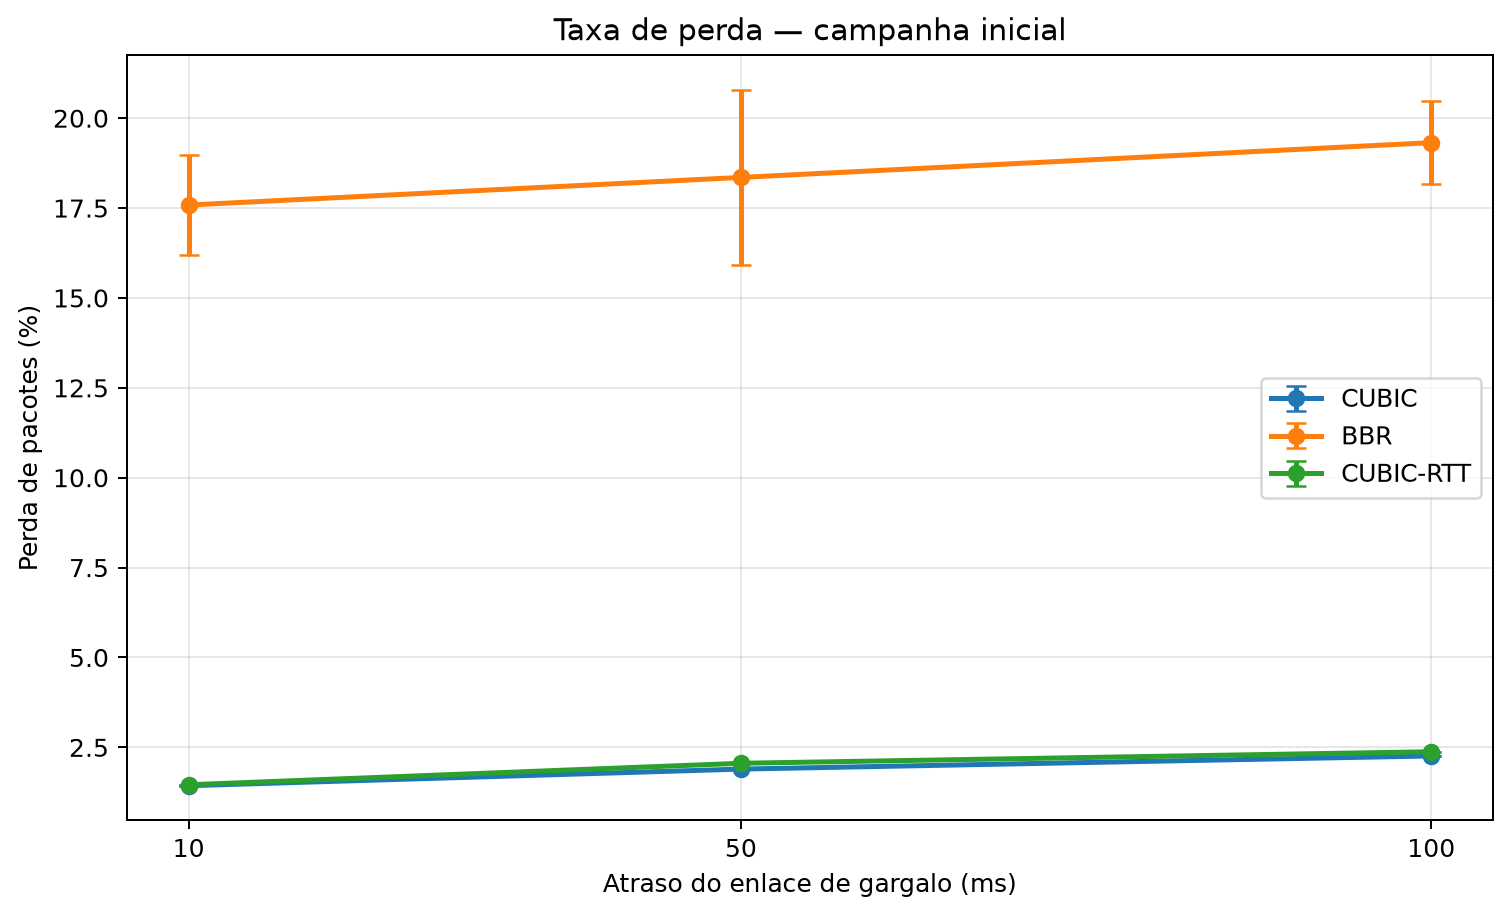
\includegraphics[width=0.88\textwidth]{inicial_packet_loss.png}
\caption{Taxa de perda de pacotes na campanha inicial.}
\label{fig:inicial-perda}
\end{figure}

\subsubsection{Atraso médio e RTT}

O atraso médio unidirecional aumentou à medida que o atraso configurado no gargalo passou de 10 ms para 100 ms. Para o CUBIC, as médias foram 311,71 ms, 409,79 ms e 532,50 ms. Para o CUBIC-RTT, foram 319,91 ms, 419,28 ms e 545,39 ms. Em todos os cenários, portanto, a proposta apresentou atraso médio superior, com diferenças de 8,20 ms, 9,49 ms e 12,89 ms.

Esse resultado é importante porque delimita o alcance da hipótese inicial. A utilização de RTT na adaptação não produziu, nessa campanha, uma redução do atraso médio de entrega. O mecanismo considera o menor RTT observado em relação a uma referência, e não atua diretamente sobre cada aumento instantâneo de atraso provocado pelo enfileiramento.

\begin{figure}[htbp]
\centering
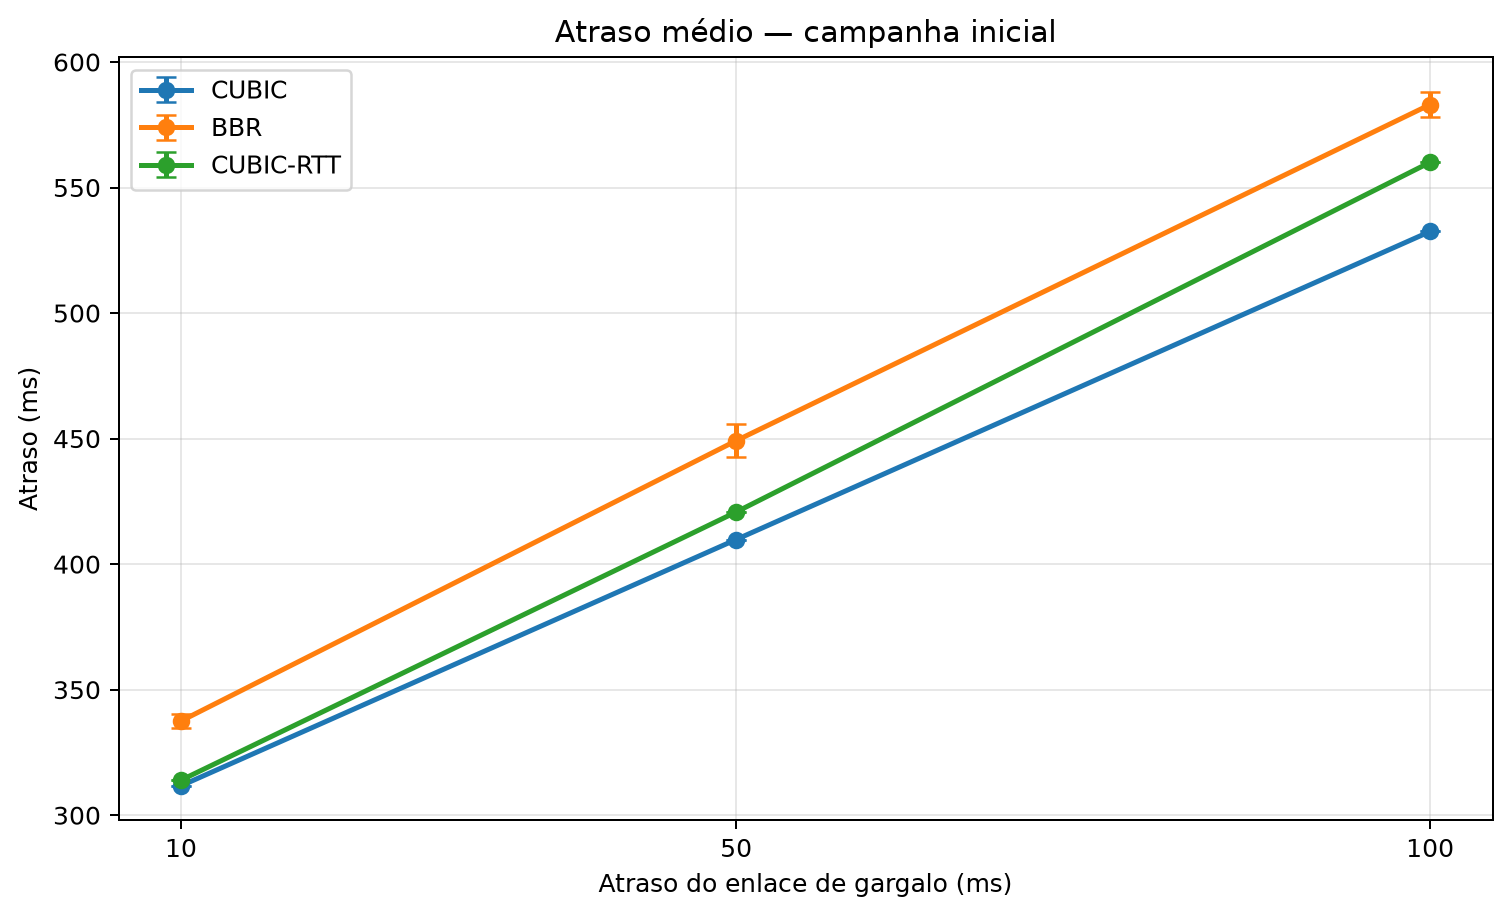
\includegraphics[width=0.88\textwidth]{inicial_delay.png}
\caption{Atraso médio unidirecional na campanha inicial.}
\label{fig:inicial-atraso}
\end{figure}

O gráfico de RTT médio complementa essa leitura, pois apresenta a medida de ida e volta observada pela conexão, distinta do atraso unidirecional do FlowMonitor. As duas métricas não são intercambiáveis: a primeira alimenta a lógica adaptativa do CUBIC-RTT, enquanto a segunda descreve o tempo de entrega dos pacotes em um sentido.

\begin{figure}[htbp]
\centering
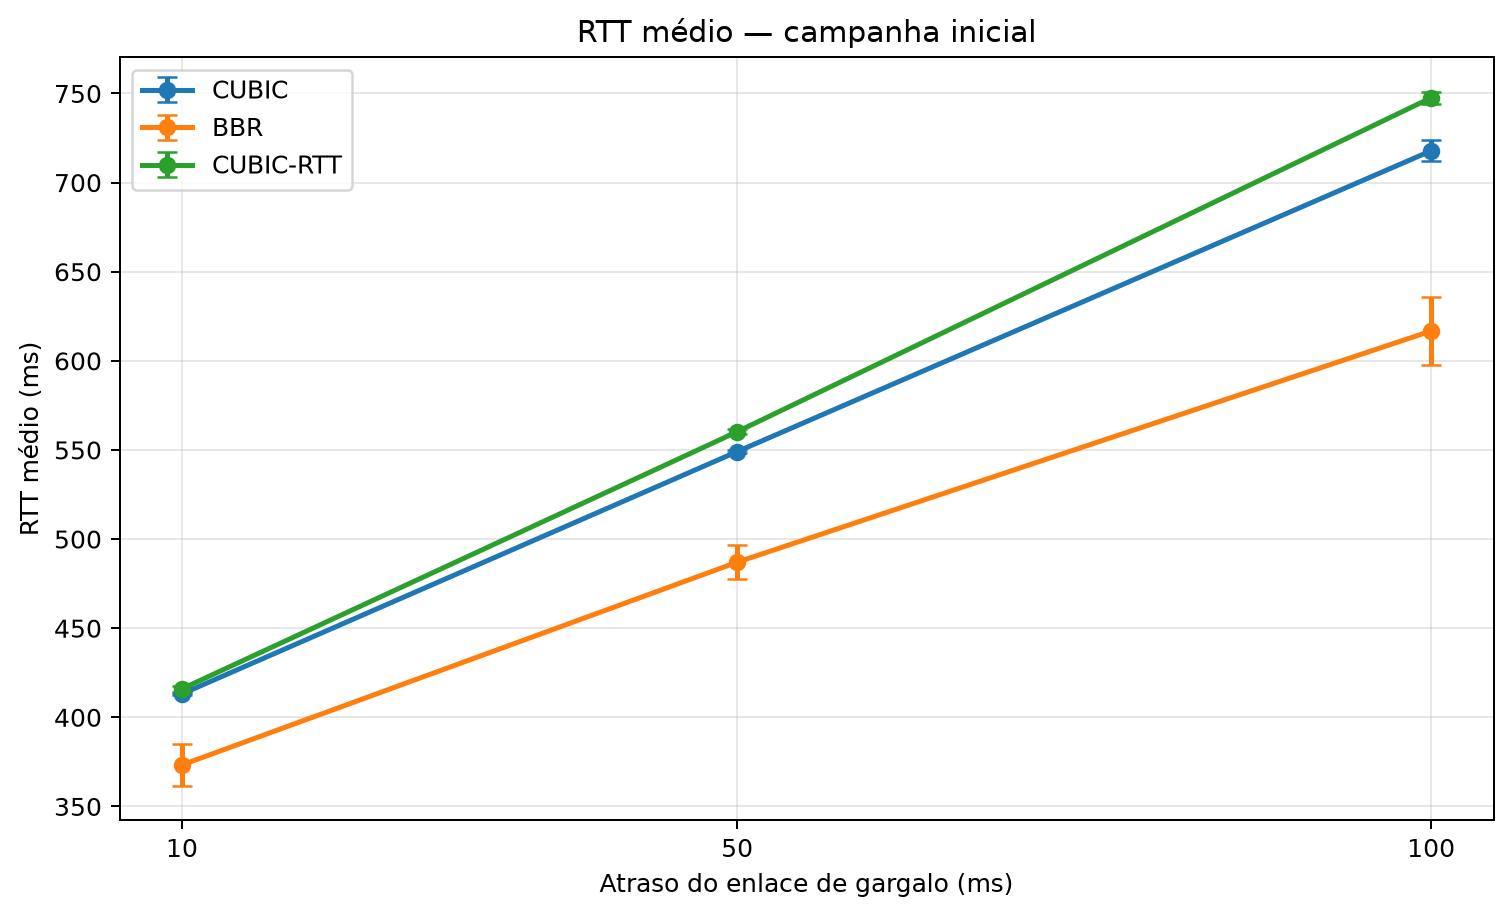
\includegraphics[width=0.88\textwidth]{inicial_rtt.png}
\caption{RTT médio observado na campanha inicial.}
\label{fig:inicial-rtt}
\end{figure}

\subsubsection{Jitter}

O resultado mais favorável ao CUBIC-RTT na comparação inicial foi o jitter. A proposta registrou 1,610 ms, 1,595 ms e 1,659 ms, enquanto o CUBIC apresentou 1,632 ms, 1,650 ms e 1,718 ms. As reduções foram de aproximadamente 1,3\%, 3,3\% e 3,4\%.

As diferenças absolutas são moderadas, mas mantêm o mesmo sentido nos três atrasos avaliados. O BBR apresentou jitter ainda menor, entre 1,060 ms e 1,190 ms, mas esse resultado ocorreu junto de perdas de pacotes muito superiores às observadas nos dois algoritmos CUBIC.

\begin{figure}[htbp]
\centering
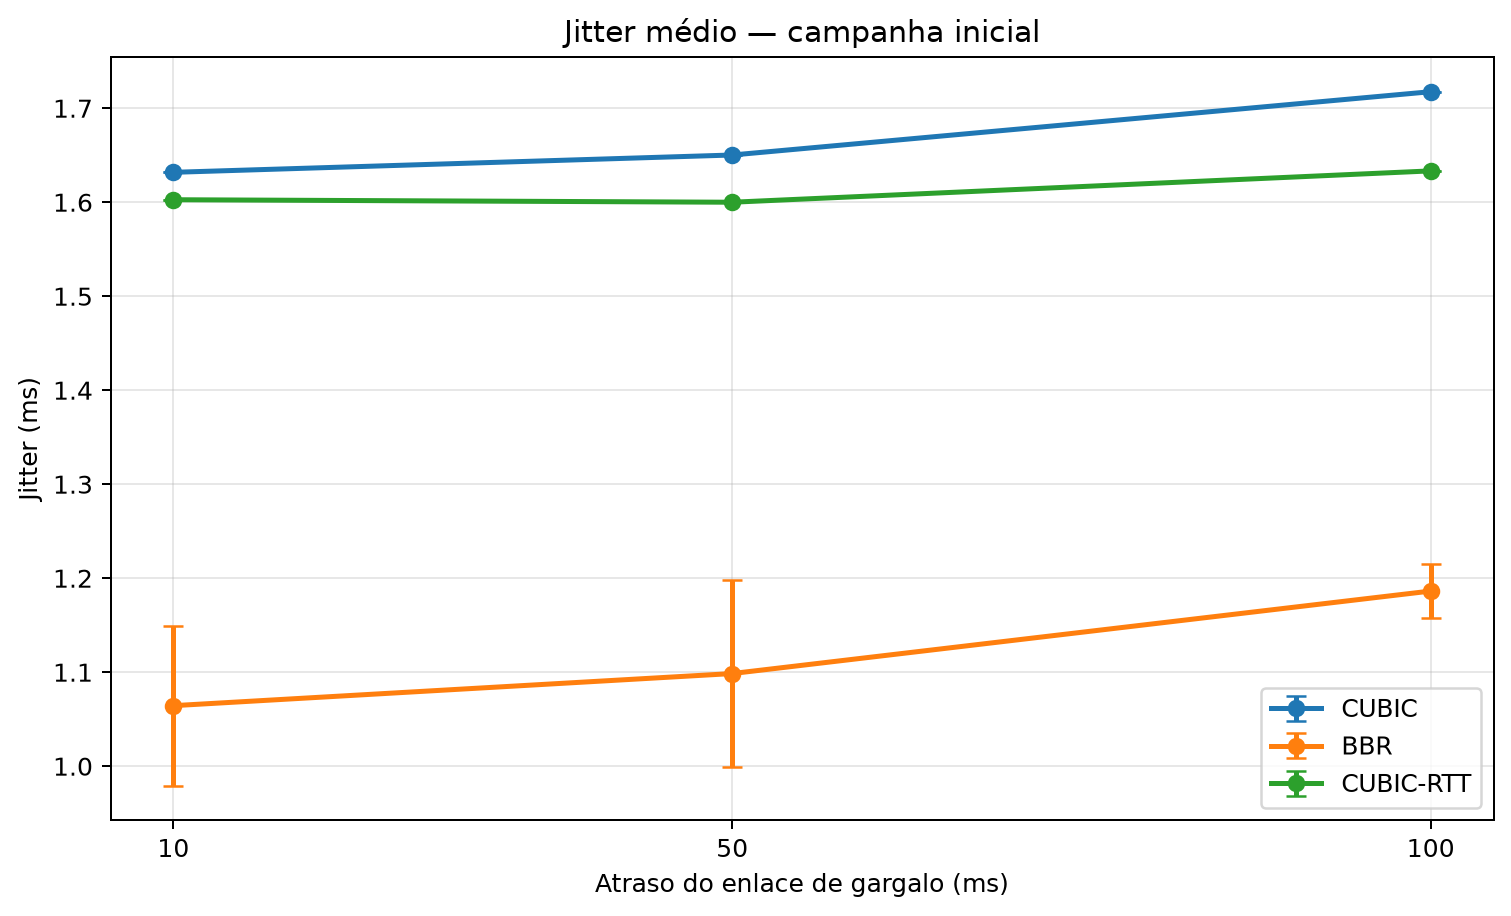
\includegraphics[width=0.88\textwidth]{inicial_jitter.png}
\caption{Jitter médio na campanha inicial.}
\label{fig:inicial-jitter}
\end{figure}

Em resumo, os resultados iniciais indicam que a adaptação pode alterar a regularidade temporal da entrega sem reduzir a vazão agregada. Essa mudança, porém, não veio acompanhada de menor atraso ou menor perda de forma consistente. A primeira campanha sustenta a hipótese de que informações de RTT influenciam o comportamento do CUBIC, mas não demonstra melhoria global em todas as métricas.

\subsection{Campanha de Robustez e Variação de Parâmetros}

A campanha de robustez reuniu 675 simulações, distribuídas em três cenários de rede, quinze configurações de algoritmo e parâmetros, três atrasos de gargalo e cinco repetições. Foram avaliados o CUBIC original, o BBR e treze configurações do CUBIC-RTT, incluindo a configuração de referência ($\alpha=0{,}25$ e $\gamma=0{,}05$).

Os mapas de calor preservados no projeto permitem examinar em detalhe os cenários \texttt{bw1\_f4} e \texttt{bw2\_f8}. O cenário \texttt{access100} também integrou a matriz de execução e a auditoria estrutural, mas não possui, no conjunto de figuras desta versão, mapas equivalentes que permitam uma discussão numérica com o mesmo nível de detalhe. Por isso, a comparação quantitativa a seguir concentra-se nos dois cenários com resultados gráficos disponíveis.

\subsubsection{Cenário bw1\_f4: gargalo de 1 Mbps e quatro fluxos}

Nesse cenário, a vazão permaneceu próxima de 0,99 Mbps para o CUBIC e para todas as configurações CUBIC-RTT, independentemente do atraso do gargalo. Isso indica que a capacidade disponível foi praticamente toda utilizada e que a variação de $\alpha$ e $\gamma$ não produziu diferenças relevantes na vazão agregada.

As diferenças aparecem com maior clareza nas demais métricas. Com 100 ms de atraso, o CUBIC apresentou perda de 3,52\%, atraso médio de 652,12 ms, jitter de 3,57 ms e índice de Jain de 0,97. A configuração de referência do CUBIC-RTT apresentou, no mesmo cenário, perda de 4,11\%, atraso de 661,68 ms, jitter de 3,53 ms e índice de Jain de 0,99. Houve, então, pequena redução de jitter e melhor distribuição entre os fluxos, mas com aumento da perda e do atraso médio.

A variação dos coeficientes mostra que não existe uma combinação que minimize simultaneamente todas as métricas. Por exemplo, com 100 ms, a configuração $\alpha=0{,}50$ e $\gamma=0{,}025$ apresentou atraso médio de 633,86 ms, abaixo dos 652,12 ms do CUBIC. Entretanto, sua perda foi de 4,75\%, superior aos 3,52\% do algoritmo original, e o jitter chegou a 3,69 ms. Já a configuração $\alpha=0{,}10$ e $\gamma=0$ obteve atraso de 641,33 ms e perda de 3,83\%, combinando menor atraso que o CUBIC com perda um pouco maior.

O BBR manteve vazão próxima de 0,97 Mbps, mas apresentou perdas de 4,30\%, 17,70\% e 18,57\% nos três atrasos. Seu índice de Jain caiu para 0,65 em 50 ms e 0,82 em 100 ms. Novamente, esses números caracterizam o cenário simulado, não uma propriedade universal do BBR.

\subsubsection{Cenário bw2\_f8: gargalo de 2 Mbps e oito fluxos}

Com oito fluxos concorrentes e gargalo de 2 Mbps, a vazão também permaneceu próxima da capacidade disponível. CUBIC e CUBIC-RTT registraram aproximadamente 1,98 Mbps em 10 ms e 1,97 Mbps em 50 ms e 100 ms. A mudança dos coeficientes teve pouco efeito sobre essa métrica agregada.

A diferença entre as configurações voltou a aparecer no atraso, no jitter, na perda e na justiça. Com 100 ms, o CUBIC apresentou atraso médio de 548,06 ms, jitter de 2,19 ms, perda de 2,76\% e índice de Jain de 0,96. A configuração de referência do CUBIC-RTT apresentou atraso de 556,43 ms, jitter de 2,18 ms, perda de 3,21\% e índice de Jain de 0,94. Nesse caso, a pequena redução de jitter veio acompanhada de aumento do atraso e da perda e de uma distribuição um pouco menos equilibrada.

Algumas combinações produziram compromissos diferentes. A configuração $\alpha=0{,}10$ e $\gamma=0{,}10$, por exemplo, reduziu o jitter para 1,90 ms, 1,87 ms e 1,93 ms nos três atrasos, abaixo dos valores do CUBIC. Em contrapartida, com 100 ms, seu atraso médio foi de 578,82 ms e a perda foi de 3,11\%, ambos superiores aos do algoritmo original. Por outro lado, configurações com $\gamma=0$ chegaram a apresentar atraso médio menor em 100 ms, mas sem manter a mesma vantagem em jitter e perda.

O BBR apresentou perdas entre 20,15\% e 21,48\% e índices de Jain entre 0,46 e 0,74. Embora sua vazão tenha permanecido próxima de 1,93--1,95 Mbps, a distribuição entre os oito fluxos foi consideravelmente menos equilibrada nesse cenário específico.

\subsubsection{Influência dos coeficientes \texorpdfstring{$\alpha$ e $\gamma$}{alpha e gamma}}

Os mapas de calor mostram que a influência dos coeficientes depende do cenário e da métrica observada. O coeficiente $\alpha$ altera a intensidade da adaptação do fator cúbico $C$, afetando o crescimento da janela. O coeficiente $\gamma$ modula a alteração de $\beta$ após a perda. Como os dois mecanismos atuam em momentos diferentes do controle de congestionamento, seus efeitos não precisam aparecer simultaneamente nem na mesma direção em todas as métricas.

De forma geral, a vazão agregada permaneceu próxima ao limite do gargalo em quase todas as configurações. Isso significa que a comparação entre parâmetros é mais informativa quando se observam atraso, jitter, perda e justiça. Em algumas condições, determinadas combinações reduziram o atraso ou o jitter, mas aumentaram a perda de pacotes; em outras, melhoraram o índice de Jain sem oferecer vantagem de vazão. A configuração de referência, portanto, deve ser entendida como um ponto de partida para a avaliação, e não como uma escolha ótima para todos os cenários.

A campanha de robustez reforça a conclusão da comparação inicial: a adaptação baseada em RTT modifica o comportamento do CUBIC e pode favorecer uma métrica em determinadas condições, mas o efeito não é uniforme. Não foi identificada uma combinação de $\alpha$ e $\gamma$ que dominasse o CUBIC original em vazão, atraso, jitter, perda e justiça ao mesmo tempo.

\subsection{Coexistência entre Fluxos CUBIC e CUBIC-RTT}

A campanha de coexistência avalia uma questão diferente das comparações anteriores: não apenas como cada algoritmo se comporta isoladamente, mas como os dois disputam a mesma capacidade de transmissão. Foram utilizados oito fluxos simultâneos, quatro CUBIC e quatro CUBIC-RTT, com a mesma configuração de referência da proposta ($\alpha=0{,}25$ e $\gamma=0{,}05$). Os enlaces de acesso foram distribuídos em pares com atrasos de 10 ms, 30 ms, 60 ms e 90 ms, enquanto o gargalo de 10 Mbps foi avaliado com atrasos de 10 ms, 50 ms e 100 ms.

A Tabela~\ref{tab:coexistencia} apresenta a vazão média por fluxo, o atraso médio, o jitter e a perda de cada grupo. Para cada repetição, foram calculadas as médias dos quatro fluxos pertencentes ao mesmo algoritmo; em seguida, foram calculadas as médias das cinco repetições. A perda foi consolidada pela razão entre pacotes perdidos e pacotes transmitidos.

\begin{table}[htbp]
\centering
\caption{Resultados médios da campanha de coexistência}
\label{tab:coexistencia}
\small
\resizebox{\textwidth}{!}{
\begin{tabular}{c l r r r r}
\toprule
\textbf{Atraso do gargalo} & \textbf{Algoritmo} & \textbf{Vazão por fluxo (Mbps)} & \textbf{Perda (\%)} & \textbf{Atraso médio (ms)} & \textbf{Jitter (ms)} \\
\midrule
10 ms & CUBIC & 1,2492 & 0,2465 & 450,008 & 0,6100 \\
10 ms & CUBIC-RTT & 1,2345 & 0,2416 & 449,700 & 0,6131 \\
\midrule
50 ms & CUBIC & 1,2068 & 0,3229 & 552,776 & 0,6487 \\
50 ms & CUBIC-RTT & 1,2757 & 0,3177 & 552,603 & 0,6380 \\
\midrule
100 ms & CUBIC & 1,1070 & 0,5070 & 678,778 & 0,7060 \\
100 ms & CUBIC-RTT & 1,3746 & 0,4590 & 678,291 & 0,6556 \\
\bottomrule
\end{tabular}}
\end{table}

\subsubsection{Vazão: redistribuição da capacidade entre os algoritmos}

Com atraso de gargalo de 10 ms, a vazão média por fluxo CUBIC foi de 1,2492 Mbps, ligeiramente superior aos 1,2345 Mbps do CUBIC-RTT. A diferença representa aproximadamente 1,2\%. Em 50 ms, a relação se inverteu: o CUBIC-RTT alcançou 1,2757 Mbps por fluxo, contra 1,2068 Mbps do CUBIC, uma vantagem de aproximadamente 5,7\%.

A diferença ficou mais evidente em 100 ms. O CUBIC-RTT atingiu 1,3746 Mbps por fluxo, enquanto o CUBIC caiu para 1,1070 Mbps, o que representa uma vantagem de aproximadamente 24,2\% para a variante adaptativa. Como cada algoritmo possui quatro fluxos, a vazão total da rede permaneceu próxima de 9,93 Mbps nos três cenários. Na prática, o aumento da vazão do CUBIC-RTT não representa um crescimento equivalente da capacidade total utilizada: representa principalmente uma redistribuição da banda em favor dos fluxos que executam a proposta.

A participação do CUBIC-RTT na vazão total passou de aproximadamente 49,7\% em 10 ms para 51,4\% em 50 ms e 55,4\% em 100 ms. Esse resultado é central para a avaliação da hipótese: a adaptação pode manter a utilização do gargalo e, ao mesmo tempo, tornar o CUBIC-RTT mais competitivo que o CUBIC original quando os atrasos aumentam. Isso também significa que a proposta não é neutra em relação a fluxos CUBIC concorrentes.

\begin{figure}[htbp]
\centering
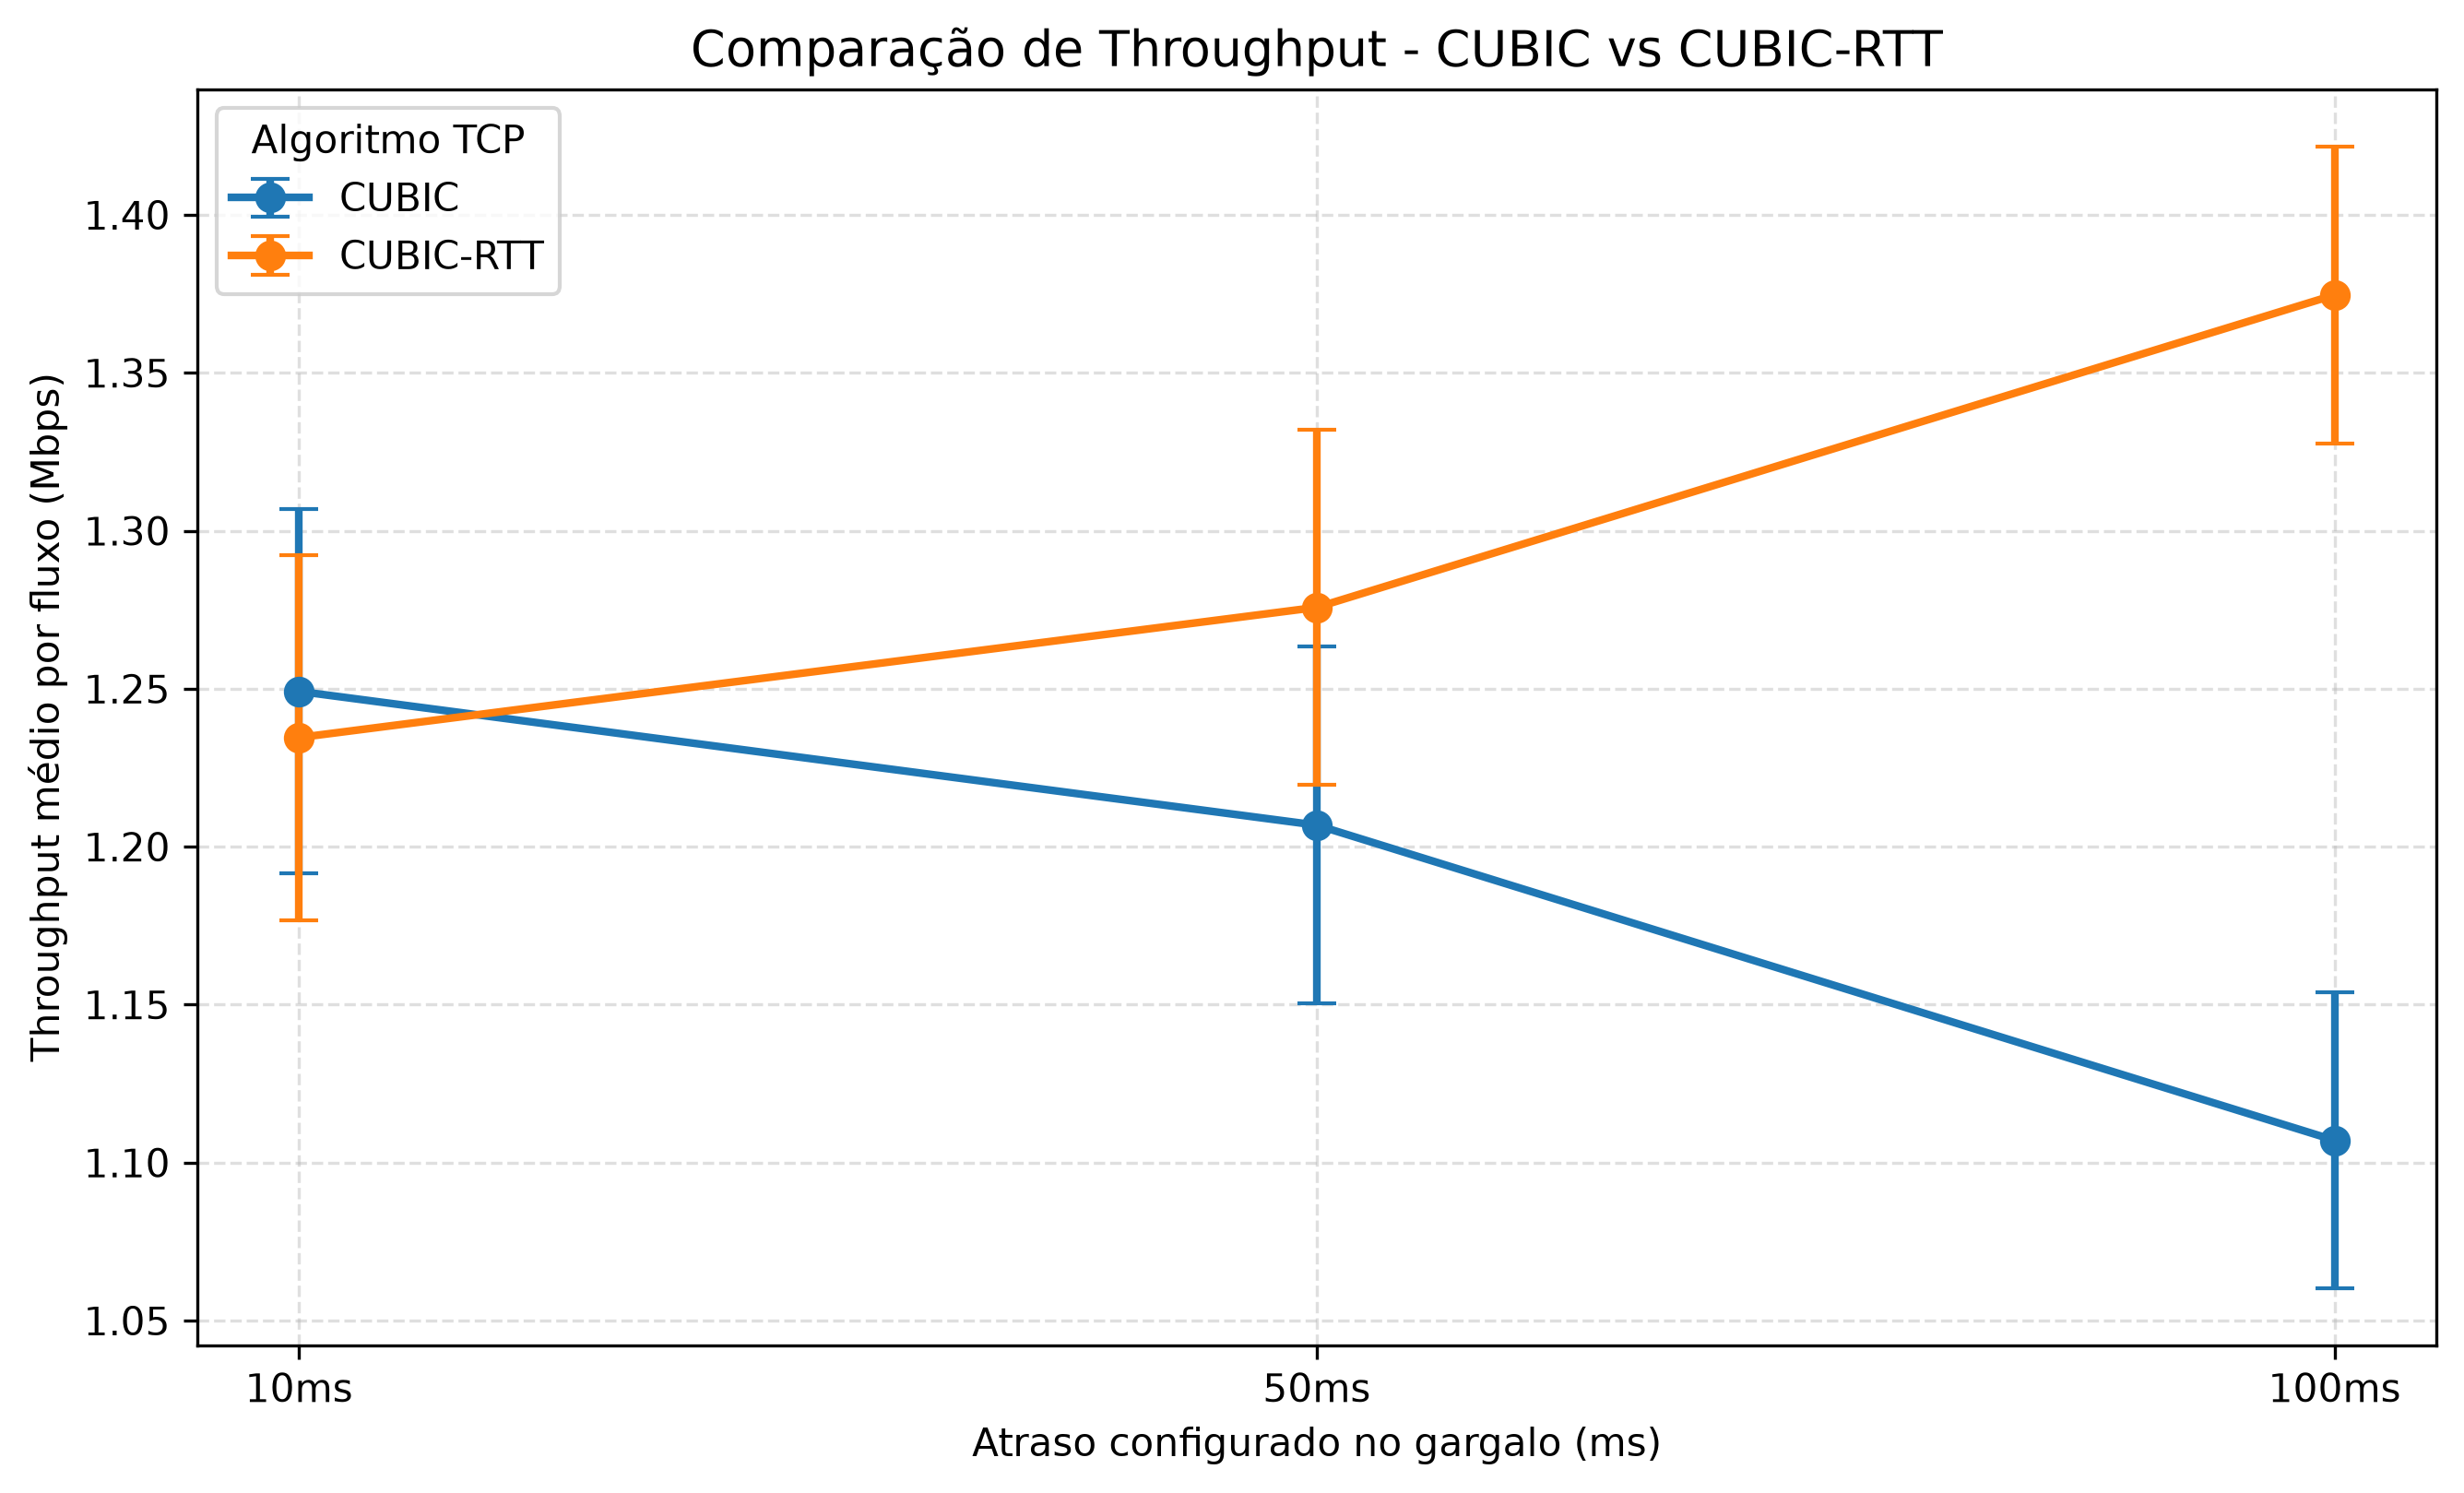
\includegraphics[width=0.90\textwidth]{01_throughput.png}
\caption{Vazão média por fluxo na campanha de coexistência.}
\label{fig:coex-throughput}
\end{figure}

\subsubsection{Atraso médio}

O atraso médio dos dois grupos permaneceu praticamente igual em todos os cenários. Em 10 ms, a diferença foi de aproximadamente 0,31 ms; em 50 ms, 0,17 ms; e em 100 ms, 0,49 ms. Essas diferenças são muito pequenas quando comparadas aos valores absolutos, que cresceram de aproximadamente 450 ms para 678 ms à medida que o atraso do gargalo aumentou.

Na prática, o ganho de vazão do CUBIC-RTT em 50 ms e 100 ms não foi acompanhado por uma redução expressiva do atraso médio. Os dois algoritmos experimentaram condições de atraso muito próximas, embora tenham obtido parcelas diferentes da vazão disponível.

\begin{figure}[htbp]
\centering
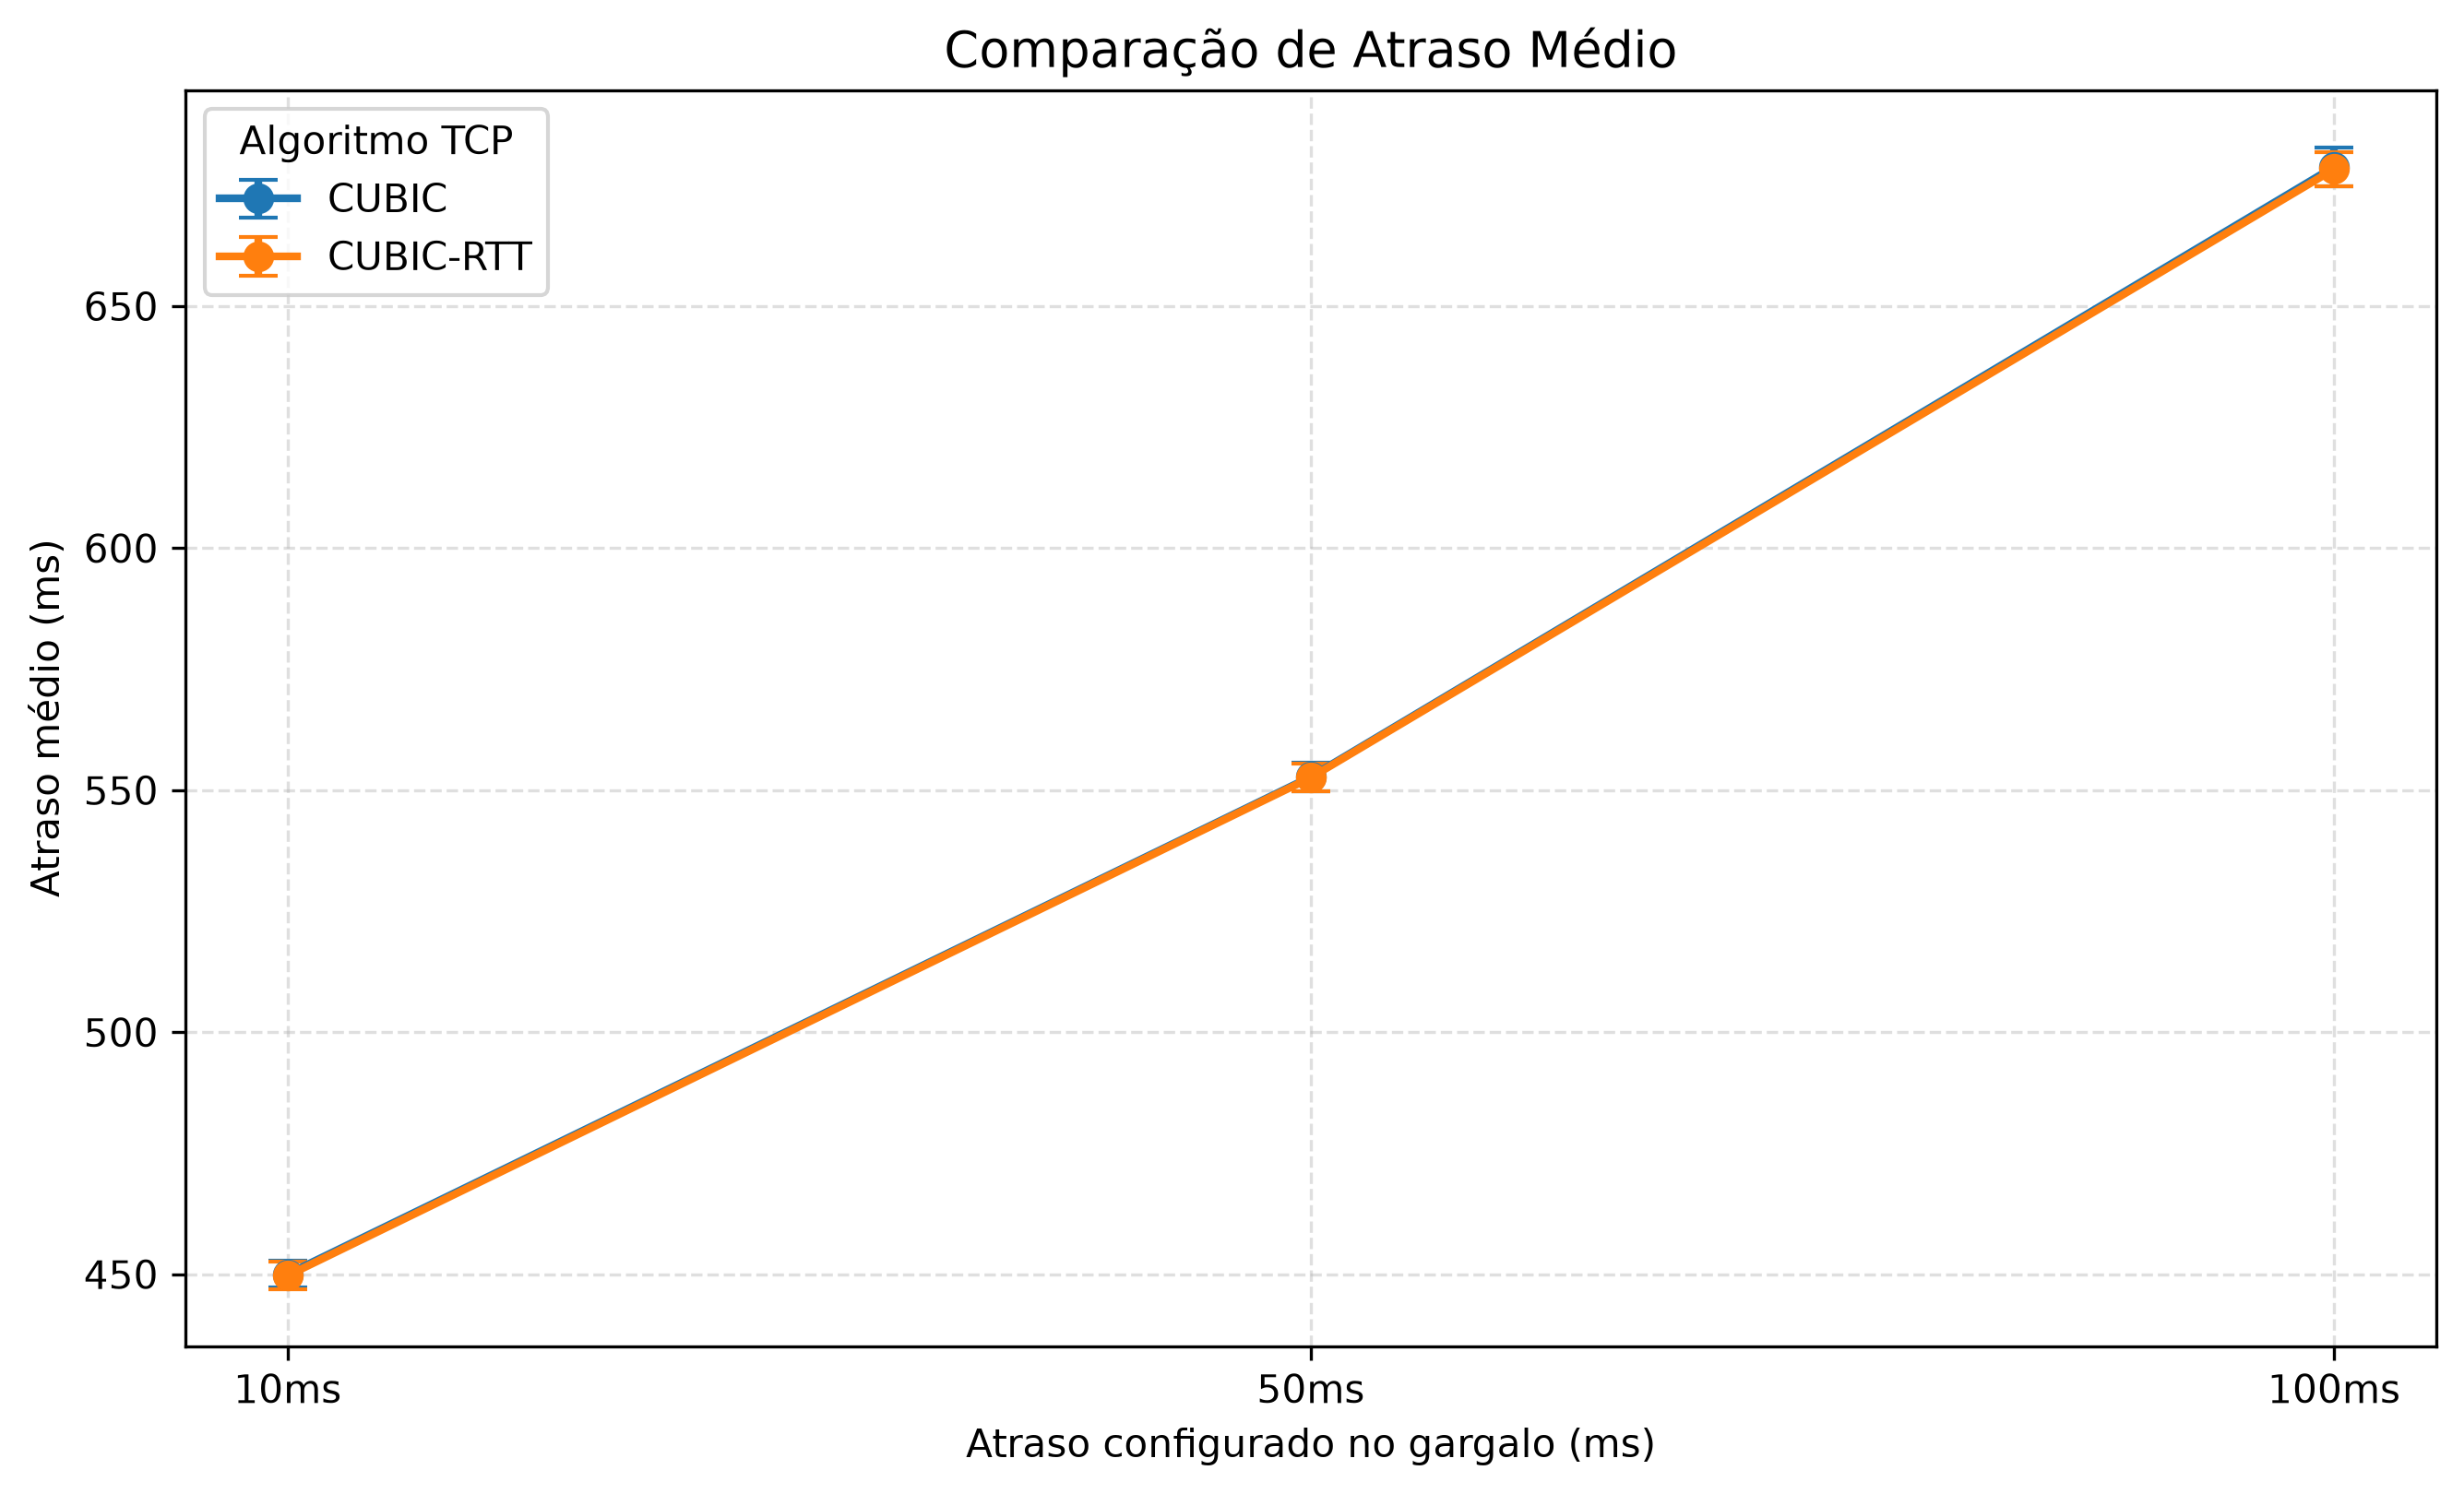
\includegraphics[width=0.90\textwidth]{02_atraso_medio.png}
\caption{Atraso médio dos fluxos na campanha de coexistência.}
\label{fig:coex-atraso}
\end{figure}

\subsubsection{Jitter e perda de pacotes}

No cenário de 10 ms, o jitter dos dois algoritmos foi praticamente igual: 0,6100 ms para CUBIC e 0,6131 ms para CUBIC-RTT. Em 50 ms, o jitter do CUBIC-RTT foi menor, 0,6380 ms contra 0,6487 ms. Em 100 ms, a diferença aumentou: 0,6556 ms para a proposta e 0,7060 ms para o CUBIC, uma redução aproximada de 7,1\%.

A perda de pacotes também foi ligeiramente menor para o CUBIC-RTT nos três atrasos. Em 10 ms, os valores foram 0,2416\% e 0,2465\%; em 50 ms, 0,3177\% e 0,3229\%; e em 100 ms, 0,4590\% e 0,5070\%. A diferença mais perceptível ocorreu no maior atraso, em que a perda do CUBIC-RTT ficou aproximadamente 9,5\% abaixo da observada no CUBIC.

\begin{figure}[htbp]
\centering
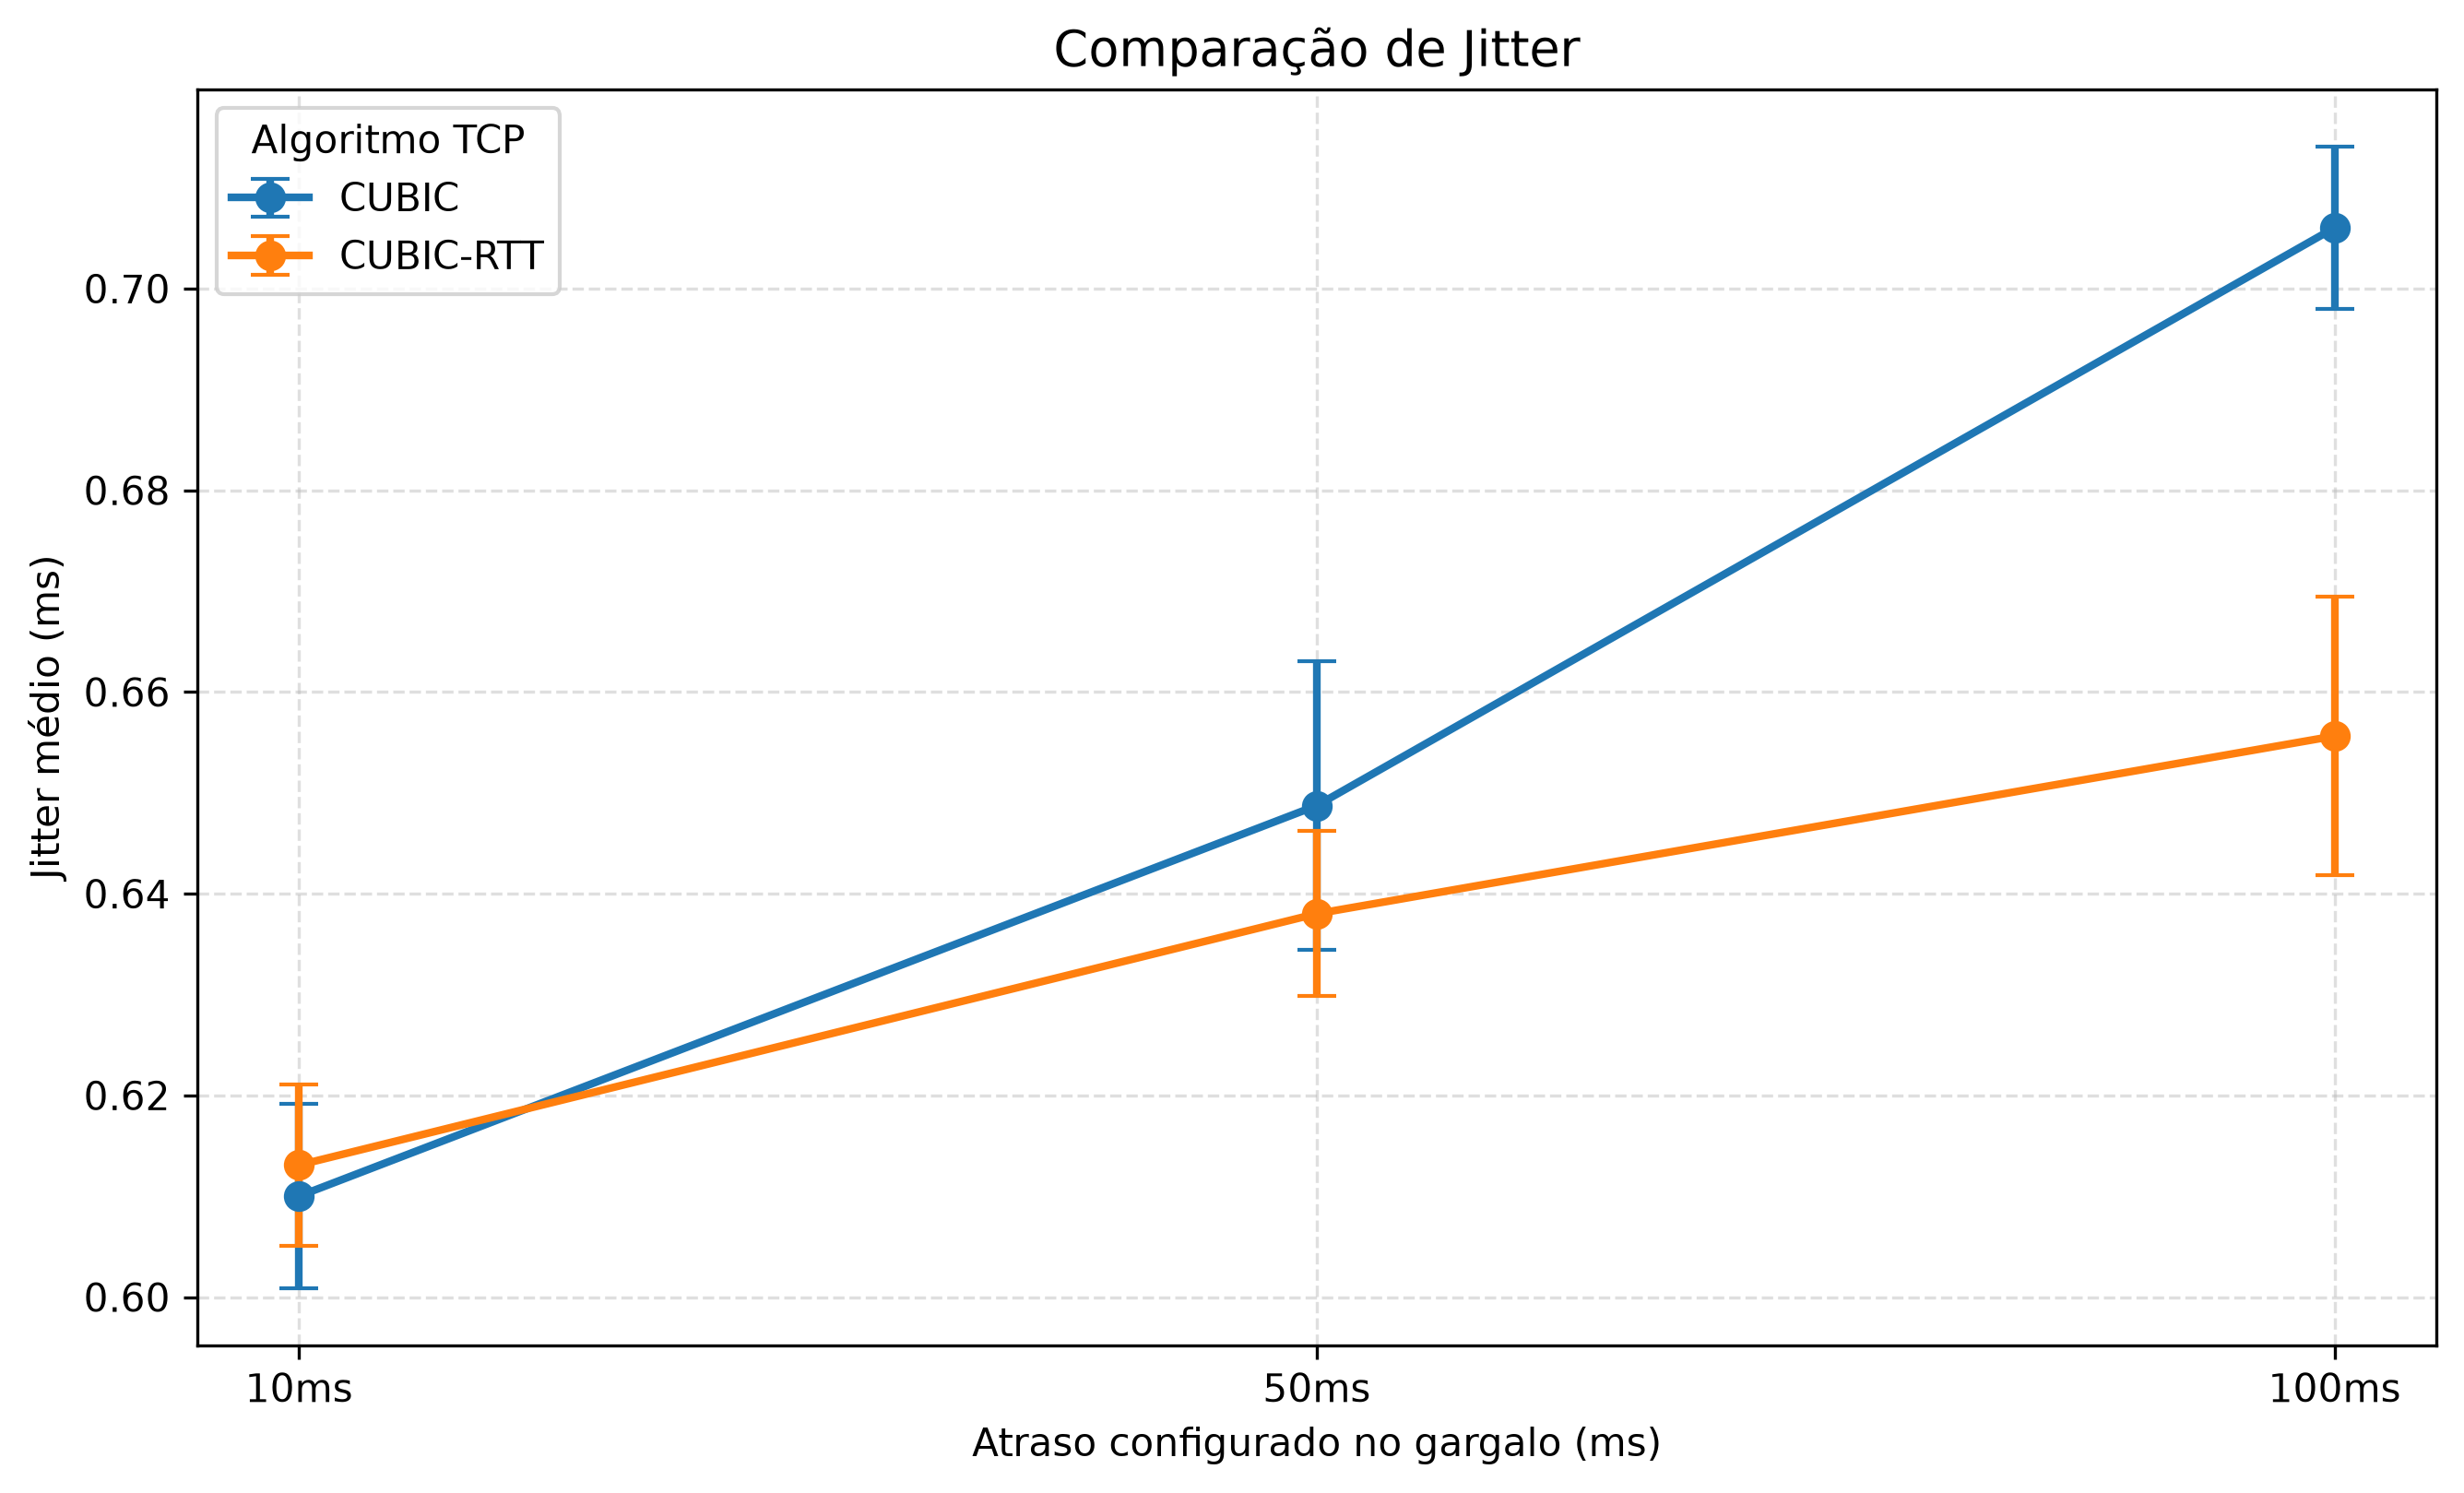
\includegraphics[width=0.90\textwidth]{03_jitter.png}
\caption{Jitter médio na campanha de coexistência.}
\label{fig:coex-jitter}
\end{figure}

\begin{figure}[htbp]
\centering
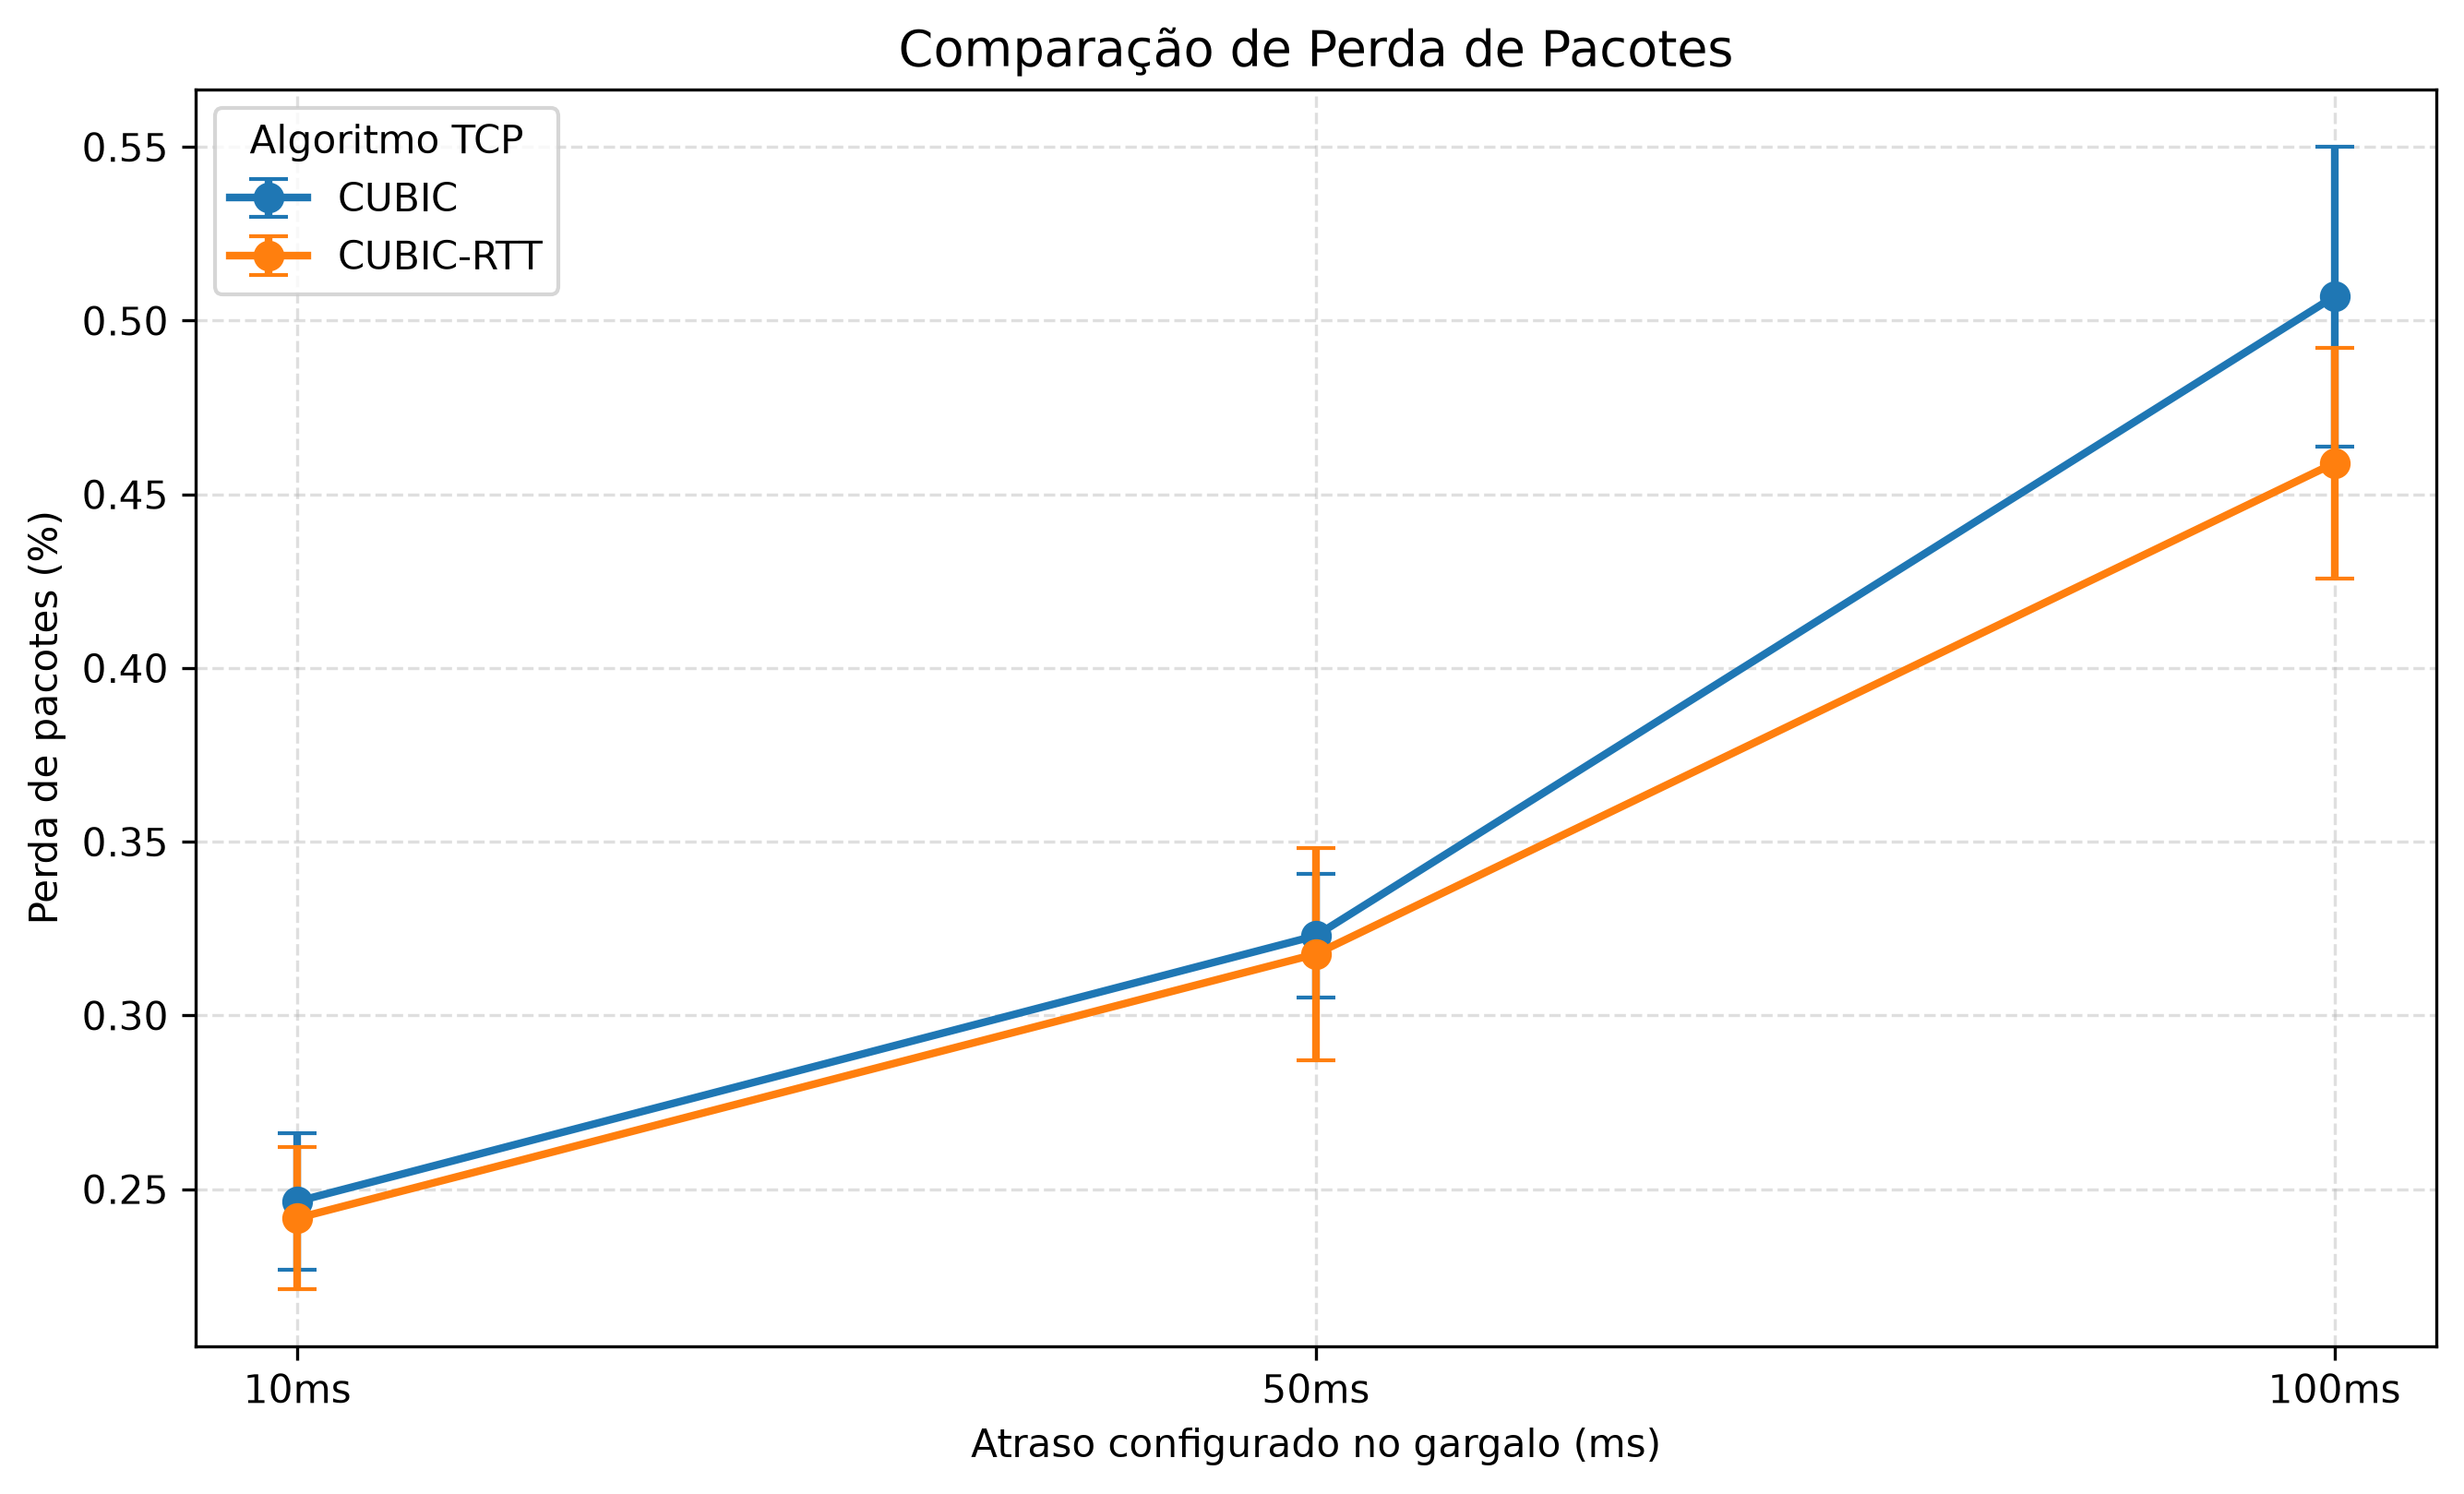
\includegraphics[width=0.90\textwidth]{04_packet_loss.png}
\caption{Taxa de perda de pacotes na campanha de coexistência.}
\label{fig:coex-perda}
\end{figure}

\subsubsection{Interpretação da coexistência}

A campanha mostra que o CUBIC-RTT consegue coexistir com o CUBIC sem derrubar a vazão total da rede e sem diferença expressiva no atraso médio. Coexistir, no entanto, não significa dividir os recursos igualmente: à medida que o atraso do gargalo aumentou, os fluxos CUBIC-RTT ficaram com uma fatia cada vez maior da capacidade, enquanto a vazão média dos fluxos CUBIC diminuiu.

Esse resultado sugere que a adaptação baseada em RTT dá à variante uma vantagem competitiva em cenários de maior atraso. A vantagem veio acompanhada de jitter e perda ligeiramente menores, mas não de uma redução significativa do atraso médio. Por isso, a proposta não deve ser descrita como uma simples melhoria de desempenho: ela muda a relação competitiva entre os algoritmos e pode favorecer quem a utiliza.

O ponto é relevante para a hipótese do trabalho. A informação de RTT mostrou-se útil para modificar a dinâmica do CUBIC, mas o experimento também deixa claro que uma adaptação vantajosa para os fluxos modificados pode reduzir a parcela de banda dos fluxos que continuam usando o algoritmo original. A avaliação da justiça entre algoritmos precisa, portanto, caminhar junto com a avaliação do desempenho individual.

\subsection{Análise das Variáveis Internas do TCP}

Os rastros de CWND, SSThresh, RTT, RTO e quantidade de dados em trânsito foram utilizados para observar a dinâmica das conexões ao longo das simulações. A auditoria estrutural confirmou 3.780 arquivos de CWND e 3.780 de SSThresh nas duas primeiras campanhas, sem pares ausentes, erros ou avisos.

Os gráficos temporais preservados para a campanha de coexistência mostram a evolução da janela de congestionamento e do RTT dos oito fluxos nos três atrasos de gargalo. As curvas apresentam fases iniciais de crescimento, seguidas de oscilações associadas à operação do controle de congestionamento. Com o aumento do atraso, a escala temporal do RTT se desloca para valores maiores, enquanto a janela continua apresentando variações ao longo da execução.

Esses rastros ajudam a interpretar as métricas agregadas, mas não devem ser usados isoladamente para afirmar que um algoritmo é melhor. Sua principal utilidade é permitir relacionar a evolução da janela e do RTT com as diferenças de vazão, jitter e perda observadas no FlowMonitor. Os gráficos representativos são reunidos no Apêndice~\ref{ap:traces}.

\subsection{Discussão Geral}

As três campanhas mostram aspectos complementares da proposta. Na comparação inicial, o CUBIC-RTT manteve a vazão agregada próxima à do CUBIC e reduziu moderadamente o jitter, mas apresentou atraso médio maior e perda ligeiramente superior nos cenários de maior atraso. Na campanha de robustez, a vazão permaneceu próxima da capacidade do gargalo, enquanto as demais métricas variaram de acordo com o cenário e com os valores de $\alpha$ e $\gamma$. Não houve uma configuração que apresentasse o melhor resultado em todas as métricas.

A campanha de coexistência acrescentou um resultado importante: quando CUBIC e CUBIC-RTT compartilham o mesmo gargalo, a variante adaptativa pode obter uma parcela maior da vazão, especialmente quando o atraso do gargalo aumenta. Esse ganho não elevou a vazão total da rede, que permaneceu próxima de 10 Mbps; ele alterou a distribuição da capacidade entre os grupos de fluxos.

Em relação à hipótese de partida, os experimentos sustentam que informações de RTT podem ser incorporadas à estrutura do CUBIC e modificar seu comportamento. Já a expectativa de que essa alteração produza, em qualquer cenário, menor atraso, maior justiça e manutenção integral do desempenho dos fluxos concorrentes não foi confirmada. O resultado mais adequado é considerar o CUBIC-RTT uma variante experimental com efeitos dependentes do cenário e com um compromisso claro entre regularidade, perda e competitividade.

\section{CONSIDERAÇÕES FINAIS}

Este trabalho investigou o comportamento dos algoritmos TCP CUBIC e TCP BBR e desenvolveu uma variante do CUBIC denominada TCP CUBIC-RTT. A proposta foi implementada no simulador \texttt{ns-3} e preservou a estrutura geral do algoritmo original, incorporando informações do menor RTT observado para adaptar o fator de crescimento cúbico $C$ e o fator de redução multiplicativa $\beta$. Os coeficientes $\alpha$ e $\gamma$ controlam a intensidade dessas alterações.

A implementação foi organizada entre o modelo do protocolo e o programa experimental. Foram instrumentados rastros de janela de congestionamento, limiar de congestionamento, RTT, RTO e dados em trânsito, além da coleta das métricas de fluxo pelo FlowMonitor. Durante o desenvolvimento, foi necessário corrigir a topologia para utilizar um gargalo realmente compartilhado, ajustar o caminho de conexão de um callback de rastreamento e filtrar os fluxos reversos de ACK no processamento dos resultados. Essas decisões foram importantes para que a avaliação representasse a disputa pelo enlace e para evitar distorções na consolidação das métricas.

A avaliação reuniu três campanhas, totalizando 735 simulações: a comparação inicial entre CUBIC, BBR e CUBIC-RTT em três atrasos de gargalo, a campanha de robustez, que ampliou os cenários e variou os coeficientes $\alpha$ e $\gamma$, e a campanha de coexistência, que colocou quatro fluxos de cada variante em competição direta pelo mesmo gargalo.

Na comparação inicial, CUBIC e CUBIC-RTT mantiveram vazão agregada praticamente equivalente, e a proposta teve jitter menor nos três atrasos, ao custo de atraso médio maior e, nos cenários de 50 ms e 100 ms, perda também maior. A campanha de robustez confirmou que o efeito da adaptação depende da condição de rede e da combinação dos coeficientes: nenhuma combinação de $\alpha$ e $\gamma$ dominou o CUBIC original em todos os critérios.

A campanha de coexistência revelou um efeito que não apareceria em execuções separadas de cada algoritmo. Com o aumento do atraso do gargalo, a vazão média por fluxo do CUBIC-RTT passou de 1,2345 Mbps em 10 ms para 1,3746 Mbps em 100 ms, enquanto a do CUBIC caiu de 1,2492 Mbps para 1,1070 Mbps, com a vazão total da rede estável em torno de 9,93 Mbps. A vantagem da variante adaptativa foi, portanto, uma redistribuição da capacidade em seu favor, e não um aumento da capacidade utilizada.

Voltando à pergunta que motivou o trabalho, a resposta tem duas partes. Primeiro, foi possível incorporar informações de RTT à estrutura do CUBIC sem trocar sua função cúbica por outro modelo de controle, e essa incorporação mudou o comportamento observado nas simulações. Segundo, não se confirmou que a mudança melhore ao mesmo tempo vazão, atraso, perda e justiça em todas as condições. A campanha de coexistência foi a mais reveladora nesse ponto: uma variante pode ganhar vantagem competitiva sobre fluxos do algoritmo original mesmo quando a utilização total do gargalo praticamente não muda.

A principal contribuição do trabalho é, portanto, a implementação e a avaliação experimental de uma adaptação do CUBIC baseada em RTT, acompanhada da identificação de seus benefícios e de seus limites. Os resultados não sustentam afirmar que o CUBIC-RTT seja universalmente superior ao CUBIC ou ao BBR. Sustentam, porém, que a informação de RTT é um sinal relevante para modificar a dinâmica do algoritmo e que sua utilização precisa ser avaliada também sob competição com fluxos não modificados.

Como trabalhos futuros, recomenda-se aprofundar a análise do cenário \texttt{access100}, ampliar a avaliação de justiça na coexistência e testar a proposta em outras combinações de capacidade, atraso, quantidade de fluxos e disciplinas de fila. Também é relevante investigar mecanismos que utilizem variações recentes do RTT, em vez de depender apenas do menor valor observado. Durante o desenvolvimento foi considerada uma alternativa baseada na variação relativa do RTT suavizada por uma média móvel exponencial (EWMA), aplicada ao fator $C$. Essa alternativa não integra os resultados apresentados e deve ser tratada como uma hipótese para experimentos posteriores. Por fim, a execução em ambiente real e a avaliação de interações com outros algoritmos de controle de congestionamento poderão ampliar a validade externa dos resultados obtidos no simulador.

\appendix

\section{Mapas de Calor da Campanha de Robustez}
\label{ap:robustez}

Os mapas a seguir apresentam, para cada configuração de algoritmo e parâmetros, os valores consolidados nos atrasos de gargalo de 10 ms, 50 ms e 100 ms. As linhas identificam o algoritmo e, no caso do CUBIC-RTT, os valores de $\alpha$ e $\gamma$.

\subsection{Cenário bw1\_f4}

\begin{figure}[p]
\centering
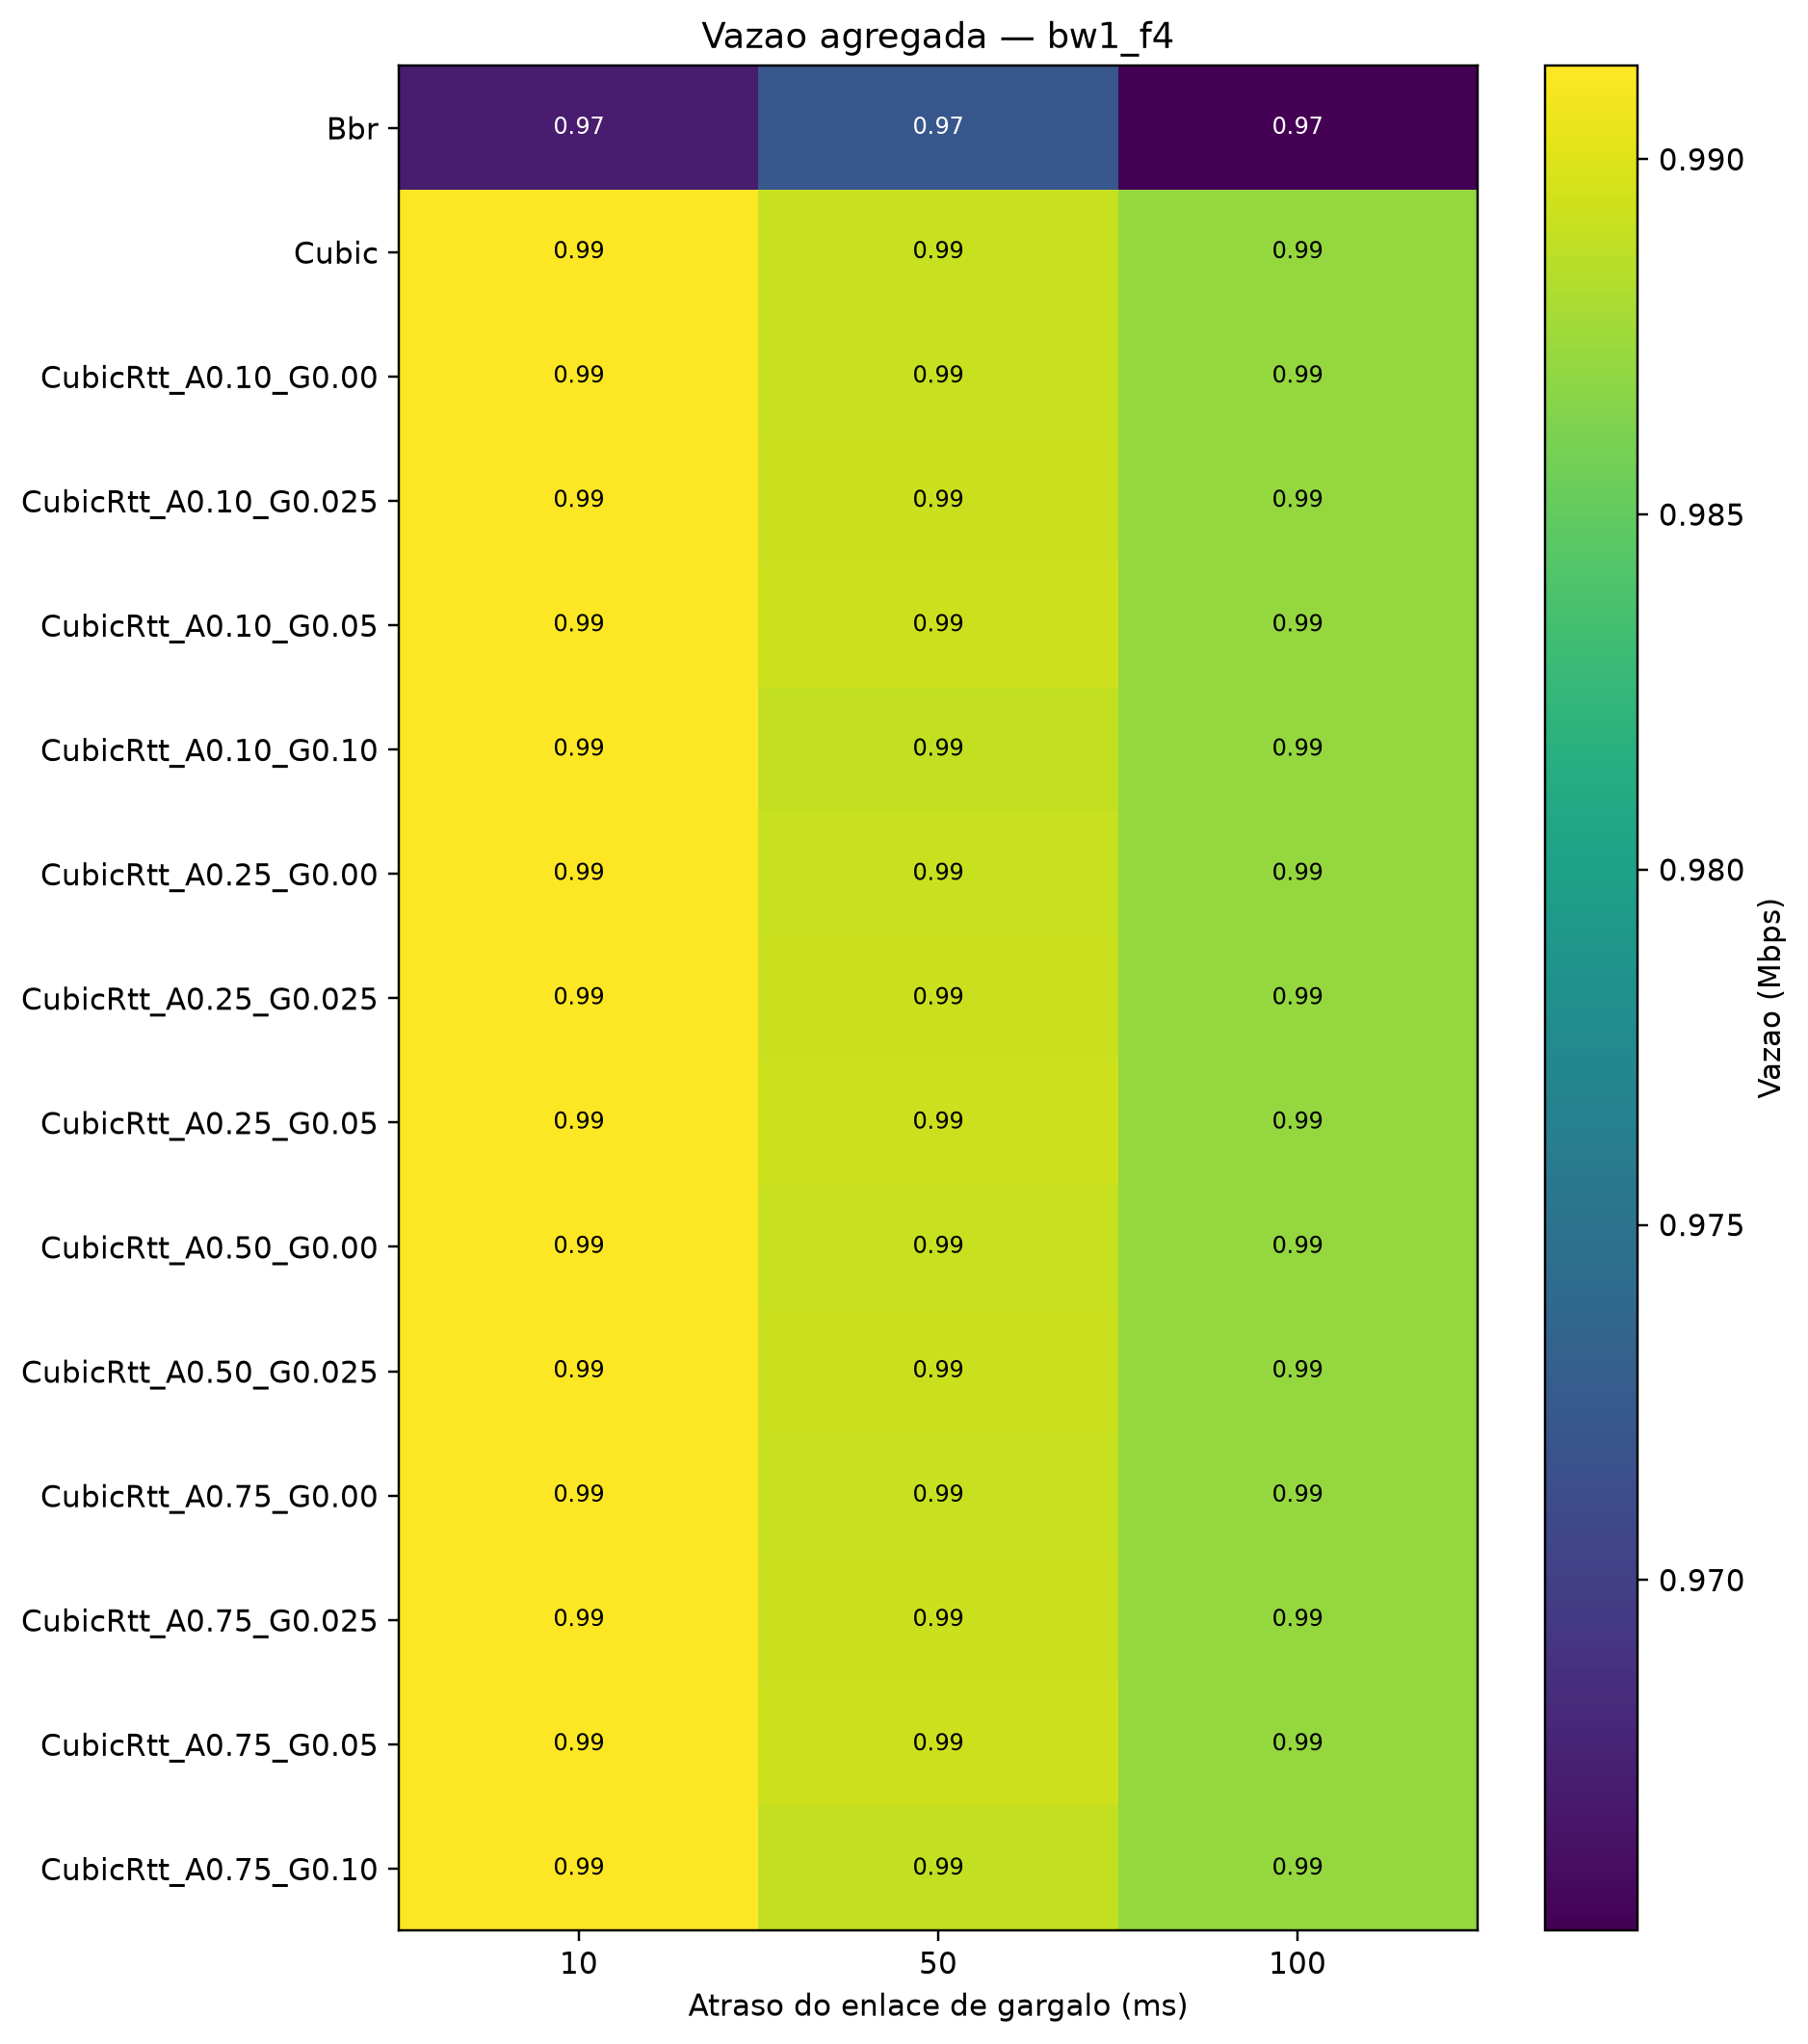
\includegraphics[width=0.88\textwidth]{bw1_f4_throughput_mbps.png}
\caption{Vazão agregada no cenário \texttt{bw1\_f4}.}
\label{fig:bw1-throughput}
\end{figure}

\begin{figure}[p]
\centering
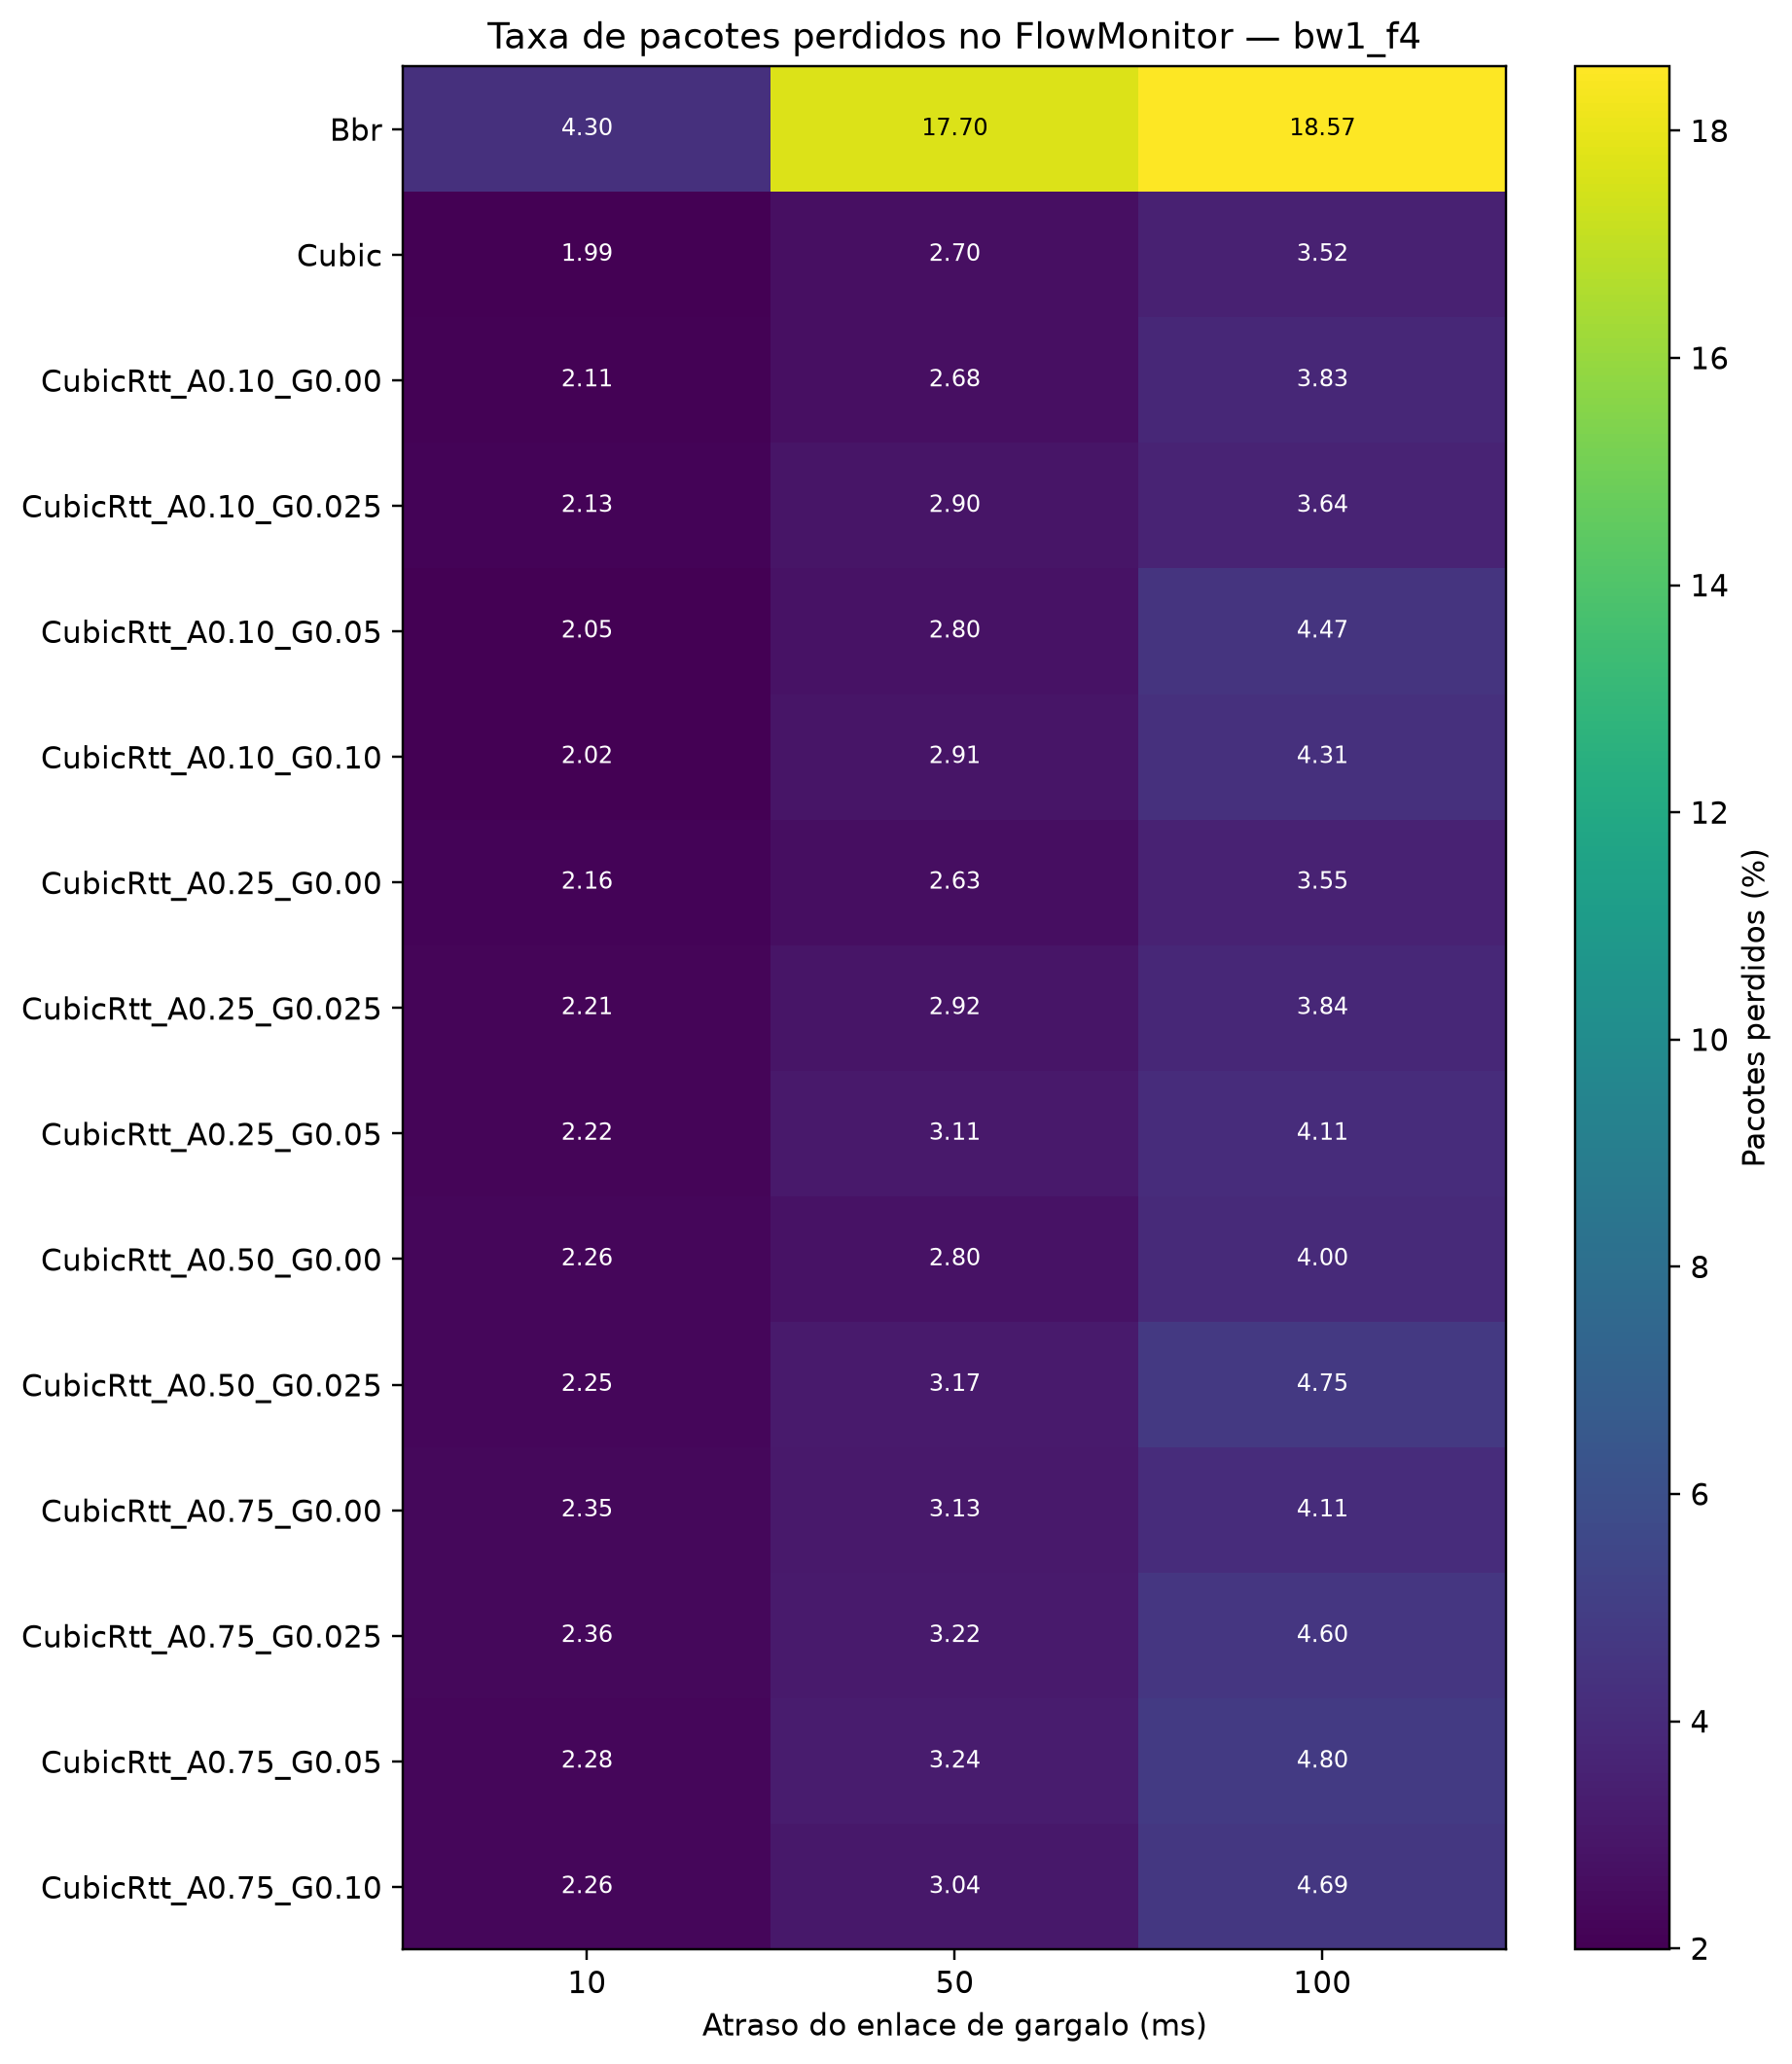
\includegraphics[width=0.88\textwidth]{bw1_f4_loss_rate_pct.png}
\caption{Taxa de perda de pacotes no cenário \texttt{bw1\_f4}.}
\label{fig:bw1-loss}
\end{figure}

\begin{figure}[p]
\centering
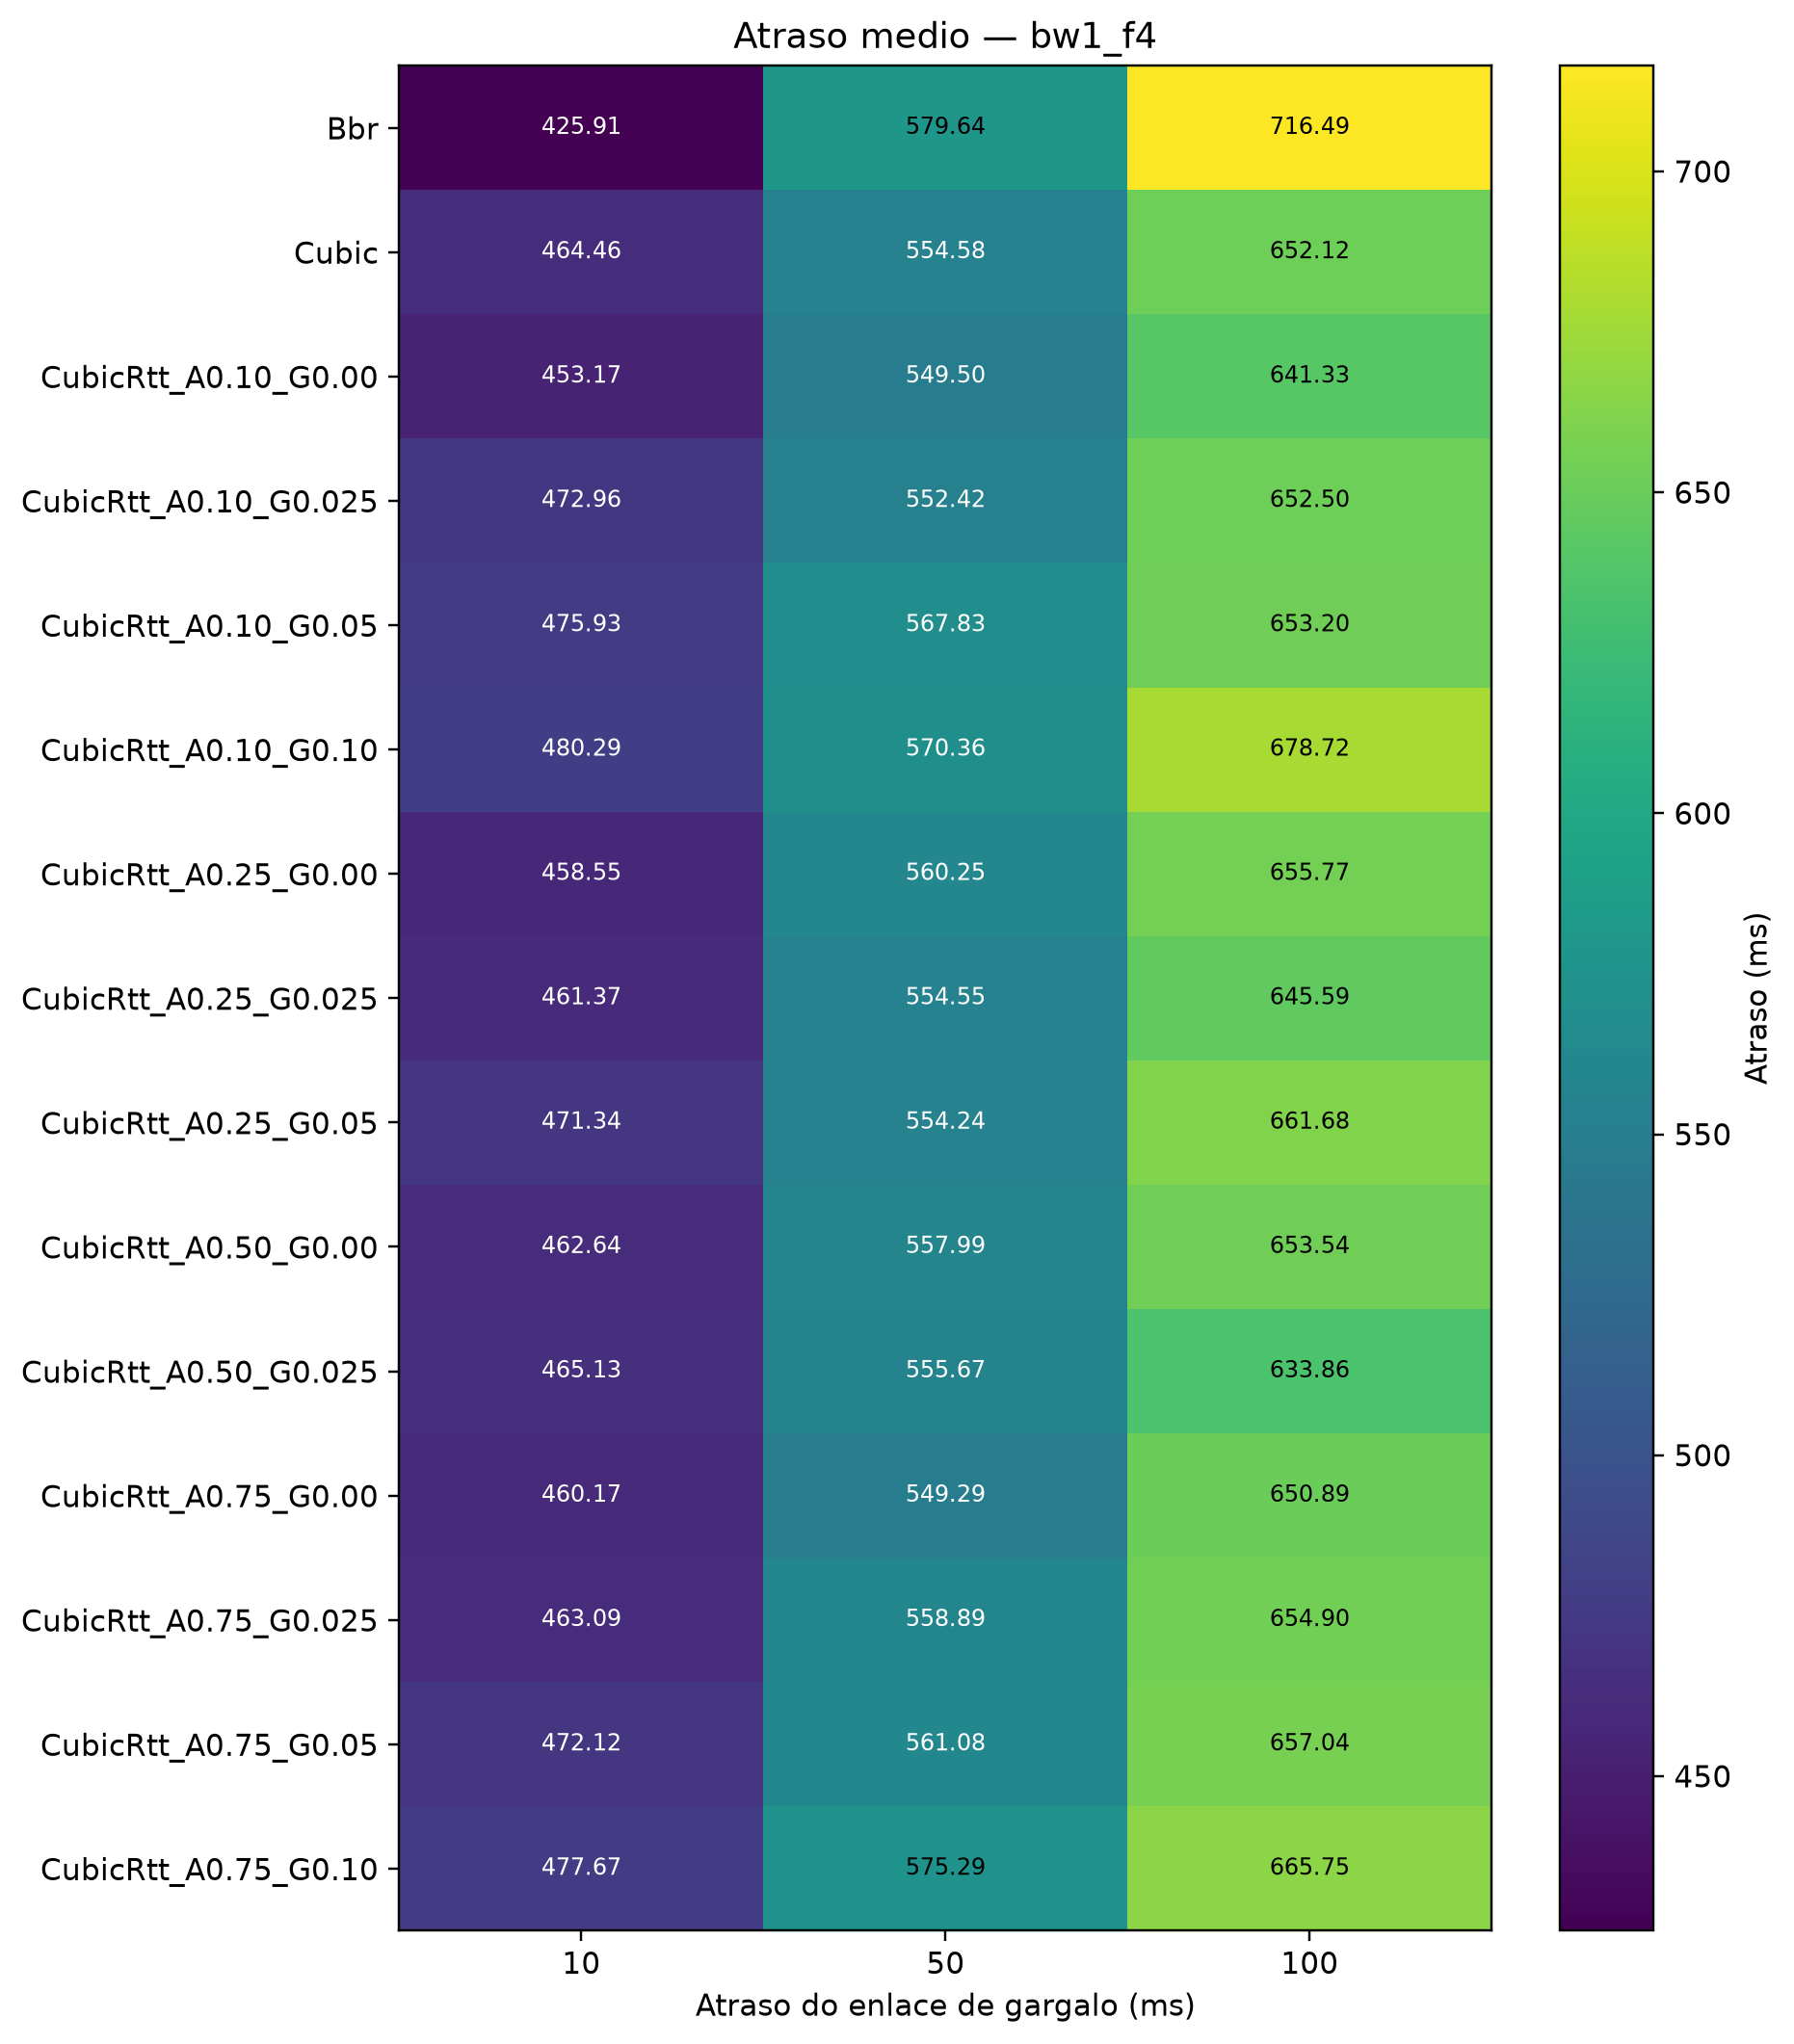
\includegraphics[width=0.88\textwidth]{bw1_f4_avg_delay_ms.png}
\caption{Atraso médio no cenário \texttt{bw1\_f4}.}
\label{fig:bw1-delay}
\end{figure}

\begin{figure}[p]
\centering
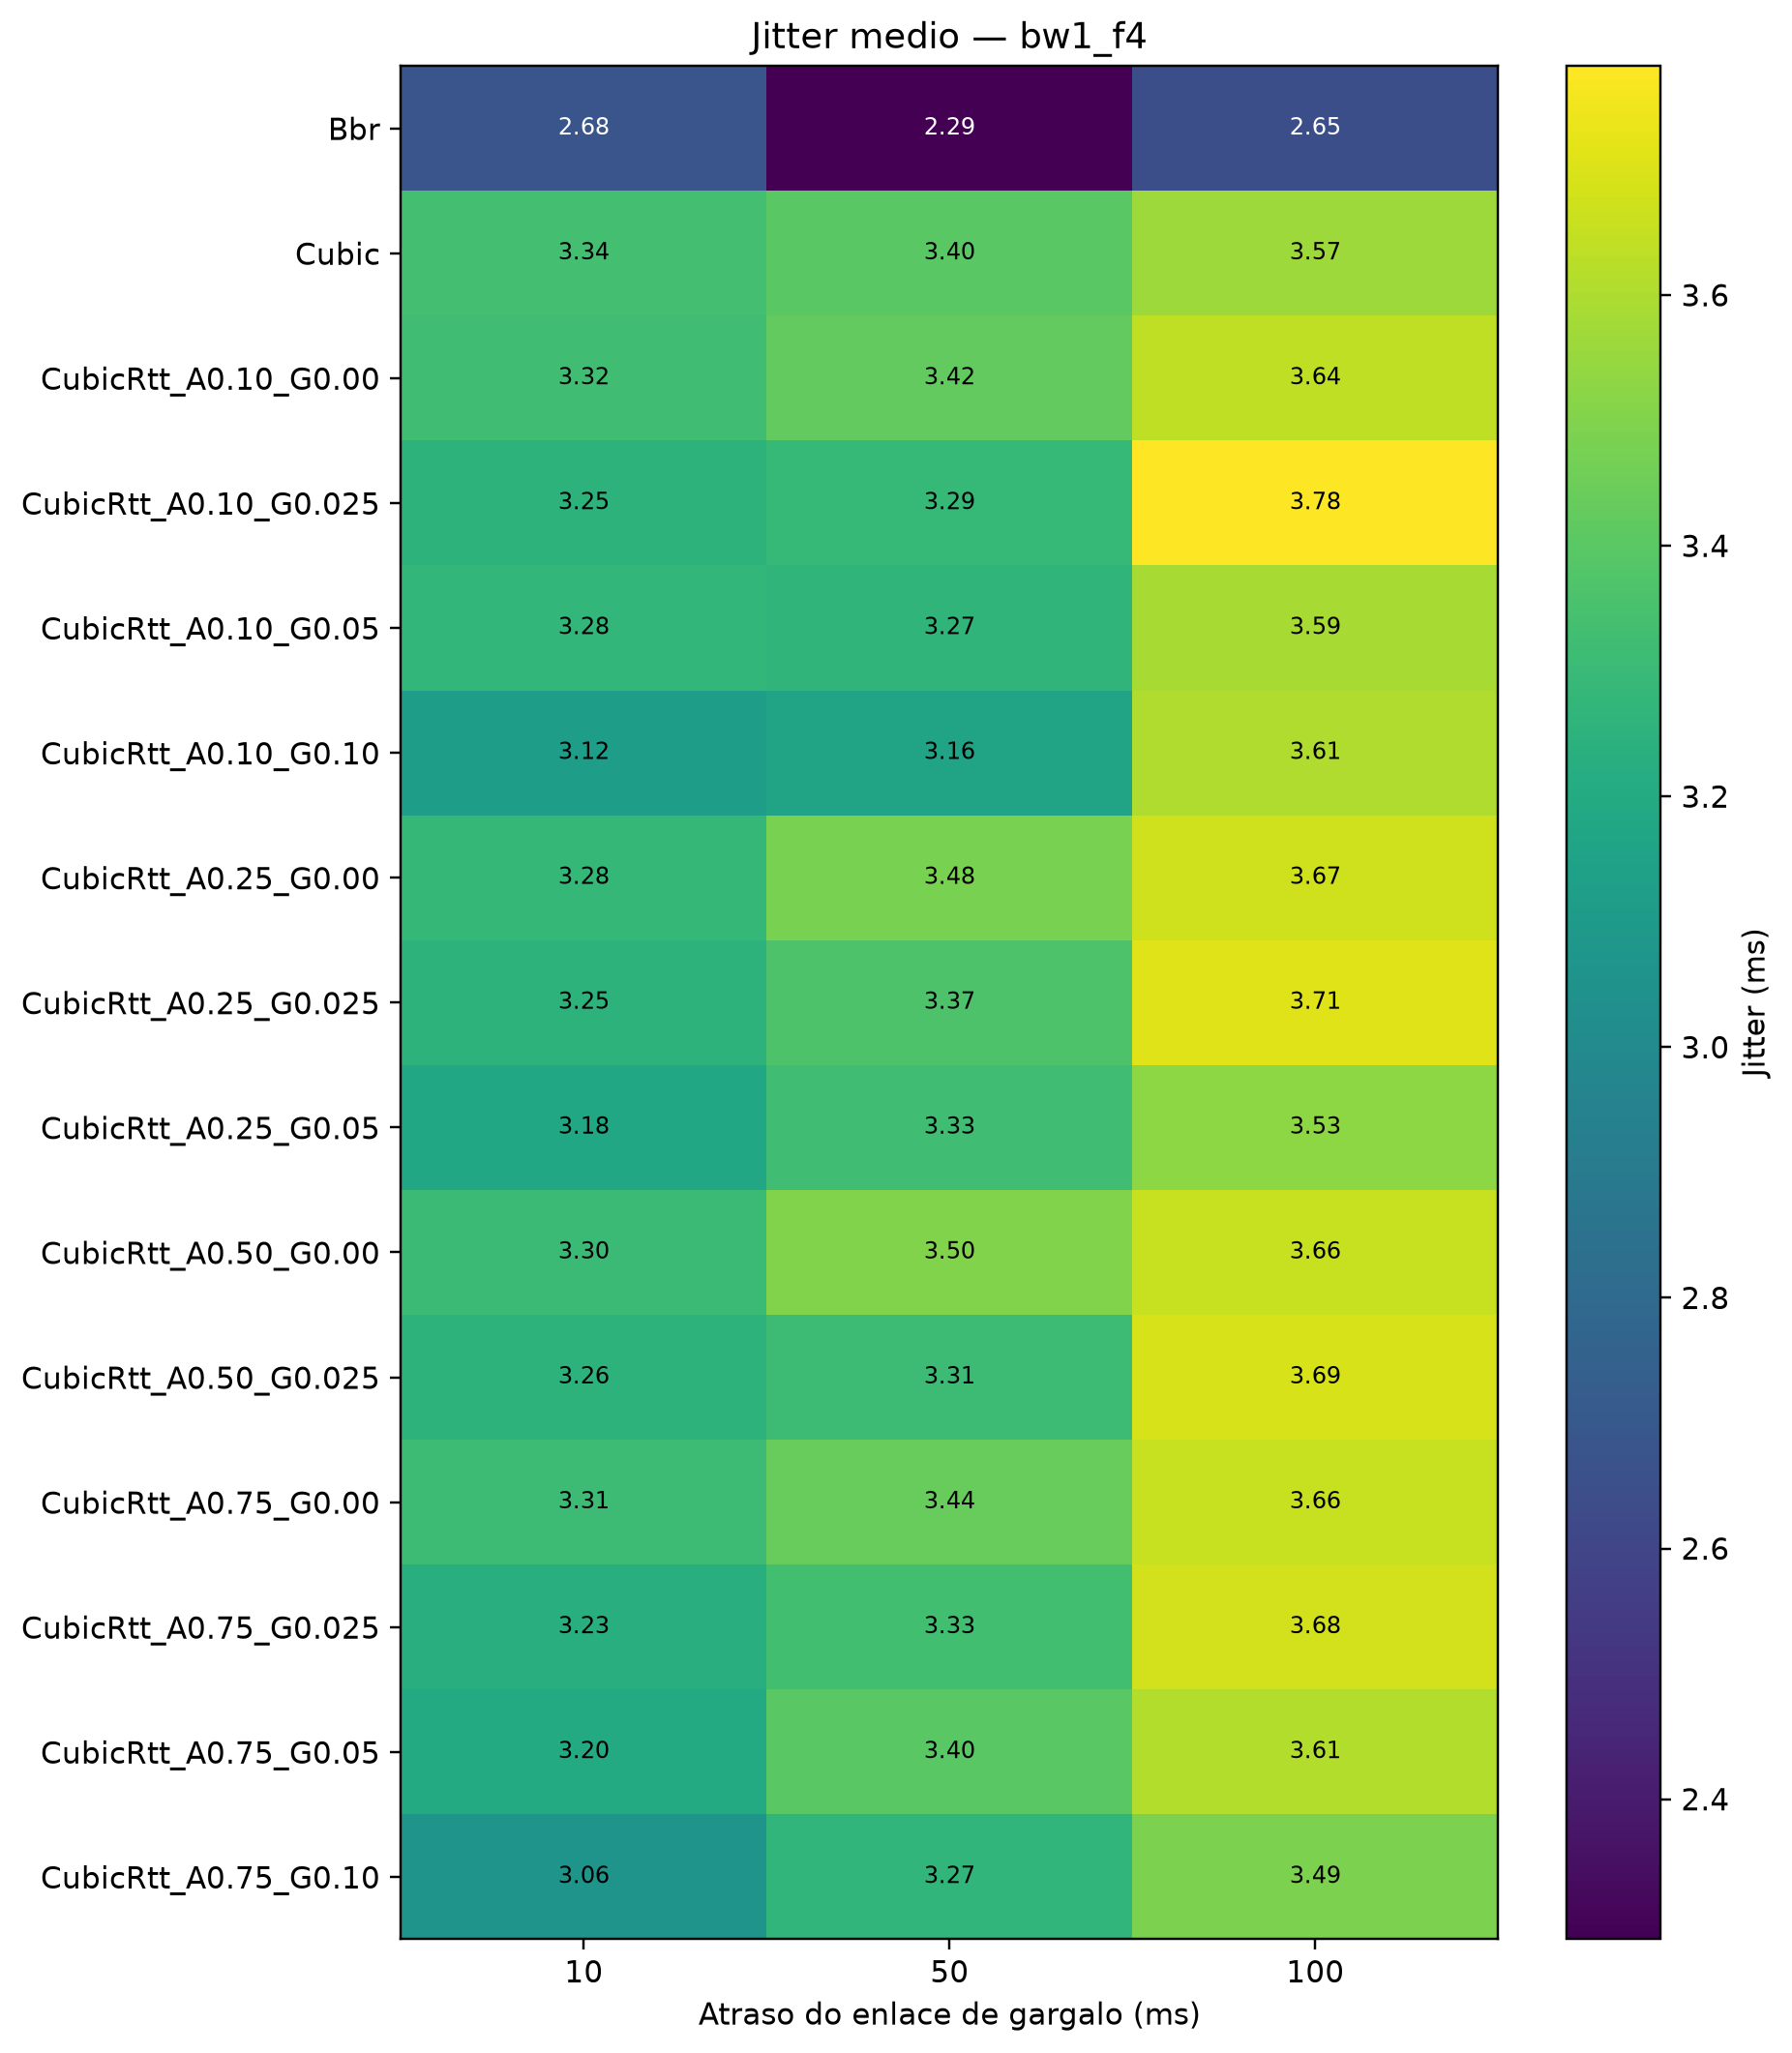
\includegraphics[width=0.88\textwidth]{bw1_f4_avg_jitter_ms.png}
\caption{Jitter médio no cenário \texttt{bw1\_f4}.}
\label{fig:bw1-jitter}
\end{figure}

\begin{figure}[p]
\centering
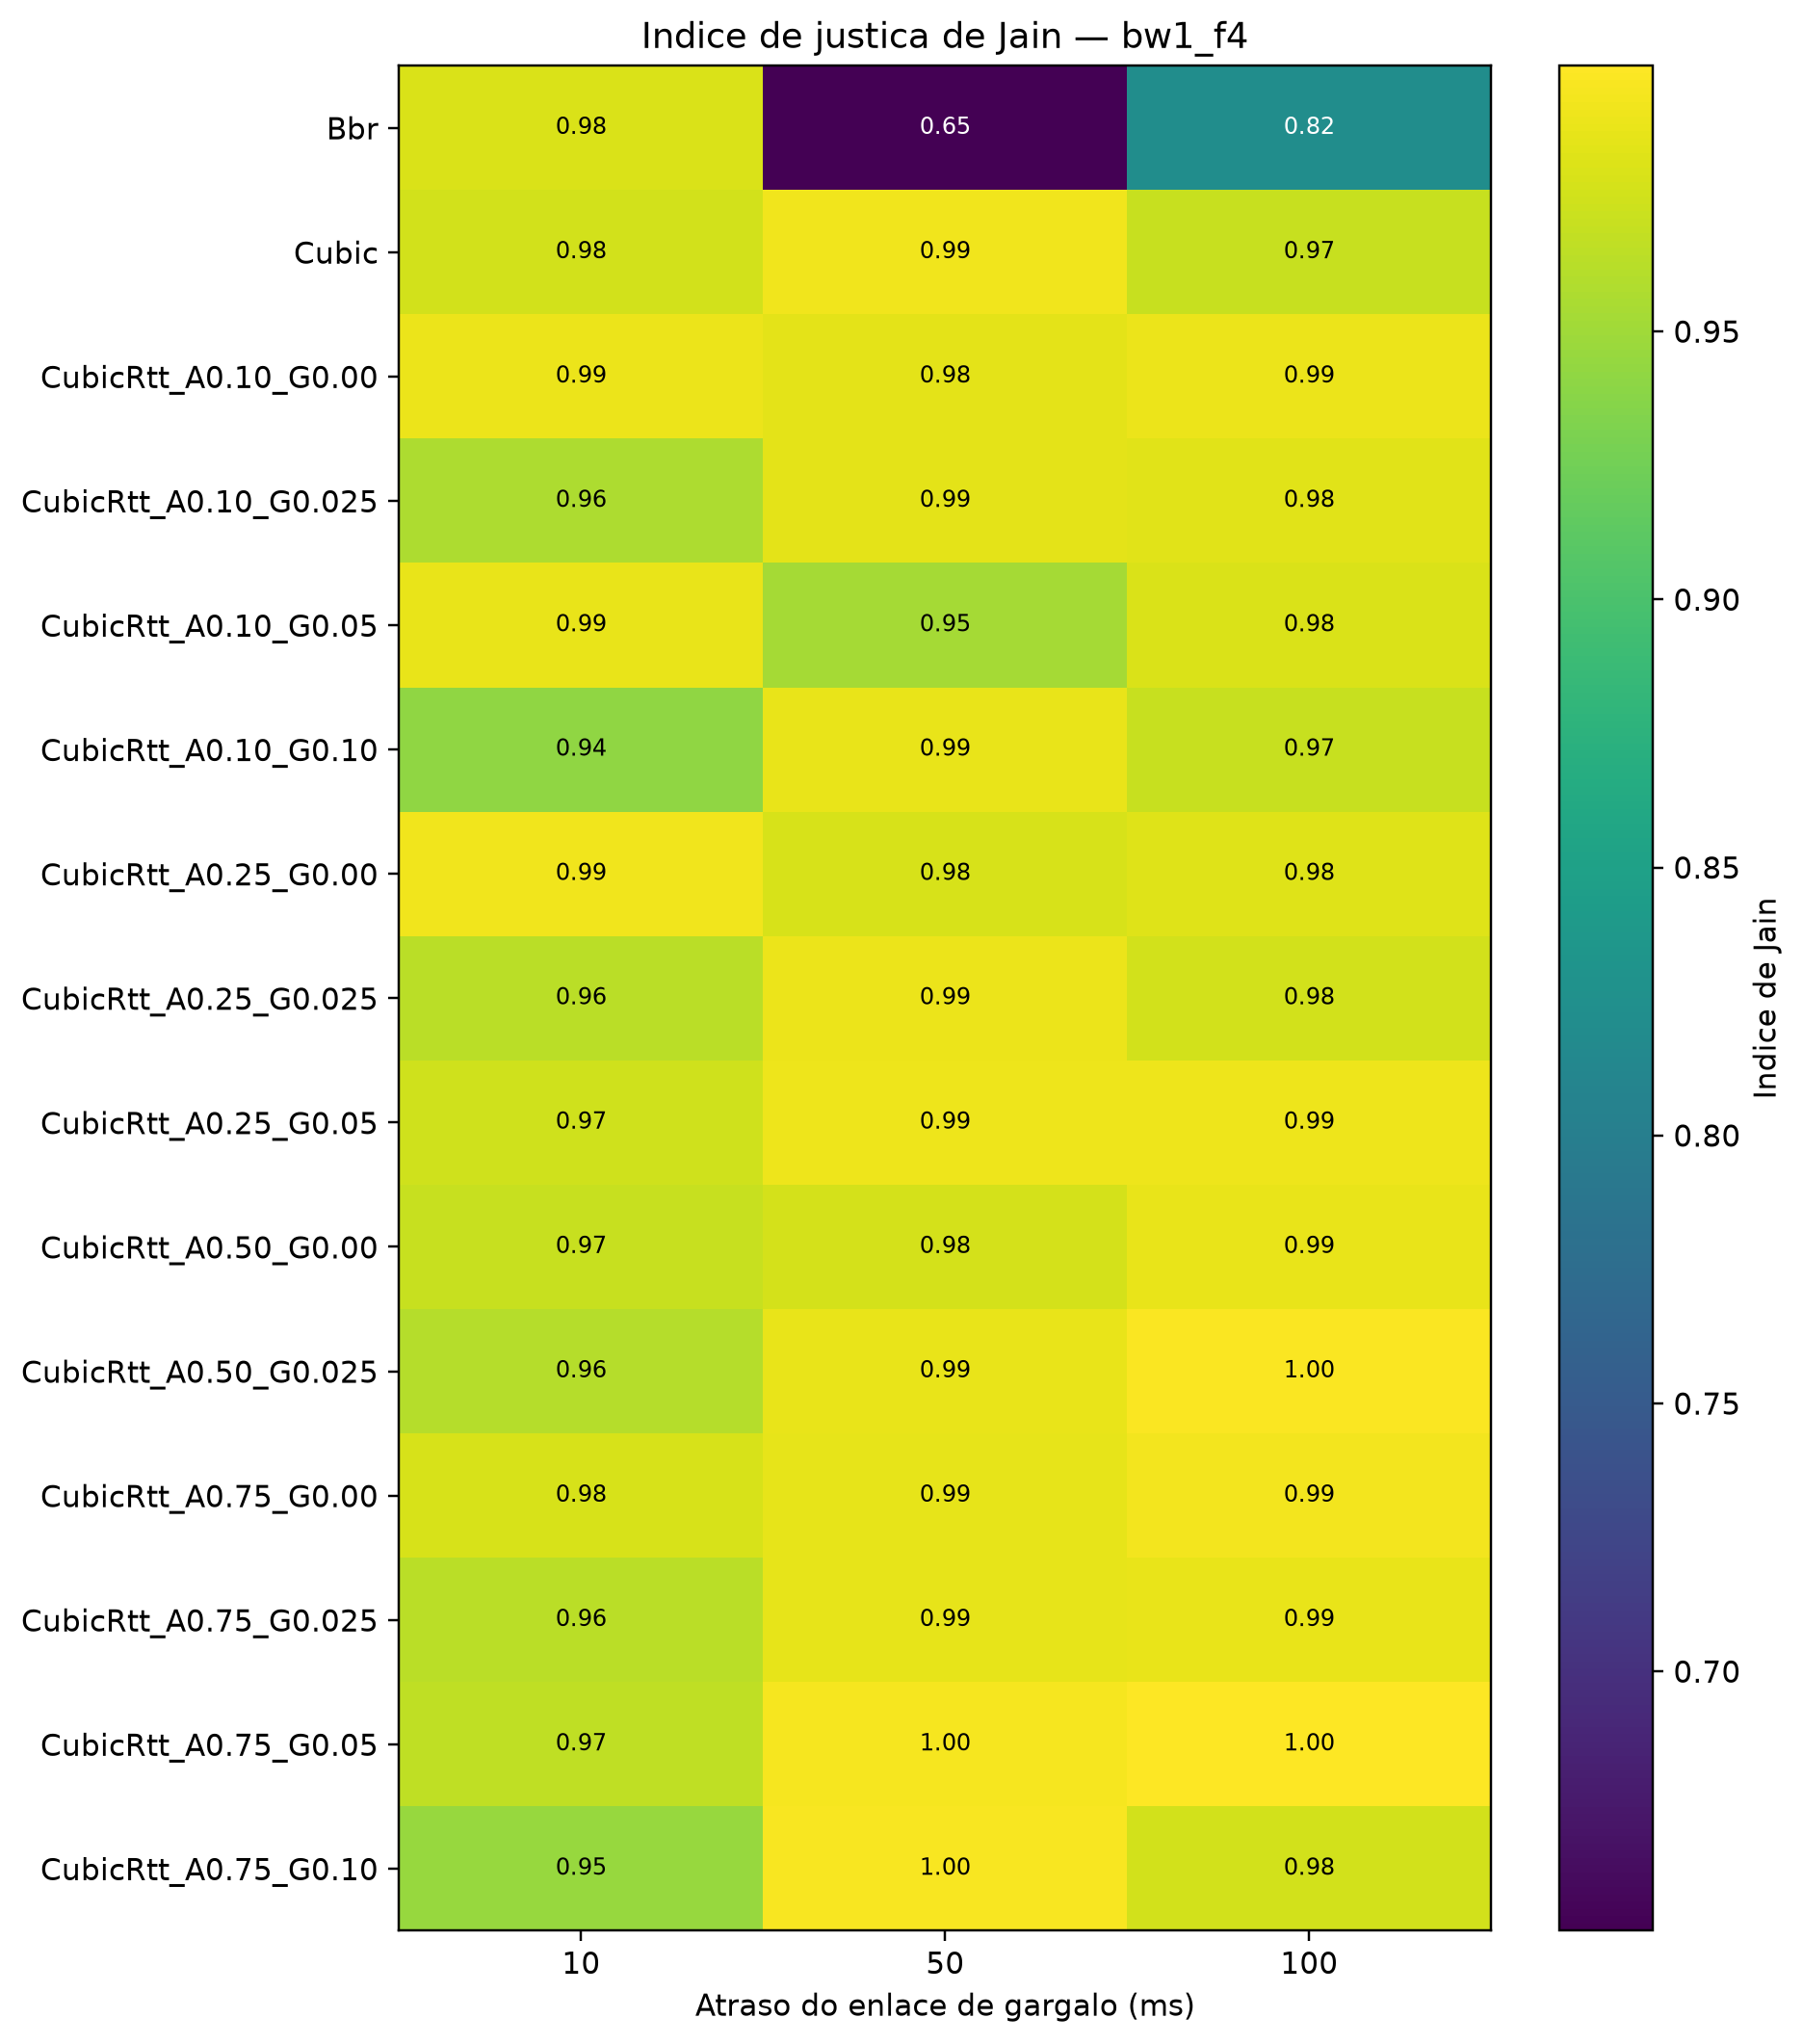
\includegraphics[width=0.88\textwidth]{bw1_f4_jain_fairness.png}
\caption{Índice de Justiça de Jain no cenário \texttt{bw1\_f4}.}
\label{fig:bw1-jain}
\end{figure}

\subsection{Cenário bw2\_f8}

\begin{figure}[p]
\centering
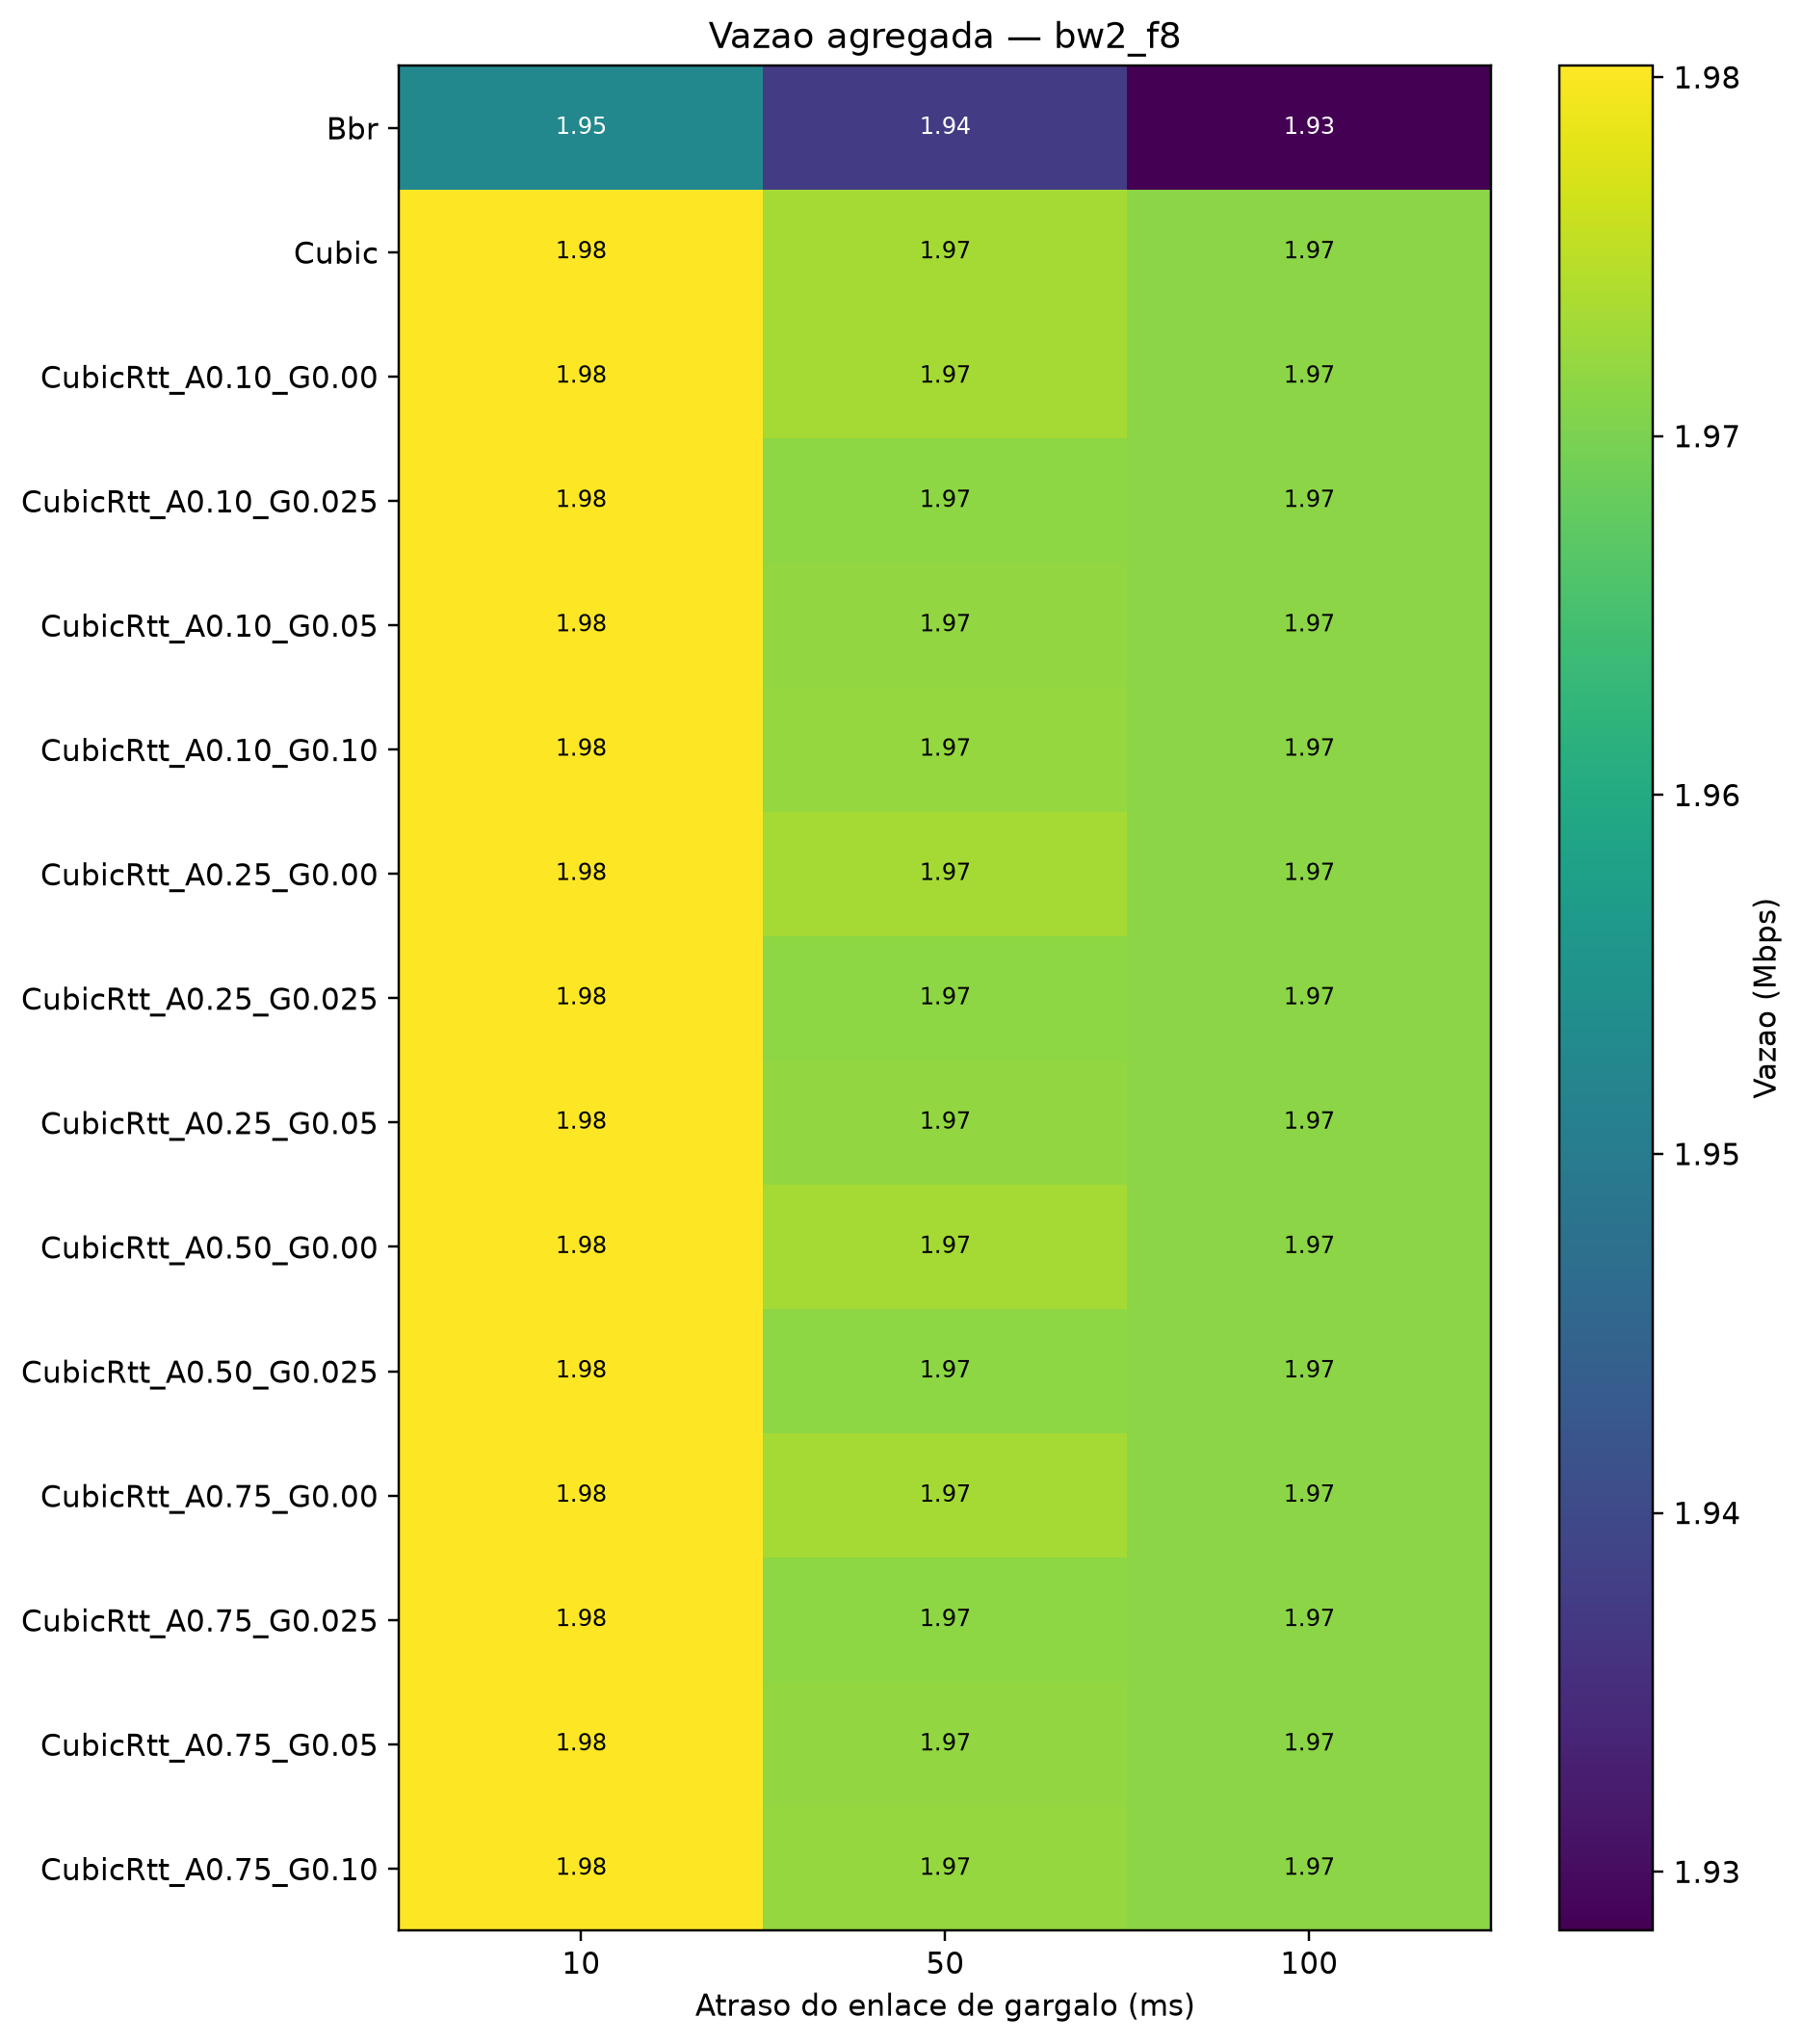
\includegraphics[width=0.88\textwidth]{bw2_f8_throughput_mbps.png}
\caption{Vazão agregada no cenário \texttt{bw2\_f8}.}
\label{fig:bw2-throughput}
\end{figure}

\begin{figure}[p]
\centering
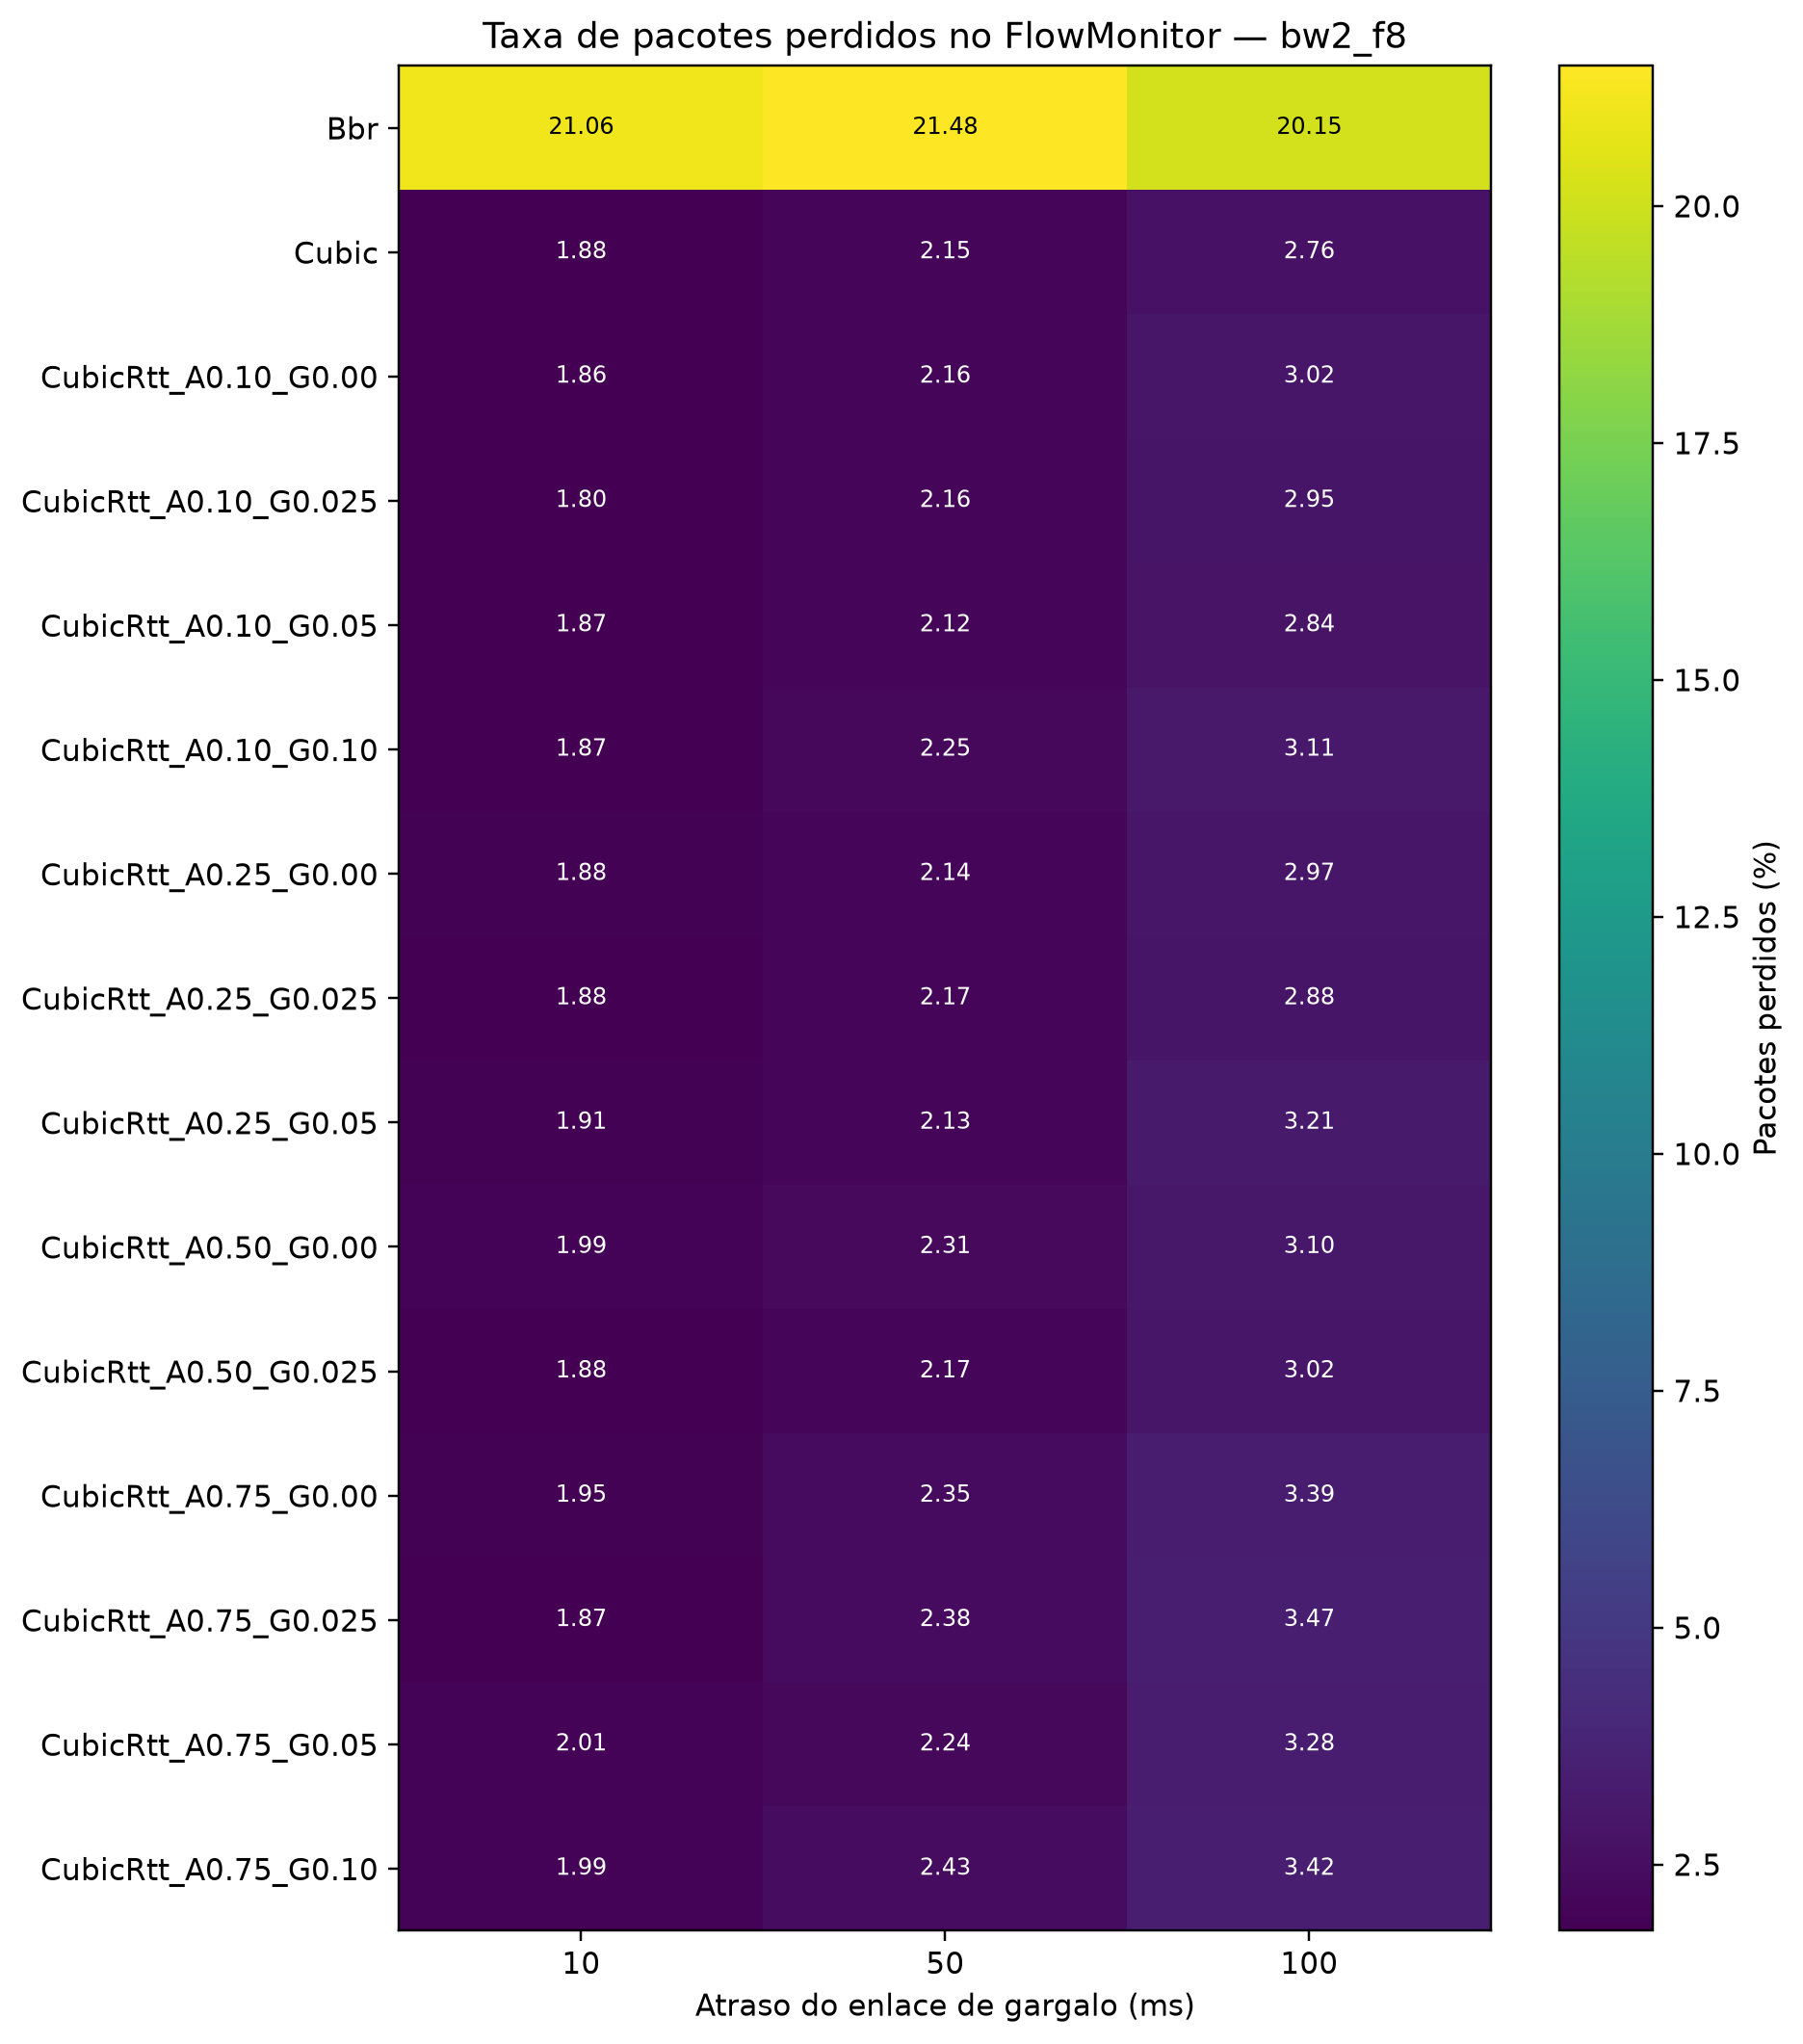
\includegraphics[width=0.88\textwidth]{bw2_f8_loss_rate_pct.png}
\caption{Taxa de perda de pacotes no cenário \texttt{bw2\_f8}.}
\label{fig:bw2-loss}
\end{figure}

\begin{figure}[p]
\centering
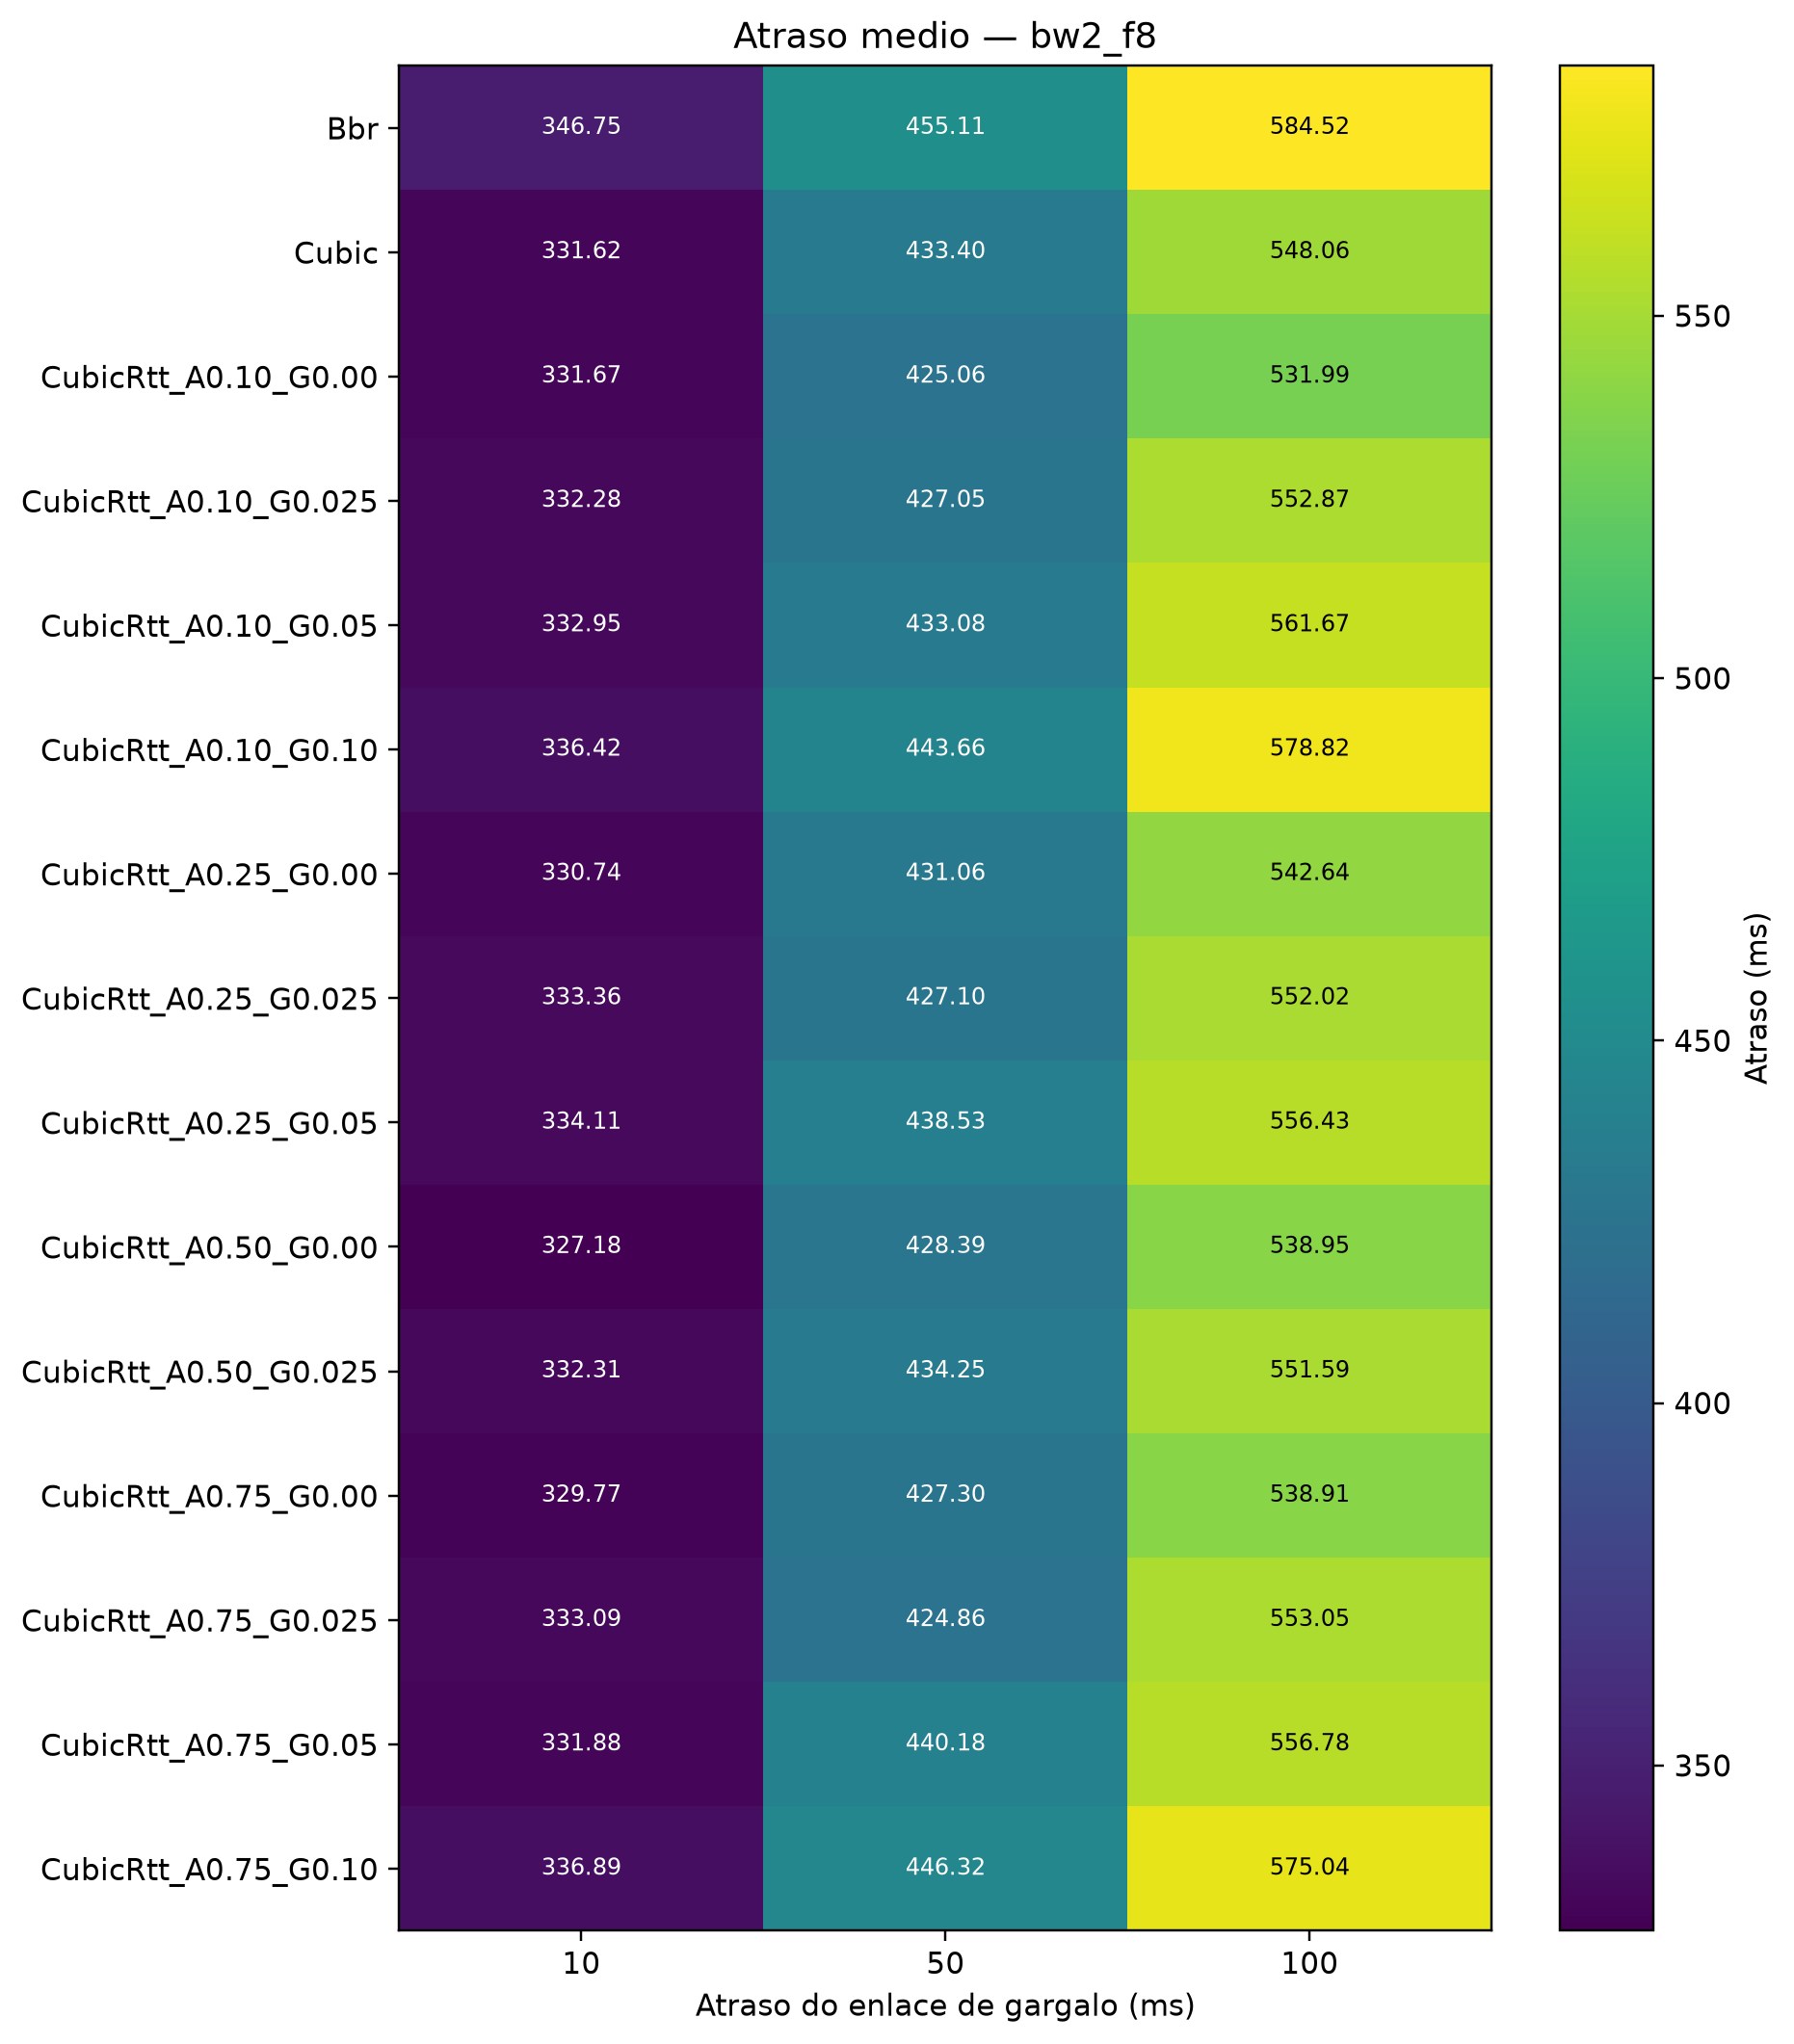
\includegraphics[width=0.88\textwidth]{bw2_f8_avg_delay_ms.png}
\caption{Atraso médio no cenário \texttt{bw2\_f8}.}
\label{fig:bw2-delay}
\end{figure}

\begin{figure}[p]
\centering
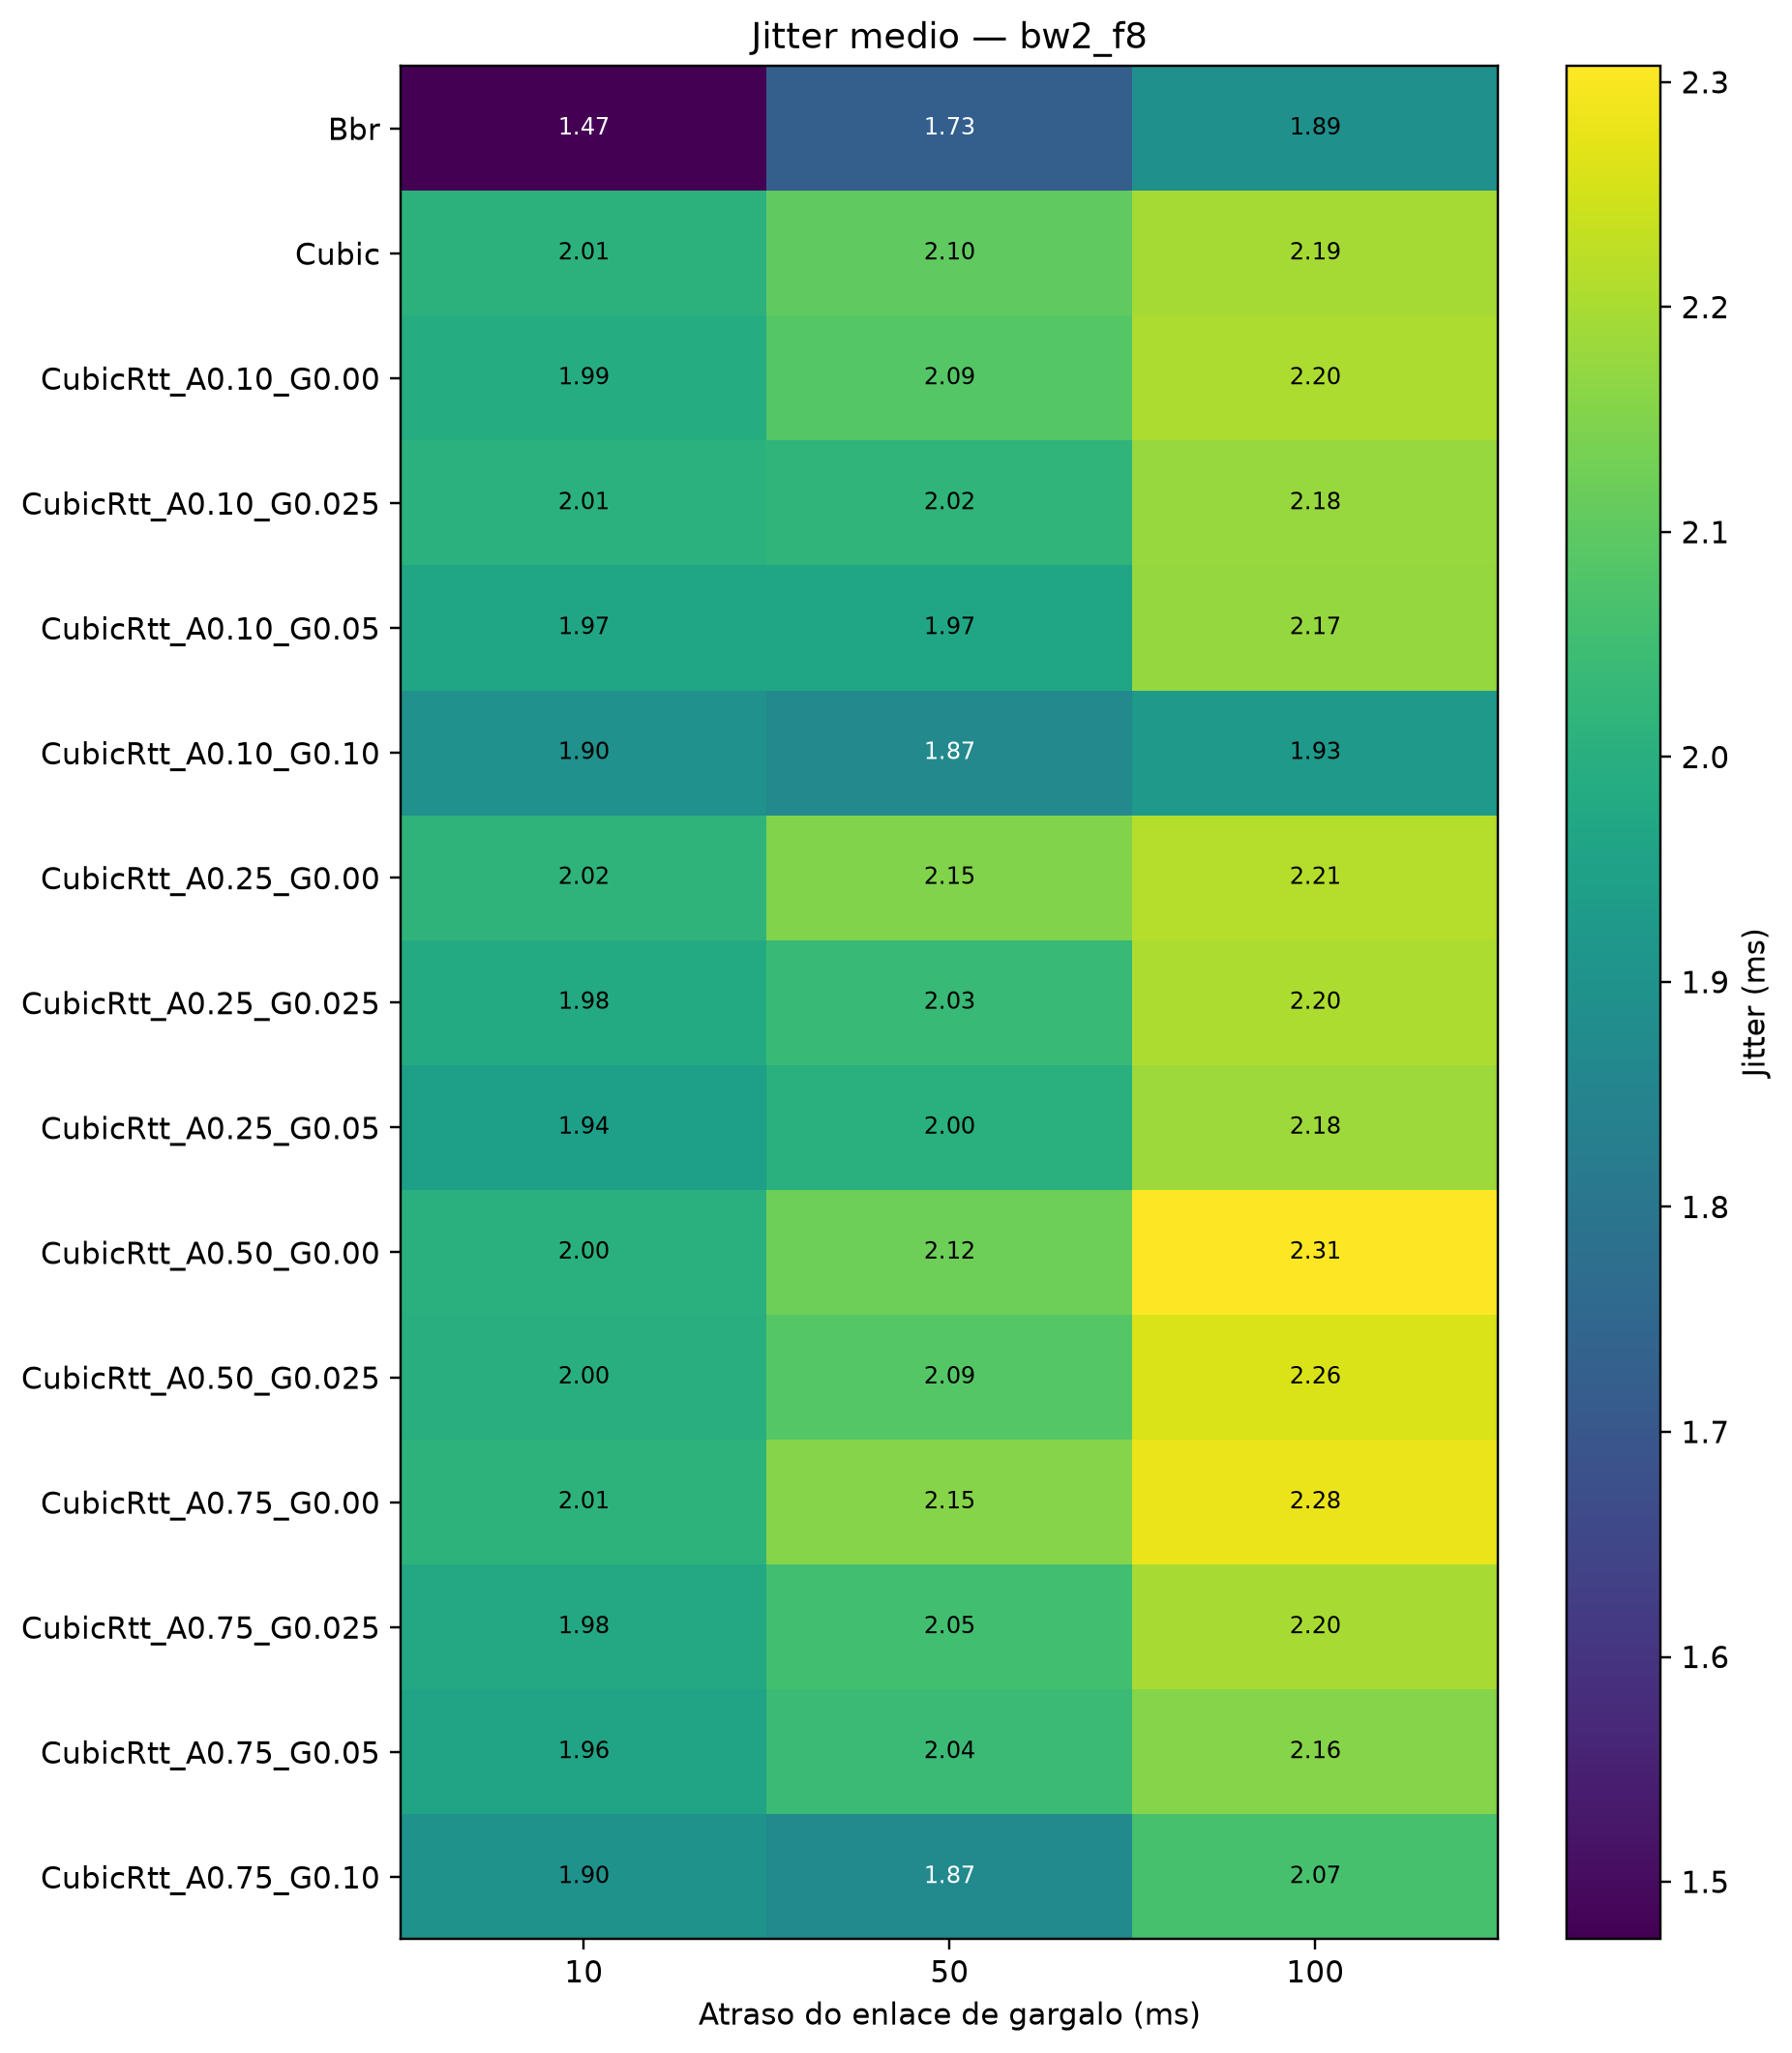
\includegraphics[width=0.88\textwidth]{bw2_f8_avg_jitter_ms.png}
\caption{Jitter médio no cenário \texttt{bw2\_f8}.}
\label{fig:bw2-jitter}
\end{figure}

\begin{figure}[p]
\centering
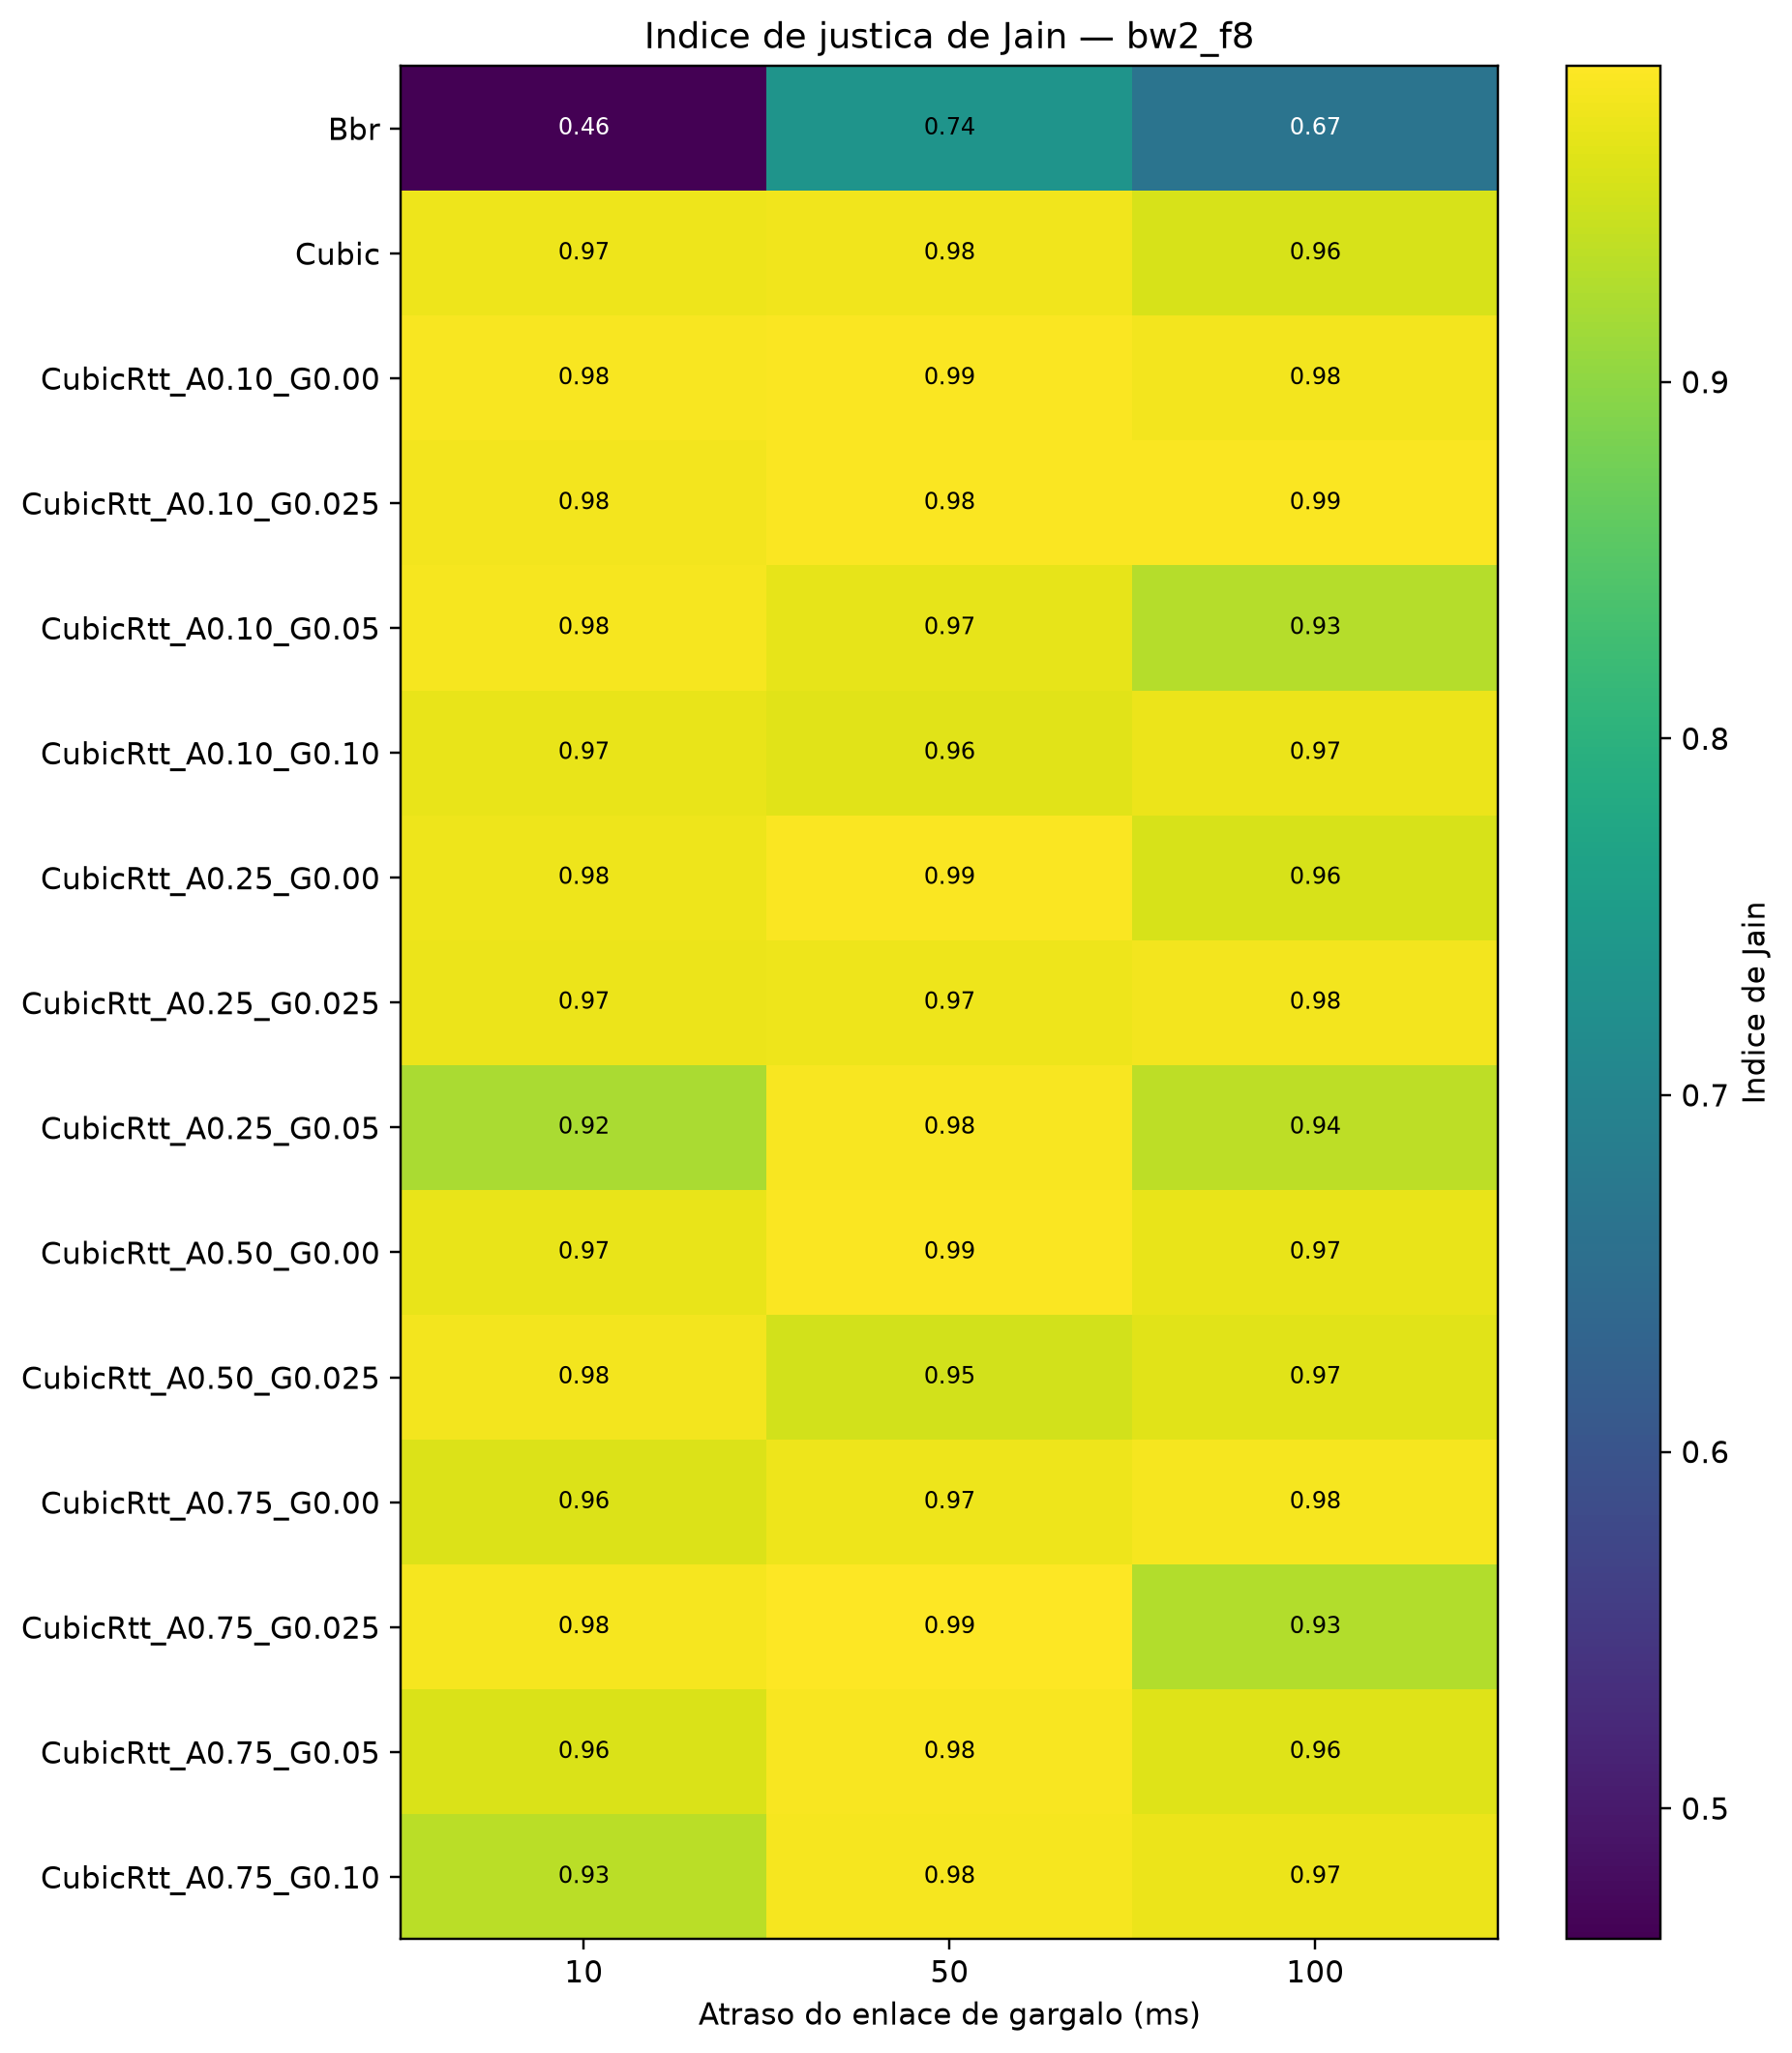
\includegraphics[width=0.88\textwidth]{bw2_f8_jain_fairness.png}
\caption{Índice de Justiça de Jain no cenário \texttt{bw2\_f8}.}
\label{fig:bw2-jain}
\end{figure}

\section{Rastros Temporais da Campanha de Coexistência}
\label{ap:traces}

Os gráficos apresentam exemplos da evolução temporal da janela de congestionamento e do RTT dos oito fluxos simultâneos. Eles complementam a análise agregada do Capítulo~\ref{cap:resultados}, permitindo observar a dinâmica das conexões durante as execuções.

\subsection{Atraso de gargalo de 10 ms}

\begin{figure}[p]
\centering
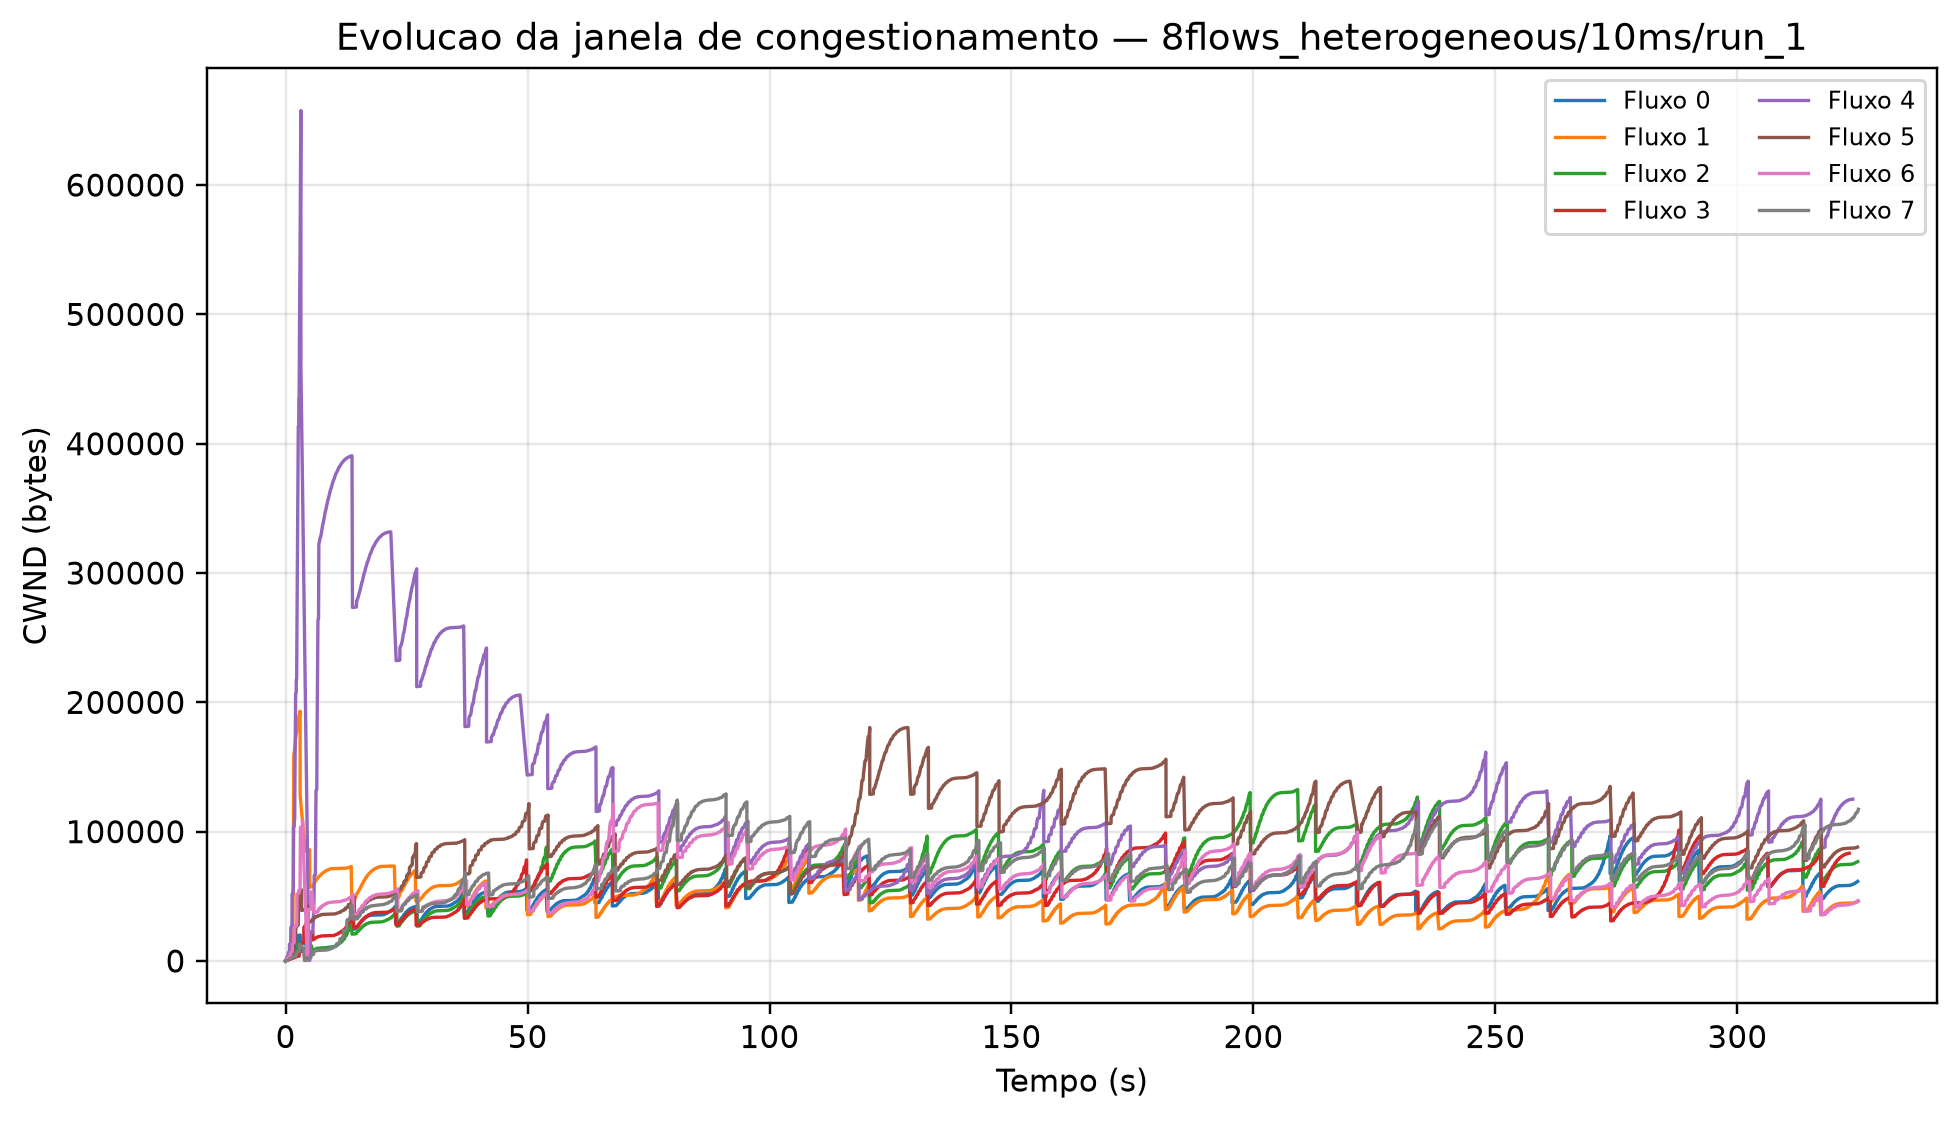
\includegraphics[width=\textwidth]{8flows_heterogeneous_10ms_run_1_cwnd.png}
\caption{Evolução da janela de congestionamento dos oito fluxos, com gargalo de 10 ms.}
\label{fig:trace-cwnd-10}
\end{figure}

\begin{figure}[p]
\centering
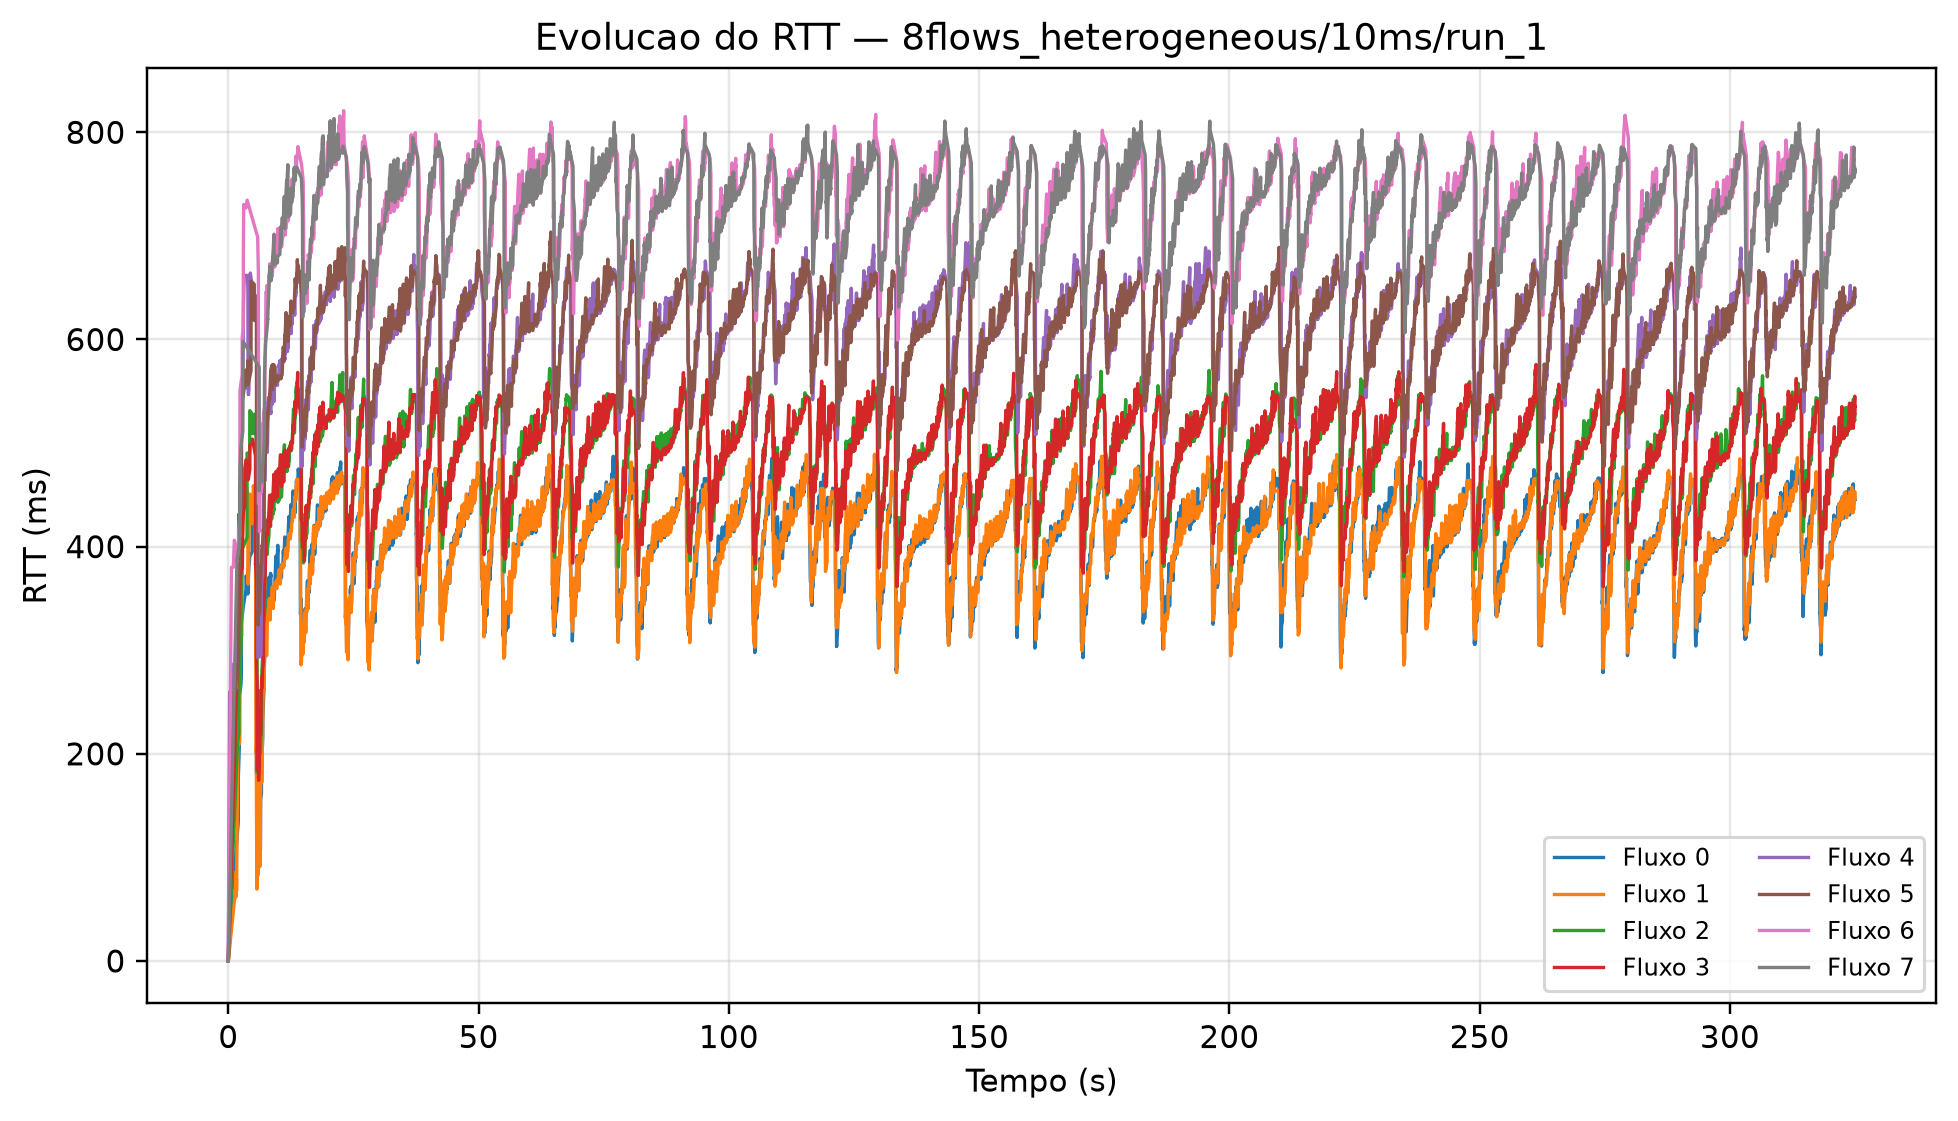
\includegraphics[width=\textwidth]{8flows_heterogeneous_10ms_run_1_rtt.png}
\caption{Evolução do RTT dos oito fluxos, com gargalo de 10 ms.}
\label{fig:trace-rtt-10}
\end{figure}

\subsection{Atraso de gargalo de 50 ms}

\begin{figure}[p]
\centering
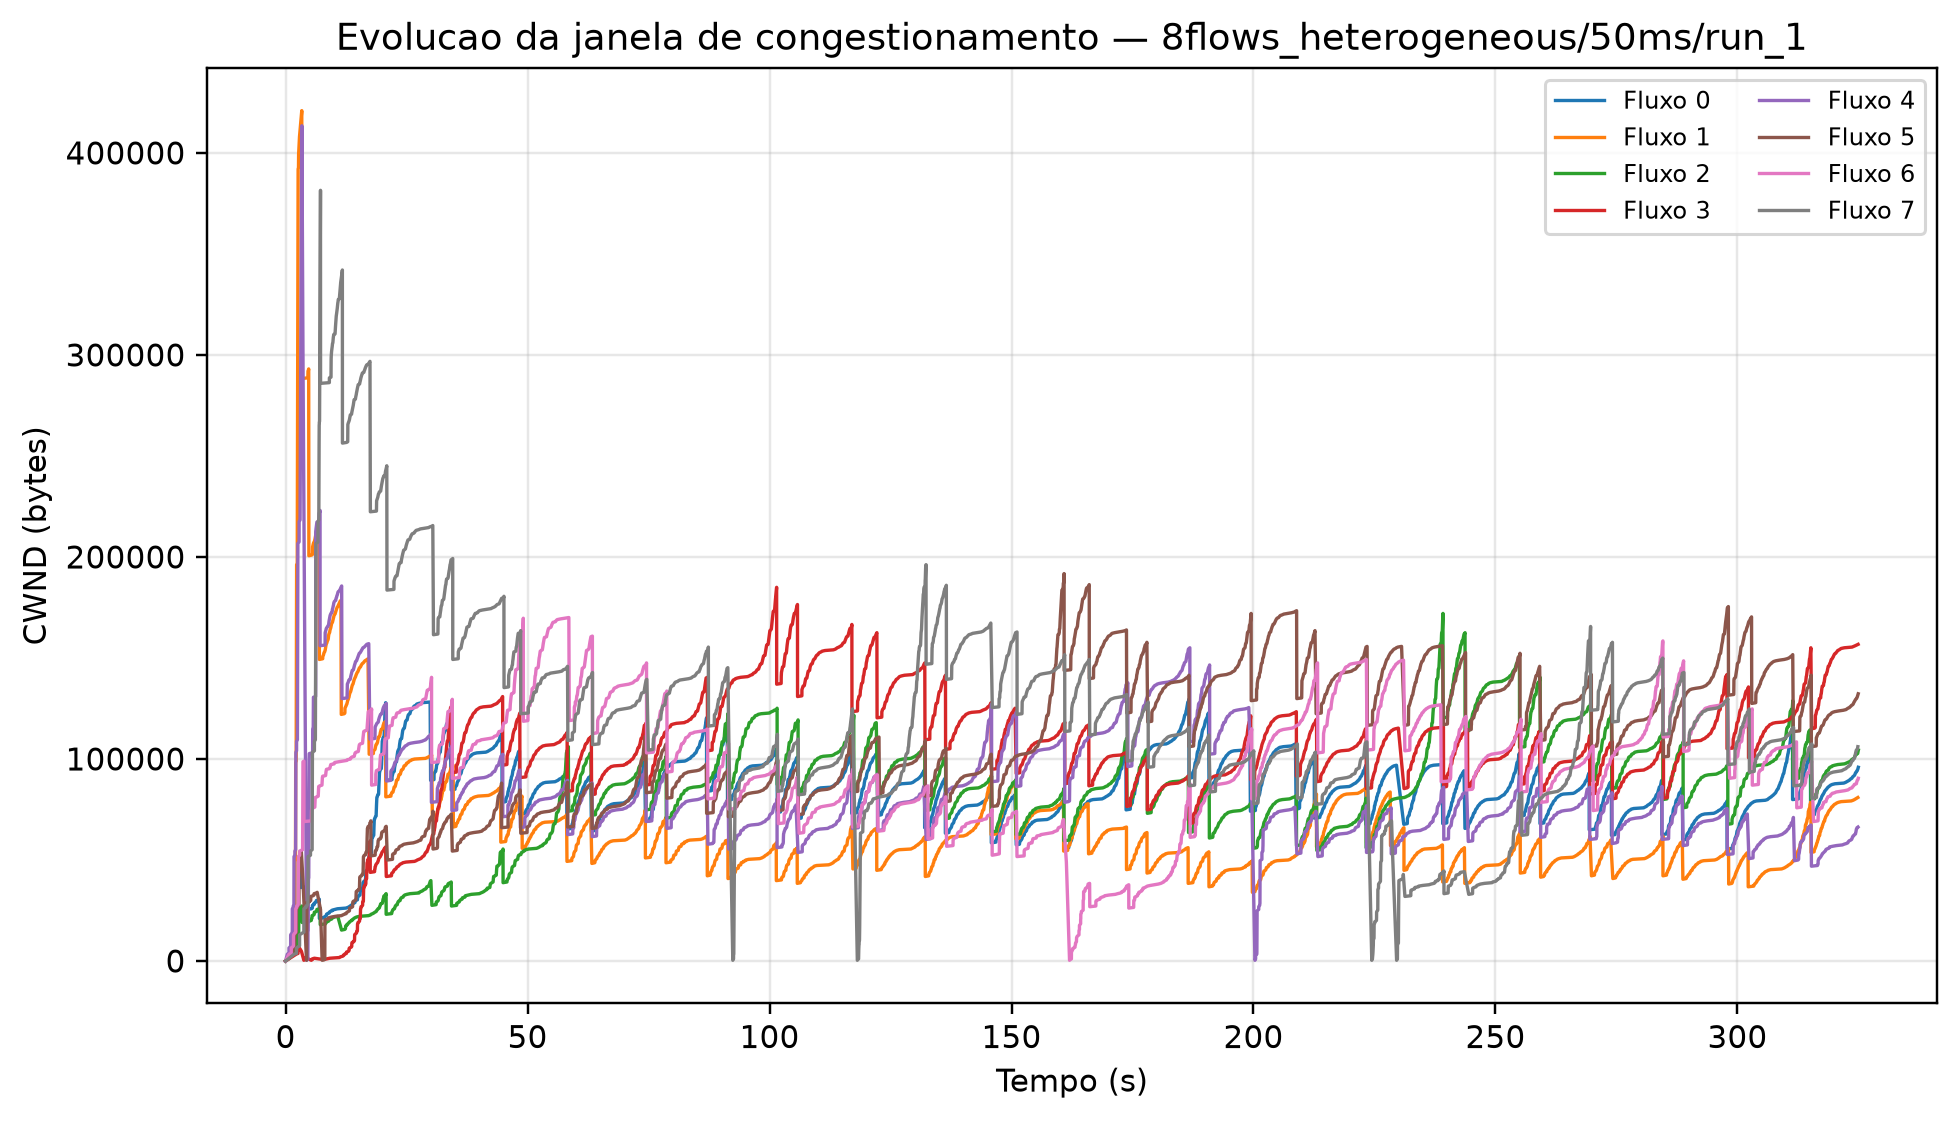
\includegraphics[width=\textwidth]{8flows_heterogeneous_50ms_run_1_cwnd.png}
\caption{Evolução da janela de congestionamento dos oito fluxos, com gargalo de 50 ms.}
\label{fig:trace-cwnd-50}
\end{figure}

\begin{figure}[p]
\centering
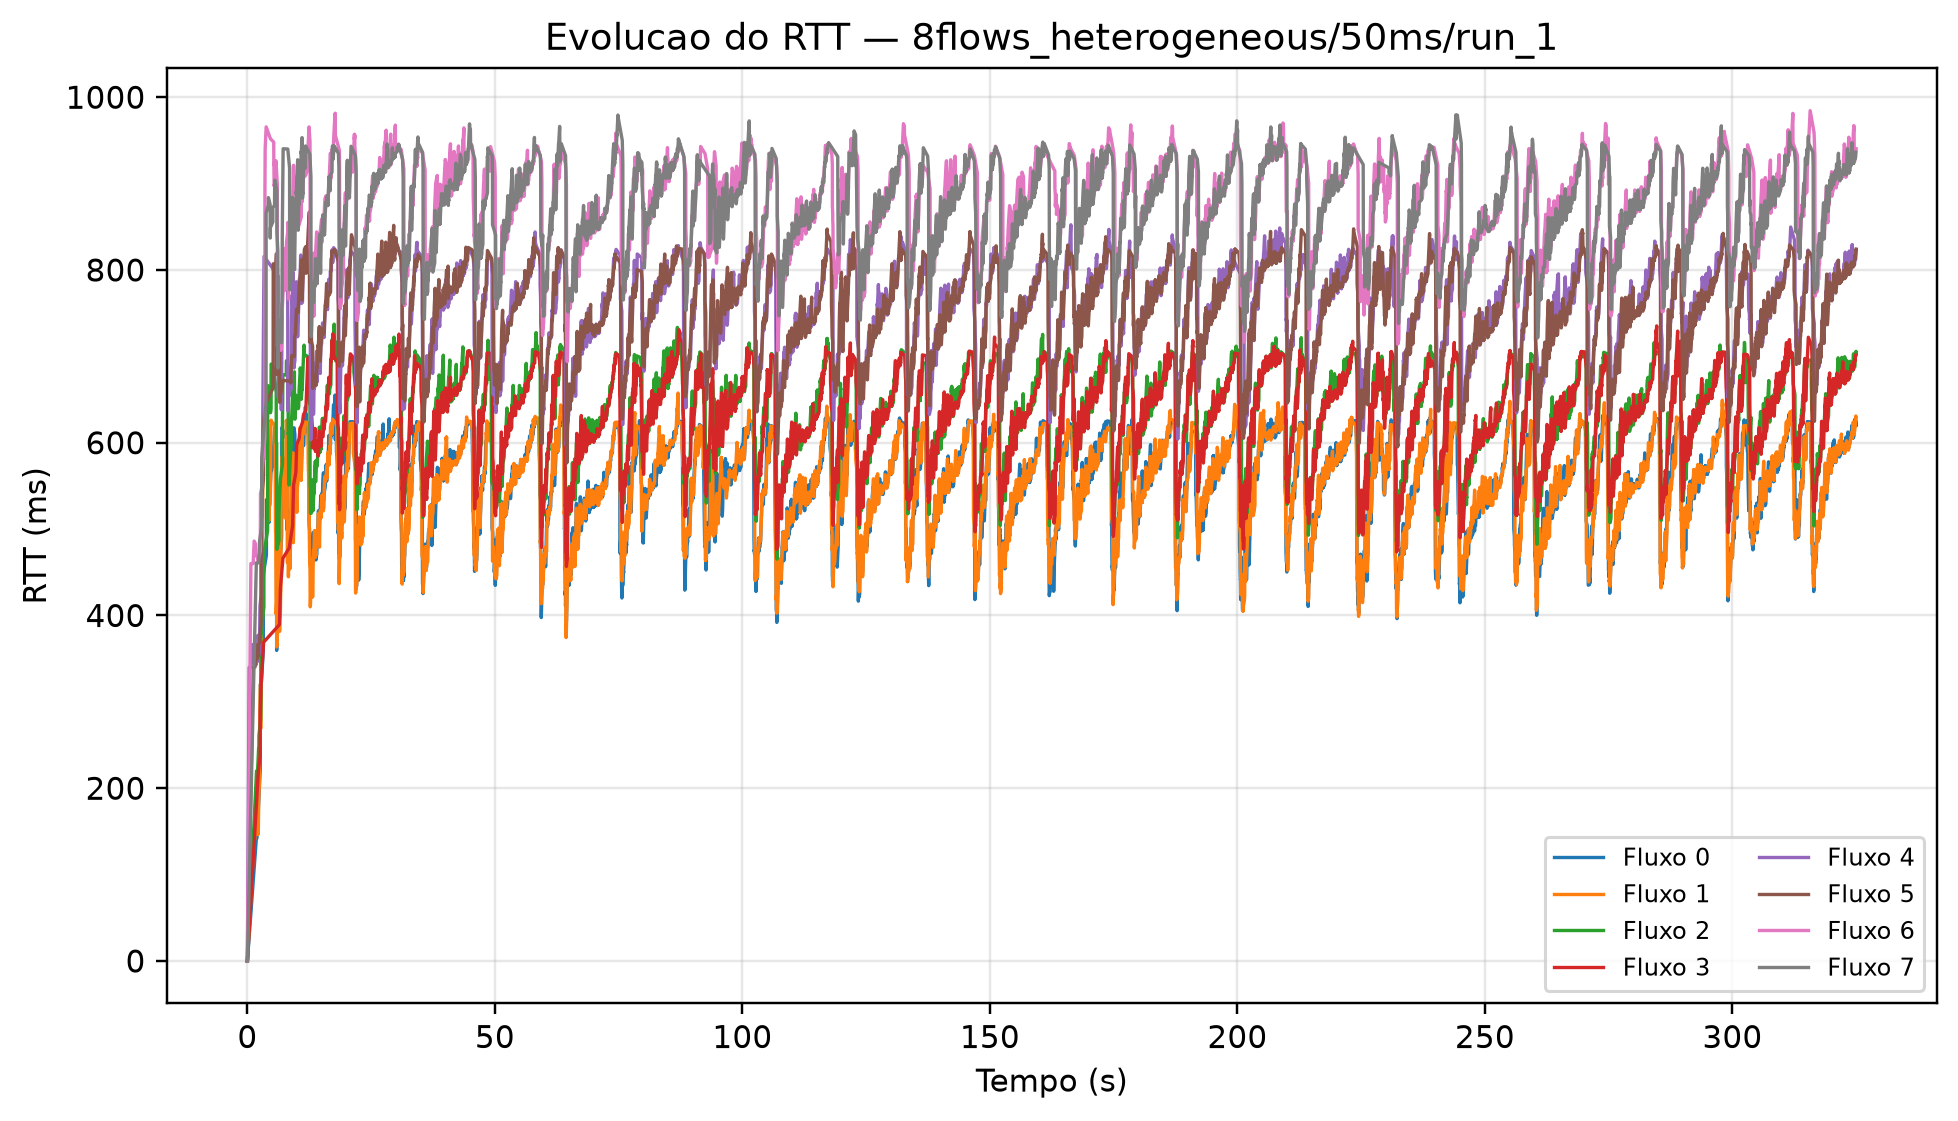
\includegraphics[width=\textwidth]{8flows_heterogeneous_50ms_run_1_rtt.png}
\caption{Evolução do RTT dos oito fluxos, com gargalo de 50 ms.}
\label{fig:trace-rtt-50}
\end{figure}

\subsection{Atraso de gargalo de 100 ms}

\begin{figure}[p]
\centering
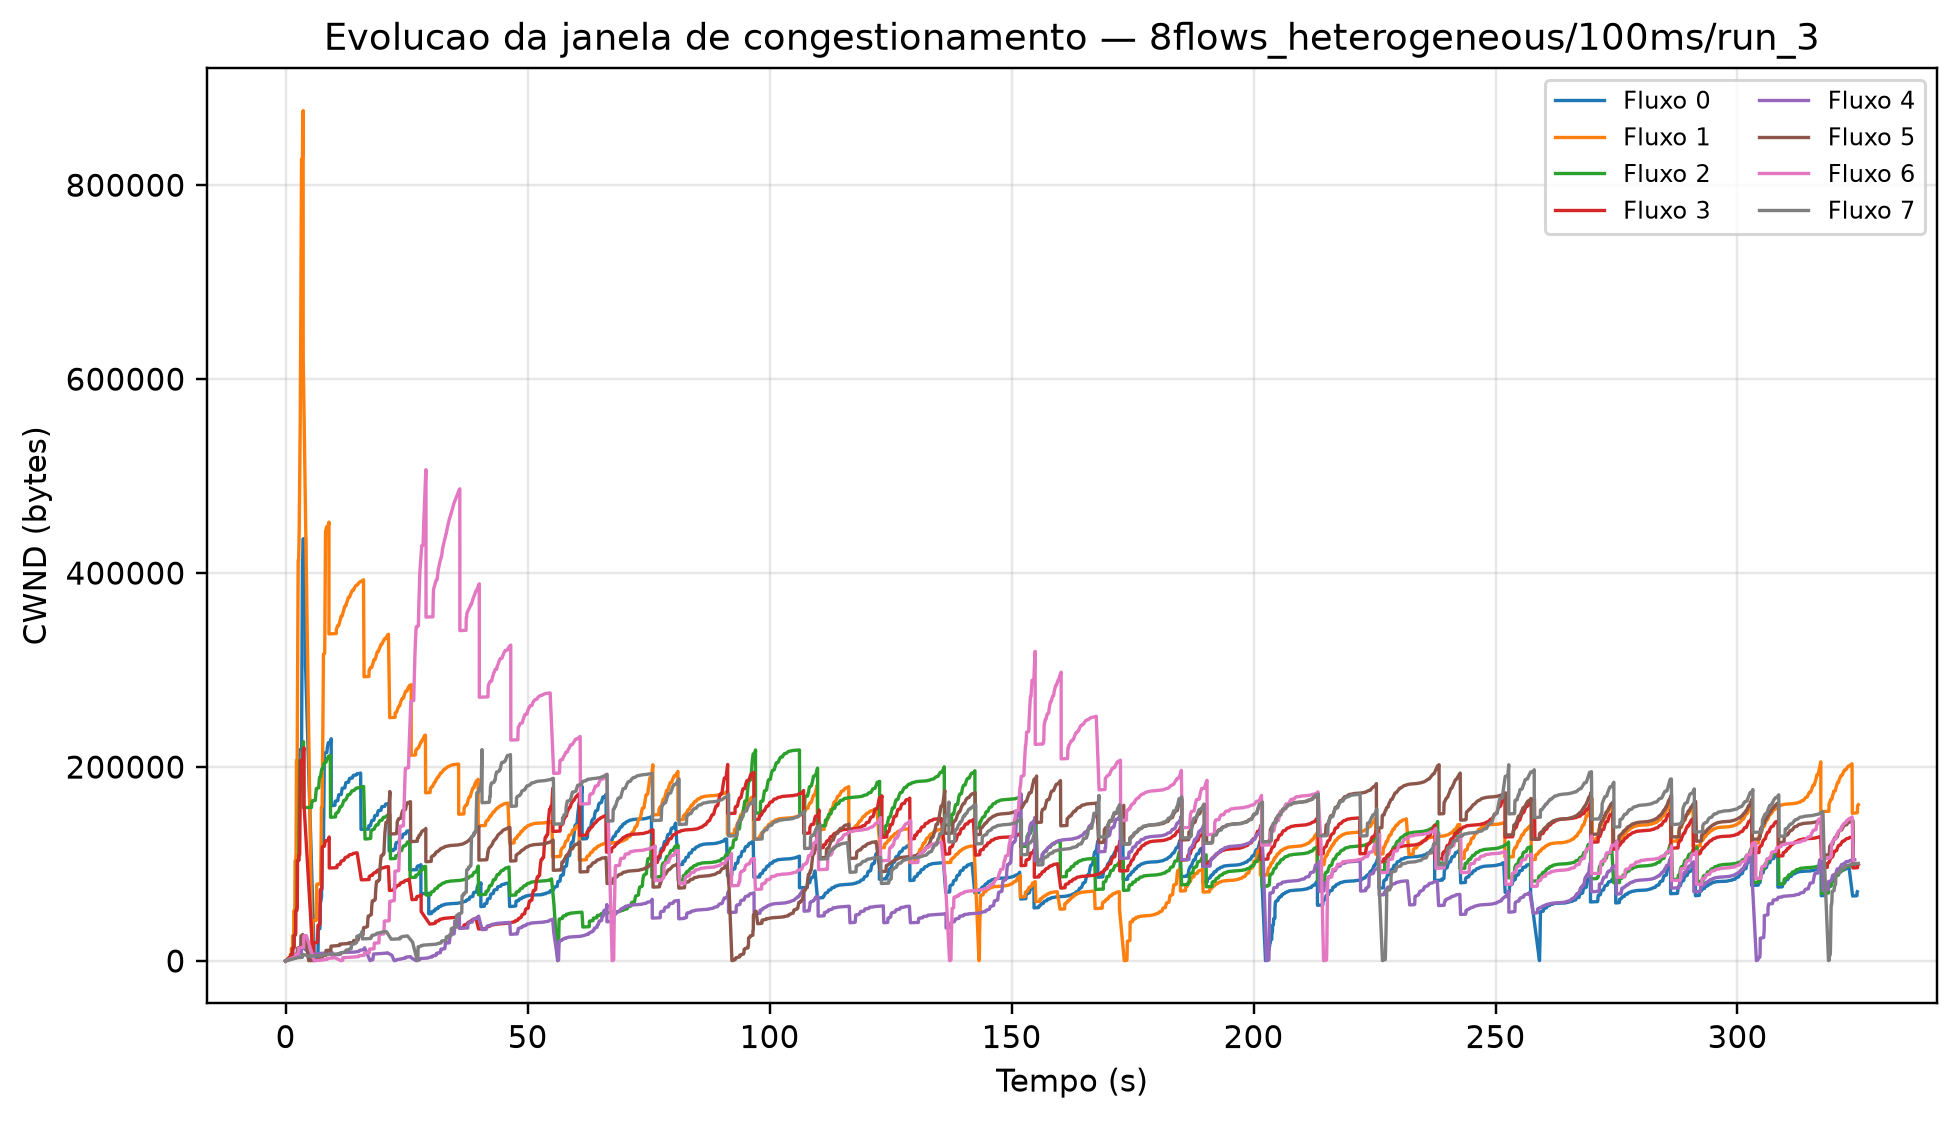
\includegraphics[width=\textwidth]{8flows_heterogeneous_100ms_run_3_cwnd.png}
\caption{Evolução da janela de congestionamento dos oito fluxos, com gargalo de 100 ms.}
\label{fig:trace-cwnd-100}
\end{figure}

\begin{figure}[p]
\centering
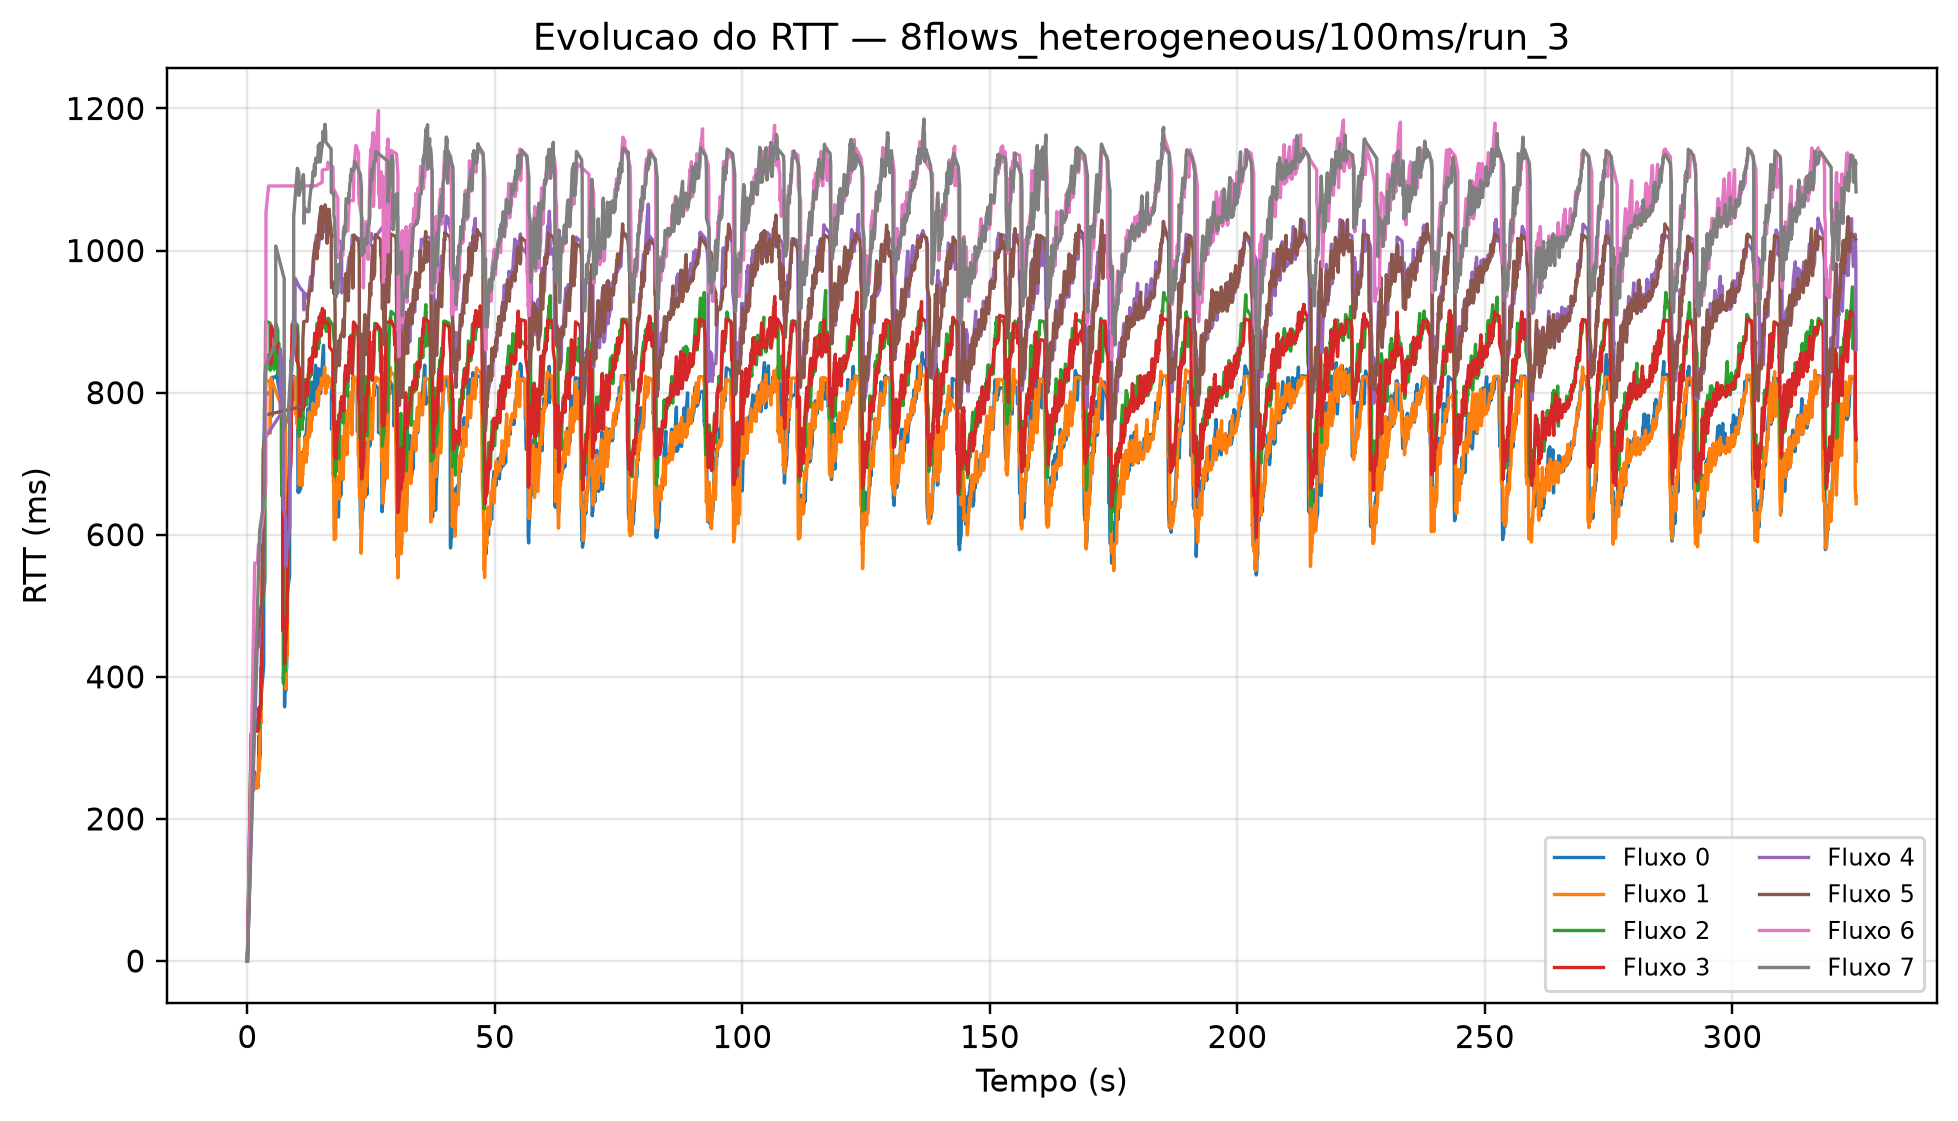
\includegraphics[width=\textwidth]{8flows_heterogeneous_100ms_run_3_rtt.png}
\caption{Evolução do RTT dos oito fluxos, com gargalo de 100 ms.}
\label{fig:trace-rtt-100}
\end{figure}

% --- Referências (ordem alfabética, estilo ABNT) ---
\begin{thebibliography}{99}

\bibitem{rfc5681}
ALLMAN, M.; PAXSON, V.; BLANTON, E.
\textbf{TCP Congestion Control}.
RFC 5681. IETF, set. 2009.

\bibitem{cardwell2017}
CARDWELL, N. et al.
BBR: Congestion-based congestion control.
\textbf{Communications of the ACM}, v. 60, n. 2, p. 58-66, 2017.

\bibitem{casas2022}
CASAS-VELASCO, D. M.; GRANELLI, F.; DA FONSECA, N. L. S.
Impact of background traffic on the BBR and CUBIC variants of the TCP protocol.
\textbf{IEEE Networking Letters}, v. 4, n. 3, p. 147-150, 2022.

\bibitem{rfc3393}
DEMICHELIS, C.; CHIMENTO, P.
\textbf{IP Packet Delay Variation Metric for IP Performance Metrics (IPPM)}.
RFC 3393. IETF, nov. 2002.

\bibitem{rfc9743}
DUKE, M.; FAIRHURST, G. (ed.).
\textbf{Specifying New Congestion Control Algorithms}.
RFC 9743 (BCP 133). IETF, mar. 2025.

\bibitem{rfc9293}
EDDY, W.
\textbf{Transmission Control Protocol (TCP)}.
RFC 9293. IETF, ago. 2022.

\bibitem{ha2008}
HA, S.; RHEE, I.; XU, L.
CUBIC: A new TCP-friendly high-speed TCP variant.
\textbf{ACM SIGOPS Operating Systems Review}, v. 42, n. 5, p. 64-74, 2008.

\bibitem{jain1984}
JAIN, R.; CHIU, D.-M.; HAWE, W.
\textbf{A quantitative measure of fairness and discrimination for resource allocation in shared computer systems}.
DEC Research Report TR-301, 1984.

\bibitem{kurose2017}
KUROSE, J. F.; ROSS, K. W.
\textbf{Computer Networking: A Top-Down Approach}.
7. ed. Pearson, 2017.

\bibitem{ns3}
NS-3 CONSORTIUM.
\textbf{ns-3 network simulator}.
Disponível em: \url{https://www.nsnam.org}. Acesso em: 2026.

\bibitem{ware2019}
WARE, R. et al.
Modeling BBR's interactions with loss-based congestion control.
In: \textbf{ACM Internet Measurement Conference (IMC)}, 2019.

\bibitem{rfc9438}
XU, L. et al.
\textbf{CUBIC for Fast and Long-Distance Networks}.
RFC 9438. IETF, ago. 2023.

\end{thebibliography}



\end{document}
